\documentclass[oneside]{book}

% Packages
\usepackage{amsmath}
\usepackage{amssymb}
\usepackage{amsthm}
\usepackage{epigraph}
\usepackage{mathtools}
\usepackage{listings}
\usepackage[svgnames]{xcolor}
\usepackage{xcolor}
\usepackage{tikz}
\usepackage{caption}
\usepackage[bookmarks=false, unicode]{hyperref}
\usepackage{float}
\usetikzlibrary{calc, decorations.pathreplacing}
\usepackage{parskip}
\usepackage{booktabs}
\usepackage{geometry}
\geometry{margin=1in}
\usepackage[most]{tcolorbox}
\usepackage{xparse}

% Code Listings Configuration
\definecolor{codegreen}{rgb}{0,0.6,0}
\definecolor{codegray}{rgb}{0.5,0.5,0.5}
\definecolor{codepurple}{rgb}{0.58,0,0.82}
\definecolor{backcolour}{rgb}{1,1,1}

\lstdefinestyle{mystyle}{
    backgroundcolor=\color{backcolour},   
    commentstyle=\color{codegreen},
    keywordstyle=\color{magenta},
    numberstyle=\tiny\color{codegray},
    stringstyle=\color{codepurple},
    basicstyle=\ttfamily\footnotesize,
    breakatwhitespace=false,         
    breaklines=true,                 
    captionpos=b,           
    keepspaces=true,                 
    numbers=left,                    
    numbersep=5pt,                  
    showspaces=false,                
    showstringspaces=false,
    showtabs=false,                  
    tabsize=4
}
\lstset{style=mystyle}

% Theorem Environments
\allowdisplaybreaks
\DeclareMathOperator{\arcsec}{arcsec}
\DeclareMathOperator{\arccot}{arccot}
\DeclareMathOperator{\arccsc}{arccsc}
\DeclareMathOperator{\sech}{sech}
\DeclareMathOperator{\csch}{csch}
\DeclareMathOperator{\arcsinh}{arcsinh}
\DeclareMathOperator{\arccosh}{arccosh}
\DeclareMathOperator{\arctanh}{arctanh}

\newcommand{\chapterzero}{%
  \cleardoublepage
  \chapter*{Chapter 0: Basic Knowledge and Notations}
  \addcontentsline{toc}{chapter}{Chapter 0: Basic Knowledge and Notations}
  \setcounter{section}{0}
  \renewcommand{\thesection}{0.\arabic{section}}
}

\newcommand{\preface}{%
  \cleardoublepage
  \chapter*{Preface}
  \addcontentsline{toc}{chapter}{Preface}
}

% Colorful Environments for Theorems, Definitions, etc.
\newtcbtheorem[number within=section]{mydef}{Definition}{
    enhanced,
    breakable,
    colback=blue!5!white,
    colframe=blue!75!black,
    attach boxed title to top left={yshift*=-\tcboxedtitleheight/2},
    fonttitle=\bfseries,
    boxed title style={colback=blue!75!black, colframe=blue!75!black}
}{def}

\newtcbtheorem[number within=section]{mythm}{Theorem}{
    enhanced,
    breakable,
    colback=red!5!white,
    colframe=red!75!black,
    attach boxed title to top left={yshift*=-\tcboxedtitleheight/2},
    fonttitle=\bfseries,
    boxed title style={colback=red!75!black, colframe=red!75!black}
}{thm}

\newtcbtheorem[number within=section]{myproposition}{Proposition}{
    enhanced,
    breakable,
    colback=orange!5!white,
    colframe=orange!80!black,
    attach boxed title to top left={yshift*=-\tcboxedtitleheight/2},
    fonttitle=\bfseries,
    boxed title style={colback=orange!80!black, colframe=orange!80!black}
}{prp}

\newtcbtheorem[number within=section]{myprop}{Property}{
    enhanced,
    breakable,
    colback=green!5!white,
    colframe=green!60!black,
    attach boxed title to top left={yshift*=-\tcboxedtitleheight/2},
    fonttitle=\bfseries,
    boxed title style={colback=green!60!black, colframe=green!60!black}
}{prop}

\newtcbtheorem[number within=section]{mycor}{Corollary}{
    enhanced,
    breakable,
    colback=violet!5!white,
    colframe=violet!75!black,
    attach boxed title to top left={yshift*=-\tcboxedtitleheight/2},
    fonttitle=\bfseries,
    boxed title style={colback=violet!75!black, colframe=violet!75!black}
}{cor}

\newtcbtheorem[number within=section]{myex}{Example}{
    enhanced,
    breakable,
    colback=teal!5!white,
    colframe=teal!75!black,
    attach boxed title to top left={yshift*=-\tcboxedtitleheight/2},
    fonttitle=\bfseries,
    boxed title style={colback=teal!75!black, colframe=teal!75!black}
}{ex}

\newtcbtheorem[number within=section]{myrem}{Remark}{
    enhanced,
    breakable,
    colback=gray!5!white,
    colframe=gray!75!black,
    attach boxed title to top left={yshift*=-\tcboxedtitleheight/2},
    fonttitle=\bfseries,
    boxed title style={colback=gray!75!black, colframe=gray!75!black}
}{rem}

\newtcolorbox{mynote}{
    enhanced,
    breakable,
    colback=yellow!10!white,
    colframe=orange!85!black,
    title={\textbf{Note}},
    coltitle=black,
    attach boxed title to top left={yshift*=-\tcboxedtitleheight/2},
    boxed title style={colback=orange!50!yellow, colframe=orange!85!black},
    sharp corners=south,
}

% Environment Mappings
\ProvideDocumentEnvironment{definition}{o}
  {\IfValueTF{#1}{\begin{mydef}{#1}{}}{\begin{mydef}{}{}}}
  {\end{mydef}}

\ProvideDocumentEnvironment{theorem}{o}
  {\IfValueTF{#1}{\begin{mythm}{#1}{}}{\begin{mythm}{}{}}}
  {\end{mythm}}

\ProvideDocumentEnvironment{proposition}{o}
  {\IfValueTF{#1}{\begin{myproposition}{#1}{}}{\begin{myproposition}{}{}}}
  {\end{myproposition}}

\ProvideDocumentEnvironment{property}{o}
  {\IfValueTF{#1}{\begin{myprop}{#1}{}}{\begin{myprop}{}{}}}
  {\end{myprop}}

\ProvideDocumentEnvironment{corollary}{o}
  {\IfValueTF{#1}{\begin{mycor}{#1}{}}{\begin{mycor}{}{}}}
  {\end{mycor}}

\ProvideDocumentEnvironment{inference}{o}
  {\IfValueTF{#1}{\begin{mycor}{#1}{}}{\begin{mycor}{}{}}}
  {\end{mycor}}

\ProvideDocumentEnvironment{example}{o}
  {\IfValueTF{#1}{\begin{myex}{#1}{}}{\begin{myex}{}{}}}
  {\end{myex}}

\ProvideDocumentEnvironment{remark}{o}
  {\IfValueTF{#1}{\begin{myrem}{#1}{}}{\begin{myrem}{}{}}}
  {\end{myrem}}

\ProvideDocumentEnvironment{note}{}{\begin{mynote}}{\end{mynote}}

\ProvideDocumentEnvironment{lemma}{o}
  {\IfValueTF{#1}{\begin{mythm}{#1}{}}{\begin{mythm}{}{}}}
  {\end{mythm}}

\begin{document}

\begin{titlepage}

    \definecolor{elegantblue}{RGB}{0, 51, 102}

    \vspace*{3cm}
    {\color{elegantblue}\hrule height 3pt}
    \vspace{1cm}

    \noindent
    {\Huge \bfseries \color{elegantblue} Mathematics And Axiomatization\par}

    \vspace{1cm}
    {\color{elegantblue}\hrule height 3pt}

    \vfill
    \begin{flushleft}
        {\Large \textbf{Jinshuo Li}}\\[15pt]
        {\large Shanghai Jiao Tong University}\\[8pt]
        {\large \today}
    \end{flushleft}
    \vspace{2cm}
\end{titlepage}
\thispagestyle{empty}


\cleardoublepage

\pagenumbering{gobble}
\tableofcontents
\thispagestyle{empty}

\cleardoublepage
\preface
\thispagestyle{empty}

At the heart of mathematics lies a beautiful and fundamental tension: the tension between our innate, intuitive grasp of the world and the uncompromising demand for absolute certainty.

We all begin as naive mathematicians. We perceive patterns, sense relationships, and manipulate numbers and shapes with an instinctive confidence. This "naive understanding" is the soil from which all mathematical curiosity grows. It is natural, powerful, and profoundly human.

Yet, as history has shown, intuition alone can be a treacherous guide, leading to contradictions and uncertainties when pushed beyond its limits. The great edifice of modern mathematics, therefore, could not be built upon this soil alone. It required foundations dug deep into the bedrock of logical rigor.

For hundreds of generations, starting from the simplest details, mathematicians have continuously abstracted mathematical concepts and built an edifice of logic. Geometers began with the most basic geometric structures—points, lines, and planes—establishing the system of Euclidean plane geometry through careful postulates and proofs. This foundational framework, with its emphasis on congruence, similarity, and the properties of space, eventually developed and expanded into modern advanced geometry, where non-Euclidean alternatives challenged long-held assumptions about parallel lines and curvature. From there, it blossomed into topology, the study of shapes and spaces that remain invariant under continuous deformations, and even gave rise to concepts such as manifolds, which provide the mathematical scaffolding for understanding higher-dimensional realities in physics and beyond.

Algebraists, meanwhile, started from the most fundamental concept—quantity itself—and built simple, elementary algebra around operations like addition, subtraction, and solving equations for unknowns. Over time, they further abstracted algebraic structures, recognizing patterns in groups, rings, and fields, leading to disciplines like linear algebra, which models vector spaces and transformations essential to everything from computer graphics to quantum mechanics, and abstract algebra as we know it today, a realm of pure structure that underpins cryptography, coding theory, and the symmetries of the universe.

This process of abstraction extended to other branches as well. In analysis, scholars began with the intuitive notions of limits and continuity, formalizing them into the rigorous calculus of Newton and Leibniz, which evolved into real and complex analysis, measure theory, and functional analysis—tools that allow us to grapple with infinities, probabilities, and the behavior of functions in infinite-dimensional spaces. Number theorists, drawing from the primal fascination with integers and primes, constructed arithmetic systems that branched into analytic number theory, algebraic number theory, and even the profound mysteries of the Riemann Hypothesis, connecting primes to the zeros of complex functions.

This book is about the construction of that edifice. It is the story of the journey from the fertile but fuzzy landscape of intuition to the crystalline structure of formal axiomatic systems. We will witness how mathematicians, through centuries of intellectual toil, learned to distill their intuitive ideas into precise definitions and unequivocal rules—axioms.

These axioms are the cornerstone of the mathematical skyscraper. Chosen with care, they are both simple enough to be self-evident and powerful enough to support an ever-ascending tower of ideas. Each new floor—a theorem, a theory, a whole new discipline like calculus or algebra—is constructed securely upon the layers beneath it, its integrity guaranteed by the logical connections that bind it to the foundation.

This architectural principle is what makes mathematics the most unifying of all languages. It connects the geometric world of shapes with the algebraic world of equations, and the discrete world of integers with the continuous world of analysis, weaving them into a single, grand, and coherent narrative. It bridges the probabilistic uncertainties of statistics with the deterministic certainties of logic, and even links the abstract realms of set theory—where infinities are tamed and paradoxes resolved—with the applied worlds of computer science and engineering.

The skyscraper stands as a testament to the power of human reason. Yet, Gödel's incompleteness theorems cast a fascinating and necessary shadow. They remind us that even the most perfectly constructed skyscraper cannot contain the tools to verify the stability of its own deepest foundations from within. This is not a flaw that collapses the structure; rather, it is a profound insight into its very nature.

It tells us that mathematics is not a static, completed temple of absolute truth, but a living, growing, and endlessly fascinating human adventure. The inability to achieve a final, self-verifying system is not a weakness, but a source of strength—it guarantees that the adventure will never end, that there will always be new horizons to explore and new questions to ask. It invites us to embrace the unknown, to push the boundaries of what we can formalize, and to find beauty in the interplay between certainty and mystery.

This manuscript is an invitation to join this great adventure. It is designed for those who are not satisfied with merely being told a result; it is for those who wish to stand at the drawing board and understand, step by logical step, how the skyscraper was designed and built. Along the way, we will encounter the triumphs of discovery, the pitfalls of early misconceptions, and the elegant resolutions that have shaped the field into what it is today.

With each new concept mastered, the view from the skyscraper grows more magnificent.

Welcome.

\begin{flushright}
Jinshuo Li \\
Shanghai Jiao Tong University \\
2025.12.2, in Shanghai
\end{flushright}

\cleardoublepage
\pagenumbering{arabic}
\setcounter{page}{1}
\chapterzero

All mathematical insights undergo a process from “naïve understanding” to “rigorous formulation”. Mathematics itself is the same; all axiomatized languages cannot be separated from the empiricist’s naïve descriptive language.

To introduce certain special mathematical symbols that will be frequently used in the future, I have specially added a Chapter Zero before Chapter One, intended to present parts of the knowledge concerning mathematical language and mathematical logic. In this chapter, I will also introduce knowledge related to axioms; however, in the future, we will not necessarily define axioms so rigorously every time.

\section{Propositional Logic}

\subsection{Naïve introduction to propositional logic}
Before we start the main part of the propositional logic, let’s start with a question: what is a proposition? Take a look at the sentences below:
\begin{enumerate}
    \item The equation $x^2+1=0$ has a real-number solution;
    \item There are infinitely many prime numbers;
    \item Every even integer $n \ge 4$ is a sum of two prime numbers (The famous Goldbach Conjecture);
    \item What time is it?
    \item This statement is false;
\end{enumerate}
In the sentences above, the first 3 sentences share the same properties: 1) they are sentences or assertions that declare facts. 2) They are either true or false, but not both. However, the 4th sentence is not a declarative sentence, and we can’t judge the correctness of the 5th sentence.

So, to study mathematics, we need the sentences that assert one or several facts. Sometimes, whether it is true or not is not that important once it can be determined. It doesn’t mean that other types of expressions are not vital. We value this kind of expression because all the axioms, definitions, and theorems are written in this form.

\begin{definition}[Proposition]
Propositions are sentences or assertions that declare facts and are either true or false, but not both.
\end{definition}

To make propositions more actionable, we use \textbf{propositional variables} to represent different propositions. Commonly used propositional variables are letters like $p, q, r, \dots$

Sometimes we need to connect different propositional variables to form a new proposition. And we need to use words like “and”, “or”, “imply” to explain their relationships.

\begin{definition}[Logical operators/connectives]
Logical operators/connectives are marks that are used to connect propositional variables, forming compound propositions.
\end{definition}

Here are some common operators:
\begin{description}
    \item[$\neg$] negation (“not”)
    \item[$\wedge$] conjunction (“and”)
    \item[$\vee$] disjunction (“or”)
    \item[$\to$ (or $\Rightarrow$)] conditional (“imply”)
    \item[$\leftrightarrow$] biconditional (“if and only if” (“iff”))
    \item[$\oplus$] exclusive-or
\end{description}

\begin{definition}[Compound proposition]
A compound proposition is built from propositional variables or constants through logical operators.
\end{definition}

\begin{definition}[Atomic proposition]
An atomic proposition is a proposition that can't be divided any further. It is the most basic building block of logical expressions and is considered an indivisible semantic unit.
\end{definition}

If we want to determine whether an atomic proposition is true or not, we need to use correlated knowledge of different fields in mathematics. But how can we determine the truth of a compound proposition? We can use truth tables!

\begin{definition}[Truth table]
A truth table is a mathematical table used in logic to compute the functional values of logical expressions based on their inputs.
\end{definition}

\paragraph{Negation}
\begin{center}
\begin{tabular}{c|c}
\toprule
$p$ & $\neg p$ \\
\midrule
T & F \\
F & T \\
\bottomrule
\end{tabular}
\end{center}

\paragraph{Conjunction}
\begin{center}
\begin{tabular}{cc|c}
\toprule
$p$ & $q$ & $p \wedge q$ \\
\midrule
T & T & T \\
T & F & F \\
F & T & F \\
F & F & F \\
\bottomrule
\end{tabular}
\end{center}

\newpage

\paragraph{Disjunction}
\begin{center}
\begin{tabular}{cc|c}
\toprule
$p$ & $q$ & $p \vee q$ \\
\midrule
T & T & T \\
T & F & T \\
F & T & T \\
F & F & F \\
\bottomrule
\end{tabular}
\end{center}

\paragraph{Conditional (Imply)}
\begin{center}
\begin{tabular}{cc|c}
\toprule
$p$ & $q$ & $p \to q$ \\
\midrule
T & T & T \\
T & F & F \\
F & T & T \\
F & F & T \\
\bottomrule
\end{tabular}
\end{center}

\paragraph{Biconditional (iff)}
\begin{center}
\begin{tabular}{cc|c}
\toprule
$p$ & $q$ & $p \leftrightarrow q$ \\
\midrule
T & T & T \\
T & F & F \\
F & T & F \\
F & F & T \\
\bottomrule
\end{tabular}
\end{center}

\paragraph{Exclusive-or}
\begin{center}
\begin{tabular}{cc|c}
\toprule
$p$ & $q$ & $p \oplus q$ \\
\midrule
T & T & F \\
T & F & T \\
F & T & T \\
F & F & F \\
\bottomrule
\end{tabular}
\end{center}

Just like numerical computation, logical operators also have precedence. Here is the order of precedence for logical operators (from highest to lowest):
$$ ( ), [ ] \quad \neg \quad \wedge \quad \vee \quad \oplus \quad \to \quad \leftrightarrow $$
Apart from this, operators that appear first are of higher precedence. In short, we compute higher-precedence logical operators first, then lower ones.

Using these laws, we can define the truth value of different propositions. But there exist some sub-classes of compound propositions:
\begin{description}
    \item[Tautology] A tautology is a compound proposition that is always true, no matter what the truth values of the propositional variables are.
    \item[Contradiction] A compound proposition that is always false, regardless of the truth values of propositional variables.
    \item[Contingency] A compound proposition that is neither a tautology nor a contradiction. It can be true or false, depending on the value of the variables.
\end{description}

Based on the definitions above, now we can rigorously define what logical equivalence is.

\begin{definition}[Logical Equivalence]
We can say compound propositions $p, q$ are \textbf{logically equivalent} if $p \leftrightarrow q$ is a tautology. If $p$ and $q$ are logically equivalent, we denote it as $p \equiv q$.
\end{definition}

This definition means that for different truth values of every atomic proposition, $p$ and $q$ come out with the same truth value. In further study, we will know that several of the operators above will be enough to express all the propositions.

Here are a few frequently used examples. These can be used directly.
\begin{align*}
    \text{Identity Laws:} \quad & p \wedge T \equiv p \\
    & p \vee F \equiv p \\
    \text{Domination Laws:} \quad & p \vee T \equiv T \\
    & p \wedge F \equiv F \\
    \text{Absorption Laws:} \quad & p \vee (p \wedge q) \equiv p \\
    & p \wedge (p \vee q) \equiv p \\
    \text{Negation Laws:} \quad & p \vee \neg p \equiv T \\
    & p \wedge \neg p \equiv F \\
    \text{Commutative Laws:} \quad & p \vee q \equiv q \vee p \\
    & p \wedge q \equiv q \wedge p \\
    \text{Associative Laws:} \quad & (p \vee q) \vee r \equiv p \vee (q \vee r) \\
    & (p \wedge q) \wedge r \equiv p \wedge (q \wedge r) \\
    \text{Distributive Laws:} \quad & p \vee (q \wedge r) \equiv (p \vee q) \wedge (p \vee r) \\
    & p \wedge (q \vee r) \equiv (p \wedge q) \vee (p \wedge r) \\
    \text{De Morgan’s Laws:} \quad & \neg(p \wedge q) \equiv \neg p \vee \neg q \\
    & \neg(p \vee q) \equiv \neg p \wedge \neg q
\end{align*}

\begin{definition}[Satisfiability]
A compound proposition is \textbf{satisfiable} if it is true under some truth assignment for propositional variables. A truth assignment that makes a compound proposition true is called a \textbf{solution}. If a compound proposition is not satisfiable, we say it is \textbf{unsatisfiable}.
\end{definition}

For now, we can use a truth table and logical equivalence to check whether a compound proposition is satisfiable. For readers majoring in computer science, they can use special algorithms to solve the so-called “Boolean Satisfiability Problem”, like heuristic searching, etc.

\subsection{Functional Completeness}
According to previous study, we know that there are connectives for different variables to form compound propositions. However, do we really need that many connectives to represent all the relationships and compound propositions? The answer is absolutely NO! In some cases, we only need two connectives to reach the so-called state of functional completeness!

\begin{definition}[Disjunctive Normal Form]
A compound proposition is in \textbf{disjunctive normal form (DNF)} if it is a disjunction of conjunctions of propositional variables or their negations.
\end{definition}

\begin{theorem}
Every compound proposition is logically equivalent to some compound proposition in disjunctive normal form.
\end{theorem}
\begin{proof}
It's not difficult to prove it. According to previous content, we know that we can make a truth table for every compound proposition. According to the truth table, we can rewrite it in the form of disjunctive normal form. For example, we have the truth table of the exclusive-or connective:
\begin{center}
\begin{tabular}{cc|c}
\toprule
$p$ & $q$ & $p \oplus q$ \\
\midrule
T & T & F \\
T & F & T \\
F & T & T \\
F & F & F \\
\bottomrule
\end{tabular}
\end{center}
The content of the middle two lines (where the result is T) represents the solution to this compound proposition. Then we can write a proposition like this:
$$ p \oplus q \equiv (p \wedge \neg q) \vee (\neg p \wedge q) $$
Every part of the compound proposition connected with the disjunction represents a solution of the satisfiable problem of the proposition. That means if we can make a truth table for all the compound propositions, we can rewrite them in the form of disjunctive normal form. From this perspective, the theorem is quite clear.
\end{proof}

Let's move further: can we rewrite the compound proposition in other forms? The answer is obviously YES!

\begin{definition}[Conjunctive Normal Form]
A compound proposition is in \textbf{conjunctive normal form (CNF)} if it is a conjunction of disjunctions of propositional variables or their negations.
\end{definition}

\begin{theorem}
Every compound proposition is logically equivalent to some compound proposition in conjunctive normal form.
\end{theorem}
\begin{proof}
We will use the truth table again to prove this theorem. Assume we have a proposition $A$. Firstly, we use Theorem 0.1.1 to rewrite $\neg A$ into the form of disjunctive normal form. Next, we take the negation of $\neg A$, and using De Morgan’s Law, we can now rewrite $A$ in the form of conjunctive normal form.
\end{proof}

Theorem 0.1.1 and Theorem 0.1.2 are quite a marvel. In circuit design, since we cannot design a circuit component for every logical connector, we must use as few circuit components as possible to express all logical expressions. And according to these theorems, we no longer need to use that many connectives. Only conjunction, disjunction, and negation are necessary to construct logically equivalent propositions to any propositions in the world.

\begin{definition}[Functionally Complete]
A collection of logical operators is \textbf{functionally complete} if any compound proposition is logically equivalent to a compound proposition that involves only the logical operators in the collection.
\end{definition}

Thus, we can declare that the collection $\{\neg, \vee, \wedge\}$ is functionally complete. Also, according to De Morgan’s Law:
\begin{align*}
    p \wedge q \equiv \neg(\neg p \vee \neg q) \\
    p \vee q \equiv \neg(\neg p \wedge \neg q)
\end{align*}
We found that conjunction can be expressed using disjunction and negation, and disjunction can be expressed using conjunction and negation. Which means that the collections $\{\neg, \vee\}$ and $\{\neg, \wedge\}$ are functionally complete.

\begin{remark}
The most striking fact is that there exists a connective that is functionally complete in itself (e.g., NAND or NOR)! But we won’t use it in the future, so you can search by yourselves.
\end{remark}

\section{Predicate Logic}
In many cases, using propositional logic is enough to cover the usage. But there is a kind of statement that can’t be expressed using the tool of propositional logic. In such cases, we need to use predicate logic to formulate logical expressions.

\begin{definition}[Predicate]
A \textbf{predicate} is in the form of a statement with variables. A predicate is also known as a \textbf{propositional function}. A predicate can be denoted as $P(x, y, z, \dots)$, and $x, y, z$ are known as the variables.
\end{definition}

\begin{definition}[Quantifiers]
We use \textbf{quantifiers} to indicate the quantity of elements being referred to. We have two types of quantifiers, $\forall$ and $\exists$.
\begin{description}
    \item[$\forall$] The \textbf{universal quantifier} $\forall$ means “for all”.
    \item[$\exists$] The \textbf{existential quantifier} $\exists$ means “there exists”.
\end{description}
\end{definition}

For example, the statement “Every SJTUer is a talent” can be written in the form of predicate logic: $\forall x (\text{SJTUer}(x) \to \text{Talent}(x))$.

Variables in predicates all have restricted domains; they are the \textbf{domains} of predicates. For all the values in the domain, we can rewrite the predicates in the form of propositions. If the domain is finite, $\{x_1, x_2, \dots, x_n\}$, then:
$$ \forall x P(x) \equiv P(x_1) \wedge P(x_2) \wedge \dots \wedge P(x_n) $$
$$ \exists x P(x) \equiv P(x_1) \vee P(x_2) \vee \dots \vee P(x_n) $$
But if the domain is infinite, we can only express the logic in the form of predicate logic.
\begin{itemize}
    \item $\forall x P(x)$ stands for “For every $x$ in domain, $P(x)$”. If there is a value $a$ in the domain such that $P(a)$ is false, the statement is false. $a$ is called a \textbf{counterexample}.
    \item $\exists x P(x)$ stands for “There exists an $x$, $P(x)$”. If for all values $a$ in the domain, $P(a)$ is false, the statement is false.
\end{itemize}

However, not all sentences with predicates and quantifiers can form a predicate logic. For example, $\forall x (P(x) \wedge Q(y))$ is not a statement with predicate logic. Because as the value of $y$ varies, we can’t decide whether the sentence is true or false, which makes its truth value unknown.

So, how can we make sure a sentence is a predicate logic? In the case of $\forall x (P(x) \wedge Q(y))$, it is $y$ that causes trouble. And $x$, which is connected with a quantifier, did not cause any inconvenience. So, we call variables that are bounded only if they follow a quantifier, and they are called the \textbf{bounded variables}. Otherwise, they are the \textbf{free variables}. If every variable in a sentence is bounded, it’s a proposition.

Just like propositional logic, predicate logic can also be connected using logical connectives. And there are also a few arithmetic laws.

\paragraph{De Morgan's Laws for Quantifiers}
\begin{align*}
    \neg \forall x P(x) \equiv \exists x \neg P(x) \\
    \neg \exists x P(x) \equiv \forall x \neg P(x)
\end{align*}

\paragraph{Asymmetric Associative Laws}
\begin{align*}
    \forall x \forall y P(x,y) \equiv \forall y \forall x P(x,y) \\
    \exists x \exists y P(x,y) \equiv \exists y \exists x P(x,y)
\end{align*}
\begin{note}
The associative laws are asymmetric. The following two assertions are not necessarily valid. In some cases, they can be false.
$$ \forall x \exists y P(x,y) \not\equiv \exists y \forall x P(x,y) $$
\end{note}

\begin{definition}[Logical Equivalence in Predicate Logic]
If $\phi$ and $\psi$ are statements with predicates and quantifiers, but without free variables, then we say that $\phi$ and $\psi$ are \textbf{logically equivalent}, written as $\phi \equiv \psi$, if, no matter which concrete predicates (for the predicate symbols) and domains (for variables) are given, the truth values of $\phi, \psi$ coincide.
\end{definition}

Also, we can define universal validity (just like tautology in propositional logic), and predicate logic also has satisfiability. As this chapter only provides a brief introduction, it will not be elaborated further here.

In this chapter, we came to know what logic is in the form of mathematics. This overview of propositional and predicate logic establishes the formal basis for clear reasoning. Logic is the indispensable scaffolding of rational thought—the \emph{a priori framework} that precedes all specific knowledge. Its importance doesn't need much explanation.

\vspace{1cm}
\noindent
\textbf{Keywords:} propositional logic, predicate logic, logical equivalence \\
\textbf{Reference:} Discrete Mathematics and Its Applications (Eighth Edition), Kenneth H. Rosen, McGraw-Hill Education.

\cleardoublepage

% --- CHAPTER 1 ---
\chapter{The Axioms of ALL}
\renewcommand{\thesection}{\arabic{chapter}.\arabic{section}} % Reset section numbering for Chapter 1 onwards

In modern mathematics, is there any single axiom that can be called “The Axioms of all Branches”? It’s quite a tricky question because researchers in different fields have different answers for it. But if we take the intersection of the answers from most of them, we would find only one element in this set: The Set Theory.

\section{The Naïve Set Theory}
Actually, if you are a student majoring in engineering or applied mathematics, learning naïve set theory is enough for you to cover the math you need during your work and study. But we need to know that the naïve theory is basically an intuitive definition, which is not included as a part of the modern axiomatic set theory. Although we say that the naïve set theory is a really clear and useful definition of the concept “set”, we have to declare that the naïve set theory is incomplete because naïve set theory itself cannot resolve Russell's paradox. We will introduce the paradox that causes the third mathematical crisis to readers later.

\begin{definition}[Set]
A \textbf{set} is an unordered collection of distinct objects, called \textbf{elements} or \textbf{members} of the set. A set is said to \emph{contain} its elements. We write $a \in A$ to denote that $a$ is an element of the set $A$. The notation $a \notin A$ means $a$ is not an element of the set.
\end{definition}

The concept of set is quite simple. A set can be the container of anything, like numbers, points, other sets, even an apple can be a set. The only requirement is that the elements in a set must be distinct. For example, the set $\{1, 2, 2, 3\}$ is actually equal to the set $\{1, 2, 3\}$ because the element $2$ is repeated.

\begin{note}
An object can only be in one of the two states: 'belonging to $A$' or 'not belonging to $A$'; it cannot be in both states at the same time, nor can it be in neither state.
\end{note}


\begin{definition}[Subset]
We say that the set $A$ is a \textbf{subset} of $B$, written $A \subseteq B$, if every element of $A$ is an element of $B$. Additionally, $A$ is a \textbf{proper subset} of $B$, written $A \subset B$, if $A \subseteq B$ and $A \ne B$.
\end{definition}

The concept of subset is quite straightforward. If all the elements in set $A$ can be found in set $B$, then $A$ is a subset of $B$. For example, $\{1, 2\} \subseteq \{1, 2, 3\}$, and $\{1, 2\} \subset \{1, 2, 3\}$. However, in later study, we will find that the concept of subset creates contradcitions in naïve set theory, which is the root cause of Russell's paradox.

\begin{definition}[Equality]
Two sets $A$ and $B$ are \textbf{equal} (i.e., they are the same set), written $A = B$, if they contain the same members.
\end{definition}

Set equality can be determined using the definition of subset. If $A \subseteq B$ and $B \subseteq A$, then $A = B$. This is the formal definition of set equality.

Here are several common set operations, shown below:

\begin{definition}[Set Union]
The \textbf{union} of sets $A$ and $B$ is denoted as $A \cup B$, which contains all the elements of $A$ together with the elements of $B$.
\end{definition}

\begin{definition}[Set Intersection]
The \textbf{intersection} of sets $A$ and $B$ is denoted as $A \cap B$, which contains the elements that are the members of both $A$ and $B$.
\end{definition}

\begin{definition}[Set difference]
The \textbf{difference} of the set $A$ w.r.t $B$, written as $A - B$ (or $A \setminus B$), is the set consisting of those elements of $A$ that are not in $B$.
\end{definition}

\begin{definition}[Empty set]
The \textbf{empty set}, denoted $\emptyset$, is the set that contains no elements.
\end{definition}

Note that the empty set is a subset of every set. And there is only one empty set in the whole universe of sets. Which means that if two sets have no elements, they are equal.

\begin{definition}[Power set]
The \textbf{power set} $\mathcal{P}(x)$ (aka $2^{x}$): the set consisting of all subsets of $x$.
\end{definition}

According to the definition above, we can easily find several conclusions below:
\begin{inference}
$\emptyset \subseteq A$ for any set $A$.
\end{inference}
\begin{inference}
Assume that the number of elements in the finite set $x$ is $\text{card}(x)$, then $\text{card}(\mathcal{P}(x)) = 2^{\text{card}(x)}$.
\end{inference}
\begin{inference}
If the set $x$ is empty, then $\text{card}(\mathcal{P}(\emptyset)) = 1$. (This inference can be seen as an extension of the inference 1.1.2).
\end{inference}

\subsection*{Russell’s Paradox}
Russell’s Paradox makes the naïve set theory incomplete. Russell assumed there exists a set $X$ that contains sets that don’t include themselves.
$$ X = \{ x \mid x \notin x \} $$
And then he found $X$ doesn't belong to set $X$ nor does it belong to set $X$.
\begin{align*}
    X \in X \implies X \notin X \\
    X \notin X \implies X \in X
\end{align*}
So, does $X$ belong to $X$ or not? Thus, this creates a contradiction, because $X$ either belongs to $X$ or does not belong to $X$, which is determined by the nature of naive set theory itself. However, the properties of the naïve set theory allow the existence of set $X$, which creates a contradiction.

In order to mend such a flaw present in naive set theory, countless mathematicians devoted themselves tirelessly and proposed the ZFC axiomatic system, which ultimately became the core of modern set theory.

\section{The Axiomatic Set Theory}

\subsection{The ZFC Axioms System}
ZFC stands for \textbf{Zermelo-Fraenkel Set theory with the axiom of choice}, which includes 9 different axioms (numbered from ZF1 to ZF8 and AC). We will now introduce them to the readers one by one.

\paragraph{Principles:}
\begin{itemize}
    \item Either $a \in A$ or $a \notin A$ but not both.
    \item A formal language is required for constructing meaningful statements.
    \item Every object is a set, and every set is an object.
\end{itemize}

\paragraph{ZF1 (Axiom of Extensionality)}
If $X$ and $Y$ have the same elements, then $X = Y$.
$$ \forall X \forall Y (\forall u (u \in X \leftrightarrow u \in Y) \to X = Y) $$
(ZF1 defines the “=” in set theory)

\paragraph{ZF2 (Axiom of the Unordered Pair)}
For any $a$ and $b$, there exists a set $\{a,b\}$ that contains exactly $a$ and $b$. (Also called Axiom of Pairing)
$$ \forall a \forall b \exists Z \forall u (u \in Z \leftrightarrow (u = a \vee u = b)) $$
(ZF2 constructs the unordered pairs and allows the existence of ordered pairs.)

\paragraph{ZF3 (Axiom of Subsets)}
Assume $\phi$ is a property with parameter $p$, then for any $X$ and $p$, there exists a Set $Y = \{u \in X \mid \phi(u, p)\}$ that contains all those $u \in X$ that have the property $\phi$. (also called Axiom of Separation or Axiom of Comprehension)
$$ \forall X \forall p \exists Y \forall u (u \in Y \leftrightarrow (u \in X \wedge \phi(u, p))) $$
(ZF3 is the key axiom that prevents the situation Russell’s paradox described. Assume $X = \{ x \in C \mid x \notin x \}$. According to the axiom of subsets, $X$ must be constructed from an existing set $C$. This form of definition automatically excluded $X$ from being a “set of all sets”.)

\paragraph{ZF4 (Axiom of the Sum Set)}
For any $X$, there exists a set $Y = \bigcup X$, the union of all elements of $X$. (Also called Axiom of Union)
$$ \forall X \exists Y \forall u (u \in Y \leftrightarrow \exists Z (Z \in X \wedge u \in Z)) $$
(ZF4 allows the construction of a union set, allowing mathematicians to construct bigger sets and form more complex mathematical structures.)

\paragraph{ZF5 (Axiom of the Power Set)}
For any $X$, there exists a set $Y = \mathcal{P}(X)$, the set of all subsets of $X$.
$$ \forall X \exists Y \forall u (u \in Y \leftrightarrow u \subseteq X) $$
(ZF5 defines the concept of a power set.)

\paragraph{ZF6 (Axiom of Infinity)}
There exists an infinite set.
$$ \exists S (\emptyset \in S \wedge \forall x (x \in S \to x \cup \{x\} \in S)) $$
(ZF6 allows the existence of infinite sets, which is the basis of the set of $\mathbb{N}$.)

\paragraph{ZF7 (Axiom of Replacement)}
If $F$ is a function, then for any $X$, there exists a set $Y = F[X] = \{F(x) \mid x \in X\}$.
$$ \forall X [(\forall x \in X \exists! y \phi(x,y)) \to \exists Y \forall y (y \in Y \leftrightarrow \exists x \in X \phi(x,y))] $$
(ZF7 allows mathematicians to construct new sets using existing sets and a function. It can imply ZF3.)

\paragraph{ZF8 (Axiom of Foundation)}
Every non-empty set $A$ contains a member that is disjoint from $A$.
$$ \forall A (A \ne \emptyset \to \exists x (x \in A \wedge x \cap A = \emptyset)) $$
(ZF8 avoids infinite nesting of sets ($A \in A$) and is a powerful aid to ZF3 when refuting Russell's paradox. If $A \in A$, construct $B=\{A\}$. Then $A$ is the only element in $B$. By ZF8, $A \cap B = \emptyset$. But $A \in B$ and $A \in A$, so $A \in A \cap B$, which means $A \cap B \ne \emptyset$. This is a contradiction.)

\paragraph{AC (Axiom of Choice)}
Every family of nonempty sets has a choice function.
$$ \forall \mathcal{F} [(\emptyset \notin \mathcal{F}) \to \exists f: \mathcal{F} \to \bigcup \mathcal{F} (\forall A \in \mathcal{F} (f(A) \in A))] $$
(AC is fundamental as it guarantees the ability to make infinitely many simultaneous, non-constructive choices, which is indispensable for proving a vast number of crucial theorems across diverse fields of mathematics.)

Although Gödel's incompleteness theorems tell us that the ZFC axiom system cannot be proven to be consistent, most mathematicians believe that ZFC is consistent because it has not yet produced any fundamental contradiction that threatens the integrity of mathematics. Therefore, it can be regarded as a reliable foundation for modern mathematics.

Of course, other axiomatic systems exist, like the NBG (von Neumann–Bernays–Gödel) axiomatic system. But for practical purposes, ZFC is enough. From the ZFC axiomatic system, we know that no set includes everything.

\section{Extensions of Axiomatic Set Theory}

\subsection{Ordered Pairs and Cartesian Product}

\subsubsection{Ordered Pairs}
Now, with the help of ZFC axiomatic set theory, we can define ordered pairs:
\begin{definition}[Ordered Pair]
We define the ordered pair $(a,b)$ as:
$$ (a,b) := \{\{a\}, \{a,b\}\} $$
$\{a\} \in \{\{a\}, \{a,b\}\}$ guarantees the order of the pair $(a,b)$.
\end{definition}

\begin{inference}
$(a,b) = (c,d)$ if and only if $a=c$ and $b=d$.
\end{inference}
\begin{inference}
$(a,a) = \{\{a\}, \{a,a\}\} = \{\{a\}\}$.
\end{inference}

\subsubsection{Cartesian Product}
\begin{definition}[Cartesian Product]
The Cartesian Product of two sets $A$ and $B$ is defined as:
$$ A \times B := \{ (a,b) \in 2^{2^{x \cup y}} \mid a \in A \wedge b \in B \} $$
\end{definition}
Furthermore, we can define the n-ary Cartesian product as below:
$$ X_1 \times X_2 \times \dots \times X_n := \{ (x_1, x_2, \dots, x_n) \mid x_i \in X_i \text{ for } i=1, \dots, n \} $$
Cartesian Product is widely used in Mathematical Analysis, Analytic Geometry, and Group Theory, etc.

\subsection{Relations and Their Special Types}

\subsubsection{Relations}
Now, based on the concept of Cartesian Product, we can define Relations.
\begin{definition}[Relation]
Suppose we are given two sets $X$ and $Y$. A \textbf{relation} $R$ from $X$ to $Y$ is a subset of the Cartesian Product $X \times Y$.
$$ R \subseteq X \times Y $$
If $X=Y$, we can say that $R$ is a relation on $A$. We write $xRy$ for $(x,y) \in R$.
\end{definition}
For all relations, there are descriptions unique to themselves, which we denote as $P(x,y)$. Then a relation can be described as $R = \{ (x,y) \in X \times Y \mid P(x,y) \}$.

\begin{remark}
Mark that the $Y$ is the range of the relation, and $X$ is the domain of the relation. This fact may contradict our common sense of the relation.
\[
\text{dom}R:=\{x \in \cup \cup R| \exists y (x,y) \in R\}
\]
\[
\text{ran}R:=\{y\in \cup \cup R| \exists x(x,y) \in R\}
\]
\end{remark}

\subsubsection{Some special types of relations}
Here are a few properties that can be used to classify different relations on a set $A$.
\begin{description}
    \item[Reflexive] $R$ is reflexive if and only if $\forall a \in A ((a,a) \in R)$.
    \item[Antireflexive (or Irreflexive)] $R$ is antireflexive if and only if $\forall a \in A ((a,a) \notin R)$.
    \item[Symmetric] $R$ is symmetric if and only if $\forall a,b \in A ((a,b) \in R \to (b,a) \in R)$.
    \item[Antisymmetric] $R$ is antisymmetric if and only if $\forall a,b \in A [((a,b) \in R \wedge (b,a) \in R) \to a = b]$.
    \item[Transitive] $R$ is transitive if and only if $\forall a,b,c \in A [((a,b) \in R \wedge (b,c) \in R) \to (a,c) \in R]$.
\end{description}
Using these properties, we can define a very important concept in mathematics: the equivalence relation.

\begin{definition}[Equivalence Relation]
Suppose $R$ is a relation on $A$. If $R$ simultaneously possesses reflexivity, symmetry, and transitivity, then $R$ is an \textbf{equivalence relation} on $A$.
\end{definition}

We can use an equivalence relation to classify a set.
\begin{definition}[Equivalence Class]
We define the \textbf{equivalence class} $[a]$ of an element $a \in A$ by:
$$ [a] = \{ x \in A \mid xRa \} $$
\end{definition}
We can completely classify a set using equivalence classes. For example, in SJTU, we can classify all students by their nationality. This relation satisfies reflexivity, symmetry, and transitivity, so it’s an equivalence relation.

Similarly, we can define order relations.
\begin{definition}[Partial Order]
Suppose $R$ is a relation on $A$. If $R$ simultaneously possesses reflexivity, antisymmetry, and transitivity, then $R$ is a \textbf{partial order relation} on $A$. A set $A$ with a partial order $R$ is a \textbf{partially ordered set (poset)}, denoted $(A, R)$ or $(A, \preceq)$.
\end{definition}

\begin{definition}[Total/Linear Order]
Suppose $R$ is a partial order relation on $A$. If for all $a, b \in A$, either $aRb$ or $bRa$ is true, then $R$ is a \textbf{total order relation} on $A$.
\end{definition}

\begin{definition}[Strict Partial Order]
Suppose $R$ is a relation on $A$. If $R$ simultaneously possesses antireflexivity and transitivity, then $R$ is a \textbf{strict partial order relation} on $A$. (Note: antireflexivity and transitivity imply asymmetry).
\end{definition}

We can also define inverse and composite relations.

Mind that the domain and range of the inverse relation are swapped compared to the original relation.

\begin{definition}[Inverse Relation]
We define the \textbf{inverse relation} $R^{-1} \subseteq Y \times X$:
$$ R^{-1} = \{ (y,x) \mid (x,y) \in R \} $$
In more formal language:
\[
R^{-1} = \{(x,y) \in \text{ran}R \times \text{dom}R | yRx\}
\]
\end{definition}

\begin{definition}[Composite Relation]
Let $R \subseteq X \times Y$ and $S \subseteq Y \times Z$. We define the \textbf{composite relation} $S \circ R \subseteq X \times Z$ by:
$$ S \circ R = \{ (x,z) \mid \exists y \in Y ((x,y) \in R \wedge (y,z) \in S) \} $$
\end{definition}
\begin{theorem}
\begin{enumerate}
    \item $(R^{-1})^{-1} = R$
    \item $(R \circ S)^{-1} = S^{-1} \circ R^{-1}$
    \item $(R \circ (S \cup T)) = (R \circ S) \cup (R \circ T)$
\end{enumerate}
\end{theorem}
However, mind that$R \circ (S \cap T) \neq (R \circ S) \cap (R \circ T)$.
Here is an counterexample:
We define $U=\{a,b,c,d\}$ $R=\{(a,b),(a,c)\}$, $S=\{(b,d)\}$, $T=\{(c,d)\}$.
We know that $R \circ (S \cap T)  = \emptyset$ because $S \cap T = \emptyset$. But $(R \circ S) \cap (R \circ T) = \{(a,d)\}$, which is an counterexample.

Using the concept of equivalence relation, we can “divide” a set precisely.
\begin{definition}[Partition]
Assume $A$ is a nonempty set. A collection $P$ of non-empty subsets of $A$ ($P \subseteq \mathcal{P}(A)$) is a \textbf{partition} on $A$ if:
\begin{enumerate}
    \item No set in $P$ is empty: $\forall S \in P (S \ne \emptyset)$.
    \item The union of sets in $P$ is $A$: $\bigcup_{S \in P} S = A$.
    \item The sets in $P$ are pairwise disjoint: $\forall S_1, S_2 \in P (S_1 \ne S_2 \to S_1 \cap S_2 = \emptyset)$.
\end{enumerate}
\end{definition}

\begin{theorem}
Every partition of a set $A$ corresponds to an equivalence relation on $A$, and vice versa.
\end{theorem}

\subsection{A Brief Example: Measure}
Here comes a question: can we assign a non-negative value representing the “length” of a subset of $\mathbb{R}$?

\begin{definition}[Measure]
A \textbf{measure} $\mu$ on a collection $\mathcal{M}$ (of subsets of a set $X$) is a function $\mu: \mathcal{M} \to [0, \infty]$ such that for any pairwise-disjoint countable-infinite sequence of sets $\{A_i\}_{i=1}^\infty$ in $\mathcal{M}$ (i.e., $A_i \cap A_j = \emptyset$ whenever $i \ne j$), if their union is also in $\mathcal{M}$, then
$$ \mu\left(\bigcup_{i=1}^\infty A_i\right) = \sum_{i=1}^\infty \mu(A_i) $$
This key property is called \textbf{countable additivity}.
\end{definition}

Does there exist a measure $m$ on $\mathcal{P}(\mathbb{R})$ (i.e., all subsets of the real numbers) that satisfies the following conditions (our naïve understanding of "length"):
\begin{enumerate}
    \item $m([0,1]) = 1$.
    \item Translation invariance: $m(A+x) = m(A)$ for any $A \subseteq \mathbb{R}$ and $x \in \mathbb{R}$, where $A+x = \{a+x \mid a \in A\}$. Which means that the same measure apply to all the set with the same structure on the axis.
    \item Countable additivity.
\end{enumerate}

Unfortunately, the answer is no. We construct the \textbf{Vitali Set}, which can’t be measured following these conditions.

\begin{proof}[Proof of the existence of a non-measurable set (Vitali Set)]
Define an equivalence relation $\sim$ on $[0,1]$ by $x \sim y \iff x-y \in \mathbb{Q}$.
This is an equivalence relation. Let $V$ be the set of its equivalence classes.
According to the Axiom of Choice, we can choose exactly one element from each equivalence class, altogether to form a set of representatives $M$. We can assume that $M \subseteq [0,1]$.
Let $\mathbb{Q}^* = \mathbb{Q} \cap [-1, 1]$. For each $q \in \mathbb{Q}^*$, define $M_q = M+q = \{m+q \mid m \in M\}$.
We have the following conclusions:
\begin{enumerate}
    \item All $M_q$ (for $q \in \mathbb{Q}^*$) are pairwise disjoint. (If $y \in M_q \cap M_r$, then $y = m_1+q = m_2+r$. This means $m_1 - m_2 = r-q \in \mathbb{Q}$, so $m_1 \sim m_2$. By construction of $M$, this implies $m_1=m_2$, so $q=r$.)
    \item $[0,1] \subseteq \bigcup_{q \in \mathbb{Q}^*} M_q$. (For any $x \in [0,1]$, let $m \in M$ be the representative $x$ is equivalent to, so $x-m = q \in \mathbb{Q}$. Since $x,m \in [0,1]$, $q \in [-1,1]$. Thus $x = m+q \in M_q$.)
    \item $\bigcup_{q \in \mathbb{Q}^*} M_q \subseteq [-1, 2]$. (Since $M \subseteq [0,1]$ and $\mathbb{Q}^* \subseteq [-1,1]$.)
\end{enumerate}
Now, let's try to measure $M$. Assume $m(M) = c$.
By translation invariance, $m(M_q) = m(M) = c$ for all $q \in \mathbb{Q}^*$.
By countable additivity (since $\mathbb{Q}^*$ is countable):
$$ m\left(\bigcup_{q \in \mathbb{Q}^*} M_q\right) = \sum_{q \in \mathbb{Q}^*} m(M_q) = \sum_{q \in \mathbb{Q}^*} c $$
From our inclusions:
$$ m([0,1]) \le m\left(\bigcup_{q \in \mathbb{Q}^*} M_q\right) \le m([-1,2]) $$
$$ 1 \le \sum_{q \in \mathbb{Q}^*} c \le 3 $$
If $c = 0$, then $1 \le 0$, a contradiction.
If $c > 0$, then $1 \le \infty$, which is not a contradiction, but $\sum c \le 3$ implies $\infty \le 3$, a contradiction.
Thus, $M$ cannot be assigned a measure $m(M)$, and is \textbf{non-measurable}.
\end{proof}


\subsection*{Additional Knowledge: The Definition of Lebesgue Measure}

\begin{remark}
\textbf{Note:} This section provides supplementary material on the definition of the Lebesgue measure. It presents both the original constructive approach and the modern, abstract definition. This content is provided for a deeper historical and theoretical context and can be considered optional for the first reading.
\end{remark}

\subsubsection*{1. Lebesgue's Original Idea \& Construction}

The original idea, as developed by Henri Lebesgue, is a constructive process for defining the measure of a set \( E \subset \mathbb{R}^n \). It starts with simple sets (intervals) and then approximates more complex sets from the outside.

\begin{definition}[Lebesgue Outer Measure and Measurability]
The \textbf{Lebesgue outer measure} \( m^*(E) \) of any set \( E \subset \mathbb{R}^n \) is defined by covering \( E \) with a \textbf{countable} collection of \( n \)-dimensional intervals (or cubes) and taking the infimum of the total volume of such coverings.
\[
m^*(E) = \inf \left\{ \sum_{k=1}^{\infty} \ell(I_k) : E \subset \bigcup_{k=1}^{\infty} I_k \right\}
\]
where \( \{I_k\} \) is a countable collection of \( n \)-dimensional intervals, and \( \ell(I_k) \) is the product of the lengths of its sides (its volume).

A set \( E \) is called \textbf{Lebesgue measurable} if for every \( \epsilon > 0 \), there exists an open set \( O \supset E \) such that the outer measure of the difference \( m^*(O \setminus E) < \epsilon \). This is Carathéodory's criterion, a later improvement that perfectly captures the idea that a measurable set can be "approximated closely" by open sets.

For a measurable set \( E \), its Lebesgue measure \( m(E) \) is simply defined as its outer measure: \( m(E) = m^*(E) \).
\end{definition}

\subsubsection*{2. Modern (Improved) Definition via \(\sigma\)-Algebras}

The modern approach, which is more abstract and powerful, defines the Lebesgue measure as the completion of a measure defined on a specific \(\sigma\)-algebra. This is the standard definition found in most modern textbooks on measure theory.

\begin{definition}[Lebesgue Measure via \(\sigma\)-Algebra]
Let \( \mathcal{B}(\mathbb{R}^n) \) be the Borel \(\sigma\)-algebra on \( \mathbb{R}^n \). The \textbf{Lebesgue \(\sigma\)-algebra}, denoted \( \mathcal{L} \), is the completion of \( \mathcal{B}(\mathbb{R}^n) \) with respect to the Lebesgue measure.

The \textbf{Lebesgue measure} is the unique measure
\[
m : \mathcal{L} \to [0, \infty]
\]
satisfying the following properties:
\begin{enumerate}
    \item \textbf{Translation Invariance:} For any \( A \in \mathcal{L} \) and \( x \in \mathbb{R}^n \), \( m(A + x) = m(A) \).
    \item \textbf{Normalization:} The measure of the unit cube is 1: \( m([0,1]^n) = 1 \).
    \item \textbf{Countable Additivity:} For any countable collection \( \{E_i\}_{i=1}^\infty \) of pairwise disjoint Lebesgue measurable sets, \( m\left( \bigcup_{i=1}^\infty E_i \right) = \sum_{i=1}^\infty m(E_i) \).
\end{enumerate}
Equivalently, it is the unique extension of the pre-measure defined on the algebra of elementary sets (finite unions of intervals) to the full Lebesgue \(\sigma\)-algebra, via Carathéodory's extension theorem.
\end{definition}

\subsubsection*{3. The Vitali Set: An Example of a Non-Measurable Set}

An important consequence of the properties of the Lebesgue measure is the existence of sets that are not Lebesgue measurable. The most famous example is the \textbf{Vitali set}, constructed by Giuseppe Vitali in 1905.

\begin{definition}[Construction of the Vitali Set]
Consider the interval \([0,1] \subset \mathbb{R}\). Define an equivalence relation \(\sim\) on \([0,1]\) by:
\[
x \sim y \iff x - y \in \mathbb{Q}.
\]
This partitions \([0,1]\) into equivalence classes. Using the Axiom of Choice, we select exactly one element from each equivalence class to form a set \( V \subset [0,1] \). This set \( V \) is called a \textbf{Vitali set}.
\end{definition}

\begin{theorem}[The Vitali Set is Not Lebesgue Measurable]
The Vitali set \( V \) is not Lebesgue measurable.
\end{theorem}

\begin{proof}
The proof proceeds by contradiction. Assume \( V \) is Lebesgue measurable.

Consider the rational numbers in \([-1,1]\), denoted \(\mathbb{Q} \cap [-1,1]\). For each \( q \in \mathbb{Q} \cap [-1,1] \), define the translation:
\[
V_q = V + q = \{ v + q : v \in V \}.
\]

These sets \( V_q \) are pairwise disjoint. If \( v_1 + q_1 = v_2 + q_2 \) for \( v_1, v_2 \in V \) and \( q_1, q_2 \in \mathbb{Q} \), then \( v_1 - v_2 = q_2 - q_1 \in \mathbb{Q} \), which implies \( v_1 \sim v_2 \). Since \( V \) contains exactly one element from each equivalence class, \( v_1 = v_2 \) and thus \( q_1 = q_2 \).

By translation invariance of the Lebesgue measure, if \( V \) is measurable, then each \( V_q \) is measurable and \( m(V_q) = m(V) \).

Now, observe that:
\[
[0,1] \subset \bigcup_{q \in \mathbb{Q} \cap [-1,1]} V_q \subset [-1,2].
\]

If \( V \) is measurable with \( m(V) = 0 \), then by countable additivity:
\[
m\left( \bigcup_{q} V_q \right) = \sum_{q} m(V_q) = 0,
\]
which contradicts \( m([0,1]) = 1 \).

If \( m(V) > 0 \), then:
\[
m\left( \bigcup_{q} V_q \right) = \sum_{q} m(V_q) = \infty,
\]
which contradicts \( m([-1,2]) = 3 \).

Therefore, our assumption that \( V \) is measurable must be false. The Vitali set \( V \) is not Lebesgue measurable. We can't find any countable intervals to cover the Vitali set.
\end{proof}


\begin{remark}
The existence of non-measurable sets like the Vitali set demonstrates that the Lebesgue measure cannot be extended to all subsets of \(\mathbb{R}^n\) while preserving translation invariance and countable additivity. This result relies on the Axiom of Choice, and indeed, it can be shown that in models of set theory without the Axiom of Choice, all subsets of \(\mathbb{R}\) can be Lebesgue measurable.
\end{remark}

\newpage

\subsection{Another Example: Closure of Relation}
Having defined the fundamental properties of relations, we now address a natural question: if a relation $R$ on a set $A$ lacks a certain property, what is the \emph{smallest} relation containing $R$ that \emph{does} possess that property? This leads to the concept of the \textbf{closure} of a relation.

\begin{definition}[Closure]
Let $P$ be a property of relations (such as reflexivity, symmetry, or transitivity). The \textbf{$P$-closure} of a relation $R$ on a set $A$ is the smallest relation $S$ on $A$ such that:
\begin{enumerate}
    \item $R \subseteq S$
    \item $S$ has the property $P$
\end{enumerate}
\end{definition}

There are three important types of closure:
\begin{description}
    \item[Reflexive Closure] $R' = R \cup I_A$, where $I_A = \{(a,a) \mid a \in A\}$ is the identity relation on $A$.
    \item[Symmetric Closure] $R' = R \cup R^{-1}$.
    \item[Transitive Closure] $R^* = \bigcup_{n=1}^\infty R^n$, where $R^1=R$ and $R^{n+1} = R^n \circ R$.
\end{description}

\begin{proof}[Proof that $R^*$ is the Transitive Closure]
We must show $R^*$ is transitive and is the smallest such relation containing $R$.
\begin{enumerate}
    \item \textbf{(Transitivity)}
    Let $(x,y) \in R^*$ and $(y,z) \in R^*$. By definition, $(x,y) \in R^m$ for some $m \ge 1$ and $(y,z) \in R^n$ for some $n \ge 1$.
    By definition of composition, this implies $(x,z) \in R^{m+n}$.
    Since $m+n \ge 1$, $(x,z) \in \bigcup_{k=1}^\infty R^k = R^*$.
    Thus $R^*$ is transitive.
    
    \item \textbf{(Minimality)}
    Let $T$ be any transitive relation such that $R \subseteq T$. We must show $R^* \subseteq T$.
    We know $R^1 = R \subseteq T$.
    Assume $R^k \subseteq T$ (inductive hypothesis).
    Let $(a,c) \in R^{k+1} = R^k \circ R$. Then $\exists b$ such that $(a,b) \in R^k$ and $(b,c) \in R$.
    By the inductive hypothesis, $(a,b) \in T$. Since $R \subseteq T$, $(b,c) \in T$.
    Because $T$ is transitive, $(a,b) \in T \wedge (b,c) \in T \implies (a,c) \in T$.
    Thus $R^{k+1} \subseteq T$.
    By induction, $R^n \subseteq T$ for all $n \ge 1$.
    Therefore, $R^* = \bigcup_{n=1}^\infty R^n \subseteq T$.
    This shows $R^*$ is the smallest transitive relation containing $R$.
\end{enumerate}
\end{proof}

\subsection{Mapping and Function}
In mathematical expressions, we use the language of set theory to define what a map is.
\begin{definition}[Map / Function]
A \textbf{map} (or \textbf{function}) $f$ from $A$ to $B$, denoted $f: A \to B$, is a relation $f \subseteq A \times B$ such that for every $x \in A$, there is a \emph{unique} object $y \in B$ such that $(x,y) \in f$. We write this unique $y$ as $f(x)$.
\begin{itemize}
    \item The set $A$ is called the \textbf{domain} of $f$.
    \item The set $B$ is called the \textbf{codomain} of $f$.
    \item The set $\{f(x) \mid x \in A\} \subseteq B$ is called the \textbf{range} or \textbf{image} of $f$.
\end{itemize}
The uniqueness requirement is: $\forall x \in A \forall y_1, y_2 \in B [((x,y_1) \in f \wedge (x,y_2) \in f) \to y_1 = y_2]$.
\end{definition}

\begin{definition}[Injection]
A function $f: A \to B$ is an \textbf{injection} (or one-to-one) if and only if:
$$ \forall x_1, x_2 \in A (f(x_1) = f(x_2) \to x_1 = x_2) $$
This means that each element in the domain corresponds to a unique element in the codomain.
\end{definition}

\begin{definition}[Surjection]
A function $f: A \to B$ is a \textbf{surjection} (or onto) if and only if:
$$ \forall y \in B \exists x \in A (f(x) = y) $$
This means that the codomain is equal to the range.
\end{definition}

\begin{definition}[Bijection]
A function $f: A \to B$ is a \textbf{bijection} if and only if it is both an injection and a surjection.
\end{definition}

\begin{definition}[Inverse Function]
Let $f: A \to B$ be a function. A function $g: B \to A$ is called the \textbf{inverse function} (or inverse map) of $f$ if and only if it satisfies the following two conditions:
\begin{enumerate}
    \item $g \circ f = id_A$ (where $id_A$ is the identity map on $A$)
    \item $f \circ g = id_B$ (where $id_B$ is the identity map on $B$)
\end{enumerate}
The inverse map of $f$, if it exists, is unique and denoted by $f^{-1}$. A function has an inverse if and only if it is a bijection.
\end{definition}

\begin{definition}[Function Composition]
Let $f: A \to B$ and $g: B \to C$ be two functions. The \textbf{composition} of $g$ and $f$ is a new function denoted $g \circ f: A \to C$ defined as:
$$ (g \circ f)(x) = g(f(x)) \quad \text{for all } x \in A $$
\end{definition}

\subsubsection{Function (Special Types)}
\begin{definition}[Real Function]
If the domain $X \subseteq \mathbb{R}$ and the codomain $Y \subseteq \mathbb{R}$, the mapping is called a \textbf{real function of one variable}, denoted $y = f(x)$.
\end{definition}

\paragraph{Piecewise Function}
A piecewise function is a function that is defined by multiple sub-functions, each of which applies to a certain interval or region of the main function's domain.
$$ f(x) = \begin{cases}
    f_1(x) & \text{if condition 1} \\
    f_2(x) & \text{if condition 2} \\
    \vdots & \vdots
    \end{cases} $$
    
\paragraph{Implicit Function}
An implicit function is a function that is defined by an equation relating its variables, e.g., $F(x,y) = 0$, rather than by an explicit formula $y = f(x)$.

\paragraph{Parametric Function}
A parametric function describes a curve by expressing the coordinates of the points on the curve as functions of a third variable, called a parameter, $t$.
$$ \begin{cases}
    x = f(t) \\
    y = g(t)
    \end{cases} \quad \text{for } t \text{ in some interval } I $$
    
\begin{definition}[Basic Elementary Functions]
Basic elementary functions are a finite set of fundamental functions:
\begin{enumerate}
    \item Constant Functions: $f(x) = c$.
    \item Power Functions: $f(x) = x^\alpha$.
    \item Exponential Functions: $f(x) = a^x$ (where $a > 0, a \ne 1$).
    \item Logarithmic Functions: $f(x) = \log_a x$.
    \item Trigonometric Functions: $\sin x, \cos x, \tan x$, etc.
    \item Inverse Trigonometric Functions: $\arcsin x, \arccos x$, etc.
\end{enumerate}
\end{definition}

\begin{definition}[Elementary Function]
An \textbf{elementary function} is any function that can be obtained from the basic elementary functions by performing a finite number of the following operations:
\begin{itemize}
    \item Arithmetic Operations: Addition, subtraction, multiplication, division.
    \item Composition: The operation of function composition.
\end{itemize}
\end{definition}

\begin{definition}[Operation]
An \textbf{operation} is a function from a set to itself. More specifically, an \textbf{n-ary operation} $\omega$ on a set $X$ is a function $\omega: X^n \to X$.
\end{definition}

\subsection{Ordered Structure}

\subsubsection{Well-order}
In previous parts, we introduced several ordered relations. Now we will define the concept and property of well-order. This is the last part of chapter 1, and well-order can be seen as a bridge to the next chapter.

\begin{definition}[Well-ordered Set]
A totally ordered set $(W, \le)$ is called a \textbf{well-ordered set} if it satisfies that every non-empty subset has a least element.
$$ \forall S \subseteq W (S \ne \emptyset \to \exists s \in S \forall x \in S (s \le x)) $$
\end{definition}

\begin{theorem}
The set of natural numbers $\mathbb{N}$ under the usual order $\le$ is well-ordered. (This is the \textbf{Well-Ordering Principle}).
\end{theorem}
\begin{proof}
Consider an arbitrary non-empty subset $S$ of $\mathbb{N}$. Start checking each natural number from 0 onwards. The first number that belongs to $S$ is the least element. This process must terminate in a finite number of steps, because if no such element were ever found, it would imply that $S$ is empty, contradicting the assumption. Thus, $\mathbb{N}$ under the usual order is a well-ordered set.
\end{proof}

It seems that there is a very close connection between the well-ordering principle and the set of natural numbers. And this principle of “starting from the least element” is seemingly very symmetrical to Mathematical Induction (MI). We will reveal their relationships in the next chapter.

\noindent
\textbf{Keywords:} Set, Axiom, ZFC Axiomatic Set theory, Ordered Pairs, Cartesian Product, Relations, Well-ordered Sets. \\
\textbf{Reference:} Discrete Mathematics and Its Applications (Eighth Edition), Kenneth H. Rosen, McGraw-Hill Education.

\cleardoublepage

% --- CHAPTER 2 ---
\chapter{Mathematical Analysis: Part I}

\begin{quote}
\emph{
We now embark on a great undertaking: building a rigorous framework for calculus. Our journey through logic and set theory has provided the tools; the ordered structures of Chapter 1 have revealed a critical insight—the rational numbers, though dense, are incomplete. They possess gaps, like the legendary irrational $\sqrt{2}$, which defy representation as a ratio.
}

\emph{
This chapter confronts that insufficiency. We will construct the real number system, a complete, continuous tapestry woven to fill these voids. Its cornerstone is the Completeness Axiom, which guarantees that bounded sets have precise bounds, a property the rationals fatally lack.
}

\emph{
Upon this unshakable foundation, we will erect the central pillars of analysis: the precise theory of limits, the formal definition of continuity, and the powerful machinery of the derivative and integral in the next chapter. This is the transition from intuitive calculation to profound understanding—from calculus to Analysis.
}
\end{quote}

\section{Extension of the Number System}
If asked about the foundation of mathematical analysis, the answer is clear: the axiom of real numbers. In this part, we will start from Peano Axioms to form the axioms of natural numbers. And for practical purposes, we extend it to integers and rational numbers. Then, to support theorems of calculus, we construct the axioms of real numbers and complex numbers.

Before we officially start this part, we need to clarify three simple principles:
\begin{description}
    \item[Motivation Principle (Solving a Limitation)] Each expansion is driven by the need to perform an operation that is not always possible within the smaller number system. The primary goal is to achieve \textbf{closure} under this new operation.
    \item[Embedding Principle (Preserving the Original Structure)] The smaller, original number system must be isomorphic to a subsystem of the new, larger number system. This is achieved by constructing an \textbf{injective embedding} that preserves all the essential operations (like addition and multiplication) and properties of the original system.
    \item[Minimality Principle (The "Smallest" Extension)] The new number system should be the "smallest" or "most economical" extension that satisfies the first two principles. It should introduce \emph{only} the elements necessary to solve the limitation, without any superfluous structure.
\end{description}

\subsection{Peano Axioms and Natural Numbers}
Peano axioms define natural numbers using 5 axioms:
\begin{definition}[Peano’s Axioms]
A set $\mathbb{N}$ is called the \textbf{natural number set} if it satisfies the following properties (with a "successor" function $S: \mathbb{N} \to \mathbb{N}$):
\begin{enumerate}
    \item $0 \in \mathbb{N}$. (Zero is a natural number.)
    \item $\forall a \in \mathbb{N} (S(a) \in \mathbb{N})$. (If $a$ is a natural number, the successor of $a$ is a natural number.)
    \item $\forall a \in \mathbb{N} (S(a) \ne 0)$. (Zero is not the successor of any natural number.)
    \item $\forall a, b \in \mathbb{N} (S(a) = S(b) \to a = b)$. (Two numbers whose successors are equal are themselves equal.)
    \item $\forall K \subseteq \mathbb{N} [(0 \in K \wedge \forall n (n \in K \to S(n) \in K)) \to K = \mathbb{N}]$. (If a set S of numbers contains zero and also the successor of every number in S, then every number is in S. This is the \textbf{Axiom of Induction}.)
\end{enumerate}
We denote the successor of $a$ as $a+1$.
\end{definition}

The definition of the natural numbers has a very strong relationship with the concept of mathematical induction and the well-ordered set. In fact, they are logically equivalent (assuming the other axioms).
\begin{itemize}
    \item Peano axioms ensure the validity of mathematical induction (Axiom 5 is MI).
    \item Peano axioms ensure the validity of the well-ordering principle.
\end{itemize}

Here, we will prove the logical equivalence of the well-ordering principle (WOP) and mathematical induction (MI).

\begin{proof}[MI implies Well-Ordering Principle]
\textbf{To prove:} every non-empty subset of natural numbers has a least element.
Assume, for contradiction, that there exists a non-empty subset $A \subseteq \mathbb{N}$ that has \emph{no} least element.
Define another set $B = \{ n \in \mathbb{N} \mid n < a \text{ for all } a \in A \}$. ($B$ is the set of all numbers strictly smaller than everything in $A$).

\textbf{Base Case:} $0 \in B$?
If $0 \notin B$, then there exists some $a \in A$ such that $0 \ge a$. Since $a \in \mathbb{N}$, this implies $a=0$. So $0 \in A$. Since 0 is the smallest natural number, it would be the least element of $A$, contradicting the assumption that $A$ has no least element. Thus, $0 \in B$.

\textbf{Inductive Step:} Assume $k \in B$ and prove $S(k) \in B$.
Inductive Hypothesis: $k \in B$, meaning $k < a$ for all $a \in A$.
If $S(k) \notin B$, then there exists some $a \in A$ such that $S(k) \ge a$.
From the hypothesis, $k < a$. Combined with $S(k) \ge a$, and since numbers are discrete, the only possibility is $a = S(k)$.
So $S(k) \in A$. Furthermore, since all numbers smaller than $S(k)$ (like $k$) are in $B$ (and thus not in $A$), $S(k)$ would be the least element of $A$.
This contradicts the assumption that $A$ has no least element. Therefore, $S(k) \in B$.

\textbf{Conclusion:} By the principle of Mathematical Induction (Axiom 5), $B = \mathbb{N}$.
Since $A$ is non-empty, take any element $a \in A$. Because $B = \mathbb{N}$, $a \in B$.
By the definition of $B$, this means $a < a$, which is a contradiction.
The initial assumption that $A$ has no least element must be false.
Therefore, every non-empty subset of $\mathbb{N}$ has a least element.
\end{proof}

\begin{proof}[Well-Ordering Principle implies MI]
(This part is left for the readers to practice.)
\end{proof}

\subsubsection*{Cardinality}
The concept “amount” is clear for finite sets. But for an infinite set, how can we measure the “size” of the set?
\begin{definition}[Cardinality / Equinumerosity]
Cardinality is an intrinsic property of sets. Two sets $A$ and $B$ are said to be \textbf{equinumerous} or have the same \textbf{cardinality}, denoted $A \approx B$ or $|A|=|B|$, if there exists a bijection $f: A \to B$.
\end{definition}

\begin{definition}
For two sets $A$ and $B$, if we can find an injection $f: A \to B$ but no bijection, we said the set $A$ is strictly smaller than set $B$, denoted $A \prec B$ or $|A| < |B|$. If there is an injection $f: A \to B$, we write $A \preceq B$ or $|A| \le |B|$.
\end{definition}

\begin{theorem}[Schröder-Bernstein Theorem]
If $A \preceq B$ and $B \preceq A$, then $A \approx B$.
\end{theorem}

\begin{definition}[Countable Set]
A set is \textbf{countable} if either it is finite or it can be made in one-to-one correspondence with the set of natural numbers $\mathbb{N}$. If a set is countably infinite, we define its cardinality as $\aleph_0$ (aleph-nought).
\end{definition}

\begin{theorem}[Cantor's Theorem]
For every non-empty set $A$, $A \prec \mathcal{P}(A)$. (That is, $|A| < |\mathcal{P}(A)|$).
\end{theorem}
(This implies there is no "largest" infinity.)

In section 2.3, we will know that the cardinality of the real number set $\mathbb{R}$ is $|\mathbb{R}| = |\mathcal{P}(\mathbb{N})| = 2^{\aleph_0}$, which is called the \textbf{Continuum}.

\paragraph{The Continuum Hypothesis (CH)}
Some students might be interested whether there exists any size of a set between $\aleph_0$ and $2^{\aleph_0}$. The Continuum Hypothesis (CH) is a famous conjecture that proposes there is no set $S$ such that $\aleph_0 < |S| < 2^{\aleph_0}$.

So can we determine whether it’s true or false? It was proven (by Kurt Gödel and Paul Cohen) that CH is "undecidable" within the standard ZFC foundation of mathematics. This means it can neither be proven true nor false using the accepted axioms, revealing a fundamental limitation of that system.

\subsection{Integers and Rational Numbers}
Why do we need integers and rational numbers? Why are natural numbers not enough?
\begin{definition}[Closure of operation]
Closure of operation refers to the property that when an operation is performed on members of a set, the result is always a member of the same set.
\end{definition}
In the set of natural numbers $\mathbb{N}$, operations like addition and multiplication are closed. But for subtraction ($3 - 5 = ?$) and division ($3 / 5 = ?$), $\mathbb{N}$ itself is not enough. Thus, we need to extend the number system.

\paragraph{Construction of Integers ($\mathbb{Z}$)}
\begin{definition}
The relation $R$ on $\mathbb{N} \times \mathbb{N}$ is defined as:
$$ (a,b) R (c,d) \iff a+d = b+c $$
(This is the formal way of saying $a-b = c-d$).
\end{definition}

\begin{theorem}
The relation $R$ is an equivalence relation on $\mathbb{N} \times \mathbb{N}$.
\end{theorem}
\begin{proof}
(Left for readers to practice: check reflexivity, symmetry, transitivity.)
\end{proof}

\begin{definition}[Integers $\mathbb{Z}$]
The \textbf{integers}, denoted as $\mathbb{Z}$, is the set of equivalence classes of $\mathbb{N} \times \mathbb{N}$ w.r.t the equivalence relation $R$. We denote the equivalence class $[(a,b)]$ as $a-b$.
\end{definition}

We can now define operations on $\mathbb{Z}$:
\begin{definition}[Operations on $\mathbb{Z}$]
\begin{itemize}
    \item \textbf{Addition:} $[(a,b)] + [(c,d)] = [(a+c, b+d)]$
    \item \textbf{Negation:} $-[(a,b)] = [(b,a)]$
    \item \textbf{Subtraction:} $[(a,b)] - [(c,d)] = [(a,b)] + (-[(c,d)]) = [(a,b)] + [(d,c)] = [(a+d, b+c)]$
\end{itemize}
\end{definition}
Because $a,b,c,d \in \mathbb{N}$, and $\mathbb{N}$ is closed under addition, $a+d$ and $b+c$ also belong to $\mathbb{N}$. This means that subtraction is closed for integers. The construction of $\mathbb{Z}$ from $\mathbb{N}$ via ordered pairs is a perfect example of the principles of number system expansion.

\paragraph{Construction of Rational Numbers ($\mathbb{Q}$)}
Though $\mathbb{Z}$ is closed under subtraction, it is not closed under division. That’s why we still need to extend from integers to rational numbers.

\begin{definition}
Let $\mathbb{Z}^* = \mathbb{Z} - \{0\}$. The relation $R$ on $\mathbb{Z} \times \mathbb{Z}^*$ is defined by:
$$ (a,b) R (c,d) \iff ad = bc $$
(This is the formal way of saying $a/b = c/d$).
\end{definition}
It’s clear that this relation $R$ is an equivalence relation.

\begin{definition}[Rational Numbers $\mathbb{Q}$]
The set of \textbf{rational numbers}, denoted $\mathbb{Q}$, is the set of equivalence classes of $\mathbb{Z} \times \mathbb{Z}^*$ w.r.t the equivalence relation $R$. We denote the class $[(a,b)]$ as $a/b$.
\end{definition}

\paragraph{Density of Rational Numbers}
There is a very different property of rational numbers compared to integers. The rational number set is a \textbf{dense order set}. We can’t always find an intermediate number between two integers (e.g., 1 and 2), but we can always find a rational intermediate value between two rational numbers.
\begin{proof}
For two rational numbers $a$ and $b$ with $a < b$, their average $m = (a+b)/2$ is also a rational number, and $a < m < b$. Thus, we found an intermediate number between them.
\end{proof}
This property (the density of $\mathbb{Q}$ in $\mathbb{R}$) is essential for constructing and understanding the real number system. In topology, $\mathbb{Q}$ is a countable dense subset of $\mathbb{R}$, making $\mathbb{R}$ a separable space.

\subsection{Real Numbers and Complex Numbers}
The rational numbers $\mathbb{Q}$, while dense, are not \emph{complete}. They contain "gaps". For example, the set $A = \{ x \in \mathbb{Q} \mid x^2 < 2 \}$ has upper bounds in $\mathbb{Q}$ (e.g., 1.5), but it has no \emph{least} upper bound \emph{within} $\mathbb{Q}$. The "number" $\sqrt{2}$ is missing. We construct the real numbers $\mathbb{R}$ to fill these gaps.

\subsubsection{Construction of Real Numbers by Dedekind Cuts}

\begin{definition}[Dedekind Cut]
A \textbf{Dedekind cut} is a pair $(A, B)$ of subsets of $\mathbb{Q}$ satisfying:
\begin{enumerate}
    \item $A$ and $B$ are non-empty and form a partition of $\mathbb{Q}$ (i.e., $A \cup B = \mathbb{Q}$ and $A \cap B = \emptyset$).
    \item Every element of $A$ is less than every element of $B$.
    \item $A$ has no greatest element.
\end{enumerate}
The set $A$ is called the \textbf{lower class} and $B$ the \textbf{upper class}. A real number is defined as a Dedekind cut.
\end{definition}

For example, the real number $\sqrt{2}$ is represented by the cut where:
\begin{itemize}
    \item $A = \{x \in \mathbb{Q} \mid x < 0 \text{ or } x^2 < 2\}$
    \item $B = \{x \in \mathbb{Q} \mid x > 0 \text{ and } x^2 > 2\}$
\end{itemize}

\begin{definition}[Order on Real Numbers]
For two real numbers $\alpha = (A_1, B_1)$ and $\beta = (A_2, B_2)$, we define $\alpha < \beta$ if $A_1 \subset A_2$ (proper subset). We define $\alpha = \beta$ if $A_1 = A_2$.
\end{definition}

\begin{definition}[Addition of Real Numbers]
Let $\alpha = (A_1, B_1)$ and $\beta = (A_2, B_2)$ be real numbers. Define:
\begin{itemize}
    \item $A = \{a_1 + a_2 \mid a_1 \in A_1, a_2 \in A_2\}$
    \item $B = \mathbb{Q} \setminus A$
\end{itemize}
Then $\alpha + \beta$ is defined as the cut $(A, B)$.
\end{definition}

\begin{definition}[Multiplication of Positive Real Numbers]
For positive real numbers $\alpha = (A_1, B_1)$ and $\beta = (A_2, B_2)$ (where "positive" means they contain some positive rationals in their lower classes), define:
\begin{itemize}
    \item $A = \{a_1a_2 \mid a_1 \in A_1, a_2 \in A_2, a_1 > 0, a_2 > 0\} \cup \{q \in \mathbb{Q} \mid q \le 0\}$
    \item $B = \mathbb{Q} \setminus A$
\end{itemize}
Then $\alpha \cdot \beta$ is defined as the cut $(A, B)$. For other sign combinations, we adjust the definition accordingly.
\end{definition}

\begin{definition}[Additive Inverse]
For a real number $\alpha = (A, B)$, define its additive inverse $-\alpha$ by:
\begin{itemize}
    \item $A' = \{-b \mid b \in B, b \text{ is not the smallest element of } B\}$
    \item $B' = \mathbb{Q} \setminus A'$
\end{itemize}
Then $-\alpha = (A', B')$.
\end{definition}

These operations make $\mathbb{R}$ an ordered field. The multiplicative inverse can be defined similarly for non-zero elements.

Now we can define the fundamental concepts of analysis:

\begin{definition}[Upper Bound]
Let $S \subseteq \mathbb{R}$. A number $u$ is an \textbf{upper bound} of $S$ if $s \le u$ for all $s \in S$. A number $l$ is a \textbf{lower bound} of $S$ if $l \le s$ for all $s \in S$.
\end{definition}

\begin{definition}[Supremum]
The \textbf{supremum} (or \textbf{least upper bound}) of $S$, denoted $\sup S$, is the smallest upper bound of $S$. That is:
\begin{enumerate}
    \item $s \le \sup S$ for all $s \in S$. ($\sup S$ is an upper bound.)
    \item If $v$ is any upper bound of $S$, then $\sup S \le v$. (It is the \emph{least} upper bound.)
\end{enumerate}
The definition of \textbf{infimum} (or \textbf{greatest lower bound}), denoted $\inf S$, is similar.
\end{definition}

\begin{theorem}[Completeness Axiom]
Every non-empty subset of $\mathbb{R}$ that is bounded above has a supremum in $\mathbb{R}$.
\end{theorem}
(The case for the infimum is analogous: every non-empty subset of $\mathbb{R}$ that is bounded below has an infimum in $\mathbb{R}$.)

\begin{proof}
In the Dedekind cut construction, the supremum of a bounded set $S$ of real numbers is given by the union of the lower classes of all elements in $S$. More precisely, if $S = \{\alpha_i = (A_i, B_i)\}$ is bounded above, then:
\[
\sup S = \left(\bigcup_i A_i, \mathbb{Q} \setminus \bigcup_i A_i\right)
\]
This pair forms a Dedekind cut and satisfies the definition of supremum.
\end{proof}

The completeness axiom is fundamental to analysis and distinguishes $\mathbb{R}$ from $\mathbb{Q}$. It ensures that limits of Cauchy sequences exist, continuous functions attain their maximum and minimum on closed intervals, and many other essential properties. From now on we can claim that every convergent real sequence converges to a real number. This is what the \textbf{Completeness Axiom} means in analysis.

\begin{definition}[Archimedean Property]
The real numbers satisfy the \textbf{Archimedean property}: for any $x \in \mathbb{R}$, there exists a natural number $n$ such that $n > x$. Equivalently, for any $\epsilon > 0$, there exists $n \in \mathbb{N}$ such that $1/n < \epsilon$.
\end{definition}

\begin{theorem}[Density of Rationals]
Between any two distinct real numbers, there exists a rational number. That is, $\mathbb{Q}$ is \textbf{dense} in $\mathbb{R}$.
\end{theorem}

While $\mathbb{R}$ solves the completeness problem of $\mathbb{Q}$, it is not \textbf{algebraically closed}. There are polynomial equations with real coefficients that have no real solutions, such as $x^2 + 1 = 0$. This motivates the extension to complex numbers.

\newpage

\paragraph{Construction of Complex Numbers}

We now construct a new number field which is the biggest field we ever known in human history.

\begin{definition}[Complex Numbers]
The set of \textbf{complex numbers}, denoted $\mathbb{C}$, consists of all expressions of the form $a + bi$, where $a, b \in \mathbb{R}$ and $i$ is the \textbf{imaginary unit} satisfying $i^2 = -1$. For $z = a + bi \in \mathbb{C}$:
\begin{itemize}
    \item $a$ is called the \textbf{real part}, denoted $\Re(z)$
    \item $b$ is called the \textbf{imaginary part}, denoted $\Im(z)$
\end{itemize}
\end{definition}

Two complex numbers $a + bi$ and $c + di$ are equal if and only if $a = c$ and $b = d$.

\begin{definition}[Operations on Complex Numbers]
For complex numbers $z = a + bi$ and $w = c + di$, we define:
\begin{itemize}
    \item \textbf{Addition}: $z + w = (a + c) + (b + d)i$
    \item \textbf{Multiplication}: $zw = (ac - bd) + (ad + bc)i$
\end{itemize}
\end{definition}

With these operations, $\mathbb{C}$ forms a field. The real numbers $\mathbb{R}$ can be identified with the subset $\{a + 0i : a \in \mathbb{R}\}$ of $\mathbb{C}$.

\begin{definition}[Complex Conjugate and Modulus]
For $z = a + bi \in \mathbb{C}$:
\begin{itemize}
    \item The \textbf{complex conjugate} is $\bar{z} = a - bi$
    \item The \textbf{modulus} (or absolute value) is $|z| = \sqrt{a^2 + b^2}$
\end{itemize}
\end{definition}

\begin{theorem}[Properties of Conjugate and Modulus]
For $z, w \in \mathbb{C}$:
\begin{enumerate}
    \item $\overline{z + w} = \bar{z} + \bar{w}$
    \item $\overline{zw} = \bar{z} \cdot \bar{w}$
    \item $z\bar{z} = |z|^2$
    \item $|zw| = |z||w|$
    \item $|z + w| \le |z| + |w|$ (Triangle Inequality)
\end{enumerate}
\end{theorem}

\begin{theorem}[Fundamental Theorem of Algebra]
Every non-constant polynomial with complex coefficients has at least one complex root. Equivalently, $\mathbb{C}$ is algebraically closed.
\end{theorem}

This theorem is profound: while we extended $\mathbb{R}$ to $\mathbb{C}$ to solve the equation $x^2 + 1 = 0$, we actually obtained a number system where every polynomial equation has a solution.

\begin{definition}[Polar Form of Complex Numbers]
Any complex number $z = a + bi \neq 0$ can be written in \textbf{polar form} as:
\[
z = r(\cos\theta + i\sin\theta)
\]
where $r = |z| > 0$ is the modulus and $\theta$ is the \textbf{argument} of $z$, satisfying $\tan\theta = b/a$.
\end{definition}

Using Euler's formula $e^{i\theta} = \cos\theta + i\sin\theta$, we can write $z = re^{i\theta}$.

\begin{theorem}[De Moivre's Theorem]
For any integer $n$ and complex number $z = r(\cos\theta + i\sin\theta)$:
\[
z^n = r^n(\cos(n\theta) + i\sin(n\theta))
\]
\end{theorem}

This theorem simplifies computations with powers and roots of complex numbers.

The complex numbers provide a powerful framework for many areas of mathematics, physics, and engineering. They allow us to:
\begin{itemize}
    \item Solve all polynomial equations
    \item Represent periodic phenomena using complex exponentials
    \item Analyze signals and systems in electrical engineering
    \item Study fluid dynamics and electromagnetism
    \item Develop the mathematical foundation of quantum mechanics
\end{itemize}

\section{Sequence Limit and The Properties of Real Numbers}

As long as we finished the content about real numbers, we will now move on to the the core of the mathematical analysis: the \textbf{limit}. Why I claim that the limit is the core concept of mathematical analysis? In the following content you will realize that almost all the concept has some kind of connection with limit. I can say that the limit is the basis of many theory. And the language of limit represents a dynamic, approaching, and rigorous mathematical mindset. Let us begin.

\subsection{Definitions and Basic Properties}

\subsubsection{The Definition of Limits}

\begin{definition}[limit of a sequence]
A sequence $\{a_n\}$ converges to a real number $A$ if for all $\epsilon > 0$, there exists an integer $N$ such that $|a_n - A|<\epsilon$ if $n\ge N$. The number $A$ is the limit of the sequence and we write:
\[\lim_{n \to \infty} a_n = A\]
\end{definition}
Naively speaking, if the sequence $\{a_n\}$ is a \textbf{convergent sequence} and $A$ is the limit of the sequence, the value of $a_n$ become arbitrarily close to a finite number $A$. You can get any value that is anyhow closer to the convergence $A$, once you pick a big enough $n$.

In a more commonly used language, if we pick an open interval in the real number line, whose center is $a$ and radius is $\epsilon$, written as $(a-\epsilon,a+\epsilon)$. We call this kind of intervals the neighborhood, denoted as $O(a,\epsilon)$:

\[O(a,\epsilon)=\{x|a-\epsilon < x < a+\epsilon\}\]
And what the definition said is that for all terms after $a_n$ fall within the $O(a,\epsilon)$. Since the neighborhood is contractive, the sequence eventually converges to $a$.

However, in the contrary, if a sequence $\{a_n\}$ is not convergent, we say it is a \textbf{divergent sequence}. Rigorously speaking, if for all $\epsilon > 0$, $N \in \mathbb{N}^*$ and $A \in \mathbb{R}$, there exists at least one $n_0$, $|a_{n_0} - A| > \epsilon$.

For those sequences converges to $0$, we call those sequences \textbf{infinitesimal}. 

\begin{remark}
When we talk about infinitesimal, what we are discussing about is a sequence rather than a simple number. Be clear that infinitesimal is not a number.
\end{remark}

\subsubsection{Properties of Limits}

After we define what is limit, let's take a look at it's properties.

\begin{theorem}[the uniqueness of limit]
The limit of a convergent sequence must be unique.
\end{theorem}
\begin{proof}
Assume there exists a sequence $\{a_n\}$ that converges to two different values $a$ and $b$, $a\neq b$. According to the definition of limit:

\[
\forall\epsilon>0, \exists N_1, n>N_1:|x_n - a|< \epsilon/2
\]
\[
\forall\epsilon>0, \exists N_2, n>N_2:|x_n - b|< \epsilon/2
\]
Pick $N=max\{N_1,N_2\}$, according to the triangle inequality, then $\forall n>N$ we have:

\[
|a-b| = |a-x_n+x_n-b| \leq |x_n-a|+|x_n-b|<\epsilon
\]
Since $\epsilon$ can get arbitrarily close to $0$, we know that $a=b$ 
\end{proof}

\begin{theorem}
A convergent sequence must be bounded.
\end{theorem}
\begin{remark}
However, the contrapositive is not always true. A bounded sequence may not be convergent.

Consider $a_n = (-1)^n$, the sequence $\{a_n\}$ bounded from $-1$ to $1$, but the sequence won't converges to any value.

In the future may be we can add a stronger condition to make the $\{a_n\}$ convergent. We will introduce it in future content.
\end{remark}

\begin{proof}
Assume $\{a_n\}$ is a convergent sequence, the limit is $a$. According to the definition of limit, we pick $\epsilon = 1$, thus $\exists N, \forall n > N:|x_n-a|<1$, then $a-1<x_n<a+1$

let $m = max\{a_1, a_2, ..., a_N, a+1\}$, $M = min\{a_1, a_2, ..., a_N, a-1\}$

Then we have $m \leq x_n \leq M$, which means that the sequence $\{x_n\}$ is bounded.
\end{proof}

\begin{theorem}[isotonicity]
Assume we have two sequence $\{x_n\}$ and $\{y_n\}$, they converges to two different limits $a$ and $b$, and $a<b$. There exists a $N$, $\forall n>N$, $x_n<y_n$
\end{theorem}

\begin{proof}
For two sequence $\{x_n\}$ and $\{y_n\}$ that converge to two different values $a$ and $b$. Let's assume $a>b$

According to the definition of limit, we take $\epsilon = \frac{a-b}{2}$, and we have:

\[
\exists N_1, \forall n>N_1, |x_n-a| < \epsilon
\]

\[
\exists N_2, \forall n>N_2, |y_n-b| < \epsilon
\]
Thus we have: $x_n > (a+b)/2 >y_n$ , pick $N = max \{N_1,N_2\}$, then we have $\forall n > N, x_n>y_n$. Finally we can claim that the limits have the property of isotonicity.
\end{proof}

\begin{theorem}[the calculations' law of limits]

Assume that there exist two limits:

\[\lim_{n \to \infty} x_n = a, \lim_{n \to \infty} y_n = b\]
And we have:
\begin{itemize}
    \item $\lim_{n \to \infty} (\alpha x_n + \beta y_n) = \alpha a + \beta b$, for two constants $\alpha$ and $\beta$.
    \item $\lim_{n \to \infty} x_ny_n = ab$
    \item $\lim_{n \to \infty} (\frac{x_n}{y_n}) = \frac{a}{b},(b\neq0)$
\end{itemize}
\end{theorem}
We recommend the readers finish the proof above themselves.

After we finished the definition and some basic properties of the convergent sequence, we will now move on to define a special kind of not-convergent sequence: \textbf{the infinity}.

\subsubsection{Infinity}

\begin{definition}[Infinity]
If we have a sequence $\{x_n\}$, for every given $G$, $G>0$, we can find $N \in \mathbb{N}$, $\forall n > N$, we have $|x_n|>G$, we call the sequence $\{x_n\}$ is a infinity, denoted as:

\[\lim_{n \to \infty} x_n = \infty\]

\end{definition}

Just like infinitesimal, infinity is also a sequence rather that a number. But in some conditions, we will deal with it as if it is a number.

If a infinity start to be positive from some point, we call this form of infinity the \textbf{positive infinity}. We can define what is negative infinity likewise. We denote them specially like this:

\[
\lim_{n \to \infty} a_n = + \infty,(\lim_{n \to \infty} a_n = - \infty)
\]

\begin{theorem}
The infinity has special relationship with the infinitesimal:
The sequence $\{x_n\}(x_n \neq 0)$ is infinity iff $\{\frac{1}{x_n}\}$ is infinitesimal. 
\end{theorem}

Using the definition of the limit will be enough to prove this theorem. We'll skip this part here.

\begin{theorem}
Assume $\{x_n\}$ is a infinity, if when $n>N_0$, $|y_n| \ge \delta >0$, then $\{x_n y_n\}$ is infinity.
\end{theorem}

\begin{inference}
Assume $\{x_n\}$ is infinity, $\lim_{n \to \infty} y_n = b \neq 0$, then $\{x_n y_n\}$ and $\{\frac{x_n}{y_n}\}$ are both infinity.
\end{inference}

\subsubsection{Stolz Theorem}

With the help of the definitions of the limit, we can calculate various kinds of limits using algebraic techniques and the definition of limit. But when we face certain forms of limit like $\frac{0}{0}$ and $\frac{\infty}{\infty}$, they are especially tricky to deal with. But with the help of \textbf{Stolz theorem} we are going to introduced now, it will be much easier to deal with them (in some occasions).

\begin{definition}[Increasing Sequence]
If a sequence $\{x_n\}$ satisfies: $x_n \leq x_{n+1}, n=1,2,3\cdots$, we will call it \textbf{the monotone increasing Sequence}. Similarly, if $\forall n \in \mathbb{N}$, $x_n < x_{n+1}$, we call it the \textbf{strict monotone increasing sequence}.
\end{definition}

\begin{theorem}
Let $\{y_n\}$ be a \textbf{strict monotone increasing positive infinity}, and:
\[
\lim_{n \to \infty} \frac{x_n -x_{n-1}}{y_n-y_{n-1}}=a
\]

Then we have that:
\[\lim_{n \to \infty}\frac{x_n}{y_n}=a\]

\end{theorem}

\begin{proof}
Let's consider the condition when $a=0$.
Because $\lim_{n \to \infty} \frac{x_n -x_{n-1}}{y_n-y_{n-1}}=0$, according to the definition of limit, we know that:

\[
\forall\epsilon > 0, \exists N_1,\forall n> N_1:|x_n-x_{n-1}|<\epsilon(y_n-y_{n-1})
\]

Because $\{y_n\}$ is infinity, we can let $y_{N_1} > 0$ obviously. For the inequality above, we take everything from $N_1$ to $n$, and then we add them together, we have:

\[
|x_n-x_{N_1}|\leq |x_n-x_{n-1}| +|x_{n-1}-x_{n-2}|+\cdots+ |x_{N_1+1}-X_{N_1}|
\]

\[
 < \epsilon (y_n-y_{n-1}) + \cdots + \epsilon (y_{N_1+1}-y_{N_1}) = \epsilon (y_n-y_{n-1})
\]
Divide both side of the inequality by $y_n$, and we have:
\[
|\frac{x_n}{y_n}-\frac{x_{N_1}}{y_n}|\leq \epsilon (1-\frac{y_{N_1}}{y_n}) \leq \epsilon
\]
And, for a fixed $N_1$, we can pick $N>N_1$, $\forall n >N: |\frac{x_{N_1}}{y_n}|<\epsilon$, then we have:

\[
|\frac{x_n}{y_n}|<\epsilon+|\frac{x_{N_1}}{y_n}|<2\epsilon
\]

For other conditions: if $a$ is a bounded value, and $a \neq 0$, let ${x_n}'=x_n-ay_n$, and with the help of the proof above, we can reach the conclusion.

When $a=+\infty$, We take the reciprocal of $\frac{x_n}{y_n}$. Similarly, it is not difficult to reach a conclusion.

\end{proof}

We will see something very similar to the \textbf{Stolz theorem}, that is the \textbf{L'Hospital law}. There are many similarity between functions and sequences. We will see more examples in future chapters.


\subsection{Convergence Criteria and the Properties of the Real Number System}

Before we discuss more advanced concepts in analysis (such as derivatives and integrals), we must first firmly establish a fundamental property of the real number system $\mathbb{R}$: \textbf{Completeness}. It is this property that distinguishes the real numbers $\mathbb{R}$ from the rational numbers $\mathbb{Q}$ and serves as the bedrock for all important theorems in analysis.

\subsubsection{The Completeness of the Real Number System}

The completeness of the real number system can be expressed in several equivalent ways. Let's take a review. (The proof is in section 2.1.3)

\begin{theorem}[The Completeness Axiom]
\label{thm:completeness_en}
Every non-empty subset of $\mathbb{R}$ that is bounded above has a supremum in $\mathbb{R}$.
\end{theorem}

This axiom, while seemingly simple, directly leads to the first major convergence criterion in analysis.

\subsubsection{The Monotone Convergence Theorem}

We previously defined monotone increasing sequences. The Completeness Axiom guarantees that a bounded monotone sequence must converge.

\begin{theorem}[Monotone Convergence Theorem]
\label{thm:mct_en}
A monotone sequence (either increasing or decreasing) that is bounded must converge.
\begin{itemize}
    \item (i) If $\{x_n\}$ is a monotone increasing and bounded above, then $\lim_{n \to \infty} x_n = \sup \{x_n\}$.
    \item (ii) If $\{x_n\}$ is a monotone decreasing and bounded below, then $\lim_{n \to \infty} x_n = \inf \{x_n\}$.
\end{itemize}
\end{theorem}

\begin{proof}
We will prove (i); the proof for (ii) is analogous.
Let $\{x_n\}$ be a monotone increasing sequence that is bounded above. Let $S = \{x_n \mid n \in \mathbb{N}\}$ be the set of its terms.
By hypothesis, $S$ is non-empty and bounded above.
By the Completeness Axiom, $S$ must have a supremum. Let $a = \sup S$.

We will now prove that $\lim_{n \to \infty} x_n = a$.
According to the definition of a limit, we must show:
\[
\forall \epsilon > 0, \exists N \in \mathbb{N}, \forall n > N: |x_n - a| < \epsilon
\]
This is equivalent to $a - \epsilon < x_n < a + \epsilon$.

\begin{enumerate}
    \item First, by the definition of a supremum, $a$ is an upper bound for $S$, so $x_n \leq a$ for all $n$. It is clear that $x_n < a + \epsilon$.
    \item Next, consider $a - \epsilon$. By the definition of a supremum, $a$ is the \textit{least} upper bound, which means $a - \epsilon$ (being smaller than $a$) \textit{cannot} be an upper bound for $S$.
    \item Since $a - \epsilon$ is not an upper bound, there must exist some element $x_N$ in $S$ such that $x_N > a - \epsilon$.
    \item Because $\{x_n\}$ is monotone increasing, for any $n > N$, we have $x_n \geq x_N$.
    \item Combining (1), (3), and (4), we have:
    \[
    \forall n > N: a - \epsilon < x_N \leq x_n \leq a < a + \epsilon
    \]
    This implies $\forall n > N: |x_n - a| < \epsilon$.
\end{enumerate}
Therefore, $\lim_{n \to \infty} x_n = a$.
\end{proof}

\subsubsection{The Cauchy Convergence Criterion}

The Monotone Convergence Theorem is powerful, but it requires the sequence to be monotone. For the general case, we need a criterion for convergence that does not depend on monotonicity, nor on knowing the value of the limit beforehand. This is the Cauchy Criterion.

\begin{definition}[Cauchy Sequence]
A sequence $\{x_n\}$ is called a \textbf{Cauchy Sequence} if:
\[
\forall \epsilon > 0, \exists N \in \mathbb{N}, \forall m, n > N: |x_m - x_n| < \epsilon
\]
Intuitively, a Cauchy sequence is one whose terms become arbitrarily close to each other in the "tail" of the sequence.
\end{definition}

Before proving the Cauchy Criterion, we need a key lemma, which is itself an important consequence of the Completeness Axiom. And we also need to introduce a key concept called \textbf{subsequence} to introduced the Bolzano- Weierstrass Theorem.

\begin{definition}[Subsequence]
    Assume we have a strict increasing monotone sequence$\{k_n\}$ and a "mother" sequence $\{a_n\}$:
    \[
    k_1, k_2, \cdots, k_n, k_{n+1}, \cdots
    \]
    And $\forall i \in \mathbb{N}$, $k_i \in \mathbb{N}$, then we call the sequence:
    \[
    a_{k_1}, a_{k_2}, a_{k_3}, \cdots , a_{k_n}, a_{k_{n+1}}, \cdots
    \]
    a subsequence of the sequence $\{a_n\}$
\end{definition}

\begin{theorem}[Bolzano-Weierstrass Theorem]
\label{thm:bw_en}
Every bounded sequence in $\mathbb{R}$ must contain a convergent subsequence.
\end{theorem}

\begin{proof}
(Proof Sketch) Let $\{x_n\}$ be a bounded sequence, with all its terms contained in a closed interval $[a, b]$.
We bisect $[a, b]$ into two subintervals $[a, \frac{a+b}{2}]$ and $[\frac{a+b}{2}, b]$. At least one of these must contain infinitely many terms of $\{x_n\}$. We choose such an interval and call it $I_1 = [a_1, b_1]$.
Next, we bisect $I_1$ and again select a subinterval, $I_2 = [a_2, b_2]$, that contains infinitely many terms.
We repeat this process, obtaining a \textbf{nest of closed intervals} $\{I_k = [a_k, b_k]\}$ such that:
\begin{enumerate}
    \item $I_1 \supset I_2 \supset I_3 \supset \cdots$
    \item The length of $I_k$, $len(I_k) = b_k - a_k = (b-a)/2^k \to 0$ as $k \to \infty$.
\end{enumerate}
By the \textbf{Nested Intervals Property} of $\mathbb{R}$ (an equivalent form of completeness), there exists a unique real number $c$ such that $c \in \bigcap_{k=1}^\infty I_k$.

Now, we construct a subsequence $\{x_{n_k}\}$ that converges to $c$:
\begin{itemize}
    \item Choose $x_{n_1} \in I_1$.
    \item Since $I_2$ has infinitely many terms, we can choose $x_{n_2} \in I_2$ such that $n_2 > n_1$.
    \item ...
    \item Having chosen $x_{n_{k-1}} \in I_{k-1}$, we can choose $x_{n_k} \in I_k$ such that $n_k > n_{k-1}$ (as $I_k$ has infinitely many terms).
\end{itemize}
This gives us a subsequence $\{x_{n_k}\}$. Since $c \in I_k$ and $x_{n_k} \in I_k$, we have:
\[
|x_{n_k} - c| \leq len(I_k) = \frac{b-a}{2^k}
\]
As $k \to \infty$, $\frac{b-a}{2^k} \to 0$. By the Squeeze Theorem, $\lim_{k \to \infty} |x_{n_k} - c| = 0$, which means $\lim_{k \to \infty} x_{n_k} = c$.
\end{proof}

Now we can prove the Cauchy Criterion.

\begin{theorem}[Cauchy Convergence Criterion]
\label{thm:cauchy_en}
A sequence in $\mathbb{R}$ converges if and only if it is a Cauchy sequence.
\end{theorem}

\begin{proof}
($\Rightarrow$) \textbf{Convergent $\implies$ Cauchy}
Assume $\lim_{n \to \infty} x_n = L$.
By the definition of a limit, $\forall \epsilon > 0, \exists N, \forall n > N: |x_n - L| < \frac{\epsilon}{2}$.
Now, take any $m, n > N$. By the triangle inequality:
\[
|x_m - x_n| = |(x_m - L) + (L - x_n)| \leq |x_m - L| + |x_n - L|
\]
\[
|x_m - x_n| < \frac{\epsilon}{2} + \frac{\epsilon}{2} = \epsilon
\]
Thus, $\{x_n\}$ is a Cauchy sequence.

($\Leftarrow$) \textbf{Cauchy $\implies$ Convergent}
This direction relies critically on the completeness of $\mathbb{R}$.
\begin{enumerate}
    \item \textbf{Step 1: Prove that a Cauchy sequence is bounded.}
    Let $\epsilon = 1$. By the Cauchy definition, $\exists N_1, \forall m, n > N_1: |x_m - x_n| < 1$.
    Fix $m = N_1 + 1$. Then $\forall n > N_1: |x_n - x_{N_1+1}| < 1$, which implies $x_{N_1+1} - 1 < x_n < x_{N_1+1} + 1$.
    This shows the "tail" of the sequence (terms with $n > N_1$) is bounded.
    The "head" of the sequence, $\{x_1, x_2, \dots, x_{N_1}\}$, is a finite set and is thus bounded.
    Therefore, the entire sequence $\{x_n\}$ is bounded.
    
    \item \textbf{Step 2: Apply the Bolzano-Weierstrass Theorem.}
    Since $\{x_n\}$ is bounded (by Step 1), the Bolzano-Weierstrass Theorem guarantees that it has a convergent subsequence, say $\{x_{n_k}\}$.
    Let $\lim_{k \to \infty} x_{n_k} = L$.
    
    \item \textbf{Step 3: Prove the entire sequence $\{x_n\}$ converges to $L$.}
    We must show $\lim_{n \to \infty} x_n = L$.
    $\forall \epsilon > 0$:
    \begin{itemize}
        \item Since $\{x_n\}$ is Cauchy, $\exists N_2, \forall m, n > N_2: |x_m - x_n| < \frac{\epsilon}{2}$.
        \item Since $\lim_{k \to \infty} x_{n_k} = L$, $\exists K, \forall k > K: |x_{n_k} - L| < \frac{\epsilon}{2}$.
    \end{itemize}
    We need to find an $N$ such that $\forall n > N: |x_n - L| < \epsilon$.
    Let's choose $N = N_2$. Then, we pick a single index $n_k$ from the subsequence such that $k > K$ and $n_k > N_2$. (This is always possible since $n_k \to \infty$ as $k \to \infty$).
    
    Now, for any $n > N_2$, we have:
    \[
    |x_n - L| = |(x_n - x_{n_k}) + (x_{n_k} - L)| \leq |x_n - x_{n_k}| + |x_{n_k} - L|
    \]
    Since $n > N_2$ and $n_k > N_2$, the first term is $< \frac{\epsilon}{2}$ by the Cauchy condition.
    Since $k > K$, the second term is $< \frac{\epsilon}{2}$ by the subsequence convergence.
    
    Thus, $\forall n > N_2: |x_n - L| < \frac{\epsilon}{2} + \frac{\epsilon}{2} = \epsilon$.
    This proves $\lim_{n \to \infty} x_n = L$.
\end{enumerate}
\end{proof}

\newpage

\section{Derivatives and Related Theorem}

\subsection{Derivatives and Differentials}

Having studied limits of sequences and functions, we now turn to the central concept of differential calculus: the derivative. The derivative is the tool for studying the \textit{rate of change} of a function.

\subsubsection{The Concept of the Derivative}

\begin{definition}[Derivative]
Let the function $f$ be defined in some neighborhood of a point $x_0$. If the limit
\[
\lim_{\Delta x \to 0} \frac{f(x_0 + \Delta x) - f(x_0)}{\Delta x}
\]
exists, we say the function $f$ is \textbf{differentiable} at $x_0$, and this limit is called the \textbf{derivative} of $f$ at $x_0$.
It is denoted by $f'(x_0)$, $\frac{df}{dx}(x_0)$, or $y'|_{x=x_0}$.

Letting $\Delta y = f(x_0 + \Delta x) - f(x_0)$, the derivative can also be written as $\lim_{\Delta x \to 0} \frac{\Delta y}{\Delta x}$.
\end{definition}



\textbf{Geometric Meaning}: $f'(x_0)$ is the slope of the tangent line to the curve $y=f(x)$ at the point $(x_0, f(x_0))$.
\textbf{Physical Meaning}: If $s(t)$ is the displacement as a function of time, then $s'(t)$ is the instantaneous velocity.

Differentiability is a stronger condition than continuity.

\begin{theorem}[Differentiability implies Continuity]
If a function $f$ is differentiable at $x_0$, then $f$ must be continuous at $x_0$.
\end{theorem}

\begin{proof}
We want to prove $\lim_{x \to x_0} f(x) = f(x_0)$, which is equivalent to proving $\lim_{x \to x_0} [f(x) - f(x_0)] = 0$.
Let $x = x_0 + \Delta x$, so $x \to x_0$ is equivalent to $\Delta x \to 0$.
\[
\lim_{x \to x_0} [f(x) - f(x_0)] = \lim_{\Delta x \to 0} [f(x_0 + \Delta x) - f(x_0)]
\]
We use the trick of multiplying and dividing by $\Delta x$ (for $\Delta x \neq 0$):
\[
= \lim_{\Delta x \to 0} \left[ \frac{f(x_0 + \Delta x) - f(x_0)}{\Delta x} \cdot \Delta x \right]
\]
By the product rule for limits:
\[
= \left( \lim_{\Delta x \to 0} \frac{f(x_0 + \Delta x) - f(x_0)}{\Delta x} \right) \cdot \left( \lim_{\Delta x \to 0} \Delta x \right)
\]
Since $f$ is differentiable at $x_0$, the first limit exists and is equal to $f'(x_0)$. The second limit is clearly $0$.
\[
= f'(x_0) \cdot 0 = 0
\]
Thus $\lim_{x \to x_0} f(x) = f(x_0)$, so $f$ is continuous at $x_0$.
\end{proof}
\subsubsection{Uniform Continuity}
The concept of continuity defined earlier is "pointwise" continuity. A stronger and often more useful concept is uniform continuity.

\begin{definition}[Uniform Continuity]
A function $f: D \to \mathbb{R}$ is \textbf{uniformly continuous} on $D$ if for every $\epsilon > 0$, there exists a $\delta > 0$ such that for \textbf{all} $x, y \in D$:
\[ |x - y| < \delta \implies |f(x) - f(y)| < \epsilon \]
\end{definition}

The key difference: In standard continuity, $\delta$ can depend on both $\epsilon$ and the point $x_0$. In uniform continuity, $\delta$ depends \emph{only} on $\epsilon$ and works for the entire domain simultaneously.

\begin{theorem}[Heine-Cantor Theorem]
If a function $f$ is continuous on a \textbf{closed and bounded} interval $[a, b]$, then $f$ is uniformly continuous on $[a, b]$.
\end{theorem}

\begin{example}
$f(x) = x^2$ is uniformly continuous on $[0, 1]$ but \emph{not} uniformly continuous on $[0, \infty)$. As $x$ gets larger, we need a smaller and smaller $\delta$ to keep the change in $f(x)$ bounded, so no single $\delta$ works for the whole infinite domain.
\end{example}

\begin{example}[Continuous but not Differentiable]
The converse is false. The function $f(x) = |x|$ is continuous at $x=0$, but not differentiable.
We check the derivative at $x=0$:
\[
\lim_{\Delta x \to 0} \frac{f(0 + \Delta x) - f(0)}{\Delta x} = \lim_{\Delta x \to 0} \frac{|\Delta x|}{\Delta x}
\]
We check the left-hand and right-hand limits:
\begin{itemize}
    \item Right-hand limit: $\lim_{\Delta x \to 0^+} \frac{|\Delta x|}{\Delta x} = \lim_{\Delta x \to 0^+} \frac{\Delta x}{\Delta x} = 1$
    \item Left-hand limit: $\lim_{\Delta x \to 0^-} \frac{|\Delta x|}{\Delta x} = \lim_{\Delta x \to 0^-} \frac{-\Delta x}{\Delta x} = -1$
\end{itemize}
Since the left and right limits are not equal, the limit does not exist. $f(x) = |x|$ is not differentiable at $x=0$.
\end{example}

Using the definition to calculate the differentiation is complex. It's worth remembering the expression of the differenciation of some commonly used functions.

\subsubsection{Differentiation Rules}

Here are some basic rules for differentiation:
\begin{itemize}
    \item Sum: $(u\pm v)'=u'\pm v'$.
    \item Product: $(uv)'=u'v+uv'$.
    \item Quotient: $(\frac{u}{v})'=\frac{u'v-uv'}{v^2}$.
    \item Composition: $f'[g(x)]=f'(u) \cdot g'(x), u = g(x)$.
\end{itemize}

\newpage

We (omit here) the proofs for basic differentiation rules (sum, product, quotient), but we will provide a rigorous proof for the Chain Rule.

\begin{theorem}[The Chain Rule]
Let $u = g(x)$ be differentiable at $x$, and let $y = f(u)$ be differentiable at $u = g(x)$.
Then the composite function $y = f(g(x))$ is differentiable at $x$, and
\[
\frac{dy}{dx} = \frac{dy}{du} \cdot \frac{du}{dx} \quad \text{or} \quad (f \circ g)'(x) = f'(g(x)) \cdot g'(x)
\]
\end{theorem}

\begin{proof}
(A rigorous proof)
Let $u_0 = g(x_0)$. Since $y=f(u)$ is differentiable at $u_0$, we define an auxiliary function $\phi(u)$:
\[
\phi(u) = \begin{cases}
    \frac{f(u) - f(u_0)}{u - u_0} & \text{if } u \neq u_0 \\
    f'(u_0) & \text{if } u = u_0
\end{cases}
\]
Because $\lim_{u \to u_0} \phi(u) = \lim_{u \to u_0} \frac{f(u) - f(u_0)}{u - u_0} = f'(u_0) = \phi(u_0)$, the function $\phi(u)$ is continuous at $u=u_0$.

For all $u$ (including $u=u_0$), we have $f(u) - f(u_0) = \phi(u)(u - u_0)$.
Let $u = g(x_0 + \Delta x)$. Then $u - u_0 = g(x_0 + \Delta x) - g(x_0) = \Delta u$.
\[
f(g(x_0 + \Delta x)) - f(g(x_0)) = \phi(g(x_0 + \Delta x)) \cdot (g(x_0 + \Delta x) - g(x_0))
\]
Divide both sides by $\Delta x$ (for $\Delta x \neq 0$):
\[
\frac{f(g(x_0 + \Delta x)) - f(g(x_0))}{\Delta x} = \phi(g(x_0 + \Delta x)) \cdot \frac{g(x_0 + \Delta x) - g(x_0)}{\Delta x}
\]
Now we take the limit as $\Delta x \to 0$:
\[
\lim_{\Delta x \to 0} \frac{f(g(x_0 + \Delta x)) - f(g(x_0))}{\Delta x} = \lim_{\Delta x \to 0} \phi(g(x_0 + \Delta x)) \cdot \lim_{\Delta x \to 0} \frac{g(x_0 + \Delta x) - g(x_0)}{\Delta x}
\]
The left side is the definition of $(f \circ g)'(x_0)$.
On the right side, the second term is $g'(x_0)$.
For the first term, since $g$ is differentiable at $x_0$, it is continuous at $x_0$. Thus, as $\Delta x \to 0$, $g(x_0 + \Delta x) \to g(x_0) = u_0$.
And since $\phi(u)$ is continuous at $u_0$, we have $\lim_{\Delta x \to 0} \phi(g(x_0 + \Delta x)) = \phi(u_0) = f'(u_0) = f'(g(x_0))$.
Therefore,
\[
(f \circ g)'(x_0) = f'(g(x_0)) \cdot g'(x_0)
\]
\end{proof}


\subsubsection{Higher Derivative}

\begin{definition}[Second Derivative]
Likewise, if the differentiation of a function is differentiable, and we differentiate the differentiation, we get the second derivative of the function, and we call it differentiable for second order.
\end{definition}

Similarly, we can define what is n-th derivative of the function $f(x)$, and we call the $f(x)$ n-th differentiable if the n-th derivative exists. The n-th derivative of $f(x)$ can be denoted as: $f^{(n)}(x)$ or $f^{(n)}$.

\newpage

\begin{theorem}[Leibniz theorem]
If $u$ and $v$ are two functions that are differentiable up to $n$ times, the n-th derivative of their product can be expressed as:
\[
(uv)^{(n)}=\sum_{r=0}^{n} C_{n}^{r}\cdot u^{(r)}\cdot v^{(n-r)}
\]

\end{theorem}

The Leibniz formula solves the higher-order derivative of a product. For the derivatives of other operations, they can be easily derived from the preceding content.

\subsubsection{The Differential}

The derivative $f'(x_0)$ is a number, representing the rate of change. The differential provides a linear approximation.

\begin{definition}[Differential]
Let $y = f(x)$ be differentiable at $x_0$. The increment $\Delta y$ can be expressed as:
\[
\Delta y = f(x_0 + \Delta x) - f(x_0) = f'(x_0)\Delta x + o(\Delta x)
\]
where $\lim_{\Delta x \to 0} \frac{o(\Delta x)}{\Delta x} = 0$.
We call the \textbf{linear principal part} of $\Delta y$, $f'(x_0)\Delta x$, the \textbf{differential} of $f$ at $x_0$, denoted $dy$.
\[
dy = f'(x_0) \Delta x
\]
By convention, we define the differential of the independent variable $dx$ to be equal to the increment $dx = \Delta x$.
Therefore, the differential can be written as:
\[
dy = f'(x_0) dx
\]
This also provides the notation $f'(x) = \frac{dy}{dx}$, the derivative as a ratio of differentials.
\end{definition}



\textbf{Geometric Meaning}:
\begin{itemize}
    \item $\Delta y = f(x_0 + \Delta x) - f(x_0)$ is the \textbf{actual change} in $y$ along the curve.
    \item $dy = f'(x_0) dx$ is the \textbf{change in $y$ along the tangent line}.
\end{itemize}
When $\Delta x$ is small, $dy \approx \Delta y$. This provides the basis for linear approximation: $f(x_0 + \Delta x) \approx f(x_0) + f'(x_0) \Delta x$.


\subsection{Mean Value Theorems and L'Hôpital's Rule}

The Mean Value Theorems are the bridge connecting the derivative of a function to its values, and they are the theoretical foundation for applications of differential calculus.

\subsubsection{Mean Value Theorems}

We begin with a necessary lemma.

\begin{theorem}[Fermat's Theorem]
Let the function $f(x)$ satisfy at $x_0$:
\begin{enumerate}
    \item $f$ has a local extremum (max or min) at $x_0$.
    \item $f$ is differentiable at $x_0$.
\end{enumerate}
Then $f'(x_0) = 0$.
\end{theorem}

\begin{proof}
Assume $f$ has a local maximum at $x_0$. Then in some neighborhood $(x_0-\delta, x_0+\delta)$, $f(x) \leq f(x_0)$ for all $x$.
\begin{itemize}
    \item For $x \in (x_0, x_0+\delta)$, we have $x - x_0 > 0$ and $f(x) - f(x_0) \leq 0$.
    Thus, the difference quotient $\frac{f(x) - f(x_0)}{x - x_0} \leq 0$.
    The right-hand derivative $f'_+(x_0) = \lim_{x \to x_0^+} \frac{f(x) - f(x_0)}{x - x_0} \leq 0$.
    
    \item For $x \in (x_0-\delta, x_0)$, we have $x - x_0 < 0$ and $f(x) - f(x_0) \leq 0$.
    Thus, the difference quotient $\frac{f(x) - f(x_0)}{x - x_0} \geq 0$.
    The left-hand derivative $f'_-(x_0) = \lim_{x \to x_0^-} \frac{f(x) - f(x_0)}{x - x_0} \geq 0$.
\end{itemize}
Since $f$ is differentiable at $x_0$, $f'(x_0) = f'_+(x_0) = f'_-(x_0)$.
The only number that is both $\leq 0$ and $\geq 0$ is $0$.
Therefore, $f'(x_0) = 0$.
\end{proof}

\begin{theorem}[Rolle's Theorem]
\label{thm:rolle_en}
Let the function $f(x)$ satisfy:
\begin{enumerate}
    \item $f$ is continuous on the closed interval $[a, b]$;
    \item $f$ is differentiable on the open interval $(a, b)$;
    \item $f(a) = f(b)$.
\end{enumerate}
Then there exists at least one point $\xi \in (a, b)$ such that $f'(\xi) = 0$.
\end{theorem}



\begin{proof}
\begin{itemize}
    \item \textbf{Case 1:} $f(x)$ is a constant function on $[a, b]$.
    Then $f(x) = f(a)$ for all $x \in [a, b]$.
    In this case, $f'(x) = 0$ for all $x \in (a, b)$. We can choose any $\xi \in (a, b)$.
    
    \item \textbf{Case 2:} $f(x)$ is not a constant function.
    Since $f$ is continuous on the closed interval $[a, b]$, by the \textbf{Extreme Value Theorem}, $f$ must attain an absolute maximum $M$ and an absolute minimum $m$ on $[a, b]$.
    Since $f$ is not constant, at least one of $M$ or $m$ must be different from $f(a)$ (and $f(b)$).
    Assume $M > f(a)$. Let $f(\xi) = M$ (where $\xi \in [a, b]$).
    Because $f(a) = f(b) < M$, $\xi$ cannot be $a$ or $b$.
    Thus, $\xi \in (a, b)$.
    At this point $\xi$, $f(x)$ attains a local (and global) maximum.
    By Fermat's Theorem, $f'(\xi) = 0$.
    (If $m < f(a)$, the same logic applies to the point $\xi$ where the minimum occurs).
\end{itemize}
\end{proof}

\begin{theorem}[Lagrange's Mean Value Theorem]
\label{thm:lagrange_en}
Let the function $f(x)$ satisfy:
\begin{enumerate}
    \item $f$ is continuous on the closed interval $[a, b]$;
    \item $f$ is differentiable on the open interval $(a, b)$.
\end{enumerate}
Then there exists at least one point $\xi \in (a, b)$ such that
\[
f'(\xi) = \frac{f(b) - f(a)}{b - a}
\]
or $f(b) - f(a) = f'(\xi)(b - a)$.
\end{theorem}

\textbf{Geometric Meaning}: There is at least one point $\xi \in (a, b)$ where the slope of the tangent line is equal to the slope of the secant line connecting $(a, f(a))$ and $(b, f(b))$.

\begin{proof}
The proof technique involves constructing an auxiliary function that satisfies Rolle's Theorem.
Let $g(x)$ be the equation of the secant line connecting $(a, f(a))$ and $(b, f(b))$:
\[
g(x) = f(a) + \frac{f(b) - f(a)}{b - a} (x - a)
\]
Now, construct the auxiliary function $h(x) = f(x) - g(x)$.
\[
h(x) = f(x) - f(a) - \frac{f(b) - f(a)}{b - a} (x - a)
\]
We check if $h(x)$ satisfies the conditions of Rolle's Theorem:
\begin{enumerate}
    \item $h(x)$ is the difference of $f(x)$ and a linear function. Since both are continuous on $[a, b]$, $h(x)$ is continuous on $[a, b]$.
    \item Similarly, $h(x)$ is differentiable on $(a, b)$.
    \item $h(a) = f(a) - f(a) - \frac{f(b) - f(a)}{b - a} (a - a) = 0$.
    \item $h(b) = f(b) - f(a) - \frac{f(b) - f(a)}{b - a} (b - a) = f(b) - f(a) - (f(b) - f(a)) = 0$.
\end{enumerate}
$h(a) = h(b) = 0$.
$h(x)$ satisfies all conditions for Rolle's Theorem. Thus, $\exists \xi \in (a, b)$ such that $h'(\xi) = 0$.
We compute $h'(x)$:
\[
h'(x) = f'(x) - \frac{f(b) - f(a)}{b - a}
\]
Setting $h'(\xi) = 0$:
\[
f'(\xi) - \frac{f(b) - f(a)}{b - a} = 0
\]
This gives $f'(\xi) = \frac{f(b) - f(a)}{b - a}$.
\end{proof}

\begin{theorem}[Cauchy's Mean Value Theorem]
\label{thm:cauchy_mvt_en}
Let functions $f(x)$ and $g(x)$ satisfy:
\begin{enumerate}
    \item $f, g$ are continuous on the closed interval $[a, b]$;
    \item $f, g$ are differentiable on the open interval $(a, b)$;
    \item $g'(x) \neq 0$ for all $x \in (a, b)$.
\end{enumerate}
Then there exists at least one point $\xi \in (a, b)$ such that
\[
\frac{f(b) - f(a)}{g(b) - g(a)} = \frac{f'(\xi)}{g'(\xi)}
\]
\end{theorem}

\begin{proof}
(Note: By (3) and Rolle's Theorem, $g(a) \neq g(b)$, otherwise $g'(\xi)=0$ would hold for some $\xi$, which is forbidden.)
We again construct an auxiliary function $h(x)$ for Rolle's Theorem:
\[
h(x) = [f(b) - f(a)](g(x) - g(a)) - [g(b) - g(a)](f(x) - f(a))
\]
(This form is chosen to ensure $h(a)=h(b)=0$)
\begin{enumerate}
    \item $h(x)$ is continuous on $[a, b]$.
    \item $h(x)$ is differentiable on $(a, b)$.
    \item $h(a) = [f(b) - f(a)](g(a) - g(a)) - [g(b) - g(a)](f(a) - f(a)) = 0$.
    \item $h(b) = [f(b) - f(a)](g(b) - g(a)) - [g(b) - g(a)](f(b) - f(a)) = 0$.
\end{enumerate}
By Rolle's Theorem, $\exists \xi \in (a, b)$ such that $h'(\xi) = 0$.
We compute $h'(x)$:
\[
h'(x) = [f(b) - f(a)]g'(x) - [g(b) - g(a)]f'(x)
\]
Setting $h'(\xi) = 0$:
\[
[f(b) - f(a)]g'(\xi) - [g(b) - g(a)]f'(\xi) = 0
\]
\[
[f(b) - f(a)]g'(\xi) = [g(b) - g(a)]f'(\xi)
\]
Since $g'(x) \neq 0$, we know $g'(\xi) \neq 0$. We also know $g(a) \neq g(b)$. We can safely divide:
\[
\frac{f(b) - f(a)}{g(b) - g(a)} = \frac{f'(\xi)}{g'(\xi)}
\]
\end{proof}

\subsubsection{L'Hôpital's Rule}

Cauchy's Mean Value Theorem is the key to proving L'Hôpital's Rule, which is used to evaluate indeterminate forms of type $\frac{0}{0}$ and $\frac{\infty}{\infty}$.

\begin{theorem}[L'Hôpital's Rule ($\frac{0}{0}$ form)]
\label{thm:lhopital_zero_en}
Let $c$ be a real number (or $\pm\infty$). Let $f, g$ be differentiable on a (punctured) neighborhood of $c$, with $g'(x) \neq 0$.
If
\begin{enumerate}
    \item $\lim_{x \to c} f(x) = 0$ and $\lim_{x \to c} g(x) = 0$;
    \item $\lim_{x \to c} \frac{f'(x)}{g'(x)} = L$ (where $L$ can be a finite value or $\pm\infty$).
\end{enumerate}
Then
\[
\lim_{x \to c} \frac{f(x)}{g(x)} = L
\]
\end{theorem}

\begin{proof}
We prove the case for $x \to c^+$ where $c$ is a finite real number.
We can define $f(c) = 0$ and $g(c) = 0$ (since the limits are 0), making $f$ and $g$ continuous at $c$.
Now, for any $x$ in a right-neighborhood of $c$, the functions $f$ and $g$ are continuous on $[c, x]$ and differentiable on $(c, x)$.
By Cauchy's Mean Value Theorem, there exists a $\xi_x \in (c, x)$ such that
\[
\frac{f(x) - f(c)}{g(x) - g(c)} = \frac{f'(\xi_x)}{g'(\xi_x)}
\]
Since $f(c)=0$ and $g(c)=0$, this simplifies to:
\[
\frac{f(x)}{g(x)} = \frac{f'(\xi_x)}{g'(\xi_x)}
\]
As $x \to c^+$, since $\xi_x \in (c, x)$, we must also have $\xi_x \to c^+$.
By condition (2), $\lim_{\xi_x \to c^+} \frac{f'(\xi_x)}{g'(\xi_x)} = L$.
Therefore,
\[
\lim_{x \to c^+} \frac{f(x)}{g(x)} = \lim_{\xi_x \to c^+} \frac{f'(\xi_x)}{g'(\xi_x)} = L
\]
The proofs for $x \to c^-$ and $x \to \infty$ are similar.
\end{proof}

\begin{theorem}[L'Hôpital's Rule ($\frac{\infty}{\infty}$ form)]
\label{thm:lhopital_inf_en}
Let $c$ be a real number (or $\pm\infty$). Let $f, g$ be differentiable on a (punctured) neighborhood of $c$, with $g'(x) \neq 0$.
If
\begin{enumerate}
    \item $\lim_{x \to c} |f(x)| = \infty$ and $\lim_{x \to c} |g(x)| = \infty$;
    \item $\lim_{x \to c} \frac{f'(x)}{g'(x)} = L$ (where $L$ can be a finite value or $\pm\infty$).
\end{enumerate}
Then
\[
\lim_{x \to c} \frac{f(x)}{g(x)} = L
\]
\end{theorem}

\begin{proof}
(Sketch) This proof is more complex than the $\frac{0}{0}$ form. We consider $x \to c^+$ and $L$ finite.
By condition (2), $\forall \epsilon > 0, \exists \delta > 0$ such that $\forall x \in (c, c+\delta): |\frac{f'(x)}{g'(x)} - L| < \frac{\epsilon}{2}$.
We pick an $x_0 \in (c, c+\delta)$.
Now, for any $x \in (c, x_0)$, we apply Cauchy's MVT on $[x, x_0]$. There exists $\xi \in (x, x_0)$ such that
\[
\frac{f(x) - f(x_0)}{g(x) - g(x_0)} = \frac{f'(\xi)}{g'(\xi)}
\]
Since $\xi \in (x, x_0) \subset (c, c+\delta)$, we know $|\frac{f'(\xi)}{g'(\xi)} - L| < \frac{\epsilon}{2}$.
\[
\left| \frac{f(x) - f(x_0)}{g(x) - g(x_0)} - L \right| < \frac{\epsilon}{2}
\]
We perform an algebraic manipulation of $\frac{f(x)}{g(x)}$:
\[
\frac{f(x)}{g(x)} = \frac{f(x) - f(x_0)}{g(x) - g(x_0)} \cdot \frac{g(x) - g(x_0)}{g(x)} + \frac{f(x_0)}{g(x)}
\]
\[
\frac{f(x)}{g(x)} = \frac{f(x) - f(x_0)}{g(x) - g(x_0)} \cdot \left(1 - \frac{g(x_0)}{g(x)}\right) + \frac{f(x_0)}{g(x)}
\]
We want to show $\frac{f(x)}{g(x)} \to L$ as $x \to c^+$.
As $x \to c^+$, we know $f(x) \to \infty$ and $g(x) \to \infty$. The terms $f(x_0)$ and $g(x_0)$ are fixed constants.
Thus, $\frac{g(x_0)}{g(x)} \to 0$ and $\frac{f(x_0)}{g(x)} \to 0$.
This means $\left(1 - \frac{g(x_0)}{g(x)}\right) \to 1$.
The limit behavior of $\frac{f(x)}{g(x)}$ is dominated by $\frac{f(x) - f(x_0)}{g(x) - g(x_0)}$, which we know is within $\epsilon/2$ of $L$.
By choosing $x$ sufficiently close to $c$ (i.e., $x \to c^+$), the error terms $\frac{g(x_0)}{g(x)}$ and $\frac{f(x_0)}{g(x)}$ can be made arbitrarily small, and the full expression $\left| \frac{f(x)}{g(x)} - L \right|$ can be shown to be less than $\epsilon$.
\end{proof}

\begin{example}
(1) Evaluate $\lim_{x \to 0} \frac{\sin x}{x}$ ($\frac{0}{0}$ form)
\[
\lim_{x \to 0} \frac{\sin x}{x} \overset{L'H}{=} \lim_{x \to 0} \frac{(\sin x)'}{(x)'} = \lim_{x \to 0} \frac{\cos x}{1} = \cos 0 = 1
\]
(2) Evaluate $\lim_{x \to +\infty} \frac{\ln x}{x}$ ($\frac{\infty}{\infty}$ form)
\[
\lim_{x \to +\infty} \frac{\ln x}{x} \overset{L'H}{=} \lim_{x \to +\infty} \frac{(\ln x)'}{(x)'} = \lim_{x \to +\infty} \frac{1/x}{1} = \lim_{x \to +\infty} \frac{1}{x} = 0
\]
\end{example}

\begin{remark}
\textbf{Caution:} The condition $\lim \frac{f'(x)}{g'(x)} = L$ is \textbf{sufficient} but not \textbf{necessary}. If $\lim \frac{f'(x)}{g'(x)}$ does not exist, we cannot conclude that $\lim \frac{f(x)}{g(x)}$ does not exist.
\end{remark}



\subsection{Taylor Expansion}

The differential provides a \textit{linear} approximation of a function $f(x)$ near a point $x_0$ (the tangent line). Taylor's Theorem generalizes this idea, providing a method to approximate a function with a polynomial of any arbitrary degree $n$.

\subsubsection{Taylor Polynomials}

We seek an $n$-th degree polynomial $P_n(x)$ that "best" approximates $f(x)$ near $x_0$. We do this by forcing the polynomial's value and its first $n$ derivatives to match those of $f(x)$ at $x_0$.
\[
P_n^{(k)}(x_0) = f^{(k)}(x_0) \quad \text{for } k=0, 1, \dots, n
\]
Let the polynomial have the form:
\[
P_n(x) = c_0 + c_1(x-x_0) + c_2(x-x_0)^2 + \dots + c_n(x-x_0)^n
\]
We determine the coefficients $c_k$:
\begin{itemize}
    \item $P_n(x_0) = c_0 \implies c_0 = f(x_0)$
    \item $P_n'(x) = c_1 + 2c_2(x-x_0) + 3c_3(x-x_0)^2 + \dots$
    \item $P_n'(x_0) = c_1 \implies c_1 = f'(x_0)$
    \item $P_n''(x) = 2c_2 + 3 \cdot 2 c_3(x-x_0) + \dots$
    \item $P_n''(x_0) = 2c_2 \implies c_2 = \frac{f''(x_0)}{2!}$
    \item $P_n'''(x_0) = 3 \cdot 2 \cdot 1 c_3 \implies c_3 = \frac{f'''(x_0)}{3!}$
\end{itemize}
By induction, we find $P_n^{(k)}(x_0) = k! c_k$, which gives $c_k = \frac{f^{(k)}(x_0)}{k!}$.

\begin{definition}[Maclaurin Polynomial]
When the center is $x_0 = 0$, the Taylor polynomial is called the \textbf{Maclaurin polynomial}.
\end{definition}

\subsubsection{Taylor's Theorem and the Remainder}

The Taylor polynomial $P_n(x)$ is an approximation of $f(x)$. The error of this approximation is called the remainder.

\begin{definition}[Remainder]
The \textbf{remainder} $R_n(x)$ is defined as the difference:
\[
R_n(x) = f(x) - P_n(x)
\]
Thus, $f(x) = P_n(x) + R_n(x)$.
\end{definition}

Taylor's Theorem gives us a precise formula for this remainder.

\begin{theorem}[Taylor's Theorem with Lagrange Remainder]
\label{thm:taylor_en}
Let $f$ be a function such that $f^{(n+1)}$ (the $(n+1)$-th derivative) exists on an open interval $I$ containing $x_0$.
Then for any $x \in I$, there exists a number $\xi$ (xi) strictly between $x$ and $x_0$ such that
\[
f(x) = P_n(x) + R_n(x)
\]
where the \textbf{Lagrange form of the remainder} is
\[
R_n(x) = \frac{f^{(n+1)}(\xi)}{(n+1)!} (x-x_0)^{n+1}
\]
\end{theorem}

\begin{proof}
This proof is a clever application of Rolle's Theorem.
Fix $x$ and $x_0$. For simplicity, let $x=b$. We are looking for $R_n(b) = f(b) - P_n(b)$.
We want to find a constant $K$ such that
\[
f(b) = P_n(b) + K(b-x_0)^{n+1}
\]
This means $K = \frac{f(b) - P_n(b)}{(b-x_0)^{n+1}}$. We must show that $K = \frac{f^{(n+1)}(\xi)}{(n+1)!}$ for some $\xi \in (x_0, b)$.

Define an auxiliary function $g(t)$ on the interval $[x_0, b]$:
\[
g(t) = f(t) - P_n(t) - K(t-x_0)^{n+1}
\]
where $P_n(t) = \sum_{k=0}^n \frac{f^{(k)}(x_0)}{k!} (t-x_0)^k$.

We check the values of $g(t)$ and its derivatives at $t=x_0$:
\begin{itemize}
    \item $g(x_0) = f(x_0) - P_n(x_0) - K(x_0-x_0)^{n+1} = f(x_0) - f(x_0) - 0 = 0$.
    \item $g'(t) = f'(t) - P_n'(t) - (n+1)K(t-x_0)^n$.
    $P_n'(t) = \sum_{k=1}^n \frac{f^{(k)}(x_0)}{(k-1)!} (t-x_0)^{k-1}$.
    $P_n'(x_0) = f'(x_0)$. So, $g'(x_0) = f'(x_0) - f'(x_0) - 0 = 0$.
    \item In general, for $k \leq n$, $P_n^{(k)}(x_0) = f^{(k)}(x_0)$.
    $g^{(k)}(t) = f^{(k)}(t) - P_n^{(k)}(t) - \frac{(n+1)!}{(n+1-k)!}K(t-x_0)^{n+1-k}$.
    So, $g^{(k)}(x_0) = f^{(k)}(x_0) - f^{(k)}(x_0) - 0 = 0$.
\end{itemize}
We have $g(x_0) = g'(x_0) = \dots = g^{(n)}(x_0) = 0$.

Now we check $g(t)$ at $t=b$:
\[
g(b) = f(b) - P_n(b) - K(b-x_0)^{n+1}
\]
By our definition of $K$, $g(b) = 0$.

We are ready to apply Rolle's Theorem:
\begin{enumerate}
    \item We have $g(x_0) = 0$ and $g(b) = 0$. By Rolle's Theorem, $\exists \xi_1 \in (x_0, b)$ s.t. $g'(\xi_1) = 0$.
    \item We have $g'(x_0) = 0$ and $g'(\xi_1) = 0$. By Rolle's Theorem (applied to $g'$), $\exists \xi_2 \in (x_0, \xi_1)$ s.t. $g''(\xi_2) = 0$.
    \item ...
    \item We have $g^{(n)}(x_0) = 0$ and $g^{(n)}(\xi_n) = 0$. By Rolle's Theorem (applied to $g^{(n)}$), $\exists \xi \in (x_0, \xi_n)$ s.t. $g^{(n+1)}(\xi) = 0$.
    Note that $\xi \in (x_0, \xi_n) \subset \dots \subset (x_0, b)$.
\end{enumerate}
Finally, we compute $g^{(n+1)}(t)$:
\[
g^{(n+1)}(t) = f^{(n+1)}(t) - P_n^{(n+1)}(t) - \frac{d^{n+1}}{dt^{n+1}}[K(t-x_0)^{n+1}]
\]
Since $P_n(t)$ is a polynomial of degree $n$, $P_n^{(n+1)}(t) = 0$.
The $(n+1)$-th derivative of $K(t-x_0)^{n+1}$ is $K \cdot (n+1)!$.
\[
g^{(n+1)}(t) = f^{(n+1)}(t) - 0 - K(n+1)!
\]
At $t=\xi$, we know $g^{(n+1)}(\xi) = 0$:
\[
f^{(n+1)}(\xi) - K(n+1)! = 0
\]
Solving for $K$: $K = \frac{f^{(n+1)}(\xi)}{(n+1)!}$.
Substituting this back into $R_n(b) = K(b-x_0)^{n+1}$ (and replacing $b$ with $x$):
\[
R_n(x) = \frac{f^{(n+1)}(\xi)}{(n+1)!} (x-x_0)^{n+1}
\]
\end{proof}

\subsubsection{Taylor and Maclaurin Series}
If the remainder $R_n(x) \to 0$ as $n \to \infty$, then the function $f(x)$ can be represented by its infinite series.

\begin{definition}[Taylor Series]
If $\lim_{n \to \infty} R_n(x) = 0$ for $x$ in an interval $I$, then $f(x)$ is equal to its \textbf{Taylor Series} on $I$:
\[
f(x) = \sum_{k=0}^{\infty} \frac{f^{(k)}(x_0)}{k!} (x-x_0)^k
\]
If $x_0 = 0$, this is called the \textbf{Maclaurin Series}.
\end{definition}

\begin{example}[Common Maclaurin Series]
\begin{enumerate}
    \item \textbf{$f(x) = e^x$}
    $f^{(k)}(x) = e^x$ for all $k$. So $f^{(k)}(0) = e^0 = 1$.
    \[
    e^x = \sum_{k=0}^{\infty} \frac{1}{k!} x^k = 1 + x + \frac{x^2}{2!} + \frac{x^3}{3!} + \dots
    \]
    The remainder is $R_n(x) = \frac{e^\xi}{(n+1)!} x^{n+1}$. For any fixed $x$, $\frac{x^{n+1}}{(n+1)!} \to 0$ as $n \to \infty$. Thus, this series converges to $e^x$ for all $x \in \mathbb{R}$.

    \item \textbf{$f(x) = \sin x$}
    $f(0)=0, f'(0)=1, f''(0)=0, f'''(0)=-1, f^{(4)}(0)=0, \dots$ (Pattern: $0, 1, 0, -1, \dots$)
    \[
    \sin x = x - \frac{x^3}{3!} + \frac{x^5}{5!} - \frac{x^7}{7!} + \dots = \sum_{k=0}^{\infty} (-1)^k \frac{x^{2k+1}}{(2k+1)!} \quad (\text{for all } x)
    \]

    \item \textbf{$f(x) = \cos x$}
    $f(0)=1, f'(0)=0, f''(0)=-1, f'''(0)=0, f^{(4)}(0)=1, \dots$ (Pattern: $1, 0, -1, 0, \dots$)
    \[
    \cos x = 1 - \frac{x^2}{2!} + \frac{x^4}{4!} - \frac{x^6}{6!} + \dots = \sum_{k=0}^{\infty} (-1)^k \frac{x^{2k}}{(2k)!} \quad (\text{for all } x)
    \]
    
    \item \textbf{$f(x) = \frac{1}{1-x}$ (Geometric Series)}
    $f^{(k)}(x) = k! (1-x)^{-(k+1)}$. So $f^{(k)}(0) = k!$.
    \[
    \frac{1}{1-x} = \sum_{k=0}^{\infty} \frac{k!}{k!} x^k = \sum_{k=0}^{\infty} x^k = 1 + x + x^2 + x^3 + \dots
    \]
    This series is the geometric series, and it converges to $f(x)$ only when $|x| < 1$.
\end{enumerate}
\end{example}

\section{Integration}

\subsection{Indefinite Integration}
Think about one question: if we have a differentiation of a function, how can we find its primitive function(s)?

We need to answer this question because in many cases, we need to figure out the primitive function from the differentiation. Considering a condition when population growth in the absence of predators or resource restrictions. In this case, the population growth rate will be proportional to the population size. In mathematical expressions, we can denote it like this:

\[
\begin{cases}
    p'(t) = \lambda p(t) \\
    p(t_0) = p_0
\end{cases}
\]

If we want to know the expression of $p(t)$, we need to use the knowledge and methods of integration. But because it's too simple, many readers can simply guess the answer: that is $p(t)=p_0 \cdot e^{\lambda x}$. But how about a more complex condition? Considering the model of logistic growth:

\[
\begin{cases}
    \frac{dN(t)}{dt} = \frac{rN(t) \cdot (K-N(t))}{K} \\
    N(0) = N_0
\end{cases}
\]

Guesses won't be enough to get the answers. Thus, we need to know how to do the work of integration.

\begin{definition}
If in a specific interval, the function $F(x)$ and $f(x)$ satisfy the following relationship:
\[F'(x) = f(x)\]
Or equivalently,
\[d[F(x)]=f(x)\cdot dx\]
Then we call F(x) is \textbf{one of} the \textbf{antiderivative} in this interval.
\end{definition}

The reason why we said "one of" is because the antiderivative of a function is \textbf{not unique}. For example, if a function $F(x)$ is the antiderivative of $f(x)$, then $\forall [F(x)+C]$ $C$ is a constant,
$F(x)+C$ is also the antiderivative of $f(x)$. So we can say that there are infinity many antiderivatives of a function once it is integrable, and if we know one of the antiderivative of the function, we can use $G(x) = F(x)+C$ to represent all the primitive functions of the $f(x)$.

\begin{definition}
All the antiderivative of a function $f(x)$ is called the \textbf{indefinite integration} of this function. denoted as $\int f(x)d(x)$. The sign $\int$ is called the integral sign, $f(x)$ is called the integrant, and $x$ is called the variable of integration.
\end{definition}

In fact, the process of finding antiderivative is to find the primitive function of the derivative. And integration is the inverse operation of differentiation. And based on the table of derivative of commonly used function in section 2.3.1, we can deduce the integration of the commonly used functions.

One of the most important properties of the integration is its linear properties. We can express it in such way:

\begin{theorem}
If $f(x)$ and $g(x)$ are both integrable, then for every constant $k_1$ and $k_2$, the function $k_1f(x)+k_2g(x)$ is also integrable. and we have:
\[
\int[k_1f(x)+k_2g(x)]dx = k_1\int f(x) dx+k_2\int g(x)dx
\]
This is called the linear property of integration.
\end{theorem}

However, since our primitive purpose is to find ways to figure out the antiderivative of a function, using the definition won't be enough to cover all the needs of figure out the antiderivative of a function. So we will introduce several methods to help us figure out the antiderivative.

\newpage

\subsubsection{Integration By Substitutions}
Substitution is one of the most popular methods in analysis. When figuring out the antiderivative of the function $f(x)$, we can use this protocol.

\begin{definition}[Integration by Substitution (First Part)]
If the integrant can be transformed into the form: $f(x) = g(h(x))\cdot h'(x)$, and the integration of $g(u)$ is easy to know. Then we have:
\[
\int f(x)dx = \int g(h(x))\cdot h'(x)\cdot dx = \int g(h(x)) \cdot d(h(x)) = G(h(x)) +C
\]
(We denote the integration of the function $g(x)$ as $G(x)$) \\
\\
\end{definition}

\begin{definition}[Integration by Substitution (Second Part)]
We can also perform substitution in a different manner. To evaluate $\int f(x) dx$, we can introduce a new variable $t$ by setting $x = \phi(t)$, where $\phi(t)$ is a function with a continuous derivative and an inverse $t = \phi^{-1}(x)$.
\\
If we substitute $x = \phi(t)$, then $dx = \phi'(t) dt$. The integration becomes:
\[
\int f(x) dx = \int f(\phi(t)) \cdot \phi'(t) dt
\]
If we can find the antiderivative of the right-hand side, say $H(t)$, we can then substitute back $t = \phi^{-1}(x)$ to express the final answer in terms of $x$.
\[
\int f(x) dx = H(t) + C = H(\phi^{-1}(x)) + C
\]
This method is particularly useful when the integrand $f(x)$ contains expressions that can be simplified by such a substitution.
\end{definition}

The second method of substitution gives rise to several powerful, standardized techniques.

\paragraph{Trigonometric Substitution}
This method is used to eliminate square roots of quadratic expressions, specifically of the forms $\sqrt{a^2 - x^2}$, $\sqrt{a^2 + x^2}$, and $\sqrt{x^2 - a^2}$.

\begin{itemize}
    \item \textbf{For integrands containing $\sqrt{a^2 - x^2}$:}
    We use the substitution $x = a \sin(\theta)$, with $-\frac{\pi}{2} \le \theta \le \frac{\pi}{2}$.
    Then $dx = a \cos(\theta) d\theta$.
    The expression becomes:
    \[
    \sqrt{a^2 - x^2} = \sqrt{a^2 - a^2\sin^2(\theta)} = \sqrt{a^2(1 - \sin^2(\theta))} = \sqrt{a^2\cos^2(\theta)} = a \cos(\theta)
    \]
    (Note: $\cos(\theta) \ge 0$ in the specified range).

    \item \textbf{For integrands containing $\sqrt{a^2 + x^2}$:}
    We use the substitution $x = a \tan(\theta)$, with $-\frac{\pi}{2} < \theta < \frac{\pi}{2}$.
    Then $dx = a \sec^2(\theta) d\theta$.
    The expression becomes:
    \[
    \sqrt{a^2 + x^2} = \sqrt{a^2 + a^2\tan^2(\theta)} = \sqrt{a^2(1 + \tan^2(\theta))} = \sqrt{a^2\sec^2(\theta)} = a \sec(\theta)
    \]
    (Note: $\sec(\theta) > 0$ in the specified range).

    \item \textbf{For integrands containing $\sqrt{x^2 - a^2}$:}
    We use the substitution $x = a \sec(\theta)$, with $0 \le \theta < \frac{\pi}{2}$ or $\pi \le \theta < \frac{3\pi}{2}$.
    Then $dx = a \sec(\theta)\tan(\theta) d\theta$.
    The expression becomes:
    \[
    \sqrt{x^2 - a^2} = \sqrt{a^2\sec^2(\theta) - a^2} = \sqrt{a^2(\sec^2(\theta) - 1)} = \sqrt{a^2\tan^2(\theta)} = a \tan(\theta)
    \]
    (Note: $\tan(\theta) \ge 0$ in the specified range).
\end{itemize}
After integration, one must convert the result from $\theta$ back to $x$ using the original substitution, often by drawing a right-angled triangle.

\paragraph{Tangent Half-Angle Substitution (Weierstrass Substitution)}
This substitution is very powerful for integrals which are rational functions of $\sin(x)$ and $\cos(x)$.
We introduce the substitution $t = \tan(x/2)$. Using trigonometric identities, we can express $\sin(x)$, $\cos(x)$, and $dx$ in terms of $t$:
\[
\sin(x) = \frac{2\tan(x/2)}{1+\tan^2(x/2)} = \frac{2t}{1+t^2}
\]
\[
\cos(x) = \frac{1-\tan^2(x/2)}{1+\tan^2(x/2)} = \frac{1-t^2}{1+t^2}
\]
From $t = \tan(x/2)$, we have $dt = \frac{1}{2}\sec^2(x/2) dx = \frac{1}{2}(1 + \tan^2(x/2)) dx = \frac{1}{2}(1+t^2) dx$.
This gives:
\[
dx = \frac{2}{1+t^2} dt
\]
This substitution converts any rational function of $\sin(x)$ and $\cos(x)$ into a rational function of $t$, which can then be integrated using methods like partial fraction decomposition.

\begin{remark}
In trigonometric substitution, there are some commonly used equations:
\[\sin^2 x + \cos ^2 x = 1\]
\[1 + \tan^2 x = \sec^2 x\]
\[1 + \cot^2 x = \csc^2 x\]
\end{remark}

\newpage

\subsubsection{Integration By Parts}
Integration by Parts is another fundamental technique, derived from the product rule for differentiation.

\begin{definition}[Integration by Parts]
Let $u = u(x)$ and $v = v(x)$ be differentiable functions. The product rule for differentiation states:
\[
\frac{d}{dx}(u(x)v(x)) = u'(x)v(x) + u(x)v'(x)
\]
Integrating both sides with respect to $x$:
\[
\int \frac{d}{dx}(u(x)v(x)) dx = \int u'(x)v(x) dx + \int u(x)v'(x) dx
\]
\[
u(x)v(x) = \int v(x) u'(x) dx + \int u(x) v'(x) dx
\]
Rearranging this gives the integration by parts formula. In the more compact differential notation, let $u = u(x)$ and $v = v(x)$, so $du = u'(x)dx$ and $dv = v'(x)dx$. The formula is:
\[
\int u \, dv = uv - \int v \, du
\]
\end{definition}

The key to this method is to split the integrand into two parts, $u$ and $dv$, such that the new integral, $\int v \, du$, is simpler to solve than the original. The real magic of using integration by parts is to use the $u'$ to eliminate something.

\paragraph*{Example:}
Let's compute $\int x \cos(x) dx$.

We must choose $u$ and $dv$. A good choice is:
\begin{itemize}
    \item Let $u = x$ (because its derivative, $du$, is simpler)
    \item Let $dv = \cos(x) dx$ (because it is easy to integrate)
\end{itemize}
Now we compute $du$ (by differentiating $u$) and $v$ (by integrating $dv$):
\begin{itemize}
    \item $du = dx$
    \item $v = \int \cos(x) dx = \sin(x)$ (We omit the constant of integration until the final step)
\end{itemize}
Applying the formula $\int u \, dv = uv - \int v \, du$:
\[
\int x \cos(x) dx = x \cdot \sin(x) - \int \sin(x) dx = x\sin(x) + \cos(x) + C
\]

\paragraph*{Tips for Choosing $u$ and $dv$:}
\begin{itemize}
    \item \textbf{The LIATE Rule:} A helpful mnemonic for choosing $u$ is the acronym \textbf{LIATE}, which stands for:
    \begin{itemize}
        \item \textbf{L}: Logarithmic functions (e.g., $\ln(x)$)
        \item \textbf{I}: Inverse trigonometric functions (e.g., $\arctan(x)$, $\arcsin(x)$)
        \item \textbf{A}: Algebraic functions (e.g., $x^2$, $x^3+1$)
        \item \textbf{T}: Trigonometric functions (e.g., $\sin(x)$, $\cos(x)$)
        \item \textbf{E}: Exponential functions (e.g., $e^x$, $2^x$)
    \end{itemize}
    You should choose $u$ as the function that appears first in this list. The remaining part of the integrand becomes $dv$. This heuristic works because functions at the top of the list (like $\ln(x)$) generally become simpler upon differentiation, while functions at the bottom (like $e^x$) are easy to integrate.

    \item \textbf{Repeated Application:} Sometimes, integration by parts must be applied more than once. For example, to solve $\int x^2 e^x dx$, you would first set $u=x^2$, which would lead to a new integral involving $x e^x$. You would then apply integration by parts a second time to solve that integral.

    \item \textbf{The "Boomerang" Technique:} For integrals like $\int e^x \cos(x) dx$, applying integration by parts twice (using consistent choices for $u$ and $dv$) will result in the original integral appearing on the right-hand side of the equation. You can then algebraically solve for the value of the integral.
\end{itemize}

Also, For functions in forms like $\int P(x) e^x dx$, $\int P(x) \sin x dx$, $\int P(x) \cos x dx$, We can apply the integration by parts again and again. Then we will have that:

\[
\int u v^{(n+1)} dx = u v^{(n)} - u'v^{(n-1)} +u''v^{(n-2)} - u^{(3)}v^{(n-3)} + \cdots + (-1)^n u^{(n)} v + (-1)^{n+1} \int u^{n+1} v dx
\]

This formula is especially useful if $u$ is a \textbf{polynomial function}.

\subsubsection{General Method of Integrating the Rational Functions}

There exists a form of function, that have really nice property and we can figure out the integration of every functions in that form. That is the rational function.

\begin{definition}[Rational Functions]
Rational functions is a class of function, which is the fraction of two real coefficients polynomials, we can denote it as:
\[
R(x) = \frac{P(x)}{Q(x)}
\]
$P(x),Q(x)$ are both real coefficients polynomials. If the power of $P(x)$ is smaller than $Q(x)$, then we say $R(x)$ is a proper fraction. Else, we claim the $R(x)$ is a improper fraction.
\end{definition}

And according to the \textbf{Fundamental Theorem of Algebra}, which we will introduce in later chapter, we know that the $Q(x)$ has the same amount of solutions of the number of the power.

Thus we can rewrite the $Q(x)$ in form of:

\[
Q(x) = k (x-a)^{\alpha} (x-b)^{\beta} \cdots (x^2 + px + q)^{\mu} (x^2 + rx + s)^{\delta} \cdots
\]

And now we will introduce a lemma, readers can try to prove it themselves.

\begin{lemma}
If we have a proper fraction $R(x) = \frac{P(x)}{Q(x)}$. and $Q(x)$ has factorization like above, then we can assert that:

\[
R(x) = \sum_{j=1}^{\alpha} \frac{A_j}{(x-a)^j} + \sum_{j=1}^{\beta} \frac{B_j}{(x-b)^j} + \cdots + \sum_{j=1}^{\mu} \frac{2K_jx + L_j}{(x^2 + px +q)^j} + \sum_{j=1}^{\delta} \frac{2M_jx + N_j}{(x^2 + rx +s)^j} + \cdots
\]
This factorization is unique for all proper rational fractions.
\end{lemma}

And it's easy to deduce that:
\[
\int \frac{mx+n}{x^2 + px + q} dx = \frac{m}{2} \ln |x^2 + px + q| + \frac{2n-mp}{\sqrt{4q - p^2}} \arctan \frac{2x + p}{\sqrt{4q - p^2}} + C (q > \frac{p^2}{4})
\]

\[
\int \frac{mx+n}{x^2 + px + q} dx = \frac{m}{2} \ln |x^2 + px + q| + \frac{2n-mp}{2\sqrt{p^2 - 4q}} \ln \left| \frac{2x + p - \sqrt{p^2 - 4q}}{2x + p + \sqrt{p^2 - 4q}} \right| + C (q < \frac{p^2}{4})
\]

Although the forms of factorization is complex, but they are all integrable.

\begin{itemize}
    \item $\int \frac{A}{(x-a)^n} dx = \frac{A}{1-n} (x-a)^{1-n} +C,(n \neq 1)$
    \item $\int \frac{A}{x-a} dx = A \ln|x-a| + C$
    \item $\int \frac{Mx+N}{x^2 + px + q} dx = \int \frac{\frac{M}{2} (2x+p) + N - \frac{M}{2} p}{(x+\frac{p}{x})^2 - \frac{p^2}{4} + q} dx$
    \item $I_r = \int \frac{1}{(x^2 + px + q)^r} dx = $, $I_r = \frac{2x + p}{(4q - p^2)(r-1)(x^2 + px + q)^{r-1}} + \frac{2(2r-3)}{(4q - p^2)(r-1)} I_{r-1}$
\end{itemize}



\subsubsection{Integration Table}

Integration by substitutions and parts are vital when facing different kinds of integration. But to accelerate the integration process, here we present some commonly used integration formula. We strongly suggest the readers to prove them one by one. They are practical for cultivating mathematical mindset.

\[
\begin{array}{ll}
\int \frac{1}{a^2 + x^2} \, dx = \frac{1}{a}\arctan\left(\frac{x}{a}\right) + C & \int \frac{1}{x^2 - a^2} \, dx = \frac{1}{2a}\ln\left|\frac{x-a}{x+a}\right| + C \\ \\
\int \frac{1}{a^2 - x^2} \, dx = \frac{1}{2a}\ln\left|\frac{a+x}{a-x}\right| + C & \int \frac{x}{a^2 + x^2} \, dx = \frac{1}{2}\ln(a^2 + x^2) + C \\ \\
\int \frac{1}{\sqrt{a^2 - x^2}} \, dx = \arcsin\left(\frac{x}{a}\right) + C & \int \frac{1}{\sqrt{x^2 + a^2}} \, dx = \ln|x + \sqrt{x^2 + a^2}| + C \\ \\
\int \frac{1}{\sqrt{x^2 - a^2}} \, dx = \ln|x + \sqrt{x^2 - a^2}| + C & \int \frac{1}{x\sqrt{x^2 - a^2}} \, dx = \frac{1}{a}\text{arcsec}\left|\frac{x}{a}\right| + C \\ \\
\int \sqrt{a^2 - x^2} \, dx = \frac{x}{2}\sqrt{a^2 - x^2} + \frac{a^2}{2}\arcsin\left(\frac{x}{a}\right) + C & \int \frac{1}{x\sqrt{a^2 - x^2}} \, dx = \frac{1}{a}\ln\left|\frac{a - \sqrt{a^2 - x^2}}{x}\right| + C \\ \\
\int \sqrt{x^2 + a^2} \, dx = \frac{x}{2}\sqrt{x^2 + a^2} + \frac{a^2}{2}\ln|x + \sqrt{x^2 + a^2}| + C & \int \frac{1}{x\sqrt{a^2 + x^2}} \, dx = -\frac{1}{a}\ln\left|\frac{a + \sqrt{a^2 + x^2}}{x}\right| + C \\ \\
\int \sqrt{x^2 - a^2} \, dx = \frac{x}{2}\sqrt{x^2 - a^2} - \frac{a^2}{2}\ln|x + \sqrt{x^2 - a^2}| + C & \int \sin^2 x \, dx = \frac{x}{2} - \frac{\sin(2x)}{4} + C \\ \\
\int \cos^2 x \, dx = \frac{x}{2} + \frac{\sin(2x)}{4} + C & \int \tan^2 x \, dx = \tan x - x + C \\ \\
\int \cot^2 x \, dx = -\cot x - x + C & \int \sec^3 x \, dx = \frac{1}{2}(\sec x \tan x + \ln|\sec x + \tan x|) + C \\ \\
\int \csc^3 x \, dx = \frac{1}{2}(-\csc x \cot x + \ln|\csc x - \cot x|) + C & \int \arcsin x \, dx = x\arcsin x + \sqrt{1-x^2} + C \\ \\
\int \arccos x \, dx = x\arccos x - \sqrt{1-x^2} + C & \int \arctan x \, dx = x\arctan x - \frac{1}{2}\ln(1+x^2) + C \\ \\
\int \text{arcsec} x \, dx = x\text{arcsec} x - \ln|x + \sqrt{x^2 - 1}| + C & \int \text{arccot} x \, dx = x\text{arccot} x + \frac{1}{2}\ln(1+x^2) + C \\ \\
\end{array}
\]

\newpage

\subsection{Definite Integration}

In previous content, we learned about the definition and calculation technique about indefinite integration. Here we are going to talk about definite integration. Unlike indefinite integration, definite integration have more intuitive geometric meaning. And when facing real world problems, definite integration have more direct connections with the physical background. Before we start to construct a rigorous theory and definition for definite integration, lets take a look at its geometric meaning first.

The geometric idea behind the definite integral is to compute the area under a curve \( y = f(x) \) and above the \( x \)-axis, from \( x = a \) to \( x = b \). For a function that is non-negative and continuous, this "area" is an intuitive concept. The powerful idea of integration is to approximate this curved region by a collection of simple shapes—typically rectangles—whose areas are easy to calculate.

This approximation is achieved by first \textbf{partitioning} the interval \([a, b]\) into \( n \) subintervals. While a uniform partition is often used for simplicity, the general theory requires that our method must work for an \textbf{arbitrary partition}, not just a regular one. On each subinterval, we construct a rectangle that approximates the area under the curve on that small segment. The key point is that the height of this rectangle is determined by the function's value at some \textbf{sample point} within the subinterval. The choice of this sample point (e.g., left endpoint, right endpoint, midpoint, or any point in between) is also arbitrary in the general formulation.

The total area of these rectangles, known as a \textbf{Riemann sum}, provides an approximation to the true area under the curve:
\[
S_n = \sum_{i=1}^n f(c_i) \Delta x_i.
\]
Intuitively, as we take thinner and thinner rectangles (i.e., as the maximum subinterval width, called the \textbf{norm} of the partition, approaches zero), the approximation becomes more accurate. The area under the curve is then defined as the \textbf{limit} of these Riemann sums, provided that this limit exists.

Crucially, for this definition to be meaningful and well-defined, the limit must converge to the same value \textbf{regardless} of how we choose the partition and the sample points. This requirement of independence from the arbitrary choices is what leads to the rigorous standard definition. For continuous functions, it can be proven that this is indeed the case, unifying the intuitive geometric concept with a precise analytical foundation.


That is the intuitive perspective of the definite integration. Now we can construct a rigorous definition.

\begin{definition}
Assume $f(x)$ is a bounded function defined on interval $[a,b]$, pick divisional points $\{x_i\}^{n}_{i=0}$ randomly on interval $[a,b]$, which forms a partition:
\[
P:a=x_0<x_1<x_2< \cdots <x_n=b
\]
And we pick $\forall \xi_i \in [x_{i-1},x_i]$, define the length of each intervals as $\Delta x_i = x_i - x_{i-1}$, and define $\lambda = \max_{1 \leq i \leq n}(\Delta x_i) $. If:
\[
\lim_{\lambda \to 0} \sum_{i=1}^{n} f(\xi_i)\Delta x_i
\]
exists, and the value is independent from the partition, then we claim that the function $f(x)$ is Riemann Integral on interval $[a,b]$. The limit is called the definite integration on $[a,b]$, denote as:
\[
I = \lim_{\lambda \to 0} \sum_{i=1}^{n}f(\xi_i) \Delta x_i = \int_a^b f(x) dx
\]
$a$ is called the lower limit of integral, and the $b$ is called the upper limit of integral.
\end{definition}

In the definition above, we require $a<b$. When $a>b$, we define:
\[\int_{a}^{b}f(x)dx = -\int_{b}^{a}f(x)dx\]
If $a=b$, we define the integral equals to $0$.

When no confusion is likely to arise, a function that is Riemann integrable is generally simply referred to as integrable.

\begin{example}
Discuss the integrable of the Dirichlet function on $[0,1]$:
\[D(x)=
\begin{cases}
    1,x \in \mathbb{Q} \\
    0,x \notin \mathbb{Q}
\end{cases}\]

\begin{proof}
Because the set of rational number and the set of real number is dense, so whatever how you divide the interval $[0,1]$, each small interval $[x_{i-1},x_i]$ must include at least one rational number and real number.

So for the limit:

\[I=\lim_{\lambda \to 0} \sum_{i=1}^{n} f(\xi_i)\Delta x_i\]

If we take $\xi_i$ as a rational number, then we have:

\[I = \lim_{\lambda \to 0} \sum_{i=1}^{n} f(\xi_i)\Delta x_i = \lim_{\lambda \to 0} \sum_{i=1}^{n} 1 \cdot \Delta x_i = 1\]

Likewise: if we take $\xi_i$ as a irrational number, then we have:

\[I = \lim_{\lambda \to 0} \sum_{i=1}^{n} f(\xi_i)\Delta x_i = \lim_{\lambda \to 0} \sum_{i=1}^{n} 0 \cdot \Delta x_i = 0\]

Because the limits is reletaed with the value of $\xi_i$, the the limit $I=\lim_{\lambda \to 0} \sum_{i=1}^{n} f(\xi_i)\Delta x_i$ does not exists.

Which means the Dirichlet function cannot be integrated (from the perspective of Riemann integration).

\end{proof}

\end{example}

\subsubsection{Equivalent Integration Conditions}

Using the definition to test whether a function is integrable is complex and sometimes inoperable. So the question is: can we find a method that is logical equivalent to the definition but is more useful? The answer is obviously yes!

Just take a look at the definition: 

\[\int_{a}^{b} f(x) dx =\lim_{\lambda \to 0} \sum_{i=1}^{n} f(\xi_i)\Delta x_i\]

The key process and properties of the limit is the random selection of the value of $\xi_i$. So we consider the extreme condition: the supremum and the infimum of the function $f(x)$ in interval $[x_{i-1},x_i]$, denoted as $M_i$ and $m_i$.

Then we shall have two limits:

\[M = \lim_{\lambda \to 0} \sum_{i=1}^{n}M_i \cdot \Delta x_i\]

\[m = \lim_{\lambda \to 0} \sum_{i=1}^{n}m_i \cdot \Delta x_i\]

If both of the limits $M$ and $m$ are convergent and they converge to the same value, we can claim that the definite integration exists, because:

\[\lim_{\lambda \to 0} \sum_{i=1}^{n}m_i \cdot \Delta x_i = m \leq \int_{a}^{b} f(x) dx =\lim_{\lambda \to 0} \sum_{i=1}^{n} f(\xi_i)\Delta x_i \leq M = \lim_{\lambda \to 0} \sum_{i=1}^{n}M_i \cdot \Delta x_i\]

Then we can replace the random selection of $\xi_i$ with the supremum and the infimum of the function $f(x)$, which is more operable compared to the original definition.

Now we will present a rigorous expression of the idea above, and give a proof of it.

\begin{definition}[Darboux Sum]
For a partition $P$ and each of its interval(s) $[x_{i-1},x_i]$, we make the following denotions:

\[
M_i = \sup\{f(x)|x \in [x_{i-1},x_i]\}, m_i = \inf\{f(x)|x \in [x_{i-1},x_i]\}
\]

Obviously they are related to the choice of the partition. After we choose the partition $P$, we define:

\[
\overline{S}(P) = \sum_{i=1}^{n} M_i \cdot \Delta x_i , \underline{S}(P) = \sum_{i=1}^{n} m_i \cdot \Delta x_i
\]

The $\overline{S}(P)$ is called the \textbf{Darboux upper sum}, and the $\underline{S}(P)$ is called the \textbf{Darboux lower sum}.
\end{definition}

It is very obvious that:

\[
\underline{S}(P) \leq \sum_{i=1}^{n} f(\xi_i) \Delta x_i \leq \overline{S}(P)
\]

The next step is to prove that if the limits $\lim_{\lambda \to 0} \overline{S}(P)$ and $\lim_{\lambda \to 0} \underline{S}(P)$ exist and converge to the same value, then the definite integral exist. ($\lambda = \max \{\Delta x_i\}$)

\begin{lemma}
Adding points to the original partition forms a new partition; the Darboux upper sum does not increase, and the Darboux lower sum does not decrease.
\end{lemma}

\begin{proof}
Assume $\overline{S}(P)$ and $\underline{S}(P)$ correspond to certain partition $P$, and $P: \{x_i\}_{i=1}^n$. And with a new divisional point added, we have a new partition $P'$, whose Darboux supper sum and Darboux lower sum are $\overline{S}(P')$ and $\underline{S}(P')$
What we need to prove is that:
\[
\overline{S}(P') \leq \overline{S}(P), \underline{S}(P) \leq \underline{S}(P')
\]
Assume the added point $x'$ falls into the interval $(x_{i-1},x_i)$, we denoted that:
\[
M_i = \sup \{f(x)|x \in (x_{i-1},x_i)\}, M_i' = \sup \{f(x)|x \in (x_{i-1},x')\}, M_i'' = \sup \{f(x)| x \in (x', x_i)\}
\]
Because $(x_{i-1},x') \in (x_{i-1},x_i)$, $(x', x_i) \in (x_{i-1},x_i)$, then we have:
\[
M_i' \leq M_i, M_i'' \leq M_i
\]
\[
M_i'(x'-x_{i-1}) + M_i''(x_i-x') \leq M_i(x_i - x_{i-1})
\]
Adding one divisional point won't interrupt other intervals, so now we have $\overline{S}(P') \leq \overline{S}(P)$
Likewise, we can prove that $\underline{S}(P) \leq \underline{S}(P')$

\end{proof}

Now we can deduce that $m(b-a) \leq \underline{S}(P_2) \leq \overline{S}(P_1) \leq M(b-a)$.

According to The Monotone Convergence Theorem in 2.2.2.2, we can claim that the limits of $\lim_{\lambda \to 0} \overline{S}(P)$ and $\lim_{\lambda \to 0} \underline{S}(P)$ exists.

We denoted that:

\[
\lim_{\lambda \to 0} \overline{S}(P)=L, \lim_{\lambda \to 0} \underline{S}(P)=l
\]

And now we are going to prove that $L = \inf \{\overline{S}(P)|\overline{S}(P) \in \overline{\textbf{S}}\}$, $l = \sup \{\underline{S}(P)|\underline{S}(P) \in \underline{\textbf{S}}\}$ are established for all bounded function $f(x)$.

\begin{lemma}[Darboux Theorem]
\[\lim_{\lambda \to 0} \overline{S}(P) = \inf \{\overline{S}(P)|\overline{S}(P) \in \overline{\textbf{S}}\}\]
\[\lim_{\lambda \to 0} \underline{S}(P) = \sup \{\underline{S}(P)|\underline{S}(P) \in \underline{\textbf{S}}\}\]
\end{lemma}

\begin{proof}
We shall only present the proof of the Darboux upper sum. The situation of the Darboux lower sum is likewise.
The basic idea is to use the $\epsilon - \delta$ language, select a Darboux upper sum that satisfy the limit's condition, and prove that $\forall P, \lambda = \max_{1 \leq i \leq n} (\Delta x_i) < \delta$, we have that $0 \leq \overline{S}(P)-L < \epsilon$.
Now, assume we have partition $P'$ that satisfy $0 \leq \overline{S}(P') - L < \frac{\epsilon}{2}$. And:
\[P' : a = x_0' <x_1' < x_2' < \cdots < x_p' = b\]
We pick $\delta = \min \{\Delta x_1', \Delta x_2', \cdots , \Delta x_p', \frac{\epsilon}{2(p-1)(M-m)}\}$.
Now assume we have another partition $P$ that satisfy $\lambda = \max_{1 \leq i \leq n} (\Delta x_i) < \delta$:
\[
P: a = x_0 < x_1 < x_2 < \cdots <x_n = b
\]
And its Darboux upper sum is $\overline{S}(P)$, we insert $P' = \{x_j'\}^p_{j=0}$ into $P = \{x_i\}^n_{i=0}$ and form a new partition $P*$. Likewise, we denote its Darboux upper sum as $\overline{S}(P*)$.
According to previous lemma, we have that:
\[\overline{S}(P*)-\overline{S}(P') \leq 0\]
For all the interval $(x_{i-1},x_i)$, we have at most $p-1$ intervals that have divisional points inserted. For other intervals, there won't be any changes.
For the intervals that are inserted, take use of the notations previously used in the proof, we have:
\[
M_i(x_i-x_{i-1})-[M_i'(x_j'-x_{i-1})+M_i''(x_i-x_j')] \leq (M-m) (x_i-x_{i-1}) < (M-m) \delta
\]
So now we have that:
\[
0 \leq \overline{S}(P)-\overline{S}(P*)<(p-1)(M-m)\delta \leq \frac{\epsilon}{2}
\]
So after all, we conclude:
\[
0 \leq \overline{S}(P)-L = [\overline{S}(P)-\overline{S}(P*)]+[\overline{S}(P*)-\overline{S}(P')]+[\overline{S}(P')-L]<\frac{\epsilon}{2}+\frac{\epsilon}{2}=\epsilon
\]
\end{proof}

Now we have the necessary and sufficient condition of the integrable.

\newpage

\begin{theorem}
The necessary and sufficient condition of bounded function $f(x)$ on interval $[a,b]$ is that: for every partition $P$, when $\lambda = \max_{1 \leq i \leq n} \to 0$, and we have:
\[
\lim_{\lambda \to 0} \overline{S}(P) = L = l = \lim_{\lambda \to 0} \underline{S}(P)
\]
\end{theorem}

\begin{proof}
We now complete the proof of the theorem. Let \( f \) be a bounded function on \([a,b]\), and define:
\[
L = \lim_{\lambda \to 0} \overline{S}(P), \quad l = \lim_{\lambda \to 0} \underline{S}(P).
\]
By the Darboux Theorem, we have:
\[
L = \inf \left\{ \overline{S}(P) \right\}, \quad l = \sup \left\{ \underline{S}(P) \right\}.
\]

\noindent \textbf{Necessity:} If \( f \) is integrable on \([a,b]\), then there exists a number \( I \) such that for every \( \epsilon > 0 \), there exists \( \delta > 0 \) such that for any partition \( P \) with \( \lambda < \delta \) and any choice of sample points \( \xi_i \in [x_{i-1}, x_i] \), we have:
\[
\left| \sum_{i=1}^{n} f(\xi_i) \Delta x_i - I \right| < \epsilon.
\]
In particular, for any such partition \( P \), we can choose sample points such that \( f(\xi_i) \) is arbitrarily close to \( M_i \), yielding:
\[
\left| \overline{S}(P) - I \right| \leq \epsilon.
\]
Similarly, by choosing sample points where \( f(\xi_i) \) is arbitrarily close to \( m_i \), we obtain:
\[
\left| \underline{S}(P) - I \right| \leq \epsilon.
\]
Hence, as \( \lambda \to 0 \), we have:
\[
\overline{S}(P) \to I \quad \text{and} \quad \underline{S}(P) \to I,
\]
which implies \( L = l = I \).

\noindent \textbf{Sufficiency:} Conversely, suppose \( L = l = I \). Then for every \( \epsilon > 0 \), there exists \( \delta > 0 \) such that for any partition \( P \) with \( \lambda < \delta \), we have:
\[
\left| \overline{S}(P) - I \right| < \epsilon \quad \text{and} \quad \left| \underline{S}(P) - I \right| < \epsilon.
\]
For any Riemann sum \( \sum_{i=1}^{n} f(\xi_i) \Delta x_i \) corresponding to \( P \), we have:
\[
\underline{S}(P) \leq \sum_{i=1}^{n} f(\xi_i) \Delta x_i \leq \overline{S}(P).
\]
Therefore,
\[
I - \epsilon < \underline{S}(P) \leq \sum_{i=1}^{n} f(\xi_i) \Delta x_i \leq \overline{S}(P) < I + \epsilon,
\]
which implies:
\[
\left| \sum_{i=1}^{n} f(\xi_i) \Delta x_i - I \right| < \epsilon.
\]
Thus, \( f \) is integrable on \([a,b]\) with integral \( I \).

This completes the proof of the theorem.
\end{proof}

From the theorem above, we can derive a more practical criterion involving the oscillation of the function. Define the oscillation on the subinterval $[x_{i-1}, x_i]$ as $\omega_i = M_i - m_i$. The condition $L=l$ is equivalent to:
\[
\lim_{\lambda \to 0} \sum_{i=1}^n \omega_i \Delta x_i = 0
\]
This criterion allows us to identify broad classes of functions that are Riemann integrable.

\subsubsection{Classes of Integrable Functions}

While the definition involving Riemann sums or Darboux sums is necessary for theoretical rigor, we do not use it to check every specific function. Instead, we rely on established theorems regarding the integrability of common function classes.

\begin{theorem}[Integrability of Continuous Functions]
If $f(x)$ is continuous on the closed interval $[a,b]$, then $f(x)$ is Riemann integrable on $[a,b]$.
\end{theorem}

\begin{theorem}[Integrability of Monotonic Functions]
If $f(x)$ is bounded and monotonic on the closed interval $[a,b]$, then $f(x)$ is Riemann integrable on $[a,b]$.
\end{theorem}

These theorems cover the vast majority of functions encountered in physical and engineering problems.

\subsubsection{The Fundamental Theorem of Calculus}

So far, we have defined the definite integral as a limit of sums. However, calculating limits of sums for complex functions is incredibly tedious. The connection between the definite integral (area) and the indefinite integral (antiderivative) is provided by the Newton-Leibniz Formula.

\begin{theorem}[Newton-Leibniz Formula]
If $f(x)$ is continuous on $[a,b]$, and $F(x)$ is an antiderivative of $f(x)$ on $[a,b]$ (i.e., $F'(x) = f(x)$), then:
\[
\int_a^b f(x) dx = F(b) - F(a)
\]
\end{theorem}

This theorem transforms the problem of summation into a problem of finding an antiderivative, unifying the geometric concept of integration with the algebraic operation of differentiation.

When applying the Newton-Leibniz Formula, we must ensure that the function is continuous on the interval. If there are discontinuities, we need to check whether the function is still integrable using the criteria discussed earlier.

There is some technique when applying the Newton-Leibniz Formula, such as substitution and integration by parts, which are similar to those used in indefinite integration.

For example, how can we calculate $\int_{-\frac{\pi}{2}}^{\frac{\pi}{2}} \frac{1}{1+e^x} \cos^3 x dx$?

We spotted that the function is continuous on the interval and if we take $x = -t$, then we have:

\[
I = \int_{-\frac{\pi}{2}}^{\frac{\pi}{2}} \frac{1}{1+e^x} \cos^3 x dx = \int_{\frac{\pi}{2}}^{-\frac{\pi}{2}} \frac{e^t}{1+e^t} \cos^3 (-t) dt = \int_{-\frac{\pi}{2}}^{\frac{\pi}{2}} \frac{e^x}{1+e^x} \cos^3 x dx
\]

Then we have:

\[
I + I = \int_{-\frac{\pi}{2}}^{\frac{\pi}{2}} (\frac{1}{1+e^x} \cos^3 x)+(\frac{e^x}{1+e^x} \cos^3 x) dx = \int_{-\frac{\pi}{2}}^{\frac{\pi}{2}} \cos^3 x dx
\]

\[
I + I = \int_{-\frac{\pi}{2}}^{\frac{\pi}{2}} \cos^3 x dx = \int_{-\frac{\pi}{2}}^{\frac{\pi}{2}} (1-\sin^2 x) d(\sin x) = \left. (\sin x - \frac{\sin^3 x}{3}) \right|_{-\frac{\pi}{2}}^{\frac{\pi}{2}} = \frac{4}{3} 
\]

Thus, $\int_{-\frac{\pi}{2}}^{\frac{\pi}{2}} \frac{1}{1+e^x} \cos^3 x dx = \frac{2}{3}$.

\section{Improper Integrals}
In the discussion of the Riemann integral $\int_a^b f(x) dx$, we relied on two fundamental restrictions:

\begin{enumerate}
    \item The integration interval $[a,b]$ is finite (a closed, bounded interval).
    \item The function $f(x)$ is bounded on $[a,b]$.
\end{enumerate}

However, many problems in mathematics, physics, and probability theory require us to relax these conditions. For example, calculating the escape velocity of a rocket requires integrating gravitational force over an infinite distance, or calculating the mean lifetime of a particle involves an integral from $0$ to $+\infty$. Furthermore, some physically relevant functions approach infinity (blow up) at certain points.
Integrals that violate either of these two conditions are called \textbf{Improper Integrals} (or Generalized Integrals). We define them using limits.
First, we consider the case where the interval of integration is infinite. These are often called improper integrals of the \textbf{first kind}.

\subsection{Improper Integrals of the First Kind (Infinite Intervals)}

\begin{definition}
Let $f(x)$ be defined on the infinite interval $[a, +\infty)$ and be integrable on every finite subinterval $[a, u]$ where $u > a$. We define the improper integral of $f$ over $[a, +\infty)$ as:
\[
\int_a^{+\infty} f(x) dx = \lim_{u \to +\infty} \int_a^u f(x) dx
\]

\begin{itemize}
    \item If the limit exists and is a finite number, we say the improper integral \textbf{converges}.
    \item If the limit does not exist (including becoming infinite), we say the improper integral \textbf{diverges}.
\end{itemize}
\end{definition}
Geometrically, this represents the area of an unbounded region. Even though the region extends infinitely to the right, the total area can still be finite if the curve approaches the $x$-axis sufficiently fast.
\begin{figure}[htbp]
\centering
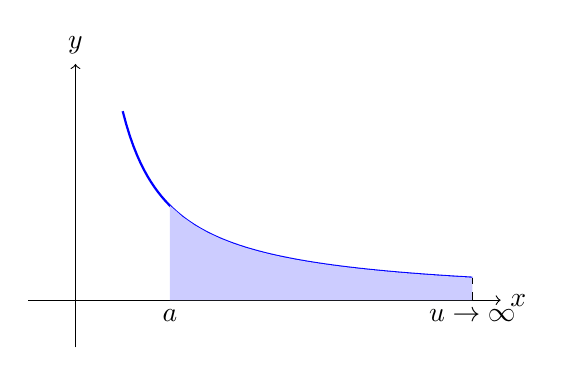
\begin{tikzpicture}[scale=1.2]
    \draw[->] (-0.5,0) -- (4.5,0) node[right] {$x$};
    \draw[->] (0,-0.5) -- (0,2.5) node[above] {$y$};
    \draw[thick, blue, samples=100, domain=0.5:4.2] plot (\x, {1/\x});
    \fill[blue!20, domain=1:4.2] (1,0) -- (1,1) -- plot (\x, {1/\x}) -- (4.2,0) -- cycle;
    \node at (2.5, 0.3) {};
    \draw[dashed] (4.2,0) -- (4.2, {1/4.2});
    \node[below] at (1,0) {$a$};
    \node[below] at (4.2,0) {$u \to \infty$};
\end{tikzpicture}
\caption{Visualizing an integral over an infinite interval}
\end{figure}

Similarly, we can define integrals for other infinite intervals:
\[
\int_{-\infty}^b f(x) dx = \lim_{u \to -\infty} \int_u^b f(x) dx
\]

\[
\int_{-\infty}^{+\infty} f(x) dx = \int_{-\infty}^c f(x) dx + \int_c^{+\infty} f(x) dx
\]

For the integral from $-\infty$ to $+\infty$ to converge, \textbf{both} constituent integrals must converge independently. The choice of the splitting point $c$ does not affect the convergence.
\subsubsection{Benchmark: The $p$-Integral (Type I)}
To determine the convergence of complex functions, we compare them to the power function $1/x^p$.

\begin{theorem}
The integral $\int_1^{+\infty} \frac{1}{x^p} \, dx$:
\begin{itemize}
    \item \textbf{Converges} if $p > 1$.
    \item \textbf{Diverges} if $p \leq 1$.
\end{itemize}
\end{theorem}
\begin{proof}
Evaluating $\int_1^u x^{-p} \, dx$:
\begin{itemize}
    \item If $p=1$, $\ln u \to \infty$ as $u \to \infty$.
    \item If $p \neq 1$, $\frac{u^{1-p}-1}{1-p}$. For convergence, we need $u^{1-p} \to 0$, which requires $1-p < 0 \implies p > 1$.
\end{itemize}
\end{proof}

\subsection{Improper Integrals of the Second Kind (Unbounded Functions)}

These integrals occur on a finite interval $[a,b]$ where the integrand $f(x)$ becomes infinite (has a singularity) at one or more points.

\begin{definition}
If $f$ is continuous on $[a, b)$ and discontinuous at $b$ (e.g., $\lim_{x \to b^-} |f(x)| = \infty$), we define:
\[
\int_a^b f(x) \, dx = \lim_{\epsilon \to 0^+} \int_a^{b-\epsilon} f(x) \, dx
\]
\end{definition}

\subsubsection{Benchmark: The $p$-Integral (Type II)}
Be careful: the convergence condition for singularities is the \textit{reverse} of infinite intervals.

\begin{theorem}
For the interval $(0, 1]$, the integral $\int_0^1 \frac{1}{x^p} \, dx$:
\begin{itemize}
    \item \textbf{Converges} if $p < 1$.
    \item \textbf{Diverges} if $p \geq 1$.
\end{itemize}
\end{theorem}

\subsection{General Theory of Convergence}

Before applying practical tests, we establish the rigorous necessary and sufficient conditions for convergence.

\subsubsection{Cauchy Criterion}
The Cauchy Criterion is fundamental because it allows us to prove convergence without knowing the limit's value.

\begin{theorem}[Cauchy Criterion for Improper Integrals]
The integral $\int_a^{+\infty} f(x) \, dx$ converges \textbf{if and only if} for every $\epsilon > 0$, there exists an $M > a$ such that for all $u_2 > u_1 > M$:
\[
\left| \int_{u_1}^{u_2} f(x) \, dx \right| < \epsilon
\]
\end{theorem}

\subsubsection{Absolute vs. Conditional Convergence}
\begin{itemize}
    \item \textbf{Absolute Convergence:} $\int |f(x)| \, dx$ converges.
    \item \textbf{Conditional Convergence:} $\int f(x) \, dx$ converges, but $\int |f(x)| \, dx$ diverges.
\end{itemize}
\begin{theorem}
If $\int_a^{+\infty} |f(x)| \, dx$ converges, then $\int_a^{+\infty} f(x) \, dx$ converges.
\end{theorem}

\subsection{Convergence Tests}

\subsubsection{Direct Comparison Test}
\begin{theorem}
Let $f(x)$ and $g(x)$ be continuous functions on $[a, +\infty)$ such that $0 \leq f(x) \leq g(x)$ for all $x \geq a$.
\begin{enumerate}
    \item If $\int_a^{+\infty} g(x) dx$ converges, then $\int_a^{+\infty} f(x) dx$ also converges.
    \item If $\int_a^{+\infty} f(x) dx$ diverges, then $\int_a^{+\infty} g(x) dx$ also diverges.
\end{enumerate}
\end{theorem}
\textit{Intuition:} If the area under the larger curve is finite, the area under the smaller curve must be finite. If the area under the smaller curve is infinite, the larger area must be infinite.
\begin{example}

Does $\int_1^{+\infty} \frac{\sin^2 x}{x^2} dx$ converge?
\end{example}
\textbf{Solution:} We know that $0 \leq \sin^2 x \leq 1$. Therefore:
\[
0 \leq \frac{\sin^2 x}{x^2} \leq \frac{1}{x^2}
\]
We know that $\int_1^{+\infty} \frac{1}{x^2} dx$ converges ($p=2 > 1$). By the Direct Comparison Test, $\int_1^{+\infty} \frac{\sin^2 x}{x^2} dx$ converges.
\subsubsection{Limit Comparison Test}

Sometimes finding a direct inequality is difficult. The Limit Comparison Test is often more powerful.

\begin{theorem}
Let $f(x)$ and $g(x)$ be positive continuous functions on $[a, +\infty)$. If:
\[
\lim_{x \to +\infty} \frac{f(x)}{g(x)} = L
\]
where $0 < L < +\infty$, then $\int_a^{+\infty} f(x) dx$ and $\int_a^{+\infty} g(x) dx$ either both converge or both diverge.
\end{theorem}
If $L=0$ and $g(x)$ converges, then $f(x)$ converges. If $L=+\infty$ and $g(x)$ diverges, then $f(x)$ diverges.
\begin{example}
Analyze $\int_1^{+\infty} \frac{x}{1+x^3} dx$.
\end{example}

\textbf{Solution:} For large $x$, the term $1$ is negligible, so $\frac{x}{1+x^3} \approx \frac{x}{x^3} = \frac{1}{x^2}$.

Let $f(x) = \frac{x}{1+x^3}$ and $g(x) = \frac{1}{x^2}$.

\[
\lim_{x \to +\infty} \frac{f(x)}{g(x)} = \lim_{x \to +\infty} \frac{x/(1+x^3)}{1/x^2} = \lim_{x \to +\infty} \frac{x^3}{1+x^3} = 1
\]

Since $L=1$ (finite and positive) and we know $\int_1^{+\infty} \frac{1}{x^2} dx$ converges, the original integral converges.



For positive functions, we use comparison tests. For oscillating functions, we need more advanced tools.

\subsubsection{Cauchy's Limit Comparison Test (Order Analysis)}
This is the most practical method for determining convergence. It formalizes the idea of comparing a function to $1/x^p$.

\begin{theorem}
Let $f(x)$ be a positive function defined on $[a, +\infty)$. Consider the limit of $f(x)$ multiplied by a test power $x^p$:
\[
\lambda = \lim_{x \to +\infty} x^p f(x)
\]
\begin{enumerate}
    \item \textbf{Convergence Case:} If we can find a $p > 1$ such that $0 \le \lambda < +\infty$, then $\int_a^{+\infty} f(x) \, dx$ \textbf{converges}.
    \textit{(Meaning: $f(x)$ goes to zero faster than $1/x$, roughly like $1/x^p$)}
    
    \item \textbf{Divergence Case:} If we can find a $p \le 1$ such that $0 < \lambda \le +\infty$, then $\int_a^{+\infty} f(x) \, dx$ \textbf{diverges}.
    \textit{(Meaning: $f(x)$ goes to zero slower than or equal to $1/x$)}
\end{enumerate}
\end{theorem}

\begin{example}
Test $\int_1^{+\infty} \frac{\ln x}{x^2} \, dx$.
We suspect convergence because $x^2$ dominates. Let's compare with $p=1.5$ (since $1 < 1.5 < 2$, giving us "room").
\[
\lim_{x \to +\infty} x^{1.5} \frac{\ln x}{x^2} = \lim_{x \to +\infty} \frac{\ln x}{x^{0.5}} = 0 \quad (\text{by L'Hopital})
\]
Since $p=1.5 > 1$ and the limit is finite, the integral converges.
\end{example}

\subsubsection{Dirichlet and Abel Tests (For Conditional Convergence)}
These tests are used for integrals of the product form $\int_a^{+\infty} f(x)g(x) \, dx$, typically where one part oscillates and the other decays.

\begin{theorem}[Dirichlet's Test]
The integral $\int_a^{+\infty} f(x)g(x) \, dx$ converges if:
\begin{enumerate}
    \item $f(x)$ has bounded partial integrals: $\exists M, \forall u > a, |\int_a^u f(t) \, dt| \le M$.
    \item $g(x)$ is monotonic decreasing and $\lim_{x \to +\infty} g(x) = 0$.
\end{enumerate}
\end{theorem}
\textit{Classic Application:} $\int_0^{+\infty} \frac{\sin x}{x} \, dx$. Here $f(x)=\sin x$ (bounded integral) and $g(x)=1/x$ (monotonic to 0).

\begin{theorem}[Abel's Test]
The integral $\int_a^{+\infty} f(x)g(x) \, dx$ converges if:
\begin{enumerate}
    \item $\int_a^{+\infty} f(x) \, dx$ converges (the integral itself).
    \item $g(x)$ is monotonic and bounded.
\end{enumerate}
\end{theorem}

\subsubsection{Cauchy Principal Value (P.V.)}

In some divergent integrals, the positive and negative areas might cancel each other out if limits are taken symmetrically. This value is called the Cauchy Principal Value.

\begin{definition}
\begin{enumerate}
    \item For singularities at $c \in (a, b)$:
    \[
    \text{P.V.} \int_a^b f(x) \, dx = \lim_{\epsilon \to 0^+} \left( \int_a^{c-\epsilon} f(x) \, dx + \int_{c+\epsilon}^b f(x) \, dx \right)
    \]
    \item For infinite intervals $(-\infty, +\infty)$:
    \[
    \text{P.V.} \int_{-\infty}^{+\infty} f(x) \, dx = \lim_{R \to +\infty} \int_{-R}^R f(x) \, dx
    \]
\end{enumerate}
\end{definition}

\begin{remark}
\textbf{Convergence $\implies$ P.V. exists}, but the converse is false.
\end{remark}

\begin{example}
Consider $f(x) = \frac{1}{x}$ on $[-1, 1]$.
\begin{itemize}
    \item \textbf{Improper Integral:} $\int_{-1}^1 \frac{1}{x} \, dx = \int_{-1}^0 \frac{1}{x} \, dx + \int_0^1 \frac{1}{x} \, dx$.
    Since $\int_{\epsilon}^1 \frac{1}{x} \, dx = -\ln \epsilon \to \infty$, the standard integral \textbf{diverges}.
    \item \textbf{Principal Value:}
    \[
    \text{P.V.} \int_{-1}^1 \frac{1}{x} \, dx = \lim_{\epsilon \to 0^+} \left( \int_{-1}^{-\epsilon} \frac{1}{x} \, dx + \int_{\epsilon}^1 \frac{1}{x} \, dx \right) = 0
    \]
    (Due to the odd symmetry of the function).
\end{itemize}
\end{example}

\subsubsection{Comprehensive Example: The Gamma Function}
\[
\Gamma(s) = \int_0^{+\infty} x^{s-1} e^{-x} \, dx
\]
This integral requires analysis of both singularity and infinite bounds.
\begin{itemize}
    \item \textbf{At $0$:} If $s < 1$, $x^{s-1}$ has a singularity. Since $e^{-x} \approx 1$, it behaves like $\int_0^1 \frac{1}{x^{1-s}} dx$. By the Type II $p$-test, this converges if $1-s < 1 \implies s > 0$.
    \item \textbf{At $+\infty$:} $e^{-x}$ decays faster than any power $x^p$ grows. Using the Limit Comparison Test with $1/x^2$:
    \[
    \lim_{x \to \infty} x^2 (x^{s-1} e^{-x}) = 0
    \]
    Thus, it converges for all $s$.
\end{itemize}
\textbf{Conclusion:} The integral converges for $s > 0$.

At the end of this chapter, let's use the knowledge we learned to solve an interesting problem: the Gabriel's Horn.

Considering we have a horn, whose cross section is a circle but longitudinal section is function $y = \frac{1}{x}, x \in (1,\infty)$.

Let's first calculate the volume of the horn:

\[V = \pi \int_{1}^{+\infty} (\frac{1}{x})^2 dx = \pi [-\frac{1}{x}]_{1}^{+\infty} = \pi\]

We can see that the horn have finite volume.

Then calculate the surface area of the horn.

\[
S = 2\pi \int_{1}^{+\infty} \frac{1}{x} \sqrt{1+\frac{1}{x^4}} dx \geq 2\pi \int_{1}^{+\infty} \frac{1}{x} dx = +\infty
\]

The integration product of the surface area is divergent.

Here comes a very interesting paradox. We can use finite many paint to fill the horn, but this horn of paint cannot coated the inner wall of the horn.

This consequence is contradicting to our naive understanding.

As we close this chapter, remember that this is not an end, but a gateway. The journey of mathematical analysis continues: in the \textbf{Chapter 4}, we will extend these foundations to higher dimensions, study curves and surfaces in greater depth, and encounter even more beautiful and unexpected results. The horn's call, echoing from the realm of the infinite, invites us to explore further.

In later chapters, we will move on to more advanced topics in analysis, such as multi-variables calculus, differential equations, complex analysis and functional analysis. Each of these areas builds upon the concepts we have developed here, and each offers its own unique insights and challenges. We encourage readers to continue their exploration, armed with the rigorous tools and deep understanding gained from this chapter.


\vspace{1cm}
\noindent
\textbf{References:} \\
Mathematical Analysis (Third Edition), Chen, J., Higher Education Press \\
The Real Numbers and Real Analysis, Ethan D. Bloch, Springer



\chapter{Linear Algebra}
\begin{quote}
\emph{
So long after we finished the first part of the analysis section, we will now move on to the new chapter: Linear Algebra. It's a completely new part of mathematics.
}

\emph{
Unlike analysis and calculus, linear algebra requires more geometric understanding. Here, proof is still important. But what is more crucial for learners is to construct geometric intuition for the subject. We would like to claim that intuition is different from imagination. Though we can only imagine the three dimensional Euclidean space, but our intuition can bring us forward to higher dimension, and more abstract linear spaces.
}

\emph{
In this part, we will start from the topic of solving Systems of Linear Equations, then we will move on to study a special kind of linear space: the Vector Space. Finally, we will move on to a more abstract part: the Linear Space, this equipped us with a new tool to study more general forms of algebraic structure and system.
}

\emph{
Specifically, in the final part focusing on abstract Linear Spaces, we will delve into key concepts such as linear independence, basis, dimension, and linear transformations. Understanding these foundational ideas allows us to unify seemingly disparate mathematical objects—like functions, polynomials, and matrices—under a single, powerful framework. This abstraction is not just an academic exercise; it provides the essential language and tools for tackling complex problems in fields ranging from differential equations and data science to quantum mechanics and engineering optimization. The geometric intuition developed in the study of $\mathbb{R}^n$ will prove indispensable as we navigate these higher-dimensional, abstract realms, cementing linear algebra as one of the most fundamental and broadly applicable areas of modern mathematics.
}

\emph{
In latter chapters, we will introduce another branch of Algebra, the abstract algebra. Unlike Linear algebra that focused more on multivariate equations, abstract algebra study the solution structure of higher-degree equations, which is an even more abstract part of mathematics. But even in abstract algebra we still need the knowledge about linear algebra. So now, let's get started.
}
\end{quote}

\section{Linear Equations and Matrices}

\subsection{Systems of Linear Equations}

I believe most of the readers have seen systems of equations like this:

\[
\begin{cases}
x+y=1\\
x-y =0
\end{cases}
\]

They might have different numbers of variables and equations, but they all shared the same feature: \textbf{Each equation is linear.} Variables are raised only to the first power, with no products between variables (like $xy$), or nonlinear functions (e.g., $\sin(x)$ or $\sqrt{x}$).

For such kind of equation system, we call it the \textbf{system of linear equations}. Their general expression has $m$ equations and $n$ variables (also called an $m \times n$ system):

\[
\begin{cases}
a_{11}x_1 + a_{12}x_2 + \cdots + a_{1n}x_n = b_1\\
a_{21}x_1 + a_{22}x_2 + \cdots + a_{2n}x_n = b_2\\
\quad \vdots \\
a_{m1}x_1 + a_{m2}x_2 + \cdots + a_{mn}x_n = b_m
\end{cases}
\]
Here, $x_1, \ldots, x_n$ are the \textbf{variables} (unknowns), the $a_{ij}$ are the \textbf{coefficients}, and $b_1, \ldots, b_m$ are the \textbf{constant terms}.

A \textbf{solution} to the system is a set of numbers $(s_1, s_2, \ldots, s_n)$ that satisfies all $m$ equations simultaneously when substituted for $(x_1, x_2, \ldots, x_n)$. The set of all possible solutions is called the \textbf{solution set}.

\begin{example}[A 2x2 System]
Consider the system:
\[
\begin{cases}
x_1 + x_2 = 3 \\
x_1 - x_2 = -1
\end{cases}
\]
We can solve this using simple algebra.
\begin{enumerate}
    \item \textbf{Substitution:} From the first equation, $x_2 = 3 - x_1$. Substitute this into the second: $x_1 - (3 - x_1) = -1$, which gives $2x_1 - 3 = -1$, so $2x_1 = 2$, and $x_1 = 1$. Then $x_2 = 3 - 1 = 2$. The unique solution is $(1, 2)$.
    \item \textbf{Elimination:} Add the two equations: $(x_1 + x_2) + (x_1 - x_2) = 3 + (-1)$, which gives $2x_1 = 2$, so $x_1 = 1$. Subtract the second from the first: $(x_1 + x_2) - (x_1 - x_2) = 3 - (-1)$, which gives $2x_2 = 4$, so $x_2 = 2$.
\end{enumerate}
The solution set is the single point $(1, 2)$.
\end{example}

In linear algebra, we are interested in three questions:
\begin{enumerate}
    \item \textbf{Existence:} Does a solution exist? (Is the system \textbf{consistent}?)
    \item \textbf{Uniqueness:} If a solution exists, is it the only one?
    \item \textbf{Computation:} If solutions exist, how do we find them?
\end{enumerate}

Geometrically, for a 2x2 system, each equation represents a line in the $\mathbb{R}^2$ plane. The solution set is the intersection of these lines.
\begin{itemize}
    \item \textbf{Unique Solution:} The lines intersect at a single point.
    \item \textbf{No Solution:} The lines are parallel and distinct.
    \item \textbf{Infinitely Many Solutions:} The two equations represent the same line.
\end{itemize}
% 

For a 3x3 system, each equation is a plane in $\mathbb{R}^3$. The solution set is the intersection of these three planes, which could be a point, a line, a plane, or empty.
% 

The methods of substitution and elimination become extremely cumbersome for larger systems (e.g., 5 equations, 5 variables). We need a more systematic and efficient approach. This is where matrices come in.

\subsection{Matrix Algebra}

\subsubsection{Matrix Notation and Special Matrices}

The essence of our new method is to manipulate the equations without changing their solution set. We observe that all the information of the system is contained in the coefficients $a_{ij}$ and the constant terms $b_i$. The variable names $x_1, x_2, \ldots$ are just placeholders. We can therefore encode the entire system into a compact rectangular array called a \textbf{matrix}.

\begin{definition}
A \textbf{matrix} is a rectangular array of numbers, called \textbf{entries} or \textbf{elements}. A matrix with $m$ rows and $n$ columns is called an $m \times n$ matrix (read "m by n").
\end{definition}

For the general linear system, we define two key matrices.

The \textbf{coefficient matrix} is:
\[ \textbf{A} = \begin{pmatrix}
a_{11} & a_{12} & \cdots & a_{1n} \\
a_{21} & a_{22} & \cdots & a_{2n} \\
\vdots & \vdots & \ddots & \vdots \\
a_{m1} & a_{m2} & \cdots & a_{mn}
\end{pmatrix} \]
We can denote this matrix as $A = [a_{ij}]$. $a_{ij}$ represents the element in the $i$-th row and $j$-th column.

The \textbf{augmented matrix}, which includes the constant terms, is:
\[ (A \mid \mathbf{b}) = \left(\begin{array}{cccc|c}
a_{11} & a_{12} & \cdots & a_{1n} & b_1 \\
a_{21} & a_{22} & \cdots & a_{2n} & b_2 \\
\vdots & \vdots & \ddots & \vdots & \vdots \\
a_{m1} & a_{m2} & \cdots & a_{mn} & b_m
\end{array}\right) \]
Solving the system is now equivalent to manipulating this augmented matrix.

\begin{example}
The system
\[
\begin{cases}
x_1 - 2x_2 + x_3 = 0 \\
2x_2 - 8x_3 = 8 \\
5x_1 - 5x_3 = 10
\end{cases}
\]
has the coefficient matrix
\[ A = \begin{pmatrix} 1 & -2 & 1 \\ 0 & 2 & -8 \\ 5 & 0 & -5 \end{pmatrix} \]
and the augmented matrix
\[ (A \mid \mathbf{b}) = \left(\begin{array}{ccc|c} 1 & -2 & 1 & 0 \\ 0 & 2 & -8 & 8 \\ 5 & 0 & -5 & 10 \end{array}\right) \]
\end{example}

\paragraph{Matrix Terminology and Special Matrices}

\begin{itemize}
    \item \textbf{Size/Dimension:} A matrix $A$ with $m$ rows and $n$ columns has size $m \times n$.
    \item \textbf{Square Matrix:} A matrix is \textbf{square} if its number of rows equals its number of columns ($m=n$).
    \item \textbf{Equality:} Two matrices $A = [a_{ij}]$ and $B = [b_{ij}]$ are \textbf{equal} if and only if they have the same size ($m \times n$) and all their corresponding entries are equal ($a_{ij} = b_{ij}$ for all $i, j$).
    \item \textbf{Principal Diagonal:} In a square matrix, the entries $a_{11}, a_{22}, \ldots, a_{nn}$ form the \textbf{principal diagonal} (or main diagonal).
    \item \textbf{Auxiliary Diagonal:} In a square matrix, the diagonal from the upper right to the lower left ($a_{1n}, a_{2,n-1}, \ldots, a_{n1}$) is the \textbf{auxiliary diagonal}.
\end{itemize}

There are several special types of matrices:

% 

\begin{enumerate}
    \item \textbf{Null matrix (Zero matrix):} A matrix (of any size) where all entries are 0. It is often denoted $\mathbf{0}$ or $\mathbf{0}_{m \times n}$.
    \[ \mathbf{0} = \begin{pmatrix} 0 & 0 & \cdots & 0 \\ \vdots & \vdots & \ddots & \vdots \\ 0 & 0 & \cdots & 0 \end{pmatrix} \]
    \item \textbf{Identity matrix:} A square matrix $I_n$ (or just $I$) whose entries on the principal diagonal are all 1, and all other entries are 0.
    \[ I_3 = \begin{pmatrix} 1 & 0 & 0 \\ 0 & 1 & 0 \\ 0 & 0 & 1 \end{pmatrix} \]
    The identity matrix is the multiplicative identity: $AI = A$ and $IA = A$ (for compatible sizes).
    \item \textbf{Diagonal matrix:} A square matrix where all entries \emph{off} the principal diagonal are 0.
    \[ D = \begin{pmatrix} 3 & 0 & 0 \\ 0 & -1 & 0 \\ 0 & 0 & 5 \end{pmatrix} \]
    \item \textbf{Upper triangular matrix:} A square matrix whose entries \emph{below} the principal diagonal are all 0 ($a_{ij} = 0$ for $i > j$).
    \[ U = \begin{pmatrix} 1 & 4 & -1 \\ 0 & 2 & 7 \\ 0 & 0 & 3 \end{pmatrix} \]
    \item \textbf{Lower triangular matrix:} A square matrix whose entries \emph{above} the principal diagonal are all 0 ($a_{ij} = 0$ for $i < j$).
    \[ L = \begin{pmatrix} 1 & 0 & 0 \\ 5 & 2 & 0 \\ -1 & 0 & 3 \end{pmatrix} \]
    \item \textbf{Transpose:} The \textbf{transpose} of an $m \times n$ matrix $A$, denoted $A^T$ (or $A'$), is the $n \times m$ matrix obtained by interchanging its rows and columns. That is, $(A^T)_{ij} = A_{ji}$.
    \[ A = \begin{pmatrix} 1 & 2 & 3 \\ 4 & 5 & 6 \end{pmatrix} \quad \implies \quad A^T = \begin{pmatrix} 1 & 4 \\ 2 & 5 \\ 3 & 6 \end{pmatrix} \]
    \item \textbf{Symmetric matrix:} A square matrix $A$ such that $A^T = A$. This means $a_{ij} = a_{ji}$ for all $i, j$.
    \[ S = \begin{pmatrix} 1 & 5 & -1 \\ 5 & 2 & 0 \\ -1 & 0 & 3 \end{pmatrix} \]
    \item \textbf{Skew-symmetric matrix:} A square matrix $A$ such that $A^T = -A$. This means $a_{ij} = -a_{ji}$ (and $a_{ii} = 0$).
    \[ K = \begin{pmatrix} 0 & 5 & -1 \\ -5 & 0 & 2 \\ 1 & -2 & 0 \end{pmatrix} \]
\end{enumerate}

\subsubsection{Matrix Operations}

We can define algebraic operations on matrices.

\paragraph{Matrix Addition and Scalar Multiplication}
\begin{definition}
Let $A = [a_{ij}]$ and $B = [b_{ij}]$ be two matrices of the \textbf{same size} $m \times n$.
\begin{enumerate}
    \item \textbf{Addition:} Their sum $A+B$ is the $m \times n$ matrix $C = [c_{ij}]$ where $c_{ij} = a_{ij} + b_{ij}$.
    \item \textbf{Scalar Multiplication:} Let $c$ be a scalar (a real number). The scalar multiple $cA$ is the $m \times n$ matrix $D = [d_{ij}]$ where $d_{ij} = c \cdot a_{ij}$.
\end{enumerate}
Matrix subtraction is defined as $A - B = A + (-1)B$.
\end{definition}

\begin{example}
Let $A = \begin{pmatrix} 1 & 2 \\ 3 & 4 \end{pmatrix}$ and $B = \begin{pmatrix} 5 & 0 \\ -1 & 7 \end{pmatrix}$.
Then
\[ A+B = \begin{pmatrix} 1+5 & 2+0 \\ 3-1 & 4+7 \end{pmatrix} = \begin{pmatrix} 6 & 2 \\ 2 & 11 \end{pmatrix} \]
\[ 3A = \begin{pmatrix} 3(1) & 3(2) \\ 3(3) & 3(4) \end{pmatrix} = \begin{pmatrix} 3 & 6 \\ 9 & 12 \end{pmatrix} \]
Note that $A + \begin{pmatrix} 1 & 2 & 3 \\ 4 & 5 & 6 \end{pmatrix}$ is \textbf{undefined} as the sizes do not match.
\end{example}

These operations obey familiar properties:
\begin{property}[Properties of Addition and Scalar Multiplication]
Let $A, B, C$ be $m \times n$ matrices and $c, d$ be scalars.
\begin{enumerate}
    \item $A+B = B+A$ (Commutativity of Addition)
    \item $(A+B)+C = A+(B+C)$ (Associativity of Addition)
    \item $A + \mathbf{0} = A$ (Additive Identity)
    \item $A + (-A) = \mathbf{0}$ (Additive Inverse)
    \item $c(A+B) = cA + cB$ (Distributivity)
    \item $(c+d)A = cA + dA$ (Distributivity)
    \item $c(dA) = (cd)A$
    \item $1A = A$
\end{enumerate}
\end{property}
\begin{remark}
These 8 properties, plus closure, are precisely the axioms of a \textbf{Vector Space}. The set $M_{m \times n}$ of all $m \times n$ matrices is a prime example of a vector space.
\end{remark}

\newpage

\paragraph{Matrix Multiplication}
This operation is more complex and profoundly important.

\begin{definition}[Matrix Multiplication]
Let $A$ be an $m \times \mathbf{n}$ matrix and $B$ be an $\mathbf{n} \times p$ matrix. Their \textbf{product} $AB$ is an $m \times p$ matrix $C = [c_{ij}]$.
The entry $c_{ij}$ in the $i$-th row and $j$-th column of $AB$ is computed by taking the \textbf{dot product} of the $i$-th row of $A$ and the $j$-th column of $B$.
\[ c_{ij} = (\text{Row } i \text{ of } A) \cdot (\text{Column } j \text{ of } B) = a_{i1}b_{1j} + a_{i2}b_{2j} + \cdots + a_{in}b_{nj} \]
\[ c_{ij} = \sum_{k=1}^{n} a_{ik}b_{kj} \]
\end{definition}

\textbf{Crucial Note:} The product $AB$ is only defined if the \textbf{number of columns in A} equals the \textbf{number of rows in B}.
\[
(m \times \mathbf{n}) \cdot (\mathbf{n} \times p) \to (m \times p)
\]

\begin{example}
Let $A = \begin{pmatrix} 1 & 2 & 3 \\ 4 & 5 & 6 \end{pmatrix}$ ($2 \times 3$) and $B = \begin{pmatrix} 7 & 8 \\ 9 & 0 \\ 1 & 2 \end{pmatrix}$ ($3 \times 2$).
The product $AB$ will be a $2 \times 2$ matrix.
\[
AB = \begin{pmatrix}
(1\cdot 7 + 2\cdot 9 + 3\cdot 1) & (1\cdot 8 + 2\cdot 0 + 3\cdot 2) \\
(4\cdot 7 + 5\cdot 9 + 6\cdot 1) & (4\cdot 8 + 5\cdot 0 + 6\cdot 2)
\end{pmatrix}
= \begin{pmatrix}
(7 + 18 + 3) & (8 + 0 + 6) \\
(28 + 45 + 6) & (32 + 0 + 12)
\end{pmatrix}
= \begin{pmatrix} 28 & 14 \\ 79 & 44 \end{pmatrix}
\]
Now let's compute $BA$. This will be a $3 \times 3$ matrix.
\[
BA = \begin{pmatrix} 7 & 8 \\ 9 & 0 \\ 1 & 2 \end{pmatrix} \begin{pmatrix} 1 & 2 & 3 \\ 4 & 5 & 6 \end{pmatrix}
= \begin{pmatrix}
(7\cdot 1 + 8\cdot 4) & (7\cdot 2 + 8\cdot 5) & (7\cdot 3 + 8\cdot 6) \\
(9\cdot 1 + 0\cdot 4) & (9\cdot 2 + 0\cdot 5) & (9\cdot 3 + 0\cdot 6) \\
(1\cdot 1 + 2\cdot 4) & (1\cdot 2 + 2\cdot 5) & (1\cdot 3 + 2\cdot 6)
\end{pmatrix}
= \begin{pmatrix} 39 & 54 & 69 \\ 9 & 18 & 27 \\ 9 & 12 & 15 \end{pmatrix}
\]
\end{example}

\begin{property}[Properties of Matrix Multiplication]
Let $A, B, C$ be matrices of compatible sizes and $c$ be a scalar.
\begin{enumerate}
    \item \textbf{Warning:} $AB \neq BA$ in general. Matrix multiplication is \textbf{not commutative}. (See example above).
    \item $A(BC) = (AB)C$ (Associativity)
    \item $A(B+C) = AB + AC$ (Left Distributivity)
    \item $(A+B)C = AC + BC$ (Right Distributivity)
    \item $c(AB) = (cA)B = A(cB)$
    \item $I_m A = A = A I_n$ (Multiplicative Identity)
\end{enumerate}
\end{property}

But we still want the multiplication to have such kind of property like $AB = BA$, we will introduce a special kind of matrix in later chapters that can satisfy this property.

The prooves of the properties above are left for readers.

\begin{remark}
Remember, $\textbf{A} \textbf{b} = \textbf{0}$ can not deduce $A=0$ or $B=0$. This is another counterexample against our common sense of algebraic calculations.
\end{remark}

\begin{definition}
Assume we have a square matrix with $n$ orders, and a number $m \in \mathbb{N}^{*}$, then we call the product of m copies of $A$ "$A$ to the m-th power", denoted as $A^m$
Specifically, we define $A^0 = I_n$.
\end{definition}

The calculations of power is \textbf{BASICALLY} the same with the regular rules. Except those have requirement with the orders of multiplication. Like:

\[(A+B)^2 = A^2 + AB + BA + B^2\]
\[(A+B)(A-B) = A^2 - AB + BA - B^2\]

\begin{definition}
Assume $A=(a_{ij})_{m \times n}$, we define $A^T=(b_{kl})_{n \times m}$ the transpose of matrix $A$, iff $b_{kl} = a_{lk}, (k=1,2,\cdots,n,l=1,2,\cdots,m)$
\end{definition}

\begin{property}[Properties of the Transpose]
\begin{enumerate}
    \item $(A^T)^T = A$
    \item $(A+B)^T = A^T + B^T$
    \item $(cA)^T = cA^T$
    \item \textbf{(Reversal Property)} $(AB)^T = B^T A^T$
    \item $(A^m)^T = (A^T)^m$
\end{enumerate}
\end{property}
\begin{proof}[Proof of $(AB)^T = B^T A^T$]
Let $A$ be $m \times n$ and $B$ be $n \times p$. $AB$ is $m \times p$, so $(AB)^T$ is $p \times m$.
$B^T$ is $p \times n$ and $A^T$ is $n \times m$, so $B^T A^T$ is also $p \times m$. They have the same size.
Let $C = AB$. The $(i, j)$-entry of $C^T$ is $C_{ji}$.
By definition, $C_{ji} = \sum_{k=1}^n A_{jk} B_{ki}$.
Now let $D = B^T A^T$. The $(i, j)$-entry of $D$ is:
\[ D_{ij} = \sum_{k=1}^n (B^T)_{ik} (A^T)_{kj} \]
By definition of transpose, $(B^T)_{ik} = B_{ki}$ and $(A^T)_{kj} = A_{jk}$.
So, $D_{ij} = \sum_{k=1}^n B_{ki} A_{jk} = \sum_{k=1}^n A_{jk} B_{ki}$.
Thus, $D_{ij} = C_{ji} = (C^T)_{ij}$. Since all entries are equal, $B^T A^T = (AB)^T$.
\end{proof}

There is also another important value for square matrix, we will use it in later contents.

\begin{definition}[The trace of matrix]
Assume a square matrix $A$ with $n$ orders $A=(a_{ij})$, $\sum_{i=1}^{n} a_{ii}$ is called the trace of matrix, denoted as $tr(A)$
\end{definition}

\begin{property}
\begin{enumerate}
    \item $tr(A+B) = tr(A) + tr(B)$
    \item $tr(kA) = k tr(A)$
    \item $tr(AB) = tr(BA)$
    \item $tr(A^T) = tr(A)$
\end{enumerate}
\end{property}

\subsubsection*{Definition of Block Matrices}
A block matrix is a matrix that is partitioned into smaller submatrices called \textbf{blocks}. This is done by drawing horizontal and vertical lines that divide the matrix into rectangular blocks. Partitioning allows us to view a large matrix as composed of smaller, more manageable parts.

If \( A \) is an \( m \times n \) matrix, we can partition it as follows:
\[
A = \begin{bmatrix}
    A_{11} & A_{12} & \cdots & A_{1q} \\
    A_{21} & A_{22} & \cdots & A_{2q} \\
    \vdots & \vdots & \ddots & \vdots \\
    A_{p1} & A_{p2} & \cdots & A_{pq}
\end{bmatrix}
\]
Here, each \( A_{ij} \) is a submatrix (block) of \( A \), and the dimensions of the blocks must be consistent: the number of columns in \( A_{ik} \) must equal the number of columns in \( A_{jk} \) for all \( i, j, k \), and similarly for rows.

\textbf{Operations with Block Matrices}

\paragraph*{Block Matrix Addition}
If two matrices \( A \) and \( B \) are partitioned into blocks with the \textbf{same dimensions} for corresponding blocks, they can be added block-wise:
\[
A + B = \begin{bmatrix}
    A_{11} + B_{11} & A_{12} + B_{12} & \cdots \\
    A_{21} + B_{21} & A_{22} + B_{22} & \cdots \\
    \vdots & \vdots & \ddots
\end{bmatrix}
\]
Each block \( A_{ij} \) and \( B_{ij} \) must have the same dimensions for the addition to be valid.

\paragraph*{Block Matrix Scalar Multiplication}
Scalar multiplication is performed by multiplying each block by the scalar:
\[
cA = \begin{bmatrix}
    cA_{11} & cA_{12} & \cdots \\
    cA_{21} & cA_{22} & \cdots \\
    \vdots & \vdots & \ddots
\end{bmatrix}
\]

\paragraph*{Block Matrix Multiplication}
If \( A \) is an \( m \times n \) block matrix and \( B \) is an \( n \times p \) block matrix, and the partitions are such that the number of column blocks of \( A \) equals the number of row blocks of \( B \), then the product \( C = AB \) can be computed block-wise:
\[
C_{ij} = \sum_{k=1}^{q} A_{ik} B_{kj}
\]
This requires that the number of columns in \( A_{ik} \) equals the number of rows in \( B_{kj} \) for each \( k \). The resulting block \( C_{ij} \) is the sum of products of corresponding blocks.

\textbf{Example:} If \( A = \begin{bmatrix} A_{11} & A_{12} \\ A_{21} & A_{22} \end{bmatrix} \) and \( B = \begin{bmatrix} B_{11} \\ B_{21} \end{bmatrix} \), then:
\[
AB = \begin{bmatrix}
    A_{11}B_{11} + A_{12}B_{21} \\
    A_{21}B_{11} + A_{22}B_{21}
\end{bmatrix}
\]

\paragraph*{Block Matrix Transpose}
The transpose of a block matrix is obtained by transposing each block and then transposing the block structure:
\[
A^\top = \begin{bmatrix}
    A_{11}^\top & A_{21}^\top & \cdots \\
    A_{12}^\top & A_{22}^\top & \cdots \\
    \vdots & \vdots & \ddots
\end{bmatrix}
\]
Note that the positions of the blocks are also transposed (e.g., the block in the (1,2) position becomes the block in the (2,1) position after transposition).

\paragraph*{Block Diagonal Matrices}
A block diagonal matrix is a square block matrix where all off-diagonal blocks are zero matrices:
\[
A = \begin{bmatrix}
    A_{11} & 0 & \cdots & 0 \\
    0 & A_{22} & \cdots & 0 \\
    \vdots & \vdots & \ddots & \vdots \\
    0 & 0 & \cdots & A_{pp}
\end{bmatrix}
\]
Operations on block diagonal matrices simplify because the blocks can be handled independently (e.g., the inverse of a block diagonal matrix is the block diagonal matrix of the inverses, if they exist).

\subsubsection*{Advantages of Using Block Matrices}
\begin{itemize}
    \item Simplifies operations on large matrices by breaking them into smaller parts.
    \item Facilitates parallel computation.
    \item Helps in proving theoretical results by induction on block structures.
    \item Commonly used in numerical linear algebra for efficient algorithms.
\end{itemize}


\begin{definition}
An $n \times n$ square matrix $A$ is \textbf{invertible} (or \textbf{non-singular}) if there exists an $n \times n$ matrix $B$ such that
\[ AB = I_n \quad \text{and} \quad BA = I_n \]
This matrix $B$ is unique and is called the \textbf{inverse} of $A$, denoted $A^{-1}$.
If no such matrix $B$ exists, $A$ is \textbf{singular} (or \textbf{non-invertible}).
\end{definition}



\begin{example}[Inverse of a 2x2 Matrix]
Let $A = \begin{pmatrix} a & b \\ c & d \end{pmatrix}$.
If $ad-bc \neq 0$, then $A$ is invertible and
\[ A^{-1} = \frac{1}{ad-bc} \begin{pmatrix} d & -b \\ -c & a \end{pmatrix} \]
If $ad-bc = 0$, $A$ is singular. The quantity $ad-bc$ is the \textbf{determinant} of $A$.
\end{example}

\begin{property}[Properties of Inverses]
Let $A$ and $B$ be invertible $n \times n$ matrices.
\begin{enumerate}
    \item $(A^{-1})^{-1} = A$
    \item $(AB)^{-1} = B^{-1} A^{-1}$ (Note the reversal of order)
    \item $(A^T)^{-1} = (A^{-1})^T$
    \item $(cA)^{-1} = \frac{1}{c} A^{-1}$ (for $c \neq 0$)
\end{enumerate}
\end{property}
\begin{proof}[Proof of $(AB)^{-1} = B^{-1} A^{-1}$]
We just need to check the definition.
\[ (AB)(B^{-1} A^{-1}) = A (B B^{-1}) A^{-1} = A (I) A^{-1} = A A^{-1} = I \]
\[ (B^{-1} A^{-1})(AB) = B^{-1} (A^{-1} A) B = B^{-1} (I) B = B^{-1} B = I \]
Since $B^{-1} A^{-1}$ satisfies the definition, it must be the inverse of $AB$.
\end{proof}

\subsection{Solving Systems of Linear Equations}

Now we return to our main problem: solving $m$ equations in $n$ variables.
The general idea, \textbf{Gaussian Elimination}, is to transform the augmented matrix into a simpler form from which we can just read off the solution.

\subsubsection{Elementary Row Operations (EROs)}

We can manipulate the augmented matrix using operations that correspond to manipulating the original equations. These operations \textbf{do not change the solution set}.

\begin{definition}
The three \textbf{elementary row operations (EROs)} are:
\begin{enumerate}
    \item \textbf{(Replacement)} Add to one row a multiple of another row. ($R_i \to R_i + cR_j$)
    \item \textbf{(Interchange)} Interchange two rows. ($R_i \leftrightarrow R_j$)
    \item \textbf{(Scaling)} Multiply all entries in a row by a non-zero constant. ($R_i \to cR_i, c \neq 0$)
\end{enumerate}
\end{definition}

\begin{definition}
Two matrices $A$ and $B$ are \textbf{row equivalent}, denoted $A \sim B$, if $B$ can be obtained from $A$ by a sequence of EROs.
\end{definition}

\begin{theorem}
If the augmented matrices of two linear systems are row equivalent, then the two systems have the \textbf{same solution set}.
\end{theorem}
\begin{proof}[Justification]
\begin{itemize}
    \item (Replacement) $R_i \to R_i + cR_j$ corresponds to adding $c$ times equation $j$ to equation $i$. This is a reversible step (by $R_i \to R_i - cR_j$), and any solution to the original system will also be a solution to the new one, and vice-versa.
    \item (Interchange) $R_i \leftrightarrow R_j$ corresponds to swapping the order of two equations, which clearly does not affect the solution set.
    \item (Scaling) $R_i \to cR_i$ (with $c \neq 0$) corresponds to multiplying an equation by $c$. This is reversible (by $R_i \to \frac{1}{c}R_i$), so it does not change the solution set.
\end{itemize}
\end{proof}

\subsubsection{Row Echelon Form and Rank}

The goal is to use EROs to simplify the matrix into a "staircase" form.

\begin{definition}
A matrix is in \textbf{Row Echelon Form (REF)} if it satisfies:
\begin{enumerate}
    \item All nonzero rows are above any rows of all zeros.
    \item Each \textbf{leading entry} (or \textbf{pivot}), which is the leftmost nonzero entry of a row, is in a column to the right of the leading entry of the row above it.
    \item All entries in a column \emph{below} a leading entry are zeros.
\end{enumerate}
\end{definition}

\begin{definition}
A matrix is in \textbf{Reduced Row Echelon Form (RREF)} if it is in REF and also satisfies:
\begin{enumerate}
    \item The leading entry in each nonzero row is 1.
    \item Each leading 1 is the \emph{only} nonzero entry in its column.
\end{enumerate}
\end{definition}



\begin{example}
\textbf{REF}:
\[ \begin{pmatrix} \fbox{2} & 3 & 4 & 5 \\ 0 & \fbox{1} & 6 & 7 \\ 0 & 0 & 0 & \fbox{8} \\ 0 & 0 & 0 & 0 \end{pmatrix} \]
\textbf{RREF}:
\[ \begin{pmatrix} \fbox{1} & 0 & -1 & 0 \\ 0 & \fbox{1} & 2 & 0 \\ 0 & 0 & 0 & \fbox{1} \\ 0 & 0 & 0 & 0 \end{pmatrix} \]
(Pivots are boxed.)
\end{example}

\begin{theorem}
Every matrix is row equivalent to a \textbf{unique} Reduced Row Echelon Form (RREF).
\end{theorem}

This algorithm to get to REF/RREF is the core of our solution method.

\begin{definition}
\begin{itemize}
    \item \textbf{Gaussian Elimination} is the process of using EROs to transform a matrix into REF.
    \item \textbf{Gauss-Jordan Elimination} is the process of using EROs to transform a matrix into RREF.
\end{itemize}
\end{definition}

\paragraph{The Algorithm (Gauss-Jordan Elimination)}
Let's solve a system completely.
\[
\begin{cases}
x_2 + 3x_3 = 4 \\
x_1 + x_2 + x_3 = 1 \\
2x_1 + 3x_2 + 4x_3 = 7
\end{cases}
\]
The augmented matrix is:
\[
\left(\begin{array}{ccc|c}
0 & 1 & 3 & 4 \\
1 & 1 & 1 & 1 \\
2 & 3 & 4 & 7
\end{array}\right)
\]
\textbf{Step 1: (Forward Phase - Get to REF)}
We need a pivot in the top-left (1,1) position. Swap with R2.
\[
\left(\begin{array}{ccc|c}
1 & 1 & 1 & 1 \\
0 & 1 & 3 & 4 \\
2 & 3 & 4 & 7
\end{array}\right) \quad (R_1 \leftrightarrow R_2)
\]
Create zeros below the first pivot.
\[
\left(\begin{array}{ccc|c}
1 & 1 & 1 & 1 \\
0 & 1 & 3 & 4 \\
0 & 1 & 2 & 5
\end{array}\right) \quad (R_3 \to R_3 - 2R_1)
\]
Now, move to the second pivot (2,2). It's already 1. Create a zero below it.
\[
\left(\begin{array}{ccc|c}
1 & 1 & 1 & 1 \\
0 & 1 & 3 & 4 \\
0 & 0 & -1 & 1
\end{array}\right) \quad (R_3 \to R_3 - R_2)
\]
The matrix is now in \textbf{Row Echelon Form}. This completes Gaussian Elimination.
We could stop here and use \textbf{back substitution}:
From $R_3$: $-x_3 = 1 \implies x_3 = -1$.
From $R_2$: $x_2 + 3x_3 = 4 \implies x_2 + 3(-1) = 4 \implies x_2 = 7$.
From $R_1$: $x_1 + x_2 + x_3 = 1 \implies x_1 + 7 + (-1) = 1 \implies x_1 = -5$.
The unique solution is $(-5, 7, -1)$.

\textbf{Step 2: (Backward Phase - Get to RREF)}
Continue from the REF. Scale all pivots to 1.
\[
\left(\begin{array}{ccc|c}
1 & 1 & 1 & 1 \\
0 & 1 & 3 & 4 \\
0 & 0 & 1 & -1
\end{array}\right) \quad (R_3 \to -1 \cdot R_3)
\]
Create zeros \emph{above} the pivots, starting from the rightmost pivot.
\[
\left(\begin{array}{ccc|c}
1 & 1 & 0 & 2 \\
0 & 1 & 0 & 7 \\
0 & 0 & 1 & -1
\end{array}\right) \quad (R_1 \to R_1 - R_3, R_2 \to R_2 - 3R_3)
\]
Create zero above the second pivot.
\[
\left(\begin{array}{ccc|c}
1 & 0 & 0 & -5 \\
0 & 1 & 0 & 7 \\
0 & 0 & 1 & -1
\end{array}\right) \quad (R_1 \to R_1 - R_2)
\]
This is the \textbf{Reduced Row Echelon Form}. The corresponding system is:
\[
\begin{cases}
x_1 = -5 \\
x_2 = 7 \\
x_3 = -1
\end{cases}
\]
This immediately gives the solution.

\newpage

\paragraph{Rank of a Matrix}
A key concept emerges from the echelon form.

\begin{definition}
The \textbf{rank} of a matrix $A$, denoted $\operatorname{rank}(A)$, is the number of leading entries (pivots) in its row echelon form. This number is unique for any given matrix.
\end{definition}

\begin{property}[Properties of Rank]
Let $A$ be an $m \times n$ matrix.
\begin{enumerate}
    \item $\operatorname{rank}(A) \le \min(m, n)$.
    \item $\operatorname{rank}(A) = 0$ if and only if $A = \mathbf{0}$.
    \item \textbf{(Major Theorem)} $\operatorname{rank}(A) = \operatorname{rank}(A^T)$. (The number of pivot rows equals the number of pivot columns).
    \item $\operatorname{rank}(AB) \le \min(\operatorname{rank}(A), \operatorname{rank}(B))$.
    \item $\operatorname{rank}(A+B) \le \operatorname{rank}(A) + \operatorname{rank}(B)$.
    \item $\operatorname{rank}(A)+\operatorname{rank}(B)-n \le \operatorname{rank}(AB)$
    \item If $P, Q$ are invertible, $\operatorname{rank}(PAQ) = \operatorname{rank}(A)$. EROs are equivalent to multiplying by an invertible matrix on the left, so row operations do not change the rank.
\end{enumerate}
In short, we can denote them as:
\[
\min \{r(A),r(B)\} \geq r(AB) \geq r(A) + r(B) - n
\]
\[
r(A+B) \leq r(A,B) \leq r \begin{pmatrix}
    A & O \\
    O & B
\end{pmatrix}
\]
\end{property}

\subsubsection{Solution Sets of Linear Systems}

The RREF of the \emph{augmented} matrix tells us everything about the solution set.
A \textbf{pivot column} is a column in the coefficient matrix $A$ that contains a pivot in its RREF.
Variables corresponding to pivot columns are called \textbf{basic variables}.
Variables corresponding to non-pivot columns are called \textbf{free variables}.

Let $r = \operatorname{rank}(A)$ for an $m \times n$ coefficient matrix $A$.
We analyze the RREF of the augmented matrix $[A \mid \mathbf{b}]$.

\begin{enumerate}
    \item \textbf{No Solution (Inconsistent System)}
    This occurs if the RREF of $[A \mid \mathbf{b}]$ has a row of the form $\begin{pmatrix} 0 & 0 & \cdots & 0 & \mid & 1 \end{pmatrix}$.
    This corresponds to the impossible equation $0x_1 + \cdots + 0x_n = 1$, or $0 = 1$.
    In terms of rank, this means the last column (the augmented column) is a pivot column.
    \textbf{Condition: $\operatorname{rank}(A) < \operatorname{rank}([A \mid \mathbf{b}])$.}

    \item \textbf{A Solution Exists (Consistent System)}
    This occurs if the augmented column is \emph{not} a pivot column.
    \textbf{Condition: $\operatorname{rank}(A) = \operatorname{rank}([A \mid \mathbf{b}])$.} Let this rank be $r$.
    \begin{itemize}
        \item \textbf{Unique Solution:} The system has a unique solution if there are \emph{no free variables}. This means every variable is a basic variable, so every column of $A$ is a pivot column.
        \textbf{Condition: $r = n$ (the number of variables).}
        
        \item \textbf{Infinitely Many Solutions:} The system has infinitely many solutions if there is \emph{at least one free variable}. This means some columns of $A$ are not pivot columns.
        \textbf{Condition: $r < n$ (the number of variables).}
        The $n - r$ free variables can be set to any arbitrary value (parameters), and the basic variables can be expressed in terms of them.
    \end{itemize}
\end{enumerate}

\paragraph{Parametric Vector Form}
When we have infinitely many solutions, we write the solution set in \textbf{parametric vector form}.

\begin{example}[Infinitely Many Solutions]
Find the general solution to the system with augmented matrix:
\[
\left(\begin{array}{ccc|c}
1 & 0 & -5 & 1 \\
0 & 1 & 1 & 4 \\
0 & 0 & 0 & 0
\end{array}\right)
\]
This matrix is already in RREF. The corresponding system is:
\[
\begin{cases}
x_1 - 5x_3 = 1 \\
x_2 + x_3 = 4 \\
0 = 0
\end{cases}
\]
The pivot columns are 1 and 2. So, $x_1$ and $x_2$ are \textbf{basic variables}.
Column 3 is not a pivot column. So, $x_3$ is a \textbf{free variable}.
We introduce a parameter, $t$, for the free variable. Let $x_3 = t$, where $t$ can be any real number.
Now, we express the basic variables in terms of the free variables:
\[ x_1 = 1 + 5x_3 = 1 + 5t \]
\[ x_2 = 4 - x_3 = 4 - t \]
\[ x_3 = t \]
The general solution $\mathbf{x} = \begin{pmatrix} x_1 \\ x_2 \\ x_3 \end{pmatrix}$ is:
\[ \mathbf{x} = \begin{pmatrix} 1 + 5t \\ 4 - t \\ t \end{pmatrix} = \begin{pmatrix} 1 \\ 4 \\ 0 \end{pmatrix} + t \begin{pmatrix} 5 \\ -1 \\ 1 \end{pmatrix} \]
This is the \textbf{parametric vector form}.
Geometrically, this is the equation of a \textbf{line} in $\mathbb{R}^3$ passing through the point $(1, 4, 0)$ and parallel to the vector $(5, -1, 1)$.
\end{example}

\subsubsection{Homogeneous and Non-homogeneous Systems}

\begin{definition}
A system of linear equations is called \textbf{homogeneous} if it is of the form $A\mathbf{x} = \mathbf{0}$, where $\mathbf{0}$ is the zero vector (all $b_i = 0$).
\[
\begin{cases}
a_{11}x_1 + \cdots + a_{1n}x_n = 0\\
\quad \vdots \\
a_{m1}x_1 + \cdots + a_{mn}x_n = 0
\end{cases}
\]
A system $A\mathbf{x} = \mathbf{b}$ with $\mathbf{b} \neq \mathbf{0}$ is called \textbf{non-homogeneous}.
\end{definition}

A homogeneous system $A\mathbf{x} = \mathbf{0}$ is \textbf{always} consistent, because $\mathbf{x} = \mathbf{0}$ (the zero vector) is always a solution, known as the \textbf{trivial solution}.
The important question is whether a \textbf{non-trivial solution} exists.
This happens if and only if there is at least one free variable, which is equivalent to $\operatorname{rank}(A) < n$ (the number of variables).

\begin{theorem}
The homogeneous system $A\mathbf{x} = \mathbf{0}$ has a non-trivial solution if and only if $\operatorname{rank}(A) < n$.
\end{theorem}
\begin{corollary}
If $A$ is $m \times n$ with $m < n$ (fewer equations than variables, a "wide" matrix), then $A\mathbf{x} = \mathbf{0}$ \textbf{always} has infinitely many solutions, because $\operatorname{rank}(A) \le m < n$.
\end{corollary}

There is a fundamental connection between the solution sets of the two systems.

\begin{theorem}[Structure of Solutions]
Suppose the non-homogeneous system $A\mathbf{x} = \mathbf{b}$ is consistent and has a particular solution $\mathbf{x}_p$. Then the general solution $\mathbf{x}_g$ of $A\mathbf{x} = \mathbf{b}$ is the set of all vectors of the form
\[ \mathbf{x}_g = \mathbf{x}_p + \mathbf{x}_h \]
where $\mathbf{x}_h$ is any solution to the corresponding homogeneous system $A\mathbf{x} = \mathbf{0}$.
\end{theorem}
\begin{proof}
Let $\mathbf{x}_g$ be any solution to $A\mathbf{x} = \mathbf{b}$. Let $\mathbf{x}_h = \mathbf{x}_g - \mathbf{x}_p$.
Then $A\mathbf{x}_h = A(\mathbf{x}_g - \mathbf{x}_p) = A\mathbf{x}_g - A\mathbf{x}_p = \mathbf{b} - \mathbf{b} = \mathbf{0}$.
So, $\mathbf{x}_h$ is a solution to the homogeneous system.
This shows any solution $\mathbf{x}_g$ can be written in the form $\mathbf{x}_p + \mathbf{x}_h$.
Conversely, let $\mathbf{x}_h$ be any homogeneous solution.
Then $A(\mathbf{x}_p + \mathbf{x}_h) = A\mathbf{x}_p + A\mathbf{x}_h = \mathbf{b} + \mathbf{0} = \mathbf{b}$.
So, $\mathbf{x}_p + \mathbf{x}_h$ is a solution to the non-homogeneous system.
\end{proof}

\begin{remark}
Look back at our last example:
\[ \mathbf{x} = \underbrace{\begin{pmatrix} 1 \\ 4 \\ 0 \end{pmatrix}}_{\mathbf{x}_p} + t \underbrace{\begin{pmatrix} 5 \\ -1 \\ 1 \end{pmatrix}}_{\mathbf{x}_h} \]
Here $\mathbf{x}_p = (1, 4, 0)$ is one \emph{particular solution} to $A\mathbf{x} = \mathbf{b}$.
$\mathbf{x}_h = t(5, -1, 1)$ is the \emph{general solution} to the corresponding homogeneous system $A\mathbf{x} = \mathbf{0}$.
Geometrically, the solution set to $A\mathbf{x} = \mathbf{b}$ is a \emph{translation} (by $\mathbf{x}_p$) of the solution set to $A\mathbf{x} = \mathbf{0}$.
% 
\end{remark}

\section{Determinants}

We now study a powerful tool associated with \textbf{square} matrices: the determinant. The determinant is a single number that reveals a wealth of information about a matrix, most notably whether it is invertible.

The calculation of determinants require familiarity and patience, and once we can find other ways to avoid using determinants, we shall do so.

\subsection{The Determinant of a Matrix}

For a $1 \times 1$ matrix $A = (a)$, $\det(A) = a$.
For a $2 \times 2$ matrix, the determinant is simple:
\[ \det(A) = \det \begin{pmatrix} a & b \\ c & d \end{pmatrix} = \begin{vmatrix} a & b \\ c & d \end{vmatrix} = ad - bc \]
This value $ad-bc$ is non-zero if and only if the matrix is invertible.

For larger $n \times n$ matrices, we define the determinant recursively using \textbf{cofactor expansion}.

\begin{definition}
Let $A$ be an $n \times n$ matrix.
\begin{itemize}
    \item The \textbf{minor} $M_{ij}$ of the entry $a_{ij}$ is the determinant of the $(n-1) \times (n-1)$ matrix obtained by deleting the $i$-th row and $j$-th column of $A$.
    \item The \textbf{cofactor} $C_{ij}$ is given by $C_{ij} = (-1)^{i+j} M_{ij}$.
\end{itemize}
\end{definition}

The "checkerboard" pattern of signs for $(-1)^{i+j}$ is $\begin{pmatrix} + & - & + & \cdots \\ - & + & - & \cdots \\ + & - & + & \cdots \\ \vdots & \vdots & \vdots & \ddots \end{pmatrix}$.

\begin{theorem}[Cofactor Expansion]
The determinant of an $n \times n$ matrix $A$ can be found by expanding along \textbf{any} row $i$:
\[ \det(A) = a_{i1}C_{i1} + a_{i2}C_{i2} + \cdots + a_{in}C_{in} = \sum_{j=1}^{n} a_{ij}C_{ij} \]
Alternatively, we can expand down \textbf{any} column $j$:
\[ \det(A) = a_{1j}C_{1j} + a_{2j}C_{2j} + \cdots + a_{nj}C_{nj} = \sum_{i=1}^{n} a_{ij}C_{ij} \]
\end{theorem}

\begin{example}[Cofactor Expansion of 3x3]
Let $A = \begin{pmatrix} 1 & 2 & 3 \\ 4 & 5 & 6 \\ 7 & 8 & 9 \end{pmatrix}$. Let's expand along Row 1.
\[ \det(A) = 1 \cdot C_{11} + 2 \cdot C_{12} + 3 \cdot C_{13} \]
\[ C_{11} = (-1)^{1+1} \begin{vmatrix} 5 & 6 \\ 8 & 9 \end{vmatrix} = +1(5\cdot 9 - 6\cdot 8) = 45 - 48 = -3 \]
\[ C_{12} = (-1)^{1+2} \begin{vmatrix} 4 & 6 \\ 7 & 9 \end{vmatrix} = -1(4\cdot 9 - 6\cdot 7) = -(36 - 42) = 6 \]
\[ C_{13} = (-1)^{1+3} \begin{vmatrix} 4 & 5 \\ 7 & 8 \end{vmatrix} = +1(4\cdot 8 - 5\cdot 7) = 32 - 35 = -3 \]
\[ \det(A) = 1(-3) + 2(6) + 3(-3) = -3 + 12 - 9 = 0 \]
Since $\det(A) = 0$, this matrix is \textbf{singular} (not invertible).
\end{example}

A more formal definition of determinants relies on the concept of negative sequence. And it is logically equivalent to the definition above so we won't present it again. But here is a more axiomatized definitions about determinant I would like to share with you:

\begin{definition}[The axiomatic definition of determinants]
The determinant is the unique function det: $M_n(\mathbb{R}) \leftarrow \mathbb{R}$ satisfying the following three axioms:
\begin{enumerate}
    \item Multilinearity: It is a linear function of each column when the other columns are held fixed.
    \item Alternating: If two columns of the matrix are identical, then its determinant is zero. This also implies that swapping two columns changes the sign of the determinant.
    \item Normalization: The determinant of the identity matrix is 1.
\end{enumerate}
\end{definition}

Another definition is more \textbf{modern}, it's about exterior product

\begin{definition}[Exterior Product (Wedge Product)]
Let $V$ be a vector space over field $\mathbb{K}$. The \textbf{exterior product} (or \textbf{wedge product}) is a bilinear map:
\[
\wedge: V \times V \to \Lambda^2(V)
\]
satisfying:
\begin{enumerate}
    \item \textbf{Anticommutativity}: $u \wedge v = -v \wedge u$ for all $u, v \in V$
    \item \textbf{Nilpotence}: $v \wedge v = 0$ for all $v \in V$
\end{enumerate}
The $k$-th exterior power $\Lambda^k(V)$ is spanned by elements of the form $v_1 \wedge v_2 \wedge \cdots \wedge v_k$ where $v_i \in V$.
\end{definition}

\begin{definition}[Determinant via Exterior Algebra]
Let $V$ be an $n$-dimensional vector space with basis $\{e_1, \ldots, e_n\}$. A linear operator $T: V \to V$ induces $\Lambda^nT: \Lambda^n(V) \to \Lambda^n(V)$ on the top exterior power:
\[
\Lambda^nT(e_1 \wedge \cdots \wedge e_n) = T(e_1) \wedge \cdots \wedge T(e_n)
\]
Since $\Lambda^n(V)$ is 1-dimensional, there exists a unique scalar $\det(T) \in \mathbb{K}$ such that:
\[
T(e_1) \wedge \cdots \wedge T(e_n) = \det(T) \cdot (e_1 \wedge \cdots \wedge e_n)
\]
This scalar $\det(T)$ is called the \textbf{determinant} of $T$.

For matrix $A = (a_{ij})$ with column vectors $a_1, \ldots, a_n \in \mathbb{R}^n$:
\[
a_1 \wedge a_2 \wedge \cdots \wedge a_n = \det(A) \cdot (e_1 \wedge e_2 \wedge \cdots \wedge e_n)
\]
\end{definition}

\begin{theorem}
The exterior algebra definition implies the axiomatic definition of determinant.
\end{theorem}

\begin{proof}
We verify the three axioms:

1. \textbf{Multilinearity}: The wedge product is linear in each argument:
\[
(\lambda u + \mu v) \wedge w = \lambda(u \wedge w) + \mu(v \wedge w)
\]
Thus $(a_1, \ldots, a_n) \mapsto a_1 \wedge \cdots \wedge a_n$ is multilinear, and so is $\det(A)$.

2. \textbf{Alternating property}: If $a_i = a_j$ ($i \neq j$), then:
\[
a_1 \wedge \cdots \wedge a_i \wedge \cdots \wedge a_j \wedge \cdots \wedge a_n = 0
\]
since $v \wedge v = 0$. Hence $\det(A) = 0$. Swapping columns introduces a sign change due to anticommutativity.

3. \textbf{Normalization}: For identity matrix $I$:
\[
e_1 \wedge \cdots \wedge e_n = \det(I) \cdot (e_1 \wedge \cdots \wedge e_n) \Rightarrow \det(I) = 1
\]
\end{proof}

\begin{corollary}
The multiplicative property $\det(AB) = \det(A)\det(B)$ follows naturally.
\end{corollary}

\begin{proof}
Consider the composition on $\Lambda^n(V)$:
\[
\Lambda^n(AB)(e_1 \wedge \cdots \wedge e_n) = \Lambda^nA(\Lambda^nB(e_1 \wedge \cdots \wedge e_n)) = \det(A)\det(B)(e_1 \wedge \cdots \wedge e_n)
\]
But also equals $\det(AB)(e_1 \wedge \cdots \wedge e_n)$, so $\det(AB) = \det(A)\det(B)$.
\end{proof}

\begin{remark}[Sarrus's Rule for 3x3]
For $3 \times 3$ matrices \emph{only}, there is a shortcut.
% 
Write the first two columns again to the right:
\[
\begin{pmatrix} a & b & c \\ d & e & f \\ g & h & i \end{pmatrix}
\begin{matrix} a & b \\ d & e \\ g & h \end{matrix}
\]
Sum the products of the down-right diagonals and subtract the products of the up-right diagonals:
\[ \det = (aei + bfg + cdh) - (gec + hfa + idb) \]
Using our example:
$(1\cdot 5\cdot 9 + 2\cdot 6\cdot 7 + 3\cdot 4\cdot 8) - (7\cdot 5\cdot 3 + 8\cdot 6\cdot 1 + 9\cdot 4\cdot 2)$
$= (45 + 84 + 96) - (105 + 48 + 72) = 225 - 225 = 0$.
\textbf{Warning:} This \emph{does not} work for 4x4 or larger.
\end{remark}

\subsection{Properties of Determinants}
Calculating determinants via cofactors is computationally slow ($O(n!)$). A more efficient method ($O(n^3)$) uses row operations.

\begin{theorem}[Determinants and EROs]
Let $A$ be an $n \times n$ matrix.
\begin{enumerate}
    \item \textbf{(Replacement)} If $B$ is obtained from $A$ by $R_i \to R_i + cR_j$, then $\det(B) = \det(A)$.
    \item \textbf{(Interchange)} If $B$ is obtained from $A$ by $R_i \leftrightarrow R_j$, then $\det(B) = -\det(A)$.
    \item \textbf{(Scaling)} If $B$ is obtained from $A$ by $R_i \to cR_i$, then $\det(B) = c \cdot \det(A)$.
\end{enumerate}
\end{theorem}

This allows us to row-reduce $A$ to an echelon form $U$ (which is triangular) while keeping track of the changes.
\begin{theorem}
If $A$ is a triangular matrix (upper or lower), its determinant is the product of its diagonal entries.
\[ \det(A) = a_{11} a_{22} \cdots a_{nn} \]
\end{theorem}
\begin{proof}
Expand cofactors along the first row (if lower triangular) or first column (if upper triangular) repeatedly.
\end{proof}

\begin{example}[Calculating $\det$ with EROs]
\[ A = \begin{pmatrix} 0 & 1 & 5 \\ 3 & -6 & 9 \\ 2 & 6 & 1 \end{pmatrix} \]
\[ \det(A) = - \begin{vmatrix} 3 & -6 & 9 \\ 0 & 1 & 5 \\ 2 & 6 & 1 \end{vmatrix} \quad (R_1 \leftrightarrow R_2) \]
\[ \det(A) = -3 \begin{vmatrix} 1 & -2 & 3 \\ 0 & 1 & 5 \\ 2 & 6 & 1 \end{vmatrix} \quad (R_1 \to \frac{1}{3}R_1, \text{pull out } 3) \]
\[ \det(A) = -3 \begin{vmatrix} 1 & -2 & 3 \\ 0 & 1 & 5 \\ 0 & 10 & -5 \end{vmatrix} \quad (R_3 \to R_3 - 2R_1) \]
\[ \det(A) = -3 \begin{vmatrix} 1 & -2 & 3 \\ 0 & 1 & 5 \\ 0 & 0 & -55 \end{vmatrix} \quad (R_3 \to R_3 - 10R_2) \]
The matrix is now triangular.
\[ \det(A) = -3 \cdot (1 \cdot 1 \cdot -55) = 165 \]
\end{example}

\begin{property}[More Properties of Determinants]
Let $A, B$ be $n \times n$ matrices.
\begin{enumerate}
    \item \textbf{(Major Theorem)} $A$ is invertible if and only if $\det(A) \neq 0$.
    \item \textbf{(Multiplicative Property)} $\det(AB) = \det(A)\det(B)$.
    \item $\det(A^T) = \det(A)$. (This implies all ERO properties also work for \emph{columns}).
    \item If $A$ is invertible, $\det(A^{-1}) = \frac{1}{\det(A)}$.
    \item $\det(cA) = c^n \det(A)$ (where $A$ is $n \times n$).
    \item If $A$ has a zero row (or column), $\det(A) = 0$.
    \item If $A$ has two identical rows (or columns), $\det(A) = 0$.
\end{enumerate}
\end{property}
\begin{proof}[Proof of $\det(A^{-1}) = 1/\det(A)$]
$A A^{-1} = I$.
$\det(A A^{-1}) = \det(I)$.
$\det(A) \det(A^{-1}) = 1$.
$\det(A^{-1}) = \frac{1}{\det(A)}$. (This requires $\det(A) \neq 0$, which is true since $A$ is invertible).
\end{proof}

\subsection{Cramer's Rule and Adjoint Formula}

Determinants provide explicit formulas for solving $A\mathbf{x} = \mathbf{b}$ and finding $A^{-1}$. While elegant, they are computationally \emph{inefficient} for large matrices compared to elimination.

\begin{theorem}[Cramer's Rule]
Let $A$ be an invertible $n \times n$ matrix. For any $\mathbf{b}$ in $\mathbb{R}^n$, the unique solution $\mathbf{x}$ of $A\mathbf{x} = \mathbf{b}$ has entries given by
\[ x_i = \frac{\det(A_i(\mathbf{b}))}{\det(A)}, \quad \text{for } i = 1, 2, \ldots, n \]
where $A_i(\mathbf{b})$ is the matrix obtained from $A$ by replacing its $i$-th column with the vector $\mathbf{b}$.
\end{theorem}

\begin{example}
Solve $ \begin{cases} 2x_1 + 5x_2 = -1 \\ 3x_1 + 7x_2 = 4 \end{cases} $
$A = \begin{pmatrix} 2 & 5 \\ 3 & 7 \end{pmatrix}, \mathbf{b} = \begin{pmatrix} -1 \\ 4 \end{pmatrix}$
$\det(A) = 2(7) - 5(3) = 14 - 15 = -1$.
$A_1(\mathbf{b}) = \begin{pmatrix} -1 & 5 \\ 4 & 7 \end{pmatrix}, \det(A_1(\mathbf{b})) = -7 - 20 = -27$.
$A_2(\mathbf{b}) = \begin{pmatrix} 2 & -1 \\ 3 & 4 \end{pmatrix}, \det(A_2(\mathbf{b})) = 8 - (-3) = 11$.
$x_1 = \frac{-27}{-1} = 27$.
$x_2 = \frac{11}{-1} = -11$.
\end{example}

\begin{definition}[Adjoint Matrix]
Let $C = [C_{ij}]$ be the matrix of cofactors of $A$. The \textbf{adjoint} (or \textbf{adjugate}) of $A$, denoted $\operatorname{adj}(A)$, is the \textbf{transpose} of the cofactor matrix.
\[ \operatorname{adj}(A) = C^T \]
\end{definition}

\begin{theorem}[Inverse Formula]
Let $A$ be an invertible matrix. Then
\[ A^{-1} = \frac{1}{\det(A)} \operatorname{adj}(A) \]
\end{theorem}
\begin{remark}
This theorem explains the $2 \times 2$ inverse formula.
For $A = \begin{pmatrix} a & b \\ c & d \end{pmatrix}$:
$C_{11} = d, C_{12} = -c, C_{21} = -b, C_{22} = a$.
Cofactor Matrix $C = \begin{pmatrix} d & -c \\ -b & a \end{pmatrix}$.
Adjoint Matrix $\operatorname{adj}(A) = C^T = \begin{pmatrix} d & -b \\ -c & a \end{pmatrix}$.
$A^{-1} = \frac{1}{ad-bc} \begin{pmatrix} d & -b \\ -c & a \end{pmatrix}$.
\end{remark}

\newpage

\subsection{The Invertible Matrix Theorem (IMT)}
This is one of the most important theorems in linear algebra. It links all the major concepts we have seen so far for a \textbf{square} $n \times n$ matrix $A$.

\begin{theorem}[The Invertible Matrix Theorem]
Let $A$ be a square $n \times n$ matrix. The following statements are equivalent (that is, if any one is true, they are all true, and if any one is false, they are all false).
\begin{enumerate}
    \item $A$ is an invertible matrix.
    \item $A$ is row equivalent to the identity matrix $I_n$.
    \item $A$ has $n$ pivot positions.
    \item The equation $A\mathbf{x} = \mathbf{0}$ has only the trivial solution ($\mathbf{x} = \mathbf{0}$).
    \item The columns of $A$ form a linearly independent set.
    \item The linear transformation $T(\mathbf{x}) = A\mathbf{x}$ is one-to-one.
    \item The equation $A\mathbf{x} = \mathbf{b}$ has at least one solution for \emph{each} $\mathbf{b}$ in $\mathbb{R}^n$.
    \item The columns of $A$ span $\mathbb{R}^n$.
    \item The linear transformation $T(\mathbf{x}) = A\mathbf{x}$ maps $\mathbb{R}^n$ \emph{onto} $\mathbb{R}^n$.
    \item There is an $n \times n$ matrix $C$ such that $CA = I_n$.
    \item There is an $n \times n$ matrix $D$ such that $AD = I_n$.
    \item $A^T$ is an invertible matrix.
    \item $\det(A) \neq 0$.
    \item $\operatorname{rank}(A) = n$.
    \item $\operatorname{Nul}(A) = \{\mathbf{0}\}$ (The null space is the zero vector).
    \item $\operatorname{Col}(A) = \mathbb{R}^n$ (The column space is all of $\mathbb{R}^n$).
    \item 0 is not an eigenvalue of $A$. (We will see this later).
\end{enumerate}
\end{theorem}

This theorem is a powerful diagnostic tool. To check if a square matrix is invertible, we only need to verify \emph{one} of these conditions. For example, checking if $\det(A) \neq 0$ is often the fastest way.

\section{Vectors in $\mathbb{R}^n$}

We now introduce a new and fundamental object: the vector. This allows us to re-interpret systems of equations in a powerful, geometric way.

\subsection{Vectors and Operations}
Geometrically, in two ($\mathbb{R}^2$) or three ($\mathbb{R}^3$) dimensions, we can think of a vector as an arrow with a specific length and direction.


Algebraically, we define a \textbf{vector} in $\mathbb{R}^n$ (read: "R-n") as an ordered $n$-tuple of real numbers. We typically write it as a \textbf{column vector}:
\[ \mathbf{v} = \begin{pmatrix} v_1 \\ v_2 \\ \vdots \\ v_n \end{pmatrix} \]
The set $\mathbb{R}^n$ is the collection of all such $n$-dimensional vectors. $\mathbb{R}^2$ is the set of all vectors $\begin{pmatrix} x \\ y \end{pmatrix}$, which we identify with the 2D Cartesian plane.
A vector $\mathbf{v} = (v_1, \ldots, v_n)$ can also be written as a \textbf{row vector}, but column vectors are standard when working with matrix equations.

We define two fundamental operations on vectors. Let $\mathbf{u} = \begin{pmatrix} u_1 \\ \vdots \\ u_n \end{pmatrix}$ and $\mathbf{v} = \begin{pmatrix} v_1 \\ \vdots \\ v_n \end{pmatrix}$ be vectors in $\mathbb{R}^n$ and let $c$ be a real number (a \textbf{scalar}).

\begin{enumerate}
    \item \textbf{Vector Addition:} $\mathbf{u} + \mathbf{v}$ is found by adding corresponding components:
    \[ \mathbf{u} + \mathbf{v} = \begin{pmatrix} u_1 + v_1 \\ \vdots \\ u_n + v_n \end{pmatrix} \]
    Geometrically, this corresponds to the \textbf{Parallelogram Law}.
    \item \textbf{Scalar Multiplication:} $c\mathbf{v}$ is found by multiplying each component by $c$:
    \[ c\mathbf{v} = \begin{pmatrix} cv_1 \\ \vdots \\ cv_n \end{pmatrix} \]
    Geometrically, this scales the length of the vector by $|c|$ and reverses its direction if $c < 0$.
\end{enumerate}

These operations satisfy the 8 properties (associativity, commutativity, etc.) listed in Section 2.2.1, making $\mathbb{R}^n$ a prime example of a vector space.

\subsection{Dot Product, Norm, and Orthogonality}

Beyond addition and scaling, we can define a product that gives a scalar in $\mathbb{R}^n$.

\begin{definition}[Dot Product]
The \textbf{dot product} (or \textbf{inner product}) of $\mathbf{u}, \mathbf{v}$ in $\mathbb{R}^n$ is:
\[ \mathbf{u} \cdot \mathbf{v} = u_1v_1 + u_2v_2 + \cdots + u_nv_n = \sum_{i=1}^n u_i v_i \]
Note: $\mathbf{u} \cdot \mathbf{v}$ is a \textbf{scalar}, not a vector.
We can also write this using matrix multiplication: $\mathbf{u} \cdot \mathbf{v} = \mathbf{u}^T \mathbf{v}$.
\end{definition}

\begin{property}[Properties of the Dot Product]
\begin{enumerate}
    \item $\mathbf{u} \cdot \mathbf{v} = \mathbf{v} \cdot \mathbf{u}$ (Commutative)
    \item $(\mathbf{u} + \mathbf{v}) \cdot \mathbf{w} = \mathbf{u} \cdot \mathbf{w} + \mathbf{v} \cdot \mathbf{w}$ (Distributive)
    \item $(c\mathbf{u}) \cdot \mathbf{v} = c(\mathbf{u} \cdot \mathbf{v})$
    \item $\mathbf{u} \cdot \mathbf{u} \ge 0$, and $\mathbf{u} \cdot \mathbf{u} = 0 \iff \mathbf{u} = \mathbf{0}$.
\end{enumerate}
\end{property}

\begin{definition}[Norm and Distance]
\begin{enumerate}
    \item The \textbf{norm} (or \textbf{length}) of a vector $\mathbf{v}$ is:
    \[ \|\mathbf{v}\| = \sqrt{\mathbf{v} \cdot \mathbf{v}} = \sqrt{v_1^2 + v_2^2 + \cdots + v_n^2} \]
    \item A vector $\mathbf{u}$ with $\|\mathbf{u}\| = 1$ is called a \textbf{unit vector}.
    \item \textbf{Normalizing} a vector $\mathbf{v} \neq \mathbf{0}$ means finding the unit vector in its direction: $\mathbf{u} = \frac{1}{\|\mathbf{v}\|} \mathbf{v}$.
    \item The \textbf{distance} between $\mathbf{u}$ and $\mathbf{v}$ is $d(\mathbf{u}, \mathbf{v}) = \|\mathbf{u} - \mathbf{v}\|$.
\end{enumerate}
\end{definition}

However, when dealing with abstract vector spaces, we may not have a natural dot product. In such cases, we can define an \textbf{inner product} that satisfies the same properties as the dot product. We shall see how to do this in later sections.

\begin{definition}[Orthogonality]
Two vectors $\mathbf{u}$ and $\mathbf{v}$ in $\mathbb{R}^n$ are \textbf{orthogonal} (perpendicular) if their dot product is zero:
\[ \mathbf{u} \perp \mathbf{v} \iff \mathbf{u} \cdot \mathbf{v} = 0 \]
The zero vector $\mathbf{0}$ is orthogonal to every vector in $\mathbb{R}^n$.
\end{definition}

Likewise, we can define orthogonality in inner product spaces and weighted dot product spaces by replacing the dot product with the inner product or weighted dot product.

\begin{theorem}[Pythagorean Theorem]
$\|\mathbf{u} + \mathbf{v}\|^2 = \|\mathbf{u}\|^2 + \|\mathbf{v}\|^2$ if and only if $\mathbf{u} \cdot \mathbf{v} = 0$.
\end{theorem}
\begin{proof}
$\|\mathbf{u} + \mathbf{v}\|^2 = (\mathbf{u} + \mathbf{v}) \cdot (\mathbf{u} + \mathbf{v}) = \mathbf{u} \cdot \mathbf{u} + \mathbf{u} \cdot \mathbf{v} + \mathbf{v} \cdot \mathbf{u} + \mathbf{v} \cdot \mathbf{v}$
$\|\mathbf{u} + \mathbf{v}\|^2 = \|\mathbf{u}\|^2 + 2(\mathbf{u} \cdot \mathbf{v}) + \|\mathbf{v}\|^2$.
The equality holds iff $2(\mathbf{u} \cdot \mathbf{v}) = 0$, which means $\mathbf{u} \cdot \mathbf{v} = 0$.
\end{proof}

The dot product also defines the angle between two vectors.

\begin{theorem}
For $\mathbf{u}, \mathbf{v}$ in $\mathbb{R}^n$,
\[ \mathbf{u} \cdot \mathbf{v} = \|\mathbf{u}\| \|\mathbf{v}\| \cos\theta \]
where $\theta$ is the angle between $\mathbf{u}$ and $\mathbf{v}$.
\end{theorem}
This leads to a famous inequality:
\begin{theorem}[Cauchy-Schwarz Inequality]
For all $\mathbf{u}, \mathbf{v}$ in $\mathbb{R}^n$,
\[ |\mathbf{u} \cdot \mathbf{v}| \le \|\mathbf{u}\| \|\mathbf{v}\| \]
\end{theorem}
\begin{theorem}[Triangle Inequality]
For all $\mathbf{u}, \mathbf{v}$ in $\mathbb{R}^n$,
\[ \|\mathbf{u} + \mathbf{v}\| \le \|\mathbf{u}\| + \|\mathbf{v}\| \]
\end{theorem}

\subsection{Linear Combinations and Span}

This is one of the most important ideas in the entire subject.

\begin{definition}
A \textbf{linear combination} of vectors $\mathbf{v}_1, \mathbf{v}_2, \ldots, \mathbf{v}_p$ in $\mathbb{R}^n$ is any vector $\mathbf{y}$ of the form:
\[ \mathbf{y} = c_1\mathbf{v}_1 + c_2\mathbf{v}_2 + \cdots + c_p\mathbf{v}_p \]
where $c_1, \ldots, c_p$ are any scalars (also called weights).
\end{definition}

\begin{example}
In $\mathbb{R}^3$, let $\mathbf{v}_1 = \begin{pmatrix} 1 \\ 0 \\ 0 \end{pmatrix}, \mathbf{v}_2 = \begin{pmatrix} 0 \\ 1 \\ 0 \end{pmatrix}$.
$\mathbf{y} = 3\mathbf{v}_1 + (-2)\mathbf{v}_2 = 3\begin{pmatrix} 1 \\ 0 \\ 0 \end{pmatrix} - 2\begin{pmatrix} 0 \\ 1 \\ 0 \end{pmatrix} = \begin{pmatrix} 3 \\ -2 \\ 0 \end{pmatrix}$ is a linear combination of $\mathbf{v}_1, \mathbf{v}_2$.
But $\begin{pmatrix} 1 \\ 1 \\ 1 \end{pmatrix}$ is \emph{not} a linear combination of $\mathbf{v}_1, \mathbf{v}_2$.
\end{example}

\begin{definition}
The set of \textbf{all possible} linear combinations of $\mathbf{v}_1, \ldots, \mathbf{v}_p$ is called the \textbf{Span} of these vectors, denoted $\operatorname{Span}\{\mathbf{v}_1, \ldots, \mathbf{v}_p\}$.
\end{definition}

Geometrically, the span has a simple interpretation:
\begin{itemize}
    \item $\operatorname{Span}\{\mathbf{v}\}$ (for $\mathbf{v} \neq \mathbf{0}$) is the line through the origin and $\mathbf{v}$.
    \item $\operatorname{Span}\{\mathbf{u}, \mathbf{v}\}$ (for non-collinear $\mathbf{u}, \mathbf{v}$) is the plane containing the origin, $\mathbf{u}$, and $\mathbf{v}$.
    \item $\operatorname{Span}\{\mathbf{0}\}$ is just the set $\{\mathbf{0}\}$, the origin.
\end{itemize}
%

\subsection{The Matrix Equation $A\mathbf{x} = \mathbf{b}$}

We can now connect our topics.
Let $A$ be an $m \times n$ matrix. We can view its columns as $n$ vectors in $\mathbb{R}^m$:
$A = \begin{pmatrix} \mathbf{a}_1 & \mathbf{a}_2 & \cdots & \mathbf{a}_n \end{pmatrix}$.
Let $\mathbf{x} = \begin{pmatrix} x_1 \\ \vdots \\ x_n \end{pmatrix}$ be a vector in $\mathbb{R}^n$.

\begin{definition}[Matrix-Vector Product]
The product of the $m \times n$ matrix $A$ and the $n \times 1$ vector $\mathbf{x}$, denoted $A\mathbf{x}$, is defined as the \textbf{linear combination of the columns of A using the entries of x as weights}:
\[
A\mathbf{x} = x_1\mathbf{a}_1 + x_2\mathbf{a}_2 + \cdots + x_n\mathbf{a}_n
\]
This product results in an $m \times 1$ vector (a vector in $\mathbb{R}^m$).
\end{definition}

\begin{example}
$\begin{pmatrix} 1 & 2 \\ 3 & 4 \end{pmatrix} \begin{pmatrix} 5 \\ -1 \end{pmatrix}
= 5 \begin{pmatrix} 1 \\ 3 \end{pmatrix} - 1 \begin{pmatrix} 2 \\ 4 \end{pmatrix}
= \begin{pmatrix} 5 \\ 15 \end{pmatrix} - \begin{pmatrix} 2 \\ 4 \end{pmatrix}
= \begin{pmatrix} 3 \\ 11 \end{pmatrix}$
Note: This matches the row-column rule for matrix multiplication:
$\begin{pmatrix} 1(5) + 2(-1) \\ 3(5) + 4(-1) \end{pmatrix} = \begin{pmatrix} 3 \\ 11 \end{pmatrix}$.
\end{example}

Now look at our original system of equations:
\[
\begin{cases}
a_{11}x_1 + \cdots + a_{1n}x_n = b_1\\
\quad \vdots \\
a_{m1}x_1 + \cdots + a_{mn}x_n = b_m
\end{cases}
\]
The left side can be written as a vector equation:
\[
x_1 \begin{pmatrix} a_{11} \\ \vdots \\ a_{m1} \end{pmatrix} +
x_2 \begin{pmatrix} a_{12} \\ \vdots \\ a_{m2} \end{pmatrix} + \cdots +
x_n \begin{pmatrix} a_{1n} \\ \vdots \\ a_{mn} \end{pmatrix}
=
\begin{pmatrix} b_1 \\ \vdots \\ b_m
\end{pmatrix}
\]
Using our new definitions, this is precisely:
\[ x_1\mathbf{a}_1 + x_2\mathbf{a}_2 + \cdots + x_n\mathbf{a}_n = \mathbf{b} \]
Which is identical to the \textbf{matrix equation}:
\[ A\mathbf{x} = \mathbf{b} \]

This gives us three equivalent ways to view the same problem:
\begin{enumerate}
    \item A system of $m$ linear equations in $n$ variables.
    \item A vector equation $x_1\mathbf{a}_1 + \cdots + x_n\mathbf{a}_n = \mathbf{b}$.
    \item A matrix equation $A\mathbf{x} = \mathbf{b}$.
\end{enumerate}

This is a profound re-interpretation! The question "Does the system $A\mathbf{x} = \mathbf{b}$ have a solution?" is identical to the question:

\begin{center}
\textbf{"Is the vector $\mathbf{b}$ a linear combination of the column vectors of $A$?"}
\end{center}
Or, more simply: \textbf{"Is $\mathbf{b}$ in $\operatorname{Span}\{\mathbf{a}_1, \ldots, \mathbf{a}_n\}$?"}

\begin{theorem}
The equation $A\mathbf{x} = \mathbf{b}$ has a solution if and only if $\mathbf{b}$ is in the span of the columns of $A$. This span is called the \textbf{Column Space} of $A$, denoted $\operatorname{Col}(A)$.
\end{theorem}

\subsection{Linear Independence}
We now ask a related question. What if $\mathbf{b} = \mathbf{0}$?
The equation $A\mathbf{x} = \mathbf{0}$ (or $x_1\mathbf{a}_1 + \cdots + x_n\mathbf{a}_n = \mathbf{0}$) is the \textbf{homogeneous equation}.
We know this *always* has the \textbf{trivial solution} $\mathbf{x} = \mathbf{0}$ (i.e., $x_1=0, \ldots, x_n=0$).
But does it have \emph{only} the trivial solution?

\begin{definition}
A set of vectors $\{\mathbf{v}_1, \ldots, \mathbf{v}_p\}$ in $\mathbb{R}^n$ is said to be \textbf{linearly independent} if the vector equation
\[ c_1\mathbf{v}_1 + c_2\mathbf{v}_2 + \cdots + c_p\mathbf{v}_p = \mathbf{0} \]
has \textbf{only} the trivial solution ($c_1 = c_2 = \cdots = c_p = 0$).

The set is \textbf{linearly dependent} if there exist weights $c_i$, \emph{not all zero}, such that the equation holds. This is called a \textbf{linear dependence relation}.
\end{definition}

\begin{example}
Check if $\{\mathbf{v}_1, \mathbf{v}_2, \mathbf{v}_3\} = \left\{ \begin{pmatrix} 1 \\ 0 \\ 0 \end{pmatrix}, \begin{pmatrix} 0 \\ 1 \\ 1 \end{pmatrix}, \begin{pmatrix} 2 \\ 3 \\ 3 \end{pmatrix} \right\}$ is linearly independent.
We must solve $c_1\mathbf{v}_1 + c_2\mathbf{v}_2 + c_3\mathbf{v}_3 = \mathbf{0}$.
This is the matrix equation $A\mathbf{c} = \mathbf{0}$ where $A = \begin{pmatrix} \mathbf{v}_1 & \mathbf{v}_2 & \mathbf{v}_3 \end{pmatrix}$.
\[ \left(\begin{array}{ccc|c} 1 & 0 & 2 & 0 \\ 0 & 1 & 3 & 0 \\ 0 & 1 & 3 & 0 \end{array}\right) \sim \left(\begin{array}{ccc|c} 1 & 0 & 2 & 0 \\ 0 & 1 & 3 & 0 \\ 0 & 0 & 0 & 0 \end{array}\right) \quad (R_3 \to R_3 - R_2) \]
$c_3$ is a free variable! So there are non-trivial solutions.
Let $c_3 = t$. Then $c_2 = -3t$ and $c_1 = -2t$.
For $t=1$, we get $c_1 = -2, c_2 = -3, c_3 = 1$.
This gives the linear dependence relation:
\[ -2\mathbf{v}_1 - 3\mathbf{v}_2 + 1\mathbf{v}_3 = \mathbf{0} \quad \text{or} \quad \mathbf{v}_3 = 2\mathbf{v}_1 + 3\mathbf{v}_2 \]
The set is \textbf{linearly dependent}.
\end{example}

\begin{property}[Secondary Conclusions on Independence]
\begin{itemize}
    \item A set of two vectors $\{\mathbf{v}_1, \mathbf{v}_2\}$ is linearly dependent if and only if one is a scalar multiple of the other.
    \item A set is linearly dependent if and only if at least one vector in the set is a linear combination of the others.
    \item Any set containing the zero vector ($\{\mathbf{v}_1, \ldots, \mathbf{0}, \ldots, \mathbf{v}_p\}$) is linearly dependent.
    \item \textbf{(Key Theorem)} If a set contains \emph{more vectors than entries} in each vector (e.g., $p$ vectors in $\mathbb{R}^n$ where $p > n$), the set is \textbf{linearly dependent}.
\end{itemize}
\end{property}
\begin{proof}[Proof of $p > n$ implies dependent]
Let the set be $\{\mathbf{v}_1, \ldots, \mathbf{v}_p\}$ in $\mathbb{R}^n$.
Form the $n \times p$ matrix $A = \begin{pmatrix} \mathbf{v}_1 & \cdots & \mathbf{v}_p \end{pmatrix}$.
We want to solve $A\mathbf{x} = \mathbf{0}$.
This is a homogeneous system with $n$ equations and $p$ variables.
Since $p > n$ (more variables than equations), there must be at least $p - n > 0$ free variables.
The existence of free variables guarantees a non-trivial solution.
Therefore, the columns are linearly dependent.
\end{proof}

Connecting this to matrices, we see that:
\begin{itemize}
    \item The columns of a matrix $A$ are linearly independent if and only if the homogeneous system $A\mathbf{x} = \mathbf{0}$ has only the trivial solution.
    \item This happens if and only if there are no free variables, i.e., $\operatorname{rank}(A) = n$ (every column is a pivot column).
\end{itemize}
This forms several more lines of the Invertible Matrix Theorem.

\section{Linear Transformations}
The matrix-vector product $A\mathbf{x}$ can be viewed as an \emph{action} or \emph{function}. The matrix $A$ \emph{transforms} the vector $\mathbf{x}$ into a new vector $A\mathbf{x}$.

\subsection{Matrix Transformations}
A \textbf{transformation} (or function, or mapping) $T$ from $\mathbb{R}^n$ to $\mathbb{R}^m$ is a rule that assigns to each vector $\mathbf{x}$ in $\mathbb{R}^n$ a vector $T(\mathbf{x})$ in $\mathbb{R}^m$.
\[ T: \mathbb{R}^n \to \mathbb{R}^m \]
\begin{itemize}
    \item $\mathbb{R}^n$ is the \textbf{domain} of $T$.
    \item $\mathbb{R}^m$ is the \textbf{codomain} of $T$.
    \item $T(\mathbf{x})$ is the \textbf{image} of $\mathbf{x}$ under $T$.
    \item The set of all images $T(\mathbf{x})$ is the \textbf{range} of $T$.
\end{itemize}

An important class of transformations are matrix transformations.
For an $m \times n$ matrix $A$, the transformation $T(\mathbf{x}) = A\mathbf{x}$ maps $\mathbb{R}^n \to \mathbb{R}^m$.

\begin{example}
Let $A = \begin{pmatrix} 1 & -3 \\ 3 & 5 \\ -1 & 7 \end{pmatrix}$. This $A$ defines $T: \mathbb{R}^2 \to \mathbb{R}^3$.
Let $\mathbf{x} = \begin{pmatrix} 2 \\ -1 \end{pmatrix}$.
$T(\mathbf{x}) = A\mathbf{x} = \begin{pmatrix} 1 & -3 \\ 3 & 5 \\ -1 & 7 \end{pmatrix} \begin{pmatrix} 2 \\ -1 \end{pmatrix} = \begin{pmatrix} 1(2) - 3(-1) \\ 3(2) + 5(-1) \\ -1(2) + 7(-1) \end{pmatrix} = \begin{pmatrix} 5 \\ 1 \\ -9 \end{pmatrix}$.
The image of $\begin{pmatrix} 2 \\ -1 \end{pmatrix}$ is $\begin{pmatrix} 5 \\ 1 \\ -9 \end{pmatrix}$.
\end{example}

\subsection{Linearity}
Matrix transformations $T(\mathbf{x}) = A\mathbf{x}$ have special properties that come from the properties of matrix multiplication:
\begin{enumerate}
    \item $A(\mathbf{u} + \mathbf{v}) = A\mathbf{u} + A\mathbf{v}$
    \item $A(c\mathbf{u}) = c(A\mathbf{u})$
\end{enumerate}

\begin{definition}
A transformation $T: \mathbb{R}^n \to \mathbb{R}^m$ is \textbf{linear} if for all $\mathbf{u}, \mathbf{v}$ in $\mathbb{R}^n$ and all scalars $c$:
\begin{enumerate}
    \item $T(\mathbf{u} + \mathbf{v}) = T(\mathbf{u}) + T(\mathbf{v})$ (Preserves addition)
    \item $T(c\mathbf{u}) = cT(\mathbf{u})$ (Preserves scalar multiplication)
\end{enumerate}
\end{definition}
These two rules imply $T(\mathbf{0}) = \mathbf{0}$ and the "superposition principle":
$T(c_1\mathbf{v}_1 + \cdots + c_p\mathbf{v}_p) = c_1T(\mathbf{v}_1) + \cdots + c_pT(\mathbf{v}_p)$.

\begin{theorem}
Every matrix transformation $T(\mathbf{x}) = A\mathbf{x}$ is a linear transformation.
\end{theorem}
The more powerful fact is that the reverse is also true.

\newpage

\subsection{The Standard Matrix}
\begin{theorem}
Let $T: \mathbb{R}^n \to \mathbb{R}^m$ be a linear transformation. Then there exists a \textbf{unique} $m \times n$ matrix $A$ such that
\[ T(\mathbf{x}) = A\mathbf{x} \quad \text{for all } \mathbf{x} \in \mathbb{R}^n \]
This matrix $A$ is called the \textbf{standard matrix} for $T$ and is given by:
\[ A = \begin{pmatrix} T(\mathbf{e}_1) & T(\mathbf{e}_2) & \cdots & T(\mathbf{e}_n) \end{pmatrix} \]
where $\mathbf{e}_j = \begin{pmatrix} 0 \\ \vdots \\ 1 \\ \vdots \\ 0 \end{pmatrix}$ (1 in $j$-th position) is the $j$-th standard basis vector for $\mathbb{R}^n$.
\end{theorem}
\begin{proof}
Any vector $\mathbf{x} \in \mathbb{R}^n$ can be written as $\mathbf{x} = x_1\mathbf{e}_1 + \cdots + x_n\mathbf{e}_n$.
Since $T$ is linear:
\[ T(\mathbf{x}) = T(x_1\mathbf{e}_1 + \cdots + x_n\mathbf{e}_n) = x_1T(\mathbf{e}_1) + \cdots + x_nT(\mathbf{e}_n) \]
This is a linear combination of the vectors $T(\mathbf{e}_j)$.
By the definition of $A\mathbf{x}$, this is exactly:
\[ T(\mathbf{x}) = \begin{pmatrix} T(\mathbf{e}_1) & T(\mathbf{e}_2) & \cdots & T(\mathbf{e}_n) \end{pmatrix} \begin{pmatrix} x_1 \\ \vdots \\ x_n \end{pmatrix} = A\mathbf{x} \]
\end{proof}

\subsection{Geometric Transformations in $\mathbb{R}^2$}
This section allows us to find the matrix for geometric operations.

\begin{example}[Rotation]
Find the standard matrix for $T: \mathbb{R}^2 \to \mathbb{R}^2$ that rotates a vector counter-clockwise by an angle $\theta$.
We just need to find $T(\mathbf{e}_1)$ and $T(\mathbf{e}_2)$.
$\mathbf{e}_1 = \begin{pmatrix} 1 \\ 0 \end{pmatrix}$. Rotating this by $\theta$ gives $T(\mathbf{e}_1) = \begin{pmatrix} \cos\theta \\ \sin\theta \end{pmatrix}$.
$\mathbf{e}_2 = \begin{pmatrix} 0 \\ 1 \end{pmatrix}$. Rotating this by $\theta$ gives $T(\mathbf{e}_2) = \begin{pmatrix} -\sin\theta \\ \cos\theta \end{pmatrix}$.
The standard matrix is $A = \begin{pmatrix} T(\mathbf{e}_1) & T(\mathbf{e}_2) \end{pmatrix} = \begin{pmatrix} \cos\theta & -\sin\theta \\ \sin\theta & \cos\theta \end{pmatrix}$.
\end{example}

\begin{example}[Reflection]
Find the standard matrix for $T: \mathbb{R}^2 \to \mathbb{R}^2$ that reflects a vector across the $x$-axis.
$T(\mathbf{e}_1) = T\begin{pmatrix} 1 \\ 0 \end{pmatrix} = \begin{pmatrix} 1 \\ 0 \end{pmatrix}$.
$T(\mathbf{e}_2) = T\begin{pmatrix} 0 \\ 1 \end{pmatrix} = \begin{pmatrix} 0 \\ -1 \end{pmatrix}$.
The standard matrix is $A = \begin{pmatrix} 1 & 0 \\ 0 & -1 \end{pmatrix}$.
\end{example}

\begin{definition}[Kernel and Range]
Let $T: \mathbb{R}^n \to \mathbb{R}^m$ be a linear transformation.
\begin{itemize}
    \item The \textbf{Kernel} of $T$, $\operatorname{Ker}(T)$, is the set of all $\mathbf{x}$ in $\mathbb{R}^n$ such that $T(\mathbf{x}) = \mathbf{0}$.
    \item The \textbf{Range} of $T$, $\operatorname{Range}(T)$, is the set of all $\mathbf{y}$ in $\mathbb{R}^m$ such that $\mathbf{y} = T(\mathbf{x})$ for some $\mathbf{x}$ in $\mathbb{R}^n$.
\end{itemize}
$T$ is \textbf{one-to-one} if $\operatorname{Ker}(T) = \{\mathbf{0}\}$.
$T$ is \textbf{onto} if $\operatorname{Range}(T) = \mathbb{R}^m$.
\end{definition}
If $T(\mathbf{x}) = A\mathbf{x}$, these are just our old subspaces:
\begin{itemize}
    \item $\operatorname{Ker}(T)$ is the solution set of $A\mathbf{x} = \mathbf{0}$. This is the \textbf{Null Space} of $A$, $\operatorname{Nul}(A)$.
    \item $\operatorname{Range}(T)$ is the set of all linear combinations of the columns of $A$. This is the \textbf{Column Space} of $A$, $\operatorname{Col}(A)$.
\end{itemize}

\section{Abstract Linear Spaces and Subspaces}
In the previous sections, we studied $\mathbb{R}^n$ and its algebraic properties. We observed that matrices ($M_{m \times n}$) and polynomials ($\mathcal{P}_n$) also have similar properties (we can add them, scale them). We will now \textbf{abstract} these properties to define a more general concept.

\subsection{The Formal Definition}

\begin{definition}
A \textbf{Linear Space} (or \textbf{Vector Space}) $V$ is a non-empty set of objects, called \textbf{vectors}, on which two operations are defined: vector addition ($\mathbf{u} + \mathbf{v}$) and scalar multiplication ($c\mathbf{u}$) (over a field $F$, usually $\mathbb{R}$). These operations must satisfy the following ten axioms for all vectors $\mathbf{u}, \mathbf{v}, \mathbf{w}$ in $V$ and all scalars $c, d$ in $\mathbb{R}$:

\begin{enumerate}
    \item $\mathbf{u} + \mathbf{v}$ is in $V$. (Closure under addition)
    \item $\mathbf{u} + \mathbf{v} = \mathbf{v} + \mathbf{u}$. (Commutativity)
    \item $(\mathbf{u} + \mathbf{v}) + \mathbf{w} = \mathbf{u} + (\mathbf{v} + \mathbf{w})$. (Associativity of addition)
    \item There is a \textbf{zero vector} $\mathbf{0}$ in $V$ such that $\mathbf{u} + \mathbf{0} = \mathbf{u}$.
    \item For each $\mathbf{u}$ in $V$, there is an \textbf{additive inverse} $-\mathbf{u}$ in $V$ such that $\mathbf{u} + (-\mathbf{u}) = \mathbf{0}$.
    \item $c\mathbf{u}$ is in $V$. (Closure under scalar multiplication)
    \item $c(\mathbf{u} + \mathbf{v}) = c\mathbf{u} + c\mathbf{v}$. (Distributivity)
    \item $(c+d)\mathbf{u} = c\mathbf{u} + d\mathbf{u}$. (Distributivity)
    \item $c(d\mathbf{u}) = (cd)\mathbf{u}$. (Associativity of multiplication)
    \item $1\mathbf{u} = \mathbf{u}$. (Scalar identity element)
\end{enumerate}
\end{definition}

\subsection{Examples of Linear Spaces}
The power of this definition comes from the variety of sets that satisfy these axioms.
\begin{itemize}
    \item \textbf{Example 1: $\mathbb{R}^n$}
    As we've just seen, $\mathbb{R}^n$ with standard component-wise operations is our prototype vector space.
    
    \item \textbf{Example 2: The Space of Polynomials $\mathcal{P}_n$}
    Let $V = \mathcal{P}_n$ be the set of all polynomials of degree \textbf{at most} $n$. A "vector" in this space is a polynomial $\mathbf{p}(t) = a_0 + a_1t + \cdots + a_nt^n$.
    Standard polynomial addition and scalar multiplication satisfy all ten axioms. The "zero vector" is the zero polynomial, $\mathbf{0}(t) = 0$.
    
    \item \textbf{Example 3: The Space of Matrices $M_{m \times n}$}
    The set $V = M_{m \times n}$ of all $m \times n$ matrices, with standard matrix addition and scalar multiplication (as defined in Section 2.2), forms a vector space. The "zero vector" is the $m \times n$ zero matrix.
    
    \item \textbf{Example 4: The Space of Functions $C[a, b]$}
    Let $V = C[a, b]$ be the set of all \emph{continuous} real-valued functions on an interval $[a, b]$.
    We define operations "pointwise":
    $(f+g)(x) = f(x) + g(x)$
    $(cf)(x) = c \cdot f(x)$
    Since the sum of continuous functions is continuous, and a scalar multiple is continuous, the set is closed. The "zero vector" is the constant function $f(x) = 0$. This forms a vector space.
\end{itemize}

\subsection{Subspaces}
Often, a vector space is contained inside a larger one.

\begin{definition}
A \textbf{subspace} of a vector space $V$ is a subset $H$ of $V$ that satisfies three properties:
\begin{enumerate}
    \item The zero vector of $V$ is in $H$. ($\mathbf{0} \in H$)
    \item $H$ is closed under vector addition: For all $\mathbf{u}, \mathbf{v}$ in $H$, $\mathbf{u} + \mathbf{v}$ is in $H$.
    \item $H$ is closed under scalar multiplication: For all $\mathbf{u}$ in $H$ and scalar $c$, $c\mathbf{u}$ is in $H$.
\end{enumerate}
These three properties guarantee that $H$ is itself a vector space (it inherits the other 7 axioms from $V$).
\end{definition}

\begin{example}[A subspace]
Let $V = \mathbb{R}^3$. Let $H$ be the $xy$-plane, i.e., $H = \left\{ \begin{pmatrix} x \\ y \\ 0 \end{pmatrix} \mid x, y \in \mathbb{R} \right\}$.
Is $H$ a subspace?
\begin{enumerate}
    \item Is $\mathbf{0} \in H$? Yes, $\begin{pmatrix} 0 \\ 0 \\ 0 \end{pmatrix}$ has $z=0$.
    \item Let $\mathbf{u} = \begin{pmatrix} u_1 \\ u_2 \\ 0 \end{pmatrix}, \mathbf{v} = \begin{pmatrix} v_1 \\ v_2 \\ 0 \end{pmatrix}$ be in $H$.
    Is $\mathbf{u} + \mathbf{v} \in H$? $\mathbf{u} + \mathbf{v} = \begin{pmatrix} u_1+v_1 \\ u_2+v_2 \\ 0 \end{pmatrix}$. Yes, its third component is 0.
    \item Let $\mathbf{u} = \begin{pmatrix} u_1 \\ u_2 \\ 0 \end{pmatrix}$ be in $H$. Is $c\mathbf{u} \in H$?
    $c\mathbf{u} = \begin{pmatrix} cu_1 \\ cu_2 \\ c \cdot 0 \end{pmatrix} = \begin{pmatrix} cu_1 \\ cu_2 \\ 0 \end{pmatrix}$. Yes, it is in $H$.
\end{enumerate}
Thus, $H$ is a subspace of $\mathbb{R}^3$.
\end{example}

\begin{example}[A non-subspace]
Let $V = \mathbb{R}^2$. Let $H$ be the first quadrant, $H = \left\{ \begin{pmatrix} x \\ y \end{pmatrix} \mid x \ge 0, y \ge 0 \right\}$.
\begin{enumerate}
    \item $\mathbf{0} \in H$. (Pass)
    \item $H$ is closed under addition. (Pass: $x_1+x_2 \ge 0, y_1+y_2 \ge 0$)
    \item Is $H$ closed under scalar multiplication? Let $c = -1$ and $\mathbf{u} = \begin{pmatrix} 1 \\ 1 \end{pmatrix} \in H$.
    $c\mathbf{u} = -1 \begin{pmatrix} 1 \\ 1 \end{pmatrix} = \begin{pmatrix} -1 \\ -1 \end{pmatrix}$. This is \emph{not} in $H$.
\end{enumerate}
$H$ is \textbf{not} a subspace.
\end{example}

\begin{theorem}
If $\mathbf{v}_1, \ldots, \mathbf{v}_p$ are in a vector space $V$, then $H = \operatorname{Span}\{\mathbf{v}_1, \ldots, \mathbf{v}_p\}$ is \textbf{always} a subspace of $V$.
\end{theorem}
\begin{proof}
\begin{enumerate}
    \item $\mathbf{0} = 0\mathbf{v}_1 + \cdots + 0\mathbf{v}_p$, so $\mathbf{0}$ is in the span.
    \item Let $\mathbf{u} = c_1\mathbf{v}_1 + \cdots + c_p\mathbf{v}_p$ and $\mathbf{v} = d_1\mathbf{v}_1 + \cdots + d_p\mathbf{v}_p$.
    Then $\mathbf{u} + \mathbf{v} = (c_1+d_1)\mathbf{v}_1 + \cdots + (c_p+d_p)\mathbf{v}_p$, which is a linear combination, so it is in the span.
    \item Let $k$ be a scalar. $k\mathbf{u} = k(c_1\mathbf{v}_1 + \cdots + c_p\mathbf{v}_p) = (kc_1)\mathbf{v}_1 + \cdots + (kc_p)\mathbf{v}_p$, which is also in the span.
\end{enumerate}
Thus, any span is a subspace.
\end{proof}

\subsection{Null Spaces and Column Spaces}
There are two fundamental subspaces associated with any $m \times n$ matrix $A$.

\begin{definition}
\begin{itemize}
    \item The \textbf{Null Space} of $A$, $\operatorname{Nul}(A)$, is the set of all solutions to the homogeneous equation $A\mathbf{x} = \mathbf{0}$.
    \[ \operatorname{Nul}(A) = \{ \mathbf{x} \in \mathbb{R}^n \mid A\mathbf{x} = \mathbf{0} \} \]
    This is a subspace of $\mathbb{R}^n$.
    
    \item The \textbf{Column Space} of $A$, $\operatorname{Col}(A)$, is the span of the columns of $A$.
    \[ \operatorname{Col}(A) = \operatorname{Span}\{\mathbf{a}_1, \ldots, \mathbf{a}_n\} = \{ \mathbf{b} \in \mathbb{R}^m \mid \mathbf{b} = A\mathbf{x} \text{ for some } \mathbf{x} \in \mathbb{R}^n \} \]
    This is a subspace of $\mathbb{R}^m$.
\end{itemize}
\end{definition}

$\operatorname{Nul}(A)$ describes the structure of the homogeneous solution set.
$\operatorname{Col}(A)$ describes the set of all $\mathbf{b}$ for which $A\mathbf{x} = \mathbf{b}$ is consistent.

\subsection{Basis and Dimension}
We now unify the ideas of spanning and linear independence.

\begin{definition}
A \textbf{basis} for a vector space $V$ is a set of vectors $\mathcal{B} = \{\mathbf{b}_1, \ldots, \mathbf{b}_p\}$ in $V$ such that:
\begin{enumerate}
    \item $\mathcal{B}$ is a linearly independent set.
    \item $\mathcal{B}$ spans $V$ (i.e., $\operatorname{Span}\{\mathcal{B}\} = V$).
\end{enumerate}
\end{definition}
A basis is the "smallest" possible spanning set and the "largest" possible linearly independent set.

\begin{example}
The set of standard vectors $\mathcal{E} = \{\mathbf{e}_1, \ldots, \mathbf{e}_n\}$ is the \textbf{standard basis} for $\mathbb{R}^n$.
The set $\{1, t, t^2, \ldots, t^n\}$ is the \textbf{standard basis} for $\mathcal{P}_n$.
\end{example}

\begin{theorem}
All bases for a vector space $V$ have the same number of vectors.
\end{theorem}

\begin{definition}
The \textbf{dimension} of a non-zero vector space $V$, denoted $\dim(V)$, is the number of vectors in any basis for $V$. The dimension of the zero subspace $\{\mathbf{0}\}$ is defined to be 0.
\end{definition}

\newpage

\textbf{Examples of Dimension:}
\begin{itemize}
    \item $\dim(\mathbb{R}^n) = n$.
    \item $\dim(\mathcal{P}_n) = n+1$ (because of the $t^0=1$ term).
    \item $\dim(M_{m \times n}) = m \times n$.
    \item $C[a, b]$ is \textbf{infinite-dimensional}.
\end{itemize}

There is an interesting conclusion. The cardinality of $C[0,1]$ equals to the cardinality of $\mathbb{R}$.

\begin{proof}
Let $D = \mathbb{Q} \cap [0,1]$ be the countable dense set of rationals in $[0,1]$.

\textbf{Upper bound ($\#C[0,1] \leq \mathfrak{c}$):} Define $\Phi: C[0,1] \to \mathbb{R}^\mathbb{N}$ by
\[
\Phi(f) = (f(q_1), f(q_2), f(q_3), \dots)
\]
where $\{q_i\}$ enumerates $D$. If $\Phi(f) = \Phi(g)$, then $f(q) = g(q)$ for all $q \in D$. By continuity and density, $f = g$ on $[0,1]$, so $\Phi$ is injective. Thus
\[
\#C[0,1] \leq \#(\mathbb{R}^\mathbb{N}) = \mathfrak{c}^{\aleph_0} = (2^{\aleph_0})^{\aleph_0} = 2^{\aleph_0} = \mathfrak{c}.
\]

\textbf{Lower bound ($\#C[0,1] \geq \mathfrak{c}$):} The constant functions $\{f_r(x) = r : r \in \mathbb{R}\}$ form a subset of $C[0,1]$ with cardinality $\mathfrak{c}$.

By Cantor-Bernstein theorem, $\#C[0,1] = \mathfrak{c}$.
\end{proof}

We can now find bases for our two favorite subspaces.
\begin{itemize}
    \item \textbf{Basis for $\operatorname{Col}(A)$:}
    The pivot columns of the \emph{original} matrix $A$ form a basis for $\operatorname{Col}(A)$.
    (Do not use the RREF columns, as EROs change the column space).
    
    \item \textbf{Basis for $\operatorname{Nul}(A)$:}
    The vectors found when writing the solution of $A\mathbf{x} = \mathbf{0}$ in parametric vector form form a basis for $\operatorname{Nul}(A)$.
\end{itemize}

\begin{example}
$A = \begin{pmatrix} 1 & 0 & 2 \\ 0 & 1 & 3 \\ 0 & 1 & 3 \end{pmatrix} \sim \begin{pmatrix} 1 & 0 & 2 \\ 0 & 1 & 3 \\ 0 & 0 & 0 \end{pmatrix}$
\textbf{Column Space:} Pivots are in columns 1 and 2.
Basis for $\operatorname{Col}(A) = \left\{ \begin{pmatrix} 1 \\ 0 \\ 0 \end{pmatrix}, \begin{pmatrix} 0 \\ 1 \\ 1 \end{pmatrix} \right\}$.
$\dim(\operatorname{Col}(A)) = 2$.

\textbf{Null Space:} Solve $A\mathbf{x} = \mathbf{0}$.
$x_1 + 2x_3 = 0 \implies x_1 = -2x_3$
$x_2 + 3x_3 = 0 \implies x_2 = -3x_3$
$x_3$ is free. Let $x_3 = t$.
$\mathbf{x} = \begin{pmatrix} -2t \\ -3t \\ t \end{pmatrix} = t \begin{pmatrix} -2 \\ -3 \\ 1 \end{pmatrix}$.
Basis for $\operatorname{Nul}(A) = \left\{ \begin{pmatrix} -2 \\ -3 \\ 1 \end{pmatrix} \right\}$.
$\dim(\operatorname{Nul}(A)) = 1$.
\end{example}

Notice the connection to rank:
\begin{itemize}
    \item $\dim(\operatorname{Col}(A))$ = (Number of pivot columns) = $\operatorname{rank}(A)$.
    \item $\dim(\operatorname{Nul}(A))$ = (Number of free variables) = $n - \operatorname{rank}(A)$.
\end{itemize}
This leads to one of the most important theorems in linear algebra.

\begin{theorem}[The Rank-Nullity Theorem]
For an $m \times n$ matrix $A$,
\[ \dim(\operatorname{Col}(A)) + \dim(\operatorname{Nul}(A)) = n \]
or, equivalently,
\[ \operatorname{rank}(A) + \operatorname{nullity}(A) = n \]
where $n$ is the number of \textbf{columns} and $\operatorname{nullity}(A) = \dim(\operatorname{Nul}(A))$.
\end{theorem}
In our last example, $n=3$. $\operatorname{rank}(A) = 2$, $\operatorname{nullity}(A) = 1$.
$2 + 1 = 3$. The theorem holds.
This theorem beautifully ties together the dimensions of the two fundamental subspaces associated with a matrix.

\subsection{Coordinate Systems}
A basis $\mathcal{B} = \{\mathbf{b}_1, \ldots, \mathbf{b}_n\}$ for $\mathbb{R}^n$ acts like a new coordinate system.
Because $\mathcal{B}$ spans $\mathbb{R}^n$ and is linearly independent, every $\mathbf{x} \in \mathbb{R}^n$ can be written \emph{uniquely} as
\[ \mathbf{x} = c_1\mathbf{b}_1 + \cdots + c_n\mathbf{b}_n \]
\begin{definition}
The scalars $c_1, \ldots, c_n$ are the \textbf{coordinates of $\mathbf{x}$ relative to the basis $\mathcal{B}$}.
The \textbf{coordinate vector} of $\mathbf{x}$ (relative to $\mathcal{B}$) is
\[ [\mathbf{x}]_{\mathcal{B}} = \begin{pmatrix} c_1 \\ \vdots \\ c_n \end{pmatrix} \]
\end{definition}

Let $P_{\mathcal{B}}$ be the \textbf{change-of-coordinates matrix} $P_{\mathcal{B}} = \begin{pmatrix} \mathbf{b}_1 & \cdots & \mathbf{b}_n \end{pmatrix}$.
The equation $\mathbf{x} = c_1\mathbf{b}_1 + \cdots + c_n\mathbf{b}_n$ is just the matrix equation
\[ \mathbf{x} = P_{\mathcal{B}} [\mathbf{x}]_{\mathcal{B}} \]
Since the columns of $P_{\mathcal{B}}$ are a basis, $P_{\mathcal{B}}$ is invertible (by the IMT).
\[ [\mathbf{x}]_{\mathcal{B}} = P_{\mathcal{B}}^{-1} \mathbf{x} \]
This provides a way to "translate" between the standard coordinate system $\mathcal{E}$ and the new system $\mathcal{B}$.

\subsection{Eigenvalues and Eigenvectors}

Eigenvalues and eigenvectors are fundamental concepts in linear algebra that provide crucial insights into the structure of linear transformations. They play a central role in many applications, including vibration analysis, quantum mechanics, and data analysis.

The reason why we wants to study eigenvalues and eigenvectors is that they help us understand how a linear transformation (represented by a matrix) acts on certain special directions in space. Specifically, an eigenvector is a direction that remains unchanged (up to scaling) when the transformation is applied, and the corresponding eigenvalue indicates how much the vector is stretched or compressed.

\begin{definition}[Eigenvalues and Eigenvectors]
Let $A$ be an $n \times n$ square matrix. A scalar $\lambda$ is called an \textbf{eigenvalue} of $A$ if there exists a nonzero vector $\mathbf{v} \in \mathbb{R}^n$ such that
\[
A\mathbf{v} = \lambda \mathbf{v}
\]
The vector $\mathbf{v}$ is called an \textbf{eigenvector} corresponding to the eigenvalue $\lambda$.
\end{definition}

Geometrically, an eigenvector $\mathbf{v}$ is a vector whose direction remains unchanged when transformed by $A$; it is only scaled by the factor $\lambda$.

To find eigenvalues, we rewrite the equation $A\mathbf{v} = \lambda \mathbf{v}$ as
\[
(A - \lambda I)\mathbf{v} = \mathbf{0}
\]
This is a homogeneous system of linear equations. Since $\mathbf{v} \neq \mathbf{0}$, this system must have nontrivial solutions, which requires that the matrix $A - \lambda I$ be singular, i.e., its determinant must be zero.

\begin{definition}[Characteristic Polynomial]
The \textbf{characteristic polynomial} of a matrix $A$ is defined as
\[
p(\lambda) = \det(A - \lambda I)
\]
This is an $n$th-degree polynomial in $\lambda$. The eigenvalues of $A$ are the roots of the characteristic equation $p(\lambda) = 0$.
\end{definition}

The roots of the characteristic polynomial may be real or complex. Repeated roots are called eigenvalues with algebraic multiplicity greater than 1. Each eigenvalue corresponds to an eigenspace.

\begin{definition}[Eigenspace]
For an eigenvalue $\lambda$, the corresponding \textbf{eigenspace} is the solution space of the homogeneous system $(A - \lambda I)\mathbf{v} = \mathbf{0}$, i.e., $\operatorname{Nul}(A - \lambda I)$. The dimension of the eigenspace is called the \textbf{geometric multiplicity} of $\lambda$.
\end{definition}

\begin{example}
Find the eigenvalues and eigenvectors of $A = \begin{pmatrix} 2 & 1 \\ 1 & 2 \end{pmatrix}$.

The characteristic polynomial is:
\[
p(\lambda) = \det \begin{pmatrix} 2-\lambda & 1 \\ 1 & 2-\lambda \end{pmatrix} = (2-\lambda)^2 - 1 = \lambda^2 - 4\lambda + 3 = (\lambda-1)(\lambda-3)
\]
The eigenvalues are $\lambda_1 = 1$ and $\lambda_2 = 3$.

For $\lambda_1 = 1$, solve $(A - I)\mathbf{v} = \mathbf{0}$:
\[
\begin{pmatrix} 1 & 1 \\ 1 & 1 \end{pmatrix} \begin{pmatrix} v_1 \\ v_2 \end{pmatrix} = \begin{pmatrix} 0 \\ 0 \end{pmatrix} \implies v_1 + v_2 = 0
\]
Thus the eigenvectors are $\mathbf{v}_1 = t \begin{pmatrix} 1 \\ -1 \end{pmatrix}$, $t \neq 0$.

For $\lambda_2 = 3$, solve $(A - 3I)\mathbf{v} = \mathbf{0}$:
\[
\begin{pmatrix} -1 & 1 \\ 1 & -1 \end{pmatrix} \begin{pmatrix} v_1 \\ v_2 \end{pmatrix} = \begin{pmatrix} 0 \\ 0 \end{pmatrix} \implies -v_1 + v_2 = 0
\]
Thus the eigenvectors are $\mathbf{v}_2 = s \begin{pmatrix} 1 \\ 1 \end{pmatrix}$, $s \neq 0$.
\end{example}

\subsection{Diagonalization}

Diagonalization is the process of transforming a matrix into diagonal form, which greatly simplifies computations involving matrix powers and exponentials. The geometric interpretation is that diagonalization aligns the coordinate system with the eigenvectors of the matrix, making the transformation represented by the matrix easier to understand.

\begin{definition}[Diagonalizable Matrix]
An $n \times n$ matrix $A$ is said to be \textbf{diagonalizable} if there exists an invertible matrix $P$ and a diagonal matrix $D$ such that
\[
A = PDP^{-1}
\]
Equivalently, $P^{-1}AP = D$.
\end{definition}

The diagonal entries of $D$ are the eigenvalues of $A$, and the columns of $P$ are the corresponding linearly independent eigenvectors.

\begin{theorem}
A matrix $A$ is diagonalizable if and only if it has $n$ linearly independent eigenvectors. This is equivalent to the condition that the geometric multiplicity of each eigenvalue equals its algebraic multiplicity (the multiplicity as a root of the characteristic polynomial).
\end{theorem}

\begin{example}
Continuing the previous example, $A = \begin{pmatrix} 2 & 1 \\ 1 & 2 \end{pmatrix}$ has eigenvalues $\lambda_1=1$ and $\lambda_2=3$ with corresponding eigenvectors $\mathbf{v}_1 = \begin{pmatrix} 1 \\ -1 \end{pmatrix}$ and $\mathbf{v}_2 = \begin{pmatrix} 1 \\ 1 \end{pmatrix}$. These eigenvectors are linearly independent, so we can take
\[
P = \begin{pmatrix} 1 & 1 \\ -1 & 1 \end{pmatrix}, \quad D = \begin{pmatrix} 1 & 0 \\ 0 & 3 \end{pmatrix}
\]
It's easy to verify that $A = PDP^{-1}$.
\end{example}

Once diagonalized, computing powers of $A$ becomes straightforward:
\[
A^k = (PDP^{-1})^k = PD^k P^{-1}
\]
since $D^k$ is simply obtained by raising each diagonal element to the $k$th power.

\subsection{Inner Product Spaces}

An inner product generalizes the dot product and provides a framework for defining lengths, angles, and orthogonality in vector spaces.

\begin{definition}[Inner Product]
Let $V$ be a real vector space. An \textbf{inner product} is a function $\langle \cdot, \cdot \rangle: V \times V \to \mathbb{R}$ satisfying the following properties for all $\mathbf{u}, \mathbf{v}, \mathbf{w} \in V$ and all scalars $c$:
\begin{enumerate}
    \item $\langle \mathbf{u}, \mathbf{v} \rangle = \langle \mathbf{v}, \mathbf{u} \rangle$ (Symmetry)
    \item $\langle \mathbf{u} + \mathbf{v}, \mathbf{w} \rangle = \langle \mathbf{u}, \mathbf{w} \rangle + \langle \mathbf{v}, \mathbf{w} \rangle$ (Linearity)
    \item $\langle c\mathbf{u}, \mathbf{v} \rangle = c\langle \mathbf{u}, \mathbf{v} \rangle$
    \item $\langle \mathbf{u}, \mathbf{u} \rangle \ge 0$, and $\langle \mathbf{u}, \mathbf{u} \rangle = 0$ if and only if $\mathbf{u} = \mathbf{0}$ (Positive definiteness)
\end{enumerate}
\end{definition}

The most common example is the dot product (standard inner product) on $\mathbb{R}^n$:
\[
\langle \mathbf{u}, \mathbf{v} \rangle = \mathbf{u} \cdot \mathbf{v} = u_1 v_1 + u_2 v_2 + \cdots + u_n v_n
\]

\begin{definition}[Norm and Distance]
The \textbf{norm} (length) induced by an inner product is defined as
\[
\|\mathbf{v}\| = \sqrt{\langle \mathbf{v}, \mathbf{v} \rangle}
\]
The \textbf{distance} between vectors $\mathbf{u}$ and $\mathbf{v}$ is $d(\mathbf{u}, \mathbf{v}) = \|\mathbf{u} - \mathbf{v}\|$.
\end{definition}

\begin{definition}[Orthogonality]
Two vectors $\mathbf{u}$ and $\mathbf{v}$ are \textbf{orthogonal} if $\langle \mathbf{u}, \mathbf{v} \rangle = 0$. A set of vectors is orthogonal if all pairs of distinct vectors in the set are orthogonal. If, in addition, each vector has unit norm, the set is \textbf{orthonormal}.
\end{definition}

\subsection{Orthogonal Bases and the Gram-Schmidt Process}

In inner product spaces, orthogonal bases simplify many computations.

\begin{theorem}
If $\{\mathbf{v}_1, \ldots, \mathbf{v}_k\}$ is an orthogonal basis for a subspace $H$, then for any $\mathbf{y} \in H$,
\[
\mathbf{y} = c_1 \mathbf{v}_1 + \cdots + c_k \mathbf{v}_k, \quad \text{where } c_i = \frac{\langle \mathbf{y}, \mathbf{v}_i \rangle}{\langle \mathbf{v}_i, \mathbf{v}_i \rangle}
\]
If the basis is orthonormal, then $c_i = \langle \mathbf{y}, \mathbf{v}_i \rangle$.
\end{theorem}

The Gram-Schmidt process converts any linearly independent set into an orthogonal basis.

\begin{theorem}[Gram-Schmidt Orthogonalization Process]
Let $\{\mathbf{x}_1, \ldots, \mathbf{x}_p\}$ be a basis for a subspace $H$. Define:
\begin{align*}
\mathbf{v}_1 &= \mathbf{x}_1 \\
\mathbf{v}_2 &= \mathbf{x}_2 - \frac{\langle \mathbf{x}_2, \mathbf{v}_1 \rangle}{\langle \mathbf{v}_1, \mathbf{v}_1 \rangle} \mathbf{v}_1 \\
\mathbf{v}_3 &= \mathbf{x}_3 - \frac{\langle \mathbf{x}_3, \mathbf{v}_1 \rangle}{\langle \mathbf{v}_1, \mathbf{v}_1 \rangle} \mathbf{v}_1 - \frac{\langle \mathbf{x}_3, \mathbf{v}_2 \rangle}{\langle \mathbf{v}_2, \mathbf{v}_2 \rangle} \mathbf{v}_2 \\
&\vdots \\
\mathbf{v}_p &= \mathbf{x}_p - \sum_{i=1}^{p-1} \frac{\langle \mathbf{x}_p, \mathbf{v}_i \rangle}{\langle \mathbf{v}_i, \mathbf{v}_i \rangle} \mathbf{v}_i
\end{align*}
Then $\{\mathbf{v}_1, \ldots, \mathbf{v}_p\}$ is an orthogonal basis for $H$. Normalizing each vector yields an orthonormal basis.
\end{theorem}

\subsection{Symmetric Matrices and Quadratic Forms}

Real symmetric matrices have particularly nice properties that make them important in many applications.

\begin{theorem}[Spectral Theorem]
Let $A$ be an $n \times n$ real symmetric matrix. Then:
\begin{enumerate}
    \item All eigenvalues of $A$ are real.
    \item $A$ has $n$ linearly independent eigenvectors, and eigenvectors corresponding to distinct eigenvalues are orthogonal.
    \item $A$ is orthogonally diagonalizable: there exists an orthogonal matrix $Q$ (satisfying $Q^T = Q^{-1}$) and a diagonal matrix $D$ such that
    \[
    A = QDQ^T
    \]
\end{enumerate}
\end{theorem}

Quadratic forms are homogeneous polynomials of degree 2 that can be represented in matrix form as $\mathbf{x}^T A \mathbf{x}$, where $A$ is a symmetric matrix.

\begin{definition}[Quadratic Form]
A \textbf{quadratic form} is a function $Q: \mathbb{R}^n \to \mathbb{R}$ defined by
\[
Q(\mathbf{x}) = \mathbf{x}^T A \mathbf{x} = \sum_{i=1}^n \sum_{j=1}^n a_{ij} x_i x_j
\]
where $A$ is a symmetric matrix.
\end{definition}

Through the orthogonal transformation $\mathbf{x} = Q\mathbf{y}$, a quadratic form can be reduced to its canonical form:
\[
Q(\mathbf{x}) = \mathbf{y}^T D \mathbf{y} = \lambda_1 y_1^2 + \lambda_2 y_2^2 + \cdots + \lambda_n y_n^2
\]
where the $\lambda_i$ are the eigenvalues of $A$.

Quadratic forms are classified based on the signs of their eigenvalues:
\begin{itemize}
    \item \textbf{Positive definite}: All eigenvalues positive; $Q(\mathbf{x}) > 0$ for $\mathbf{x} \neq \mathbf{0}$.
    \item \textbf{Negative definite}: All eigenvalues negative.
    \item \textbf{Indefinite}: Eigenvalues have mixed signs.
\end{itemize}

This classification has important applications in optimization and the study of critical points in multivariable calculus.

\newpage

\subsection{Singular Value Decomposition (SVD)}
The Diagonalization Theorem ($A = PDP^{-1}$) applies only to square, diagonalizable matrices. The Spectral Theorem applies only to symmetric matrices. The SVD is the ultimate generalization: it applies to \textbf{any} $m \times n$ matrix.

\begin{theorem}[Singular Value Decomposition]
Let $A$ be an $m \times n$ matrix with rank $r$. Then there exists an $m \times n$ factorization of the form:
\[ A = U \Sigma V^T \]
where:
\begin{itemize}
    \item $U$ is an $m \times m$ orthogonal matrix ($U^T U = I$). The columns of $U$ are called the \textbf{left singular vectors}.
    \item $V$ is an $n \times n$ orthogonal matrix ($V^T V = I$). The columns of $V$ are called the \textbf{right singular vectors}.
    \item $\Sigma$ is an $m \times n$ rectangular diagonal matrix with non-negative entries on the diagonal:
    \[ \Sigma = \begin{pmatrix} D & 0 \\ 0 & 0 \end{pmatrix} \]
    where $D = \text{diag}(\sigma_1, \sigma_2, \dots, \sigma_r)$ and $\sigma_1 \ge \sigma_2 \ge \dots \ge \sigma_r > 0$.
\end{itemize}
The scalars $\sigma_i$ are called the \textbf{singular values} of $A$. They are the square roots of the non-zero eigenvalues of $A^T A$.
\end{theorem}

\textbf{Geometric Interpretation:}
Any linear transformation $T(\mathbf{x}) = A\mathbf{x}$ maps the unit sphere in the domain to a hyperellipse in the codomain. The singular values are the lengths of the semi-axes of this hyperellipse.

\textbf{Construction of SVD:}
\begin{enumerate}
    \item Compute the eigenvalues of the symmetric matrix $A^T A$. Let them be $\lambda_1 \ge \dots \ge \lambda_n$.
    \item The singular values are $\sigma_i = \sqrt{\lambda_i}$.
    \item Find orthonormal eigenvectors of $A^T A$; these form the matrix $V$.
    \item The first $r$ columns of $U$ are given by $\mathbf{u}_i = \frac{1}{\sigma_i} A \mathbf{v}_i$. Extend this set to an orthonormal basis for $\mathbb{R}^m$ to fill the rest of $U$.
\end{enumerate}

\section{Conclusions}

In this chapter, we have learned a lot of concepts. From matrix to determinant, from rank to eigenvalue $\cdots$. We can spot very beautiful symmetry between each part, we are actually using one single language to describe different things from the same perspective but have varying results. This is what makes mathematics attractive. Now we will focus on two concepts about Linear Algebra, to conclude what we have learned through out the journey:

\subsection{Interpretations of Rank}

Let $A$ be an $m \times n$ matrix over a field $\mathbb{F}$ (e.g., $\mathbb{R}$ or $\mathbb{C}$). The rank of $A$, denoted as $\text{rank}(A)$ or $\rho(A)$, can be defined and interpreted in the following equivalent ways:

\subsubsection{Vector Space Interpretations}
\begin{itemize}
    \item \textbf{Column Rank:} The dimension of the column space of $A$ (the vector space spanned by its columns).
    \[ \text{rank}(A) = \dim(\text{Col}(A)) \]
    \item \textbf{Row Rank:} The dimension of the row space of $A$ (the vector space spanned by its rows). A fundamental property is that row rank equals column rank:
    \[ \dim(\text{Row}(A)) = \dim(\text{Col}(A)) \]
    \item \textbf{Linear Independence:} The maximum number of linearly independent column vectors (or row vectors) in the matrix.
\end{itemize}

\subsubsection{Computational/Algebraic Interpretations}
\begin{itemize}
    \item \textbf{Pivot Definition:} The number of pivots (leading 1s) in the Reduced Row Echelon Form (RREF) of $A$.
    \item \textbf{Determinantal Rank:} The order of the largest non-zero square minor of $A$. That is, $r$ is the rank if there exists an $r \times r$ submatrix with a non-zero determinant, and every $(r+1) \times (r+1)$ minor is zero.
    \item \textbf{Decomposition Rank:} The smallest integer $k$ such that $A$ can be factored as $A = CR$, where $C$ is $m \times k$ and $R$ is $k \times n$.
\end{itemize}

\subsubsection{Geometric and Mapping Interpretations}
\begin{itemize}
    \item \textbf{Image Dimension:} If we view $A$ as a linear transformation $T: \mathbb{F}^n \to \mathbb{F}^m$ defined by $T(\mathbf{x}) = A\mathbf{x}$, the rank is the dimension of the image (range) of $T$:
    \[ \text{rank}(A) = \dim(\text{Im}(T)) \]
    \item \textbf{Singular Value Decomposition (SVD):} The number of non-zero singular values of $A$.
\end{itemize}

\subsection{The Rank-Nullity Theorem}

The Rank-Nullity Theorem (often called the Fundamental Theorem of Linear Algebra) relates the dimensions of the domain, the image, and the kernel. Below are its expressions in different contexts.

\subsubsection{1. Matrix Context}
For an $m \times n$ matrix $A$:
\begin{theorem}[Matrix Rank-Nullity]
The number of columns equals the sum of the rank and the nullity.
\[ \text{rank}(A) + \text{nullity}(A) = n \]
\end{theorem}
\begin{itemize}
    \item \textbf{rank($A$):} The number of pivot columns (basic variables).
    \item \textbf{nullity($A$):} The dimension of the null space ($\dim(\text{Null}(A))$), which corresponds to the number of free columns (free variables).
    \item \textbf{Interpretation:} Total Variables = Pivot Variables + Free Variables.
\end{itemize}

\subsubsection{2. Linear Transformation Context}
Let $V$ and $W$ be vector spaces, where $V$ is finite-dimensional. Let $T: V \to W$ be a linear transformation.
\begin{theorem}[Linear Map Rank-Nullity]
\[ \dim(\text{Im}(T)) + \dim(\ker(T)) = \dim(V) \]
\end{theorem}
\begin{itemize}
    \item $\dim(\text{Im}(T))$ is the rank of the transformation.
    \item $\dim(\ker(T))$ is the nullity (dimension of the kernel).
    \item Note that the sum equals the dimension of the \textit{domain}, not the codomain.
\end{itemize}

\subsubsection{3. Abstract Algebra Context (Isomorphism Theorems)}
The theorem is a direct consequence of the \textbf{First Isomorphism Theorem} for vector spaces (or modules).
\begin{theorem}
\[ V / \ker(T) \cong \text{Im}(T) \]
\end{theorem}
Taking dimensions of both sides:
\[ \dim(V) - \dim(\ker(T)) = \dim(\text{Im}(T)) \]
Rearranging this yields the standard Rank-Nullity equation.

\subsubsection{4. Systems of Linear Equations}
Consider the homogeneous system $A\mathbf{x} = \mathbf{0}$, where $A$ is $m \times n$.
\begin{itemize}
    \item The dimension of the solution space is $k = n - r$, where $r = \text{rank}(A)$.
    \item If $r = n$ (full column rank), the only solution is the trivial solution ($\mathbf{0}$), so nullity is 0.
    \item If $r < m$ (for the augmented system $A\mathbf{x}=\mathbf{b}$), existence of solutions depends on column space consistency.
\end{itemize}

\subsection{The Axiom of Linear Algebra}
Afterall, we need to answer the question: what is the core axiom of the linear algebra? We believe it is \textbf{Axiomatic Definition of a Vector Space}.

The axiomatic definition of vector space is central to linear algebra because it captures the essence of linearity through just two fundamental operations—addition and scalar multiplication—and the eight axioms that govern them. This simple yet powerful abstract framework unifies countless mathematical objects, from geometric vectors to functions and matrices, and provides the common foundation for all core theories, such as linear transformations and solving linear systems. In this way, it serves as the universal language that bridges mathematical theory and scientific application.

We shall present the definition again here.

Let $V$ be a nonempty set whose elements are called \textbf{vectors}, and let $\mathbb{F}$ be a \textbf{field} (such as the real numbers $\mathbb{R}$ or the complex numbers $\mathbb{C}$). Two operations are defined on $V$:

\begin{itemize}
    \item \textbf{Vector addition}: $+ : V \times V \to V$, denoted by $(\mathbf{u}, \mathbf{v}) \mapsto \mathbf{u} + \mathbf{v}$
    \item \textbf{Scalar multiplication}: $\cdot : \mathbb{F} \times V \to V$, denoted by $(c, \mathbf{v}) \mapsto c \mathbf{v}$
\end{itemize}

These operations must satisfy the following $8$ axioms (sometimes listed as $10$ by including closure explicitly):

\subsubsection*{1. Axioms for Vector Addition}
\begin{enumerate}
    \item \textbf{Closure under addition}: For all $\mathbf{u}, \mathbf{v} \in V$, $\mathbf{u} + \mathbf{v} \in V$.
    \item \textbf{Associativity of addition}: For all $\mathbf{u}, \mathbf{v}, \mathbf{w} \in V$,
    \[
    \mathbf{u} + (\mathbf{v} + \mathbf{w}) = (\mathbf{u} + \mathbf{v}) + \mathbf{w}.
    \]
    \item \textbf{Commutativity of addition}: For all $\mathbf{u}, \mathbf{v} \in V$,
    \[
    \mathbf{u} + \mathbf{v} = \mathbf{v} + \mathbf{u}.
    \]
    \item \textbf{Existence of a zero vector}: There exists a vector $\mathbf{0} \in V$ such that for all $\mathbf{v} \in V$,
    \[
    \mathbf{v} + \mathbf{0} = \mathbf{v}.
    \]
    \item \textbf{Existence of additive inverses}: For each $\mathbf{v} \in V$, there exists a vector $-\mathbf{v} \in V$ such that
    \[
    \mathbf{v} + (-\mathbf{v}) = \mathbf{0}.
    \]
\end{enumerate}

\subsubsection*{2. Axioms for Scalar Multiplication}
\begin{enumerate}
    \setcounter{enumi}{5}
    \item \textbf{Closure under scalar multiplication}: For all $c \in \mathbb{F}$ and $\mathbf{v} \in V$, $c \mathbf{v} \in V$.
    \item \textbf{Associativity of scalar multiplication}: For all $a, b \in \mathbb{F}$ and $\mathbf{v} \in V$,
    \[
    a (b \mathbf{v}) = (ab) \mathbf{v}.
    \]
    \item \textbf{Multiplicative identity}: For all $\mathbf{v} \in V$,
    \[
    1 \mathbf{v} = \mathbf{v},
    \]
    where $1$ is the multiplicative identity in $\mathbb{F}$.
\end{enumerate}

\subsubsection*{3. Distributive Laws}
\begin{enumerate}
    \setcounter{enumi}{8}
    \item \textbf{Distributivity of scalar multiplication over vector addition}: For all $a \in \mathbb{F}$ and $\mathbf{u}, \mathbf{v} \in V$,
    \[
    a (\mathbf{u} + \mathbf{v}) = a \mathbf{u} + a \mathbf{v}.
    \]
    \item \textbf{Distributivity of scalar multiplication over scalar addition}: For all $a, b \in \mathbb{F}$ and $\mathbf{v} \in V$,
    \[
    (a + b) \mathbf{v} = a \mathbf{v} + b \mathbf{v}.
    \]
\end{enumerate}

Then $V$ is called a \textbf{vector space} (or \textbf{linear space}) over the field $\mathbb{F}$.

That's what make the whole system works perfectly.

\section{Summary and Outlook}

As we close this chapter on linear algebra, we recognize that we have acquired more than just a collection of techniques for solving equations or manipulating matrices. We have learned a new language—the language of linearity—that reveals hidden structures throughout mathematics and science. From the elegant abstraction of vector spaces to the powerful diagonalization of transformations, linear algebra provides a universal framework for understanding relationships that are, at their heart, proportional and additive. The concepts of basis, dimension, and linear transformation form a conceptual toolkit that will serve as indispensable preparation for the deeper mathematical landscapes ahead—from the infinite-dimensional spaces of functional analysis to the curved geometries of differential manifolds. Linear algebra reminds us that simplicity and structure often underlie apparent complexity, and that the most powerful mathematics is that which provides not just answers, but clarity.

Linear algebra is fundamental not only for its elegant theoretical structure but also as a universal languagewith ubiquitous applications across science and engineering. In computer science, it underpins 3D graphics and search algorithms; in data science, techniques like PCA and SVD are core to data reduction. In physics, quantum mechanics is formulated on Hilbert spaces, and in economics, models rely on linear systems. This cross-disciplinary relevance makes linear algebra an indispensable foundation.

Theoretical development in mathematics deeply relies on linear algebraic concepts. Vector spaces generalize to modules, manifolds, and Banach spaces; linear transformations lead to operator and representation theory. Eigenvalues and eigenvectors form the basis for stability analysis in dynamical systems, network science, and quantum mechanics. Mastering linear algebra provides a key to understanding modern mathematics and theoretical science.

In advanced studies, these ideas extend into numerical linear algebra (solving large-scale systems), abstract algebra (modules over rings), and calculus (Jacobian matrices as linear approximations). From signal processing to control theory, linear algebra offers essential models and tools. Ultimately, it represents a mindsetfor uncovering linear structure within complexity, providing a powerful language for modeling, analysis, and solving problems across disciplines.


\vspace{1cm}
\noindent
\textbf{Keywords:} Eigenvalues, Eigenvectors, Diagonalization, Inner Product, Orthogonal Bases, Gram-Schmidt Process, Symmetric Matrices, Quadratic Forms \\
\textbf{References:} \\
Linear Algebra and Its Applications, 4th ed., Gilbert Strang, Cengage Learning, 2005. \\
Shanghai Jiao Tong University, School of Mathematical Sciences. Linear Algebra. China Machine Press.


\chapter{Abstract Algebra}

Abstract algebra is the study of algebraic structures defined by axiomatic systems. Unlike elementary algebra, which focuses on solving equations involving real or complex numbers, abstract algebra generalizes these concepts to analyze structures that obey specific algebraic laws. It abstracts the common properties of diverse mathematical systems—such as integers, symmetry transformations, matrices, and polynomials—allowing us to reason about them in a unified framework. 

This chapter provides a rigorous exploration of four pillars of algebra: \textbf{Groups}, \textbf{Rings}, \textbf{Fields}, and \textbf{Modules}. We emphasize axiomatic definitions, structural theorems, and the interplay between these systems.

\section{Groups}

Groups are the fundamental structures for studying symmetry. A group abstracts the notion of invertible operations, whether they are geometric rotations, permutations of a set, or arithmetic addition.

\subsection{Definition and Examples}

\begin{definition}[Group]
A \textbf{group} is a set $G$ equipped with a binary operation $\cdot: G \times G \to G$ satisfying the following axioms:
\begin{enumerate}
    \item \textbf{Associativity}: For all $a, b, c \in G$, $(a \cdot b) \cdot c = a \cdot (b \cdot c)$.
    \item \textbf{Identity Element}: There exists a unique element $e \in G$ (often denoted $1$ or $0$ depending on context) such that for all $a \in G$, $a \cdot e = e \cdot a = a$.
    \item \textbf{Inverses}: For every $a \in G$, there exists a unique element $a^{-1} \in G$ such that $a \cdot a^{-1} = a^{-1} \cdot a = e$.
\end{enumerate}
(Note: The closure property is implicit in the definition of a binary operation $G \times G \to G$).
\end{definition}

\begin{definition}[Abelian Group]
If the operation is commutative (i.e., $a \cdot b = b \cdot a$ for all $a, b \in G$), the group is called \textbf{abelian}.
\end{definition}

\newpage

\begin{example}[Fundamental Examples]
\begin{enumerate}
    \item \textbf{Integers}: $(Z, +)$ is an infinite abelian group with identity $0$ and inverse $-a$.
    \item \textbf{General Linear Group}: The set $GL_n(R)$ of invertible $n \times n$ matrices with real entries is a non-abelian group under matrix multiplication.
    \item \textbf{Symmetric Group}: $S_n$, the set of all bijections from $\{1, \dots, n\}$ to itself, is a group under composition. $|S_n| = n!$. It is non-abelian for $n \geq 3$.
    \item \textbf{Cyclic Groups}: $Z_n$ (integers modulo $n$) under addition is a cyclic group of order $n$.
    \item \textbf{Dihedral Groups}: $D_{2n}$ represents the symmetries of a regular $n$-gon, containing $n$ rotations and $n$ reflections. $|D_{2n}| = 2n$.
\end{enumerate}
\end{example}

\subsection{Elementary Properties}

The axioms imply strong structural regularities.

\begin{proposition}[Cancellation Laws]
Let $G$ be a group and $a, b, c \in G$.
\begin{enumerate}
    \item If $ab = ac$, then $b=c$ (Left Cancellation).
    \item If $ba = ca$, then $b=c$ (Right Cancellation).
    \item $(ab)^{-1} = b^{-1}a^{-1}$ (The "Shoe-Sock" Property).
\end{enumerate}
\end{proposition}

\begin{definition}[Order]
The \textbf{order of a group} $G$, denoted $|G|$, is the cardinality of the set $G$. The \textbf{order of an element} $g \in G$, denoted $|g|$, is the smallest positive integer $n$ such that $g^n = e$. If no such $n$ exists, $g$ has infinite order.
\end{definition}

\subsection{Subgroups and Cosets}

\begin{definition}[Subgroup]
A subset $H \subseteq G$ is a \textbf{subgroup} (denoted $H \leq G$) if $H$ is a group under the restricted operation of $G$.
\end{definition}

\begin{lemma}[Subgroup Test]
A non-empty subset $H \subseteq G$ is a subgroup if and only if for all $x, y \in H$, $xy^{-1} \in H$.
\end{lemma}

\begin{definition}[Cosets]
Let $H \leq G$. For any $g \in G$:
\begin{itemize}
    \item The \textbf{left coset} of $H$ containing $g$ is $gH = \{gh \mid h \in H\}$.
    \item The \textbf{right coset} of $H$ containing $g$ is $Hg = \{hg \mid h \in H\}$.
\end{itemize}
\end{definition}

Cosets partition the group $G$. Importantly, all cosets of a subgroup $H$ have the same cardinality as $H$. This leads to one of the most famous theorems in finite group theory.

\begin{theorem}[Lagrange's Theorem]
If $G$ is a finite group and $H \leq G$, then $|H|$ divides $|G|$. Furthermore,
\[ |G| = [G:H] \cdot |H|, \]
where $[G:H]$ is the number of distinct left cosets of $H$ in $G$, called the \textbf{index}.
\end{theorem}

\begin{corollary}
    If $|G| = p$ where $p$ is a prime number, then $G$ is cyclic and essentially unique (isomorphic to $Z_p$).
\end{corollary}

\subsection{Normal Subgroups and Quotient Groups}

Not all subgroups are created equal. To construct a new group from cosets, we require the subgroup to be "normal."

\begin{definition}[Normal Subgroup]
A subgroup $N \leq G$ is \textbf{normal}, denoted $N \trianglelefteq G$, if it is invariant under conjugation. That is, for all $g \in G$ and $n \in N$, $gng^{-1} \in N$.
\end{definition}

\begin{proposition}
The following are equivalent:
\begin{enumerate}
    \item $N \trianglelefteq G$.
    \item $gN = Ng$ for all $g \in G$ (Left cosets equal right cosets).
    \item The operation $(aN)(bN) := (ab)N$ is well-defined.
\end{enumerate}
\end{proposition}

\begin{definition}[Quotient Group]
If $N \trianglelefteq G$, the set of cosets $G/N$ forms a group under the operation defined above. This is called the \textbf{quotient group}. The order is $|G/N| = [G:N]$.
\end{definition}

\subsection{Homomorphisms and Isomorphisms}

\begin{definition}[Homomorphism]
A function $\phi: G \to H$ is a \textbf{homomorphism} if $\phi(xy) = \phi(x)\phi(y)$ for all $x, y \in G$.
\end{definition}

Associated with any homomorphism are two structural components:
\begin{itemize}
    \item \textbf{Kernel}: $Ker(\phi) = \{g \in G \mid \phi(g) = e_H\}$. This is always a \textit{normal} subgroup of $G$.
    \item \textbf{Image}: $Img(\phi) = \{\phi(g) \mid g \in G\}$. This is a subgroup of $H$.
\end{itemize}

\begin{theorem}[First Isomorphism Theorem]
Let $\phi: G \to H$ be a homomorphism. Then there is an isomorphism:
\[ G / Ker(\phi) \cong Img(\phi). \]
\end{theorem}
This theorem essentially states that the image of a group looks exactly like the group "modulo" the elements that are sent to identity.

\begin{theorem}[Second and Third Isomorphism Theorems]
\begin{enumerate}
    \item Let $H \leq G$ and $N \trianglelefteq G$. Then $H \cap N \trianglelefteq H$ and $H/(H \cap N) \cong HN/N$.
    \item Let $N \trianglelefteq G$ and $K \trianglelefteq G$ with $N \leq K$. Then $(G/N)/(K/N) \cong G/K$.
\end{enumerate}
\end{theorem}

\subsection{Group Actions and Sylow Theorems}

Group actions provide a dynamic view of groups as "doers" rather than just static structures.

\begin{definition}[Group Action]
A group $G$ \textbf{acts} on a set $X$ if there is a map $G \times X \to X$, denoted $g \cdot x$, such that $e \cdot x = x$ and $g \cdot (h \cdot x) = (gh) \cdot x$.
\end{definition}

Key concepts include the \textbf{Orbit} $Orb(x) = \{g \cdot x \mid g \in G\}$ and the \textbf{Stabilizer} $Stab(x) = \{g \in G \mid g \cdot x = x\}$.

\begin{theorem}[Orbit-Stabilizer]
For a finite group $G$ acting on $X$, $|Orb(x)| = |G| / |Stab(x)|$.
\end{theorem}

\begin{theorem}[The Class Equation]
Let $G$ act on itself by conjugation ($g \cdot x = gxg^{-1}$). The orbits are called conjugacy classes. We have:
\[ |G| = |Z(G)| + \sum_{i} [G : C_G(g_i)], \]
where $Z(G)$ is the center of $G$, and the sum runs over representatives of distinct non-central conjugacy classes.
\end{theorem}

\begin{theorem}[Sylow Theorems]
Let $|G| = p^k m$ with $p \nmid m$.
\begin{enumerate}
    \item \textbf{Existence}: $G$ has a subgroup of order $p^k$ (Sylow $p$-subgroup).
    \item \textbf{Conjugacy}: All Sylow $p$-subgroups are conjugate.
    \item \textbf{Number}: Let $n_p$ be the number of Sylow $p$-subgroups. Then $n_p \equiv 1 \pmod p$ and $n_p \mid m$.
\end{enumerate}
\end{theorem}

\section{Rings}

Rings are sets equipped with two binary operations, usually modeling "arithmetic" where we can add, subtract, and multiply, but not necessarily divide.

\subsection{Fundamentals}

\begin{definition}[Ring]
A \textbf{ring} $R$ is a set with operations $(+, \cdot)$ such that:
\begin{enumerate}
    \item $(R, +)$ is an abelian group (identity $0$).
    \item $(R, \cdot)$ is associative.
    \item The Distributive Laws hold: $a(b+c) = ab + ac$ and $(a+b)c = ac + bc$.
\end{enumerate}
If there is a multiplicative identity $1 \neq 0$, $R$ is a \textbf{ring with unity}. If $ab=ba$, $R$ is \textbf{commutative}.
\end{definition}

\begin{definition}[Types of Elements]
\begin{itemize}
    \item \textbf{Unit}: An element $u$ is a unit if it has a multiplicative inverse.
    \item \textbf{Zero Divisor}: A non-zero element $a$ is a zero divisor if $\exists b \neq 0$ such that $ab=0$.
    \item \textbf{Integral Domain}: A commutative ring with unity and no zero divisors.
\end{itemize}
\end{definition}

\subsection{Ideals and Homomorphisms}

Ideals are to rings what normal subgroups are to groups: they allow the construction of quotients.

\begin{definition}[Ideal]
A subset $I \subseteq R$ is a (two-sided) \textbf{ideal} if:
\begin{enumerate}
    \item $(I, +)$ is a subgroup of $(R, +)$.
    \item Absorbency: For all $r \in R$ and $x \in I$, both $rx \in I$ and $xr \in I$.
\end{enumerate}
\end{definition}

\begin{definition}[Prime and Maximal Ideals]
Let $R$ be a commutative ring with unity.
\begin{itemize}
    \item An ideal $P \subsetneq R$ is \textbf{prime} if $ab \in P \implies a \in P$ or $b \in P$.
    \item An ideal $M \subsetneq R$ is \textbf{maximal} if there is no ideal $I$ such that $M \subsetneq I \subsetneq R$.
\end{itemize}
\end{definition}

\begin{theorem}[Quotients by Special Ideals]
\begin{enumerate}
    \item $R/P$ is an Integral Domain $\iff P$ is a prime ideal.
    \item $R/M$ is a Field $\iff M$ is a maximal ideal.
\end{enumerate}
\end{theorem}

\subsection{Polynomial Rings and Divisibility}

Let $R$ be an integral domain.
\begin{itemize}
    \item \textbf{Euclidean Domain (ED)}: A domain with a division algorithm (e.g., $Z, F[x]$).
    \item \textbf{Principal Ideal Domain (PID)}: A domain where every ideal is generated by one element ($I = \langle a \rangle$).
    \item \textbf{Unique Factorization Domain (UFD)}: A domain where every non-zero non-unit factors uniquely into irreducibles.
\end{itemize}

\begin{theorem}[Hierarchy of Domains]
\[ \text{Fields} \subset \text{Euclidean Domains} \subset \text{PIDs} \subset \text{UFDs} \subset \text{Integral Domains} \]
\end{theorem}

\begin{theorem}[Gauss's Lemma]
If $R$ is a UFD, then the polynomial ring $R[x]$ is also a UFD. Consequently, $Z[x]$ is a UFD, even though it is not a PID.
\end{theorem}

\section{Fields}

Fields are commutative rings where division (by non-zero elements) is always defined. They are the setting for linear algebra and Galois theory.

\subsection{Extensions}

\begin{definition}
If $F \subseteq K$ are fields, $K$ is an \textbf{extension} of $F$, denoted $K/F$. The \textbf{degree} $[K:F]$ is the dimension of $K$ as an $F$-vector space.
\end{definition}

\begin{theorem}[Tower Law]
If $F \subseteq L \subseteq K$, then $[K:F] = [K:L][L:F]$.
\end{theorem}

\begin{definition}
Let $\alpha \in K$.
\begin{itemize}
    \item $\alpha$ is \textbf{algebraic} over $F$ if it is the root of some polynomial $f(x) \in F[x]$.
    \item The \textbf{minimal polynomial} of $\alpha$ is the unique monic irreducible polynomial in $F[x]$ having $\alpha$ as a root.
\end{itemize}
If all elements of $K$ are algebraic over $F$, $K/F$ is an \textbf{algebraic extension}.
\end{definition}

\subsection{Splitting Fields and Algebraic Closure}

\begin{definition}[Splitting Field]
The splitting field of a polynomial $f(x) \in F[x]$ is the smallest extension $K/F$ in which $f(x)$ decomposes into linear factors $(x-\alpha_1)\dots(x-\alpha_n)$.
\end{definition}

\begin{definition}[Algebraic Closure]
A field $\bar{F}$ is algebraically closed if every non-constant polynomial in $\bar{F}[x]$ has a root in $\bar{F}$. Every field $F$ has a unique (up to isomorphism) algebraic closure.
\end{definition}

\newpage

\subsection{Finite Fields}

Finite fields are fully classified.
\begin{theorem}
Let $F$ be a finite field.
\begin{enumerate}
    \item The characteristic of $F$ is a prime $p$.
    \item The number of elements is $|F| = p^n$ for some $n \geq 1$.
    \item For every prime $p$ and integer $n$, there is a unique finite field of order $p^n$, denoted $F_{p^n}$ or $GF(p^n)$.
    \item $F_{p^n}$ is the splitting field of $x^{p^n} - x$ over $F_p$.
\end{enumerate}
\end{theorem}

\section{Galois Theory}

Galois Theory relates field extensions to groups of automorphisms, solving ancient problems like the impossibility of trisecting an angle or solving quintic equations by radicals.

\subsection{The Galois Correspondence}

\begin{definition}
Let $K/F$ be an extension. The \textbf{Galois Group}, $Gal(K/F)$, is the set of all automorphisms $\sigma: K \to K$ such that $\sigma(a) = a$ for all $a \in F$.
\end{definition}

\begin{definition}[Galois Extension]
An extension $K/F$ is \textbf{Galois} if it is:
\begin{enumerate}
    \item \textbf{Normal}: Irreducible polynomials in $F[x]$ with a root in $K$ split completely in $K$.
    \item \textbf{Separable}: Irreducible polynomials over $F$ have distinct roots in algebraic closure (no multiple roots).
\end{enumerate}
\end{definition}

\begin{theorem}[Fundamental Theorem of Galois Theory]
Let $K/F$ be a finite Galois extension with Galois group $G = Gal(K/F)$. There is a one-to-one inclusion-reversing correspondence between subgroups $H \leq G$ and intermediate fields $F \subseteq E \subseteq K$.
Specifically:
\begin{enumerate}
    \item The fixed field of $H$ is $E$.
    \item $E$ is a normal extension of $F$ if and only if $H$ is a normal subgroup of $G$. In this case, $Gal(E/F) \cong G/H$.
\end{enumerate}
\end{theorem}

\subsection{Solvability by Radicals}

\begin{definition}
A group $G$ is \textbf{solvable} if there is a chain $1 = G_0 \trianglelefteq G_1 \trianglelefteq \dots \trianglelefteq G_n = G$ where $G_{i+1}/G_i$ is abelian.
\end{definition}

\begin{theorem}
A polynomial $f(x)$ is solvable by radicals (using $n$-th roots) if and only if its Galois group is a solvable group. Since $S_n$ is not solvable for $n \geq 5$, there is no general quintic formula.
\end{theorem}

\section{Modules}

Modules are generalizations of vector spaces where the scalars come from a ring $R$ rather than a field. This seemingly small change adds significant complexity (e.g., lack of bases).

\subsection{Definitions}

\begin{definition}[R-Module]
Let $R$ be a ring. A left \textbf{$R$-module} $M$ is an abelian group $(M, +)$ equipped with an action $R \times M \to M$ such that for all $r, s \in R$ and $m, n \in M$:
\begin{enumerate}
    \item $r(m+n) = rm + rn$.
    \item $(r+s)m = rm + sm$.
    \item $(rs)m = r(sm)$.
    \item $1m = m$ (if $R$ has unity).
\end{enumerate}
\end{definition}

\begin{example}
\begin{itemize}
    \item Any vector space over $F$ is an $F$-module.
    \item Any abelian group $G$ is a $Z$-module ($n \cdot g$ is repeated addition).
    \item $R$ itself is an $R$-module.
    \item An ideal $I \subseteq R$ is an $R$-submodule of $R$.
\end{itemize}
\end{example}

\subsection{Module Homomorphisms and Exact Sequences}

\begin{definition}
An $R$-module homomorphism is a map $f: M \to N$ respecting addition and scalar multiplication.
\end{definition}

\begin{definition}[Exact Sequence]
A sequence of modules and homomorphisms
\[ \dots \xrightarrow{f_{i-1}} M_{i} \xrightarrow{f_i} M_{i+1} \xrightarrow{f_{i+1}} \dots \]
is \textbf{exact} at $M_i$ if $Img(f_{i-1}) = Ker(f_i)$.
\end{definition}

A \textbf{Short Exact Sequence} $0 \to A \xrightarrow{f} B \xrightarrow{g} C \to 0$ implies $A$ embeds into $B$ and $C \cong B/A$.

\subsection{Finitely Generated Modules over PIDs}

This is the crowning theorem of basic module theory, generalizing the Fundamental Theorem of Finite Abelian Groups and the Jordan Canonical Form.

\begin{theorem}[Structure Theorem]
Let $R$ be a PID and $M$ a finitely generated $R$-module. Then $M$ decomposes uniquely as:
\[ M \cong R^k \oplus R/\langle d_1 \rangle \oplus R/\langle d_2 \rangle \oplus \dots \oplus R/\langle d_m \rangle \]
where $k \geq 0$ is the \textbf{rank}, and $d_1 \mid d_2 \mid \dots \mid d_m$ are non-zero non-units called the \textbf{invariant factors}.
\end{theorem}


\chapter{Mathematical Analysis II}

Now we will move on to another part of the analysis, which is Mathematical Analysis II. In this chapter, we will study the properties of functions of several variables, including limits, continuity, differentiability, and integrability. We will also introduce the concept of vector-valued functions and study their properties. This chapter will provide a solid foundation for further studies in multivariable calculus, differential equations, and mathematical physics.

\section{Series}

Series are an essential concept in mathematical analysis, providing a way to represent functions as sums of simpler components. They are widely used in various fields, including physics, engineering, and economics, to model complex phenomena and solve problems.

\subsection{Numerical Series}

The study of infinite series is the discrete analogue of improper integrals. It allows us to define sums of infinitely many terms, providing the foundation for representing functions as power series (Taylor series) in later analysis.

\begin{definition}[Infinite Series]
Given a sequence of real numbers $\{a_n\}_{n=1}^{\infty}$, the formal expression
\[ \sum_{n=1}^{\infty} a_n = a_1 + a_2 + a_3 + \cdots \]
is called an \textbf{infinite series}. The number $a_n$ is called the general term.
\end{definition}

To assign a value to this infinite sum, we look at finite sums.

\newpage

\begin{definition}[Convergence]
Let $S_n$ denote the $n$-th \textbf{partial sum} of the series:
\[ S_n = \sum_{k=1}^{n} a_k = a_1 + \cdots + a_n \]
If the sequence of partial sums $\{S_n\}$ converges to a limit $S$ (i.e., $\lim_{n \to \infty} S_n = S$), we say the series \textbf{converges} to $S$, and write $\sum_{n=1}^{\infty} a_n = S$.
If $\{S_n\}$ does not converge, the series \textbf{diverges}.
\end{definition}

\begin{theorem}[Cauchy Criterion for Series]
The series $\sum a_n$ converges if and only if for every $\epsilon > 0$, there exists an integer $N$ such that for all $n > N$ and any $p \ge 1$:
\[ |S_{n+p} - S_n| = |a_{n+1} + a_{n+2} + \cdots + a_{n+p}| < \epsilon \]
\end{theorem}

\begin{theorem}[Necessary Condition for Convergence]
If the series $\sum_{n=1}^{\infty} a_n$ converges, then $\lim_{n \to \infty} a_n = 0$.
\end{theorem}
\begin{remark}
The converse is \textbf{false}. For example, the harmonic series $\sum \frac{1}{n}$ diverges even though $\lim \frac{1}{n} = 0$. This is the most fundamental trap in series analysis.
\end{remark}

\begin{example}[Geometric Series]
The series $\sum_{n=0}^{\infty} ar^n$ converges if and only if $|r| < 1$. In that case, the sum is $\frac{a}{1-r}$.
\end{example}

\begin{property}[Linearity]
If $\sum a_n = A$ and $\sum b_n = B$, then for any constants $\alpha, \beta$:
\[ \sum (\alpha a_n + \beta b_n) = \alpha A + \beta B \]
\end{property}

\subsubsection{Tests for Positive Series}

A series $\sum a_n$ is called a \textbf{positive series} if $a_n \ge 0$ for all $n$.
For such series, the partial sum sequence $\{S_n\}$ is monotonically increasing.
\begin{theorem}
A positive series converges if and only if its sequence of partial sums is bounded above.
\end{theorem}

\paragraph{Comparison Tests}
\begin{theorem}[Direct Comparison Test]
Let $0 \le a_n \le b_n$ for all $n$.
\begin{enumerate}
    \item If $\sum b_n$ converges, then $\sum a_n$ converges.
    \item If $\sum a_n$ diverges, then $\sum b_n$ diverges.
\end{enumerate}
\end{theorem}

\begin{theorem}[Limit Comparison Test]
Let $a_n > 0, b_n > 0$. Consider the limit $L = \lim_{n \to \infty} \frac{a_n}{b_n}$.
\begin{enumerate}
    \item If $0 < L < +\infty$, then $\sum a_n$ and $\sum b_n$ converge or diverge together.
    \item If $L = 0$ and $\sum b_n$ converges, then $\sum a_n$ converges.
    \item If $L = +\infty$ and $\sum b_n$ diverges, then $\sum a_n$ diverges.
\end{enumerate}
\end{theorem}

\paragraph{Integral Test and $p$-Series}
\begin{theorem}[Integral Test]
Let $f(x)$ be a continuous, positive, and decreasing function on $[1, +\infty)$ such that $f(n) = a_n$. Then the series $\sum_{n=1}^{\infty} a_n$ converges if and only if the improper integral $\int_1^{+\infty} f(x) dx$ converges.
\end{theorem}

From this, we derive the convergence of the famous $p$-series:
\begin{corollary}[$p$-Series]
The series $\sum_{n=1}^{\infty} \frac{1}{n^p}$:
\begin{itemize}
    \item Converges if $p > 1$.
    \item Diverges if $p \le 1$.
\end{itemize}
\end{corollary}

More rigorous expressions of this theorem can be described as:

\begin{theorem}
    Assume $f(x)$ is continuous, positive and integrable on $[a,A]$ for any $A>a>0$. Pick an increasing sequence $\{x_n\}$ such that $x_n \to +\infty$ as $n \to +\infty$ and $a_1 = a$. Then the series $\sum_{n=1}^{\infty} \int_{a_n}^{a_{n+1}} f(x) dx$ and the improper integral $\int_a^{+\infty} f(x) dx$ either both converge or both diverge. 
    More specifically, if the function is decreasing, then we have:
    \[\sum_{n=1}^{\infty} \int_{a_n}^{a_{n+1}} f(x) dx = \int_a^{+\infty} f(x) dx\].
\end{theorem}

\begin{remark}
    \begin{enumerate}
        \item The choice of the sequence $\{a_n\}$ is not unique. A common choice is $a_n = n$, which recovers the standard integral test. However, other choices can be made depending on the specific function $f(x)$ and the context of the problem.
        \item If the function $f(x)$ is not positive, and $\int_a^{+\infty} f(x) dx$ converges, we can judge the convergence of $\sum_{n=1}^{\infty} \int_{a_n}^{a_{n+1}} f(x) dx$ by considering the absolute values of the integrals. But if $\int_a^{+\infty} f(x) dx$ diverges, we cannot conclude anything about the series without additional information.
    \end{enumerate}
\end{remark}

Here is some applications of the integral test:

\newpage

\begin{example}
    Determine the convergence of the series $\sum_{n=2}^{\infty} \frac{1}{n \ln^q n}$. \\
    \textbf{Solution:} Consider the function $f(x) = \frac{1}{x \ln^q x}$ for $x \ge 2$. This function is continuous, positive, and decreasing for $x > e$ when $q > 0$. We apply the integral test:
    \[\int_2^{+\infty} \frac{1}{x \ln^q x} dx \]
    Let $t = \ln x$, then $dx = e^t dt$ and when $x = 2$, $t = \ln 2$. The integral becomes:
    \[\int_{\ln 2}^{+\infty} \frac{1}{t^q} dt \]
    This integral converges if and only if $q > 1$. Therefore, by the integral test, the series $\sum_{n=2}^{\infty} \frac{1}{n \ln^q n}$ converges if and only if $q > 1$ and diverges otherwise.
\end{example}

Also, we can use the integral test to determine the convergence of improper integrals:

\begin{example}
    Determine the convergence of the integral $\int_{0}^{+\infty} \frac{dx}{1 + x^2 \sin^2 x}$. \\
    \textbf{Solution:} The key process is to find a suitable sequence $\{a_n\}$ to apply the integral test. We can choose $a_n = n\pi$ for $n = 0, 1, 2, \ldots$. Then we consider the series:
    \[\sum_{n=0}^{\infty} \int_{n\pi}^{(n+1)\pi} \frac{dx}{1 + x^2 \sin^2 x}\]
    Let $a_n = \int_{n\pi}^{(n+1)\pi} \frac{dx}{1 + x^2 \sin^2 x}$. We have:
    \[
    \int_{n\pi}^{(n+1)\pi} \frac{dx}{1 + x^2 \sin^2 x} = \int_{0}^{\pi} \frac{dt}{1 + (n\pi + t)^2 \sin^2 t} > \int_{0}^{\frac{1}{(n+1)\pi}} \frac{dt}{1 + (n\pi + t)^2 \sin^2 t}
    \]
    As we can observe that:
    \[
    (n\pi + t)^2 \sin^2 t < (n+1)^2 \pi^2 t^2 < (n+1)^2 \pi^2 \cdot \frac{1}{(n+1)^2 \pi^2} = 1
    \]
    Thus, we have:
    \[\int_{0}^{\frac{1}{(n+1)\pi}} \frac{dt}{1 + (n\pi + t)^2 \sin^2 t} > \int_{0}^{\frac{1}{(n+1)\pi}} \frac{dt}{2} = \frac{1}{2(n+1)\pi}\]
    Therefore, $a_n > \frac{1}{2(n+1)\pi}$. Since the series $\sum \frac{1}{n}$ diverges, by the comparison test, the series $\sum a_n$ diverges. Hence, by the integral test, the integral $\int_{0}^{+\infty} \frac{dx}{1 + x^2 \sin^2 x}$ diverges.
\end{example}

\newpage

\begin{example}
    Determine the convergence of the integral $\int_{0}^{+\infty} \frac{dx}{1 + x^4 \sin^2 x}$. \\
    \textbf{Solution:} We again choose the sequence $\{a_n\}$ as $a_n = n\pi$ for $n = 0, 1, 2, \ldots$. Then we consider the series:
    \[\sum_{n=0}^{\infty} \int_{n\pi}^{(n+1)\pi} \frac{dx}{1 + x^4 \sin^2 x}\]
    Let $a_n = \int_{n\pi}^{(n+1)\pi} \frac{dx}{1 + x^4 \sin^2 x}$. We have:
    \[
    \int_{n\pi}^{(n+1)\pi} \frac{dx}{1 + x^4 \sin^2 x} = \int_{0}^{\pi} \frac{dt}{1 + (n\pi + t)^4 \sin^2 t}
    = \int_{0}^{\frac{\pi}{2}} \frac{dt}{1 + (n\pi + t)^4 \sin^2 t} + \int_{\frac{\pi}{2}}^{\pi} \frac{dt}{1 + (n\pi + t)^4 \sin^2 t} = I_1 + I_2
    \]
    For $I_1$, we have:
    \[I_1 > \int_{0}^{\frac{\pi}{2}} \frac{dt}{1 + (n\pi + \frac{\pi}{2})^4} = \frac{\pi/2}{1 + (n\pi + \frac{\pi}{2})^4} > \frac{\pi/2}{2(n+1)^4 \pi^4} = \frac{1}{4(n+1)^4 \pi^3}\]
    For $I_2$, we have:
    \[I_2 > \int_{\frac{\pi}{2}}^{\pi} \frac{dt}{1 + (n\pi + \pi)^4} = \frac{\pi/2}{1 + (n\pi + \pi)^4} > \frac{\pi/2}{2(n+1)^4 \pi^4} = \frac{1}{4(n+1)^4 \pi^3}\]
    Therefore, $a_n = I_1 + I_2 > \frac{1}{2(n+1)^4 \pi^3}$. Since the series $\sum \frac{1}{n^4}$ converges, by the comparison test, the series $\sum a_n$ converges. Hence, by the integral test, the integral $\int_{0}^{+\infty} \frac{dx}{1 + x^4 \sin^2 x}$ converges.
\end{example}

\paragraph{Ratio and Root Tests}
These are the most commonly used tests for computation.

\begin{theorem}[D'Alembert's Ratio Test]
Let $\sum a_n$ be a positive series and let
\[ \rho = \lim_{n \to \infty} \frac{a_{n+1}}{a_n} \]
\begin{itemize}
    \item If $\rho < 1$, the series converges.
    \item If $\rho > 1$, the series diverges.
    \item If $\rho = 1$, the test is \textbf{inconclusive} (e.g., $1/n$ diverges but $1/n^2$ converges, both have $\rho=1$).
\end{itemize}
\end{theorem}

\begin{theorem}[Cauchy's Root Test]
Let $\sum a_n$ be a positive series and let
\[ \rho = \limsup_{n \to \infty} \sqrt[n]{a_n} \]
\begin{itemize}
    \item If $\rho < 1$, the series converges.
    \item If $\rho > 1$, the series diverges.
    \item If $\rho = 1$, the test is inconclusive.
\end{itemize}
\end{theorem}

\paragraph{Raabe's Test}
When the Ratio Test yields $\rho = 1$, Raabe's test provides a finer criterion.

\begin{theorem}[Raabe's Test]
Let $a_n > 0$. Consider the limit:
\[ R = \lim_{n \to \infty} n \left( \frac{a_n}{a_{n+1}} - 1 \right) \]
\begin{itemize}
    \item If $R > 1$, the series converges.
    \item If $R < 1$, the series diverges.
    \item If $R = 1$, the test is inconclusive.
\end{itemize}
\end{theorem}

\subsubsection{Alternating Series}
An alternating series has the form $\sum_{n=1}^{\infty} (-1)^{n-1} a_n$ where $a_n > 0$.

\begin{theorem}[Leibniz Test]
If the sequence $\{a_n\}$ satisfies:
\begin{enumerate}
    \item Monotonicity: $a_{n+1} \le a_n$ for all $n$;
    \item Limit zero: $\lim_{n \to \infty} a_n = 0$;
\end{enumerate}
then the alternating series $\sum (-1)^{n-1} a_n$ converges.
Furthermore, the sum $S$ satisfies $|S - S_n| \le a_{n+1}$.
\end{theorem}

\subsubsection{Absolute and Conditional Convergence}
For series with arbitrary signs, we distinguish two types of convergence.

\begin{definition}
A series $\sum a_n$ is called \textbf{absolutely convergent} if the series of absolute values $\sum |a_n|$ converges.
If $\sum a_n$ converges but $\sum |a_n|$ diverges, the series is called \textbf{conditionally convergent}.
\end{definition}

\begin{theorem}
Absolute convergence implies convergence.
\[ \sum |a_n| < \infty \implies \sum a_n \text{ converges}. \]
\end{theorem}

\begin{example}
The series $\sum_{n=1}^{\infty} \frac{(-1)^{n-1}}{n} = 1 - \frac{1}{2} + \frac{1}{3} - \dots$ converges by Leibniz Test, but $\sum \frac{1}{n}$ diverges. Thus, it is \textbf{conditionally convergent}.
\end{example}

\subsubsection{Dirichlet's and Abel's Tests}
For general series of the form $\sum_{n=1}^{\infty} a_n b_n$, where standard tests fail, these tests are powerful.

\begin{theorem}[Dirichlet's Test]
The series $\sum_{n=1}^{\infty} a_n b_n$ converges if:
\begin{enumerate}
    \item The partial sums of $\sum a_n$ are bounded (i.e., $|\sum_{k=1}^n a_k| \le M$).
    \item The sequence $\{b_n\}$ is monotonic and $\lim_{n \to \infty} b_n = 0$.
\end{enumerate}
\end{theorem}
\textit{Example Application:} Proving $\sum \frac{\sin n}{n}$ converges. Here $a_n = \sin n$ (bounded sums) and $b_n = 1/n$ (goes to 0).

\begin{theorem}[Abel's Test]
The series $\sum_{n=1}^{\infty} a_n b_n$ converges if:
\begin{enumerate}
    \item The series $\sum a_n$ converges.
    \item The sequence $\{b_n\}$ is monotonic and bounded.
\end{enumerate}
\end{theorem}

\subsubsection{Properties of Series}

\begin{theorem}[Associativity]
If a series converges, we can group terms (insert parentheses) without changing the sum. However, removing parentheses from a grouped series may alter convergence (e.g., $(1-1)+(1-1)+\dots$ converges to 0, but $1-1+1-1\dots$ diverges).
\end{theorem}

\begin{theorem}[Riemann Rearrangement Theorem]
\begin{itemize}
    \item If a series is \textbf{absolutely convergent}, any rearrangement of its terms converges to the same sum.
    \item If a series is \textbf{conditionally convergent}, for any real number $L$ (or $\pm \infty$), there exists a rearrangement of terms such that the series converges to $L$.
\end{itemize}
This highlights the dangerous nature of conditional convergence: the order of summation matters!
\end{theorem}

\subsubsection{Product of Series}
Now we shall dive into the topic of multiplying two series together. We have following definition:

\begin{definition}
    Assume we have two series $\sum_{n=0}^{\infty} a_n$ and $\sum_{n=0}^{\infty} b_n$. Their \textbf{Cauchy Product} is defined as the sum of this following elements:
    \[\begin{pmatrix}
        a_1 b_1 & a_1 b_2 & a_1 b_3 & a_1 b_4 & \cdots \\
        a_2 b_1 & a_2 b_2 & a_2 b_3 & a_2 b_4 & \cdots \\
        a_3 b_1 & a_3 b_2 & a_3 b_3 & a_3 b_4 & \cdots \\
        a_4 b_1 & a_4 b_2 & a_4 b_3 & a_4 b_4 & \cdots \\
    \vdots   & \vdots   & \vdots   & \vdots   & \ddots
    \end{pmatrix}\]
\end{definition}

The reason we define the product of two series in this way is that, due to the properties of rearranged sequences, changing the order of summation may alter the sum of the series. For example, we have following two arrangements of the Cauchy product:

\textbf{Cauchy arrangement}

\[
\sum_{i=1}^{\infty} a_i \cdot \sum_{j=1}^{\infty} b_j = \sum_{n=2}^{\infty} \sum_{k=1}^{n-1} a_k b_{n-k} = a_1 b_1 + (a_1 b_2 + a_2 b_1) + (a_1 b_3 + a_2 b_2 + a_3 b_1) + \cdots
\]

\textbf{Square arrangement}

\[
\sum_{i=1}^{\infty} a_i \cdot \sum_{j=1}^{\infty} b_j = \sum_{n=1}^{\infty} \left(\sum_{i=1}^{n}(a_i b_n+ a_n b_i) - a_n b_n \right)
\]

Under certain conditions, both arrangements converge to the same sum. This is formalized in the following theorem:

\begin{theorem}
    Assume we have two series $\sum_{n=0}^{\infty} a_n = A$ and $\sum_{n=0}^{\infty} b_n = B$. If all of them converges absolutely, then their Cauchy product converges to $AB$, regardless of the arrangement used.
\end{theorem}

The proof of this theorem is omitted here for brevity, but it can be found in standard analysis textbooks.

\subsubsection{Infinite Product}
\begin{definition}
    Assume $\{a_n\}$ is a sequence such that $a_n \neq 0$ for all $n$. The \textbf{infinite product} $\prod_{n=1}^{\infty} a_n$ is defined as the limit of the partial products:
    \[ P_N = \prod_{n=1}^{N} a_n \]
    If the limit $\lim_{N \to \infty} P_N$ exists and is non-zero, we say the infinite product converges to that limit.
    Else, the infinite product diverges.
\end{definition}

Just like series, we call $P_N$ the $N$-th partial product of the infinite product.

Mind that if the infinite product "converges to zero", we still say it diverges. We will see why in the following theorem.

Here are some properties of infinite products:

\begin{theorem}
    If the infinite product $\prod_{n=1}^{\infty} a_n$ converges to a non-zero limit, then $\lim_{n \to \infty} a_n = 1$.
    
    If the infinite product $\prod_{n=1}^{\infty} a_n$ converges to a non-zero limit, then $\lim_{m \to \infty} \prod_{n=m+1}^{\infty} a_n = 1$.
\end{theorem}

Sometimes, it is easier to study the convergence of infinite products by expressing it in terms of $p_n = 1 + a_n$:

\[
\prod_{n=1}^{\infty} p_n = \prod_{n=1}^{\infty} (1 + a_n)
\]

Let's go back to the question of why we say the infinite product diverges if it converges to zero. This is because of the following theorem:

\begin{theorem}
    The infinite product $\prod_{n=1}^{\infty} (1 + a_n)$ converges to a non-zero limit if and only if the series $\sum_{n=1}^{\infty} \ln(1 + a_n)$ converges.
    
    Furthermore, if $a_n \to 0$, then the infinite product $\prod_{n=1}^{\infty} (1 + a_n)$ converges to a non-zero limit if and only if the series $\sum_{n=1}^{\infty} a_n$ converges.
\end{theorem}

Using this theorem, we can see that if the infinite product converges to zero, then the series $\sum \ln(1 + a_n)$ diverges to $-\infty$. This means that the terms $a_n$ do not approach zero fast enough, leading to divergence. We can apply the properties of series to study the convergence of infinite products.

Also, matheaticians use the infinite product deduce some famous formulas, for example:

\textbf{Wallis Law}:
\[\frac{\pi}{2} = \prod_{n=1}^{\infty} \frac{4n^2}{4n^2 - 1} = \left(\frac{2 \cdot 2}{1 \cdot 3}\right) \left(\frac{4 \cdot 4}{3 \cdot 5}\right) \left(\frac{6 \cdot 6}{5 \cdot 7}\right) \cdots\]
\textbf{Viete Law}:
\[\frac{2}{\pi} = \prod_{n=1}^{\infty} \frac{\sqrt{2 + \sqrt{2 + \sqrt{2 + \cdots}}}}{2} = \frac{\sqrt{2}}{2} \cdot \frac{\sqrt{2 + \sqrt{2}}}{2} \cdot \frac{\sqrt{2 + \sqrt{2 + \sqrt{2}}}}{2} \cdots\]
\textbf{Stirling Law}:
\[n! \sim \sqrt{2\pi n}\left(\frac{n}{e}\right)^n\]

\subsection{Function Series}

Function series generalize numerical series by summing functions instead of numbers. They are crucial for representing functions as power series, Fourier series, etc.

Now we will broaden our discussion to series of functions. Consider a sequence of functions $\{f_n(x)\}$ defined on a set $E \subseteq \mathbb{R}$. We define the series of functions as:

\begin{definition}[Function Series]
A \textbf{function series} is an expression of the form:
\[ \sum_{n=1}^{\infty} u_n(x) = u_1(x) + u_2(x) + u_3(x) + \cdots \]
where each $u_n(x)$ is a function defined on $E$.
\end{definition}

How can we determine whether such a series converges? We need to use the concept of convergence of series:

\begin{definition}
    Assume $u_n(x)$ is a function defined on a set $E$. For each fixed $x \in E$, we can consider the numerical series $\sum_{n=1}^{\infty} u_n(x)$. If this series converges to a limit $S(x)$, we say that the function series converges at the point $x$, and we call the point the \textbf{point of convergence}.
\end{definition}

For all the points of convergence, we call the set of them the \textbf{domain of convergence}. Then we can define the sum function of the series:

\begin{definition}[Sum Function]
If the function series $\sum_{n=1}^{\infty} u_n(x)$ converges at every point $x \in D$, we define the \textbf{sum function} $S(x)$ as:
\[ S(x) = \sum_{n=1}^{\infty} u_n(x), \quad x \in D \].
\end{definition}

Likewise, we can define the sequence of partial sums:

\newpage

\begin{definition}[Partial Sums]
The $N$-th \textbf{partial sum} of the function series $\sum_{n=1}^{\infty} u_n(x)$ is defined as:
\[ S_N(x) = \sum_{n=1}^{N} u_n(x) \]
for each $x \in E$.
\end{definition}

Which means, the function series and $\{S_n(x)\}$ are actually equivalent. To make things simpler, we will use the sequence of partial sums to study the convergence of function series.

After all, how can we define the convergence of function series? There are two main types: pointwise convergence and uniform convergence. First, we have pointwise convergence:

\begin{definition}[Pointwise Convergence]
Let $\{f_n\}$ be a sequence of functions defined on a set $E \subseteq \mathbb{R}$. We say that $\{f_n\}$ \textbf{converges pointwise} to a function $f$ on $E$ if for every $x \in E$:
\[ \lim_{n \to \infty} f_n(x) = f(x) \]
Similarly, a series $\sum_{n=1}^{\infty} f_n(x)$ converges pointwise to $S(x)$ if the sequence of partial sums converges pointwise to $S(x)$.
\end{definition}

Pointwise convergence means that for each fixed $x$, the sequence $\{f_n(x)\}$ converges to $f(x)$.

However, pointwise convergence is often too weak to preserve important properties of functions, such as continuity, differentiability, and integrability.

\begin{example}[Failure of Pointwise Convergence]
Consider $f_n(x) = x^n$ on the interval $[0, 1]$.
For any $x \in [0, 1)$, $\lim_{n \to \infty} x^n = 0$. For $x = 1$, $\lim_{n \to \infty} 1^n = 1$.
The limit function is:
\[ f(x) = \begin{cases} 0 & 0 \le x < 1 \\ 1 & x = 1 \end{cases} \]
Although each $f_n$ is continuous, the limit function $f$ is \textbf{discontinuous}. Pointwise convergence fails to preserve continuity.
\end{example}

Not only continuity, but also integration and differentiation may fail under pointwise convergence. There are more examples illustrating these failures. Readers are encouraged to explore them independently.

To fix this, we introduce a stronger form of convergence.

\subsubsection{Uniform Convergence}

\begin{definition}[Uniform Convergence]
A sequence of functions $\{f_n\}$ converges \textbf{uniformly} to $f$ on $E$ if for every $\epsilon > 0$, there exists an integer $N(\epsilon)$ (dependent on $\epsilon$ but \textbf{independent of} $x$) such that for all $n > N(\epsilon)$ and all $x \in E$:
\[ |f_n(x) - f(x)| < \epsilon \]
We write $f_n \xRightarrow{D} f$ on $E$.
\end{definition}

Geometrically, this means that for $n > N$, the graph of $f_n(x)$ lies entirely within a "tube" of width $2\epsilon$ centered around $f(x)$.

From the concept of uniform convergence, we can derive the corollary for function series:

\begin{corollary}
    If a function series $\sum_{n=1}^{\infty} u_n(x)$ converges uniformly to $S(x)$ on $E$, then the function sequence $\{u_n(x)\}$ converges uniformly to $u(x) \equiv 0$ on $E$.
\end{corollary}

\begin{definition}[Compact Convergence]
    The sequence of functions converges compactly on the open set.
\end{definition}

The compact convergence is weaker than uniform convergence on the whole set, but stronger than pointwise convergence. In many cases, it can still preserve properties like continuity.

\begin{theorem}[Cauchy Criterion for Uniform Convergence]
The sequence $\{f_n\}$ converges uniformly on $E$ if and only if for every $\epsilon > 0$, there exists $N$ such that for all $m, n > N$ and all $x \in E$:
\[ |f_n(x) - f_m(x)| < \epsilon \]
\end{theorem}

For series $\sum u_n(x)$, the most practical tool for proving uniform convergence is the Weierstrass M-Test.

\begin{theorem}[Weierstrass M-Test]
Let $\{u_n(x)\}$ be a sequence of functions defined on $E$. Suppose there exists a sequence of positive constants $\{M_n\}$ such that:
\begin{enumerate}
    \item $|u_n(x)| \le M_n$ for all $x \in E$ and all $n \ge 1$.
    \item The numerical series $\sum_{n=1}^{\infty} M_n$ converges.
\end{enumerate}
Then the series $\sum_{n=1}^{\infty} u_n(x)$ converges \textbf{uniformly} and absolutely on $E$.
\end{theorem}

\subsubsection{Properties of Uniformly Convergent Series}

Uniform convergence allows us to interchange the order of limit operations, which is rigorous justification for "term-by-term" calculus.

\begin{theorem}[Continuity]
If a sequence of continuous functions $\{f_n\}$ converges uniformly to $f$ on an interval $E$, then the limit function $f$ is continuous on $E$.
Consequently, for a series of continuous functions $\sum u_n(x)$, if the series converges uniformly to $S(x)$, then $S(x)$ is continuous:
\[ \lim_{x \to x_0} \sum_{n=1}^{\infty} u_n(x) = \sum_{n=1}^{\infty} \lim_{x \to x_0} u_n(x) \]
\end{theorem}

\begin{theorem}[Term-by-Term Integration]
Let $\{u_n(x)\}$ be continuous on $[a, b]$ and suppose $\sum u_n(x)$ converges uniformly to $S(x)$ on $[a, b]$. Then:
\[ \int_a^b S(x) \, dx = \sum_{n=1}^{\infty} \int_a^b u_n(x) \, dx \]
\end{theorem}

\begin{theorem}[Term-by-Term Differentiation]
Suppose $\sum u_n(x)$ converges at some point $x_0 \in [a, b]$. If the series of derivatives $\sum u_n'(x)$ converges \textbf{uniformly} on $[a, b]$, then the original series converges uniformly to a differentiable function $S(x)$, and:
\[ S'(x) = \left( \sum_{n=1}^{\infty} u_n(x) \right)' = \sum_{n=1}^{\infty} u_n'(x) \]
\end{theorem}

\subsection{Power Series}

A power series is a specific type of function series of the form:
\[ \sum_{n=0}^{\infty} a_n (x - x_0)^n \]
where $a_n$ are coefficients and $x_0$ is the center. For simplicity, we usually set $x_0 = 0$.

\subsubsection{Radius of Convergence}

Unlike general function series, power series have a very structured domain of convergence.

\begin{theorem}[Cauchy-Hadamard]
Given a power series $\sum a_n x^n$, let
\[ \rho = \limsup_{n \to \infty} \sqrt[n]{|a_n|} \]
The \textbf{radius of convergence} $R$ is defined as:
\[ R = \begin{cases} 0 & \text{if } \rho = +\infty \\ 1/\rho & \text{if } 0 < \rho < +\infty \\ +\infty & \text{if } \rho = 0 \end{cases} \]
The series converges absolutely for $|x| < R$ and diverges for $|x| > R$. The behavior at endpoints $x = \pm R$ must be checked individually.
\end{theorem}

\begin{property}
Inside the interval of convergence $(-R, R)$, the power series converges \textbf{uniformly} on any closed sub-interval $[-r, r]$ where $r < R$.
This implies that power series define continuous, infinitely differentiable ($C^\infty$) functions inside their radius of convergence.
\end{property}

\subsubsection{Abel's Theorem}
What happens if a series converges at an endpoint $x=R$?

\begin{theorem}[Abel's Continuity Theorem]
If the power series $\sum_{n=0}^{\infty} a_n x^n$ converges at $x = R$ (or $x = -R$), then the function $f(x) = \sum a_n x^n$ is continuous at $x = R$ from the left (or at $x = -R$ from the right).
\[ \lim_{x \to R^-} \sum_{n=0}^{\infty} a_n x^n = \sum_{n=0}^{\infty} a_n R^n \]
\end{theorem}

This theorem is powerful for evaluating sums of numerical series. For example, using the expansion $\ln(1+x) = x - x^2/2 + x^3/3 - \dots$, which converges for $x=1$, Abel's theorem justifies $\ln 2 = 1 - 1/2 + 1/3 - \dots$.

\subsection{Taylor and Maclaurin Series}

If a function $f(x)$ can be represented by a power series $\sum a_n (x-x_0)^n$, what must the coefficients $a_n$ be?

\begin{theorem}[Taylor Series]
If $f(x)$ is represented by a power series centered at $x_0$ with radius of convergence $R > 0$, then the coefficients are unique and given by:
\[ a_n = \frac{f^{(n)}(x_0)}{n!} \]
The series is called the \textbf{Taylor Series} of $f$ at $x_0$. If $x_0=0$, it is called the \textbf{Maclaurin Series}.
\end{theorem}

\begin{remark}
Even if a function $f(x)$ is $C^\infty$ (infinitely differentiable), its Taylor series does not necessarily converge to $f(x)$. It might converge to a different function or only at $x_0$.
Functions for which the Taylor series converges to the function itself are called \textbf{analytic functions}.
\end{remark}

\begin{example}[Standard Expansions]
The following expansions are essential:
\begin{align*}
    e^x &= \sum_{n=0}^{\infty} \frac{x^n}{n!} = 1 + x + \frac{x^2}{2!} + \dots & (R = \infty) \\
    \sin x &= \sum_{n=0}^{\infty} \frac{(-1)^n x^{2n+1}}{(2n+1)!} = x - \frac{x^3}{3!} + \dots & (R = \infty) \\
    \cos x &= \sum_{n=0}^{\infty} \frac{(-1)^n x^{2n}}{(2n)!} = 1 - \frac{x^2}{2!} + \dots & (R = \infty) \\
    \frac{1}{1-x} &= \sum_{n=0}^{\infty} x^n = 1 + x + x^2 + \dots & (R = 1)
\end{align*}
\end{example}

\section{Limits and Continuity in Euclidean Space}

Moving from single-variable calculus to multivariable calculus requires a generalized setting. We replace the real line $\mathbb{R}$ with the $n$-dimensional Euclidean space $\mathbb{R}^n$. While many concepts generalize naturally, the geometry of $\mathbb{R}^n$ introduces new complexities, particularly regarding directions of approach for limits.

\subsection{The Structure of Euclidean Space $\mathbb{R}^n$}

The space $\mathbb{R}^n$ is the set of all ordered $n$-tuples of real numbers. An element $\mathbf{x} \in \mathbb{R}^n$ is written as $\mathbf{x} = (x_1, x_2, \dots, x_n)$, where $x_i$ are the components.

\begin{definition}[Inner Product and Norm]
For $\mathbf{x}, \mathbf{y} \in \mathbb{R}^n$, the \textbf{Euclidean inner product} (or dot product) is defined as:
\[ \mathbf{x} \cdot \mathbf{y} = \sum_{i=1}^n x_i y_i \]
The \textbf{Euclidean norm} (or length) of $\mathbf{x}$ is defined as:
\[ \|\mathbf{x}\| = \sqrt{\mathbf{x} \cdot \mathbf{x}} = \sqrt{\sum_{i=1}^n x_i^2} \]
The \textbf{distance} between two points $\mathbf{x}$ and $\mathbf{y}$ is $d(\mathbf{x}, \mathbf{y}) = \|\mathbf{x} - \mathbf{y}\|$.
\end{definition}

The geometry of $\mathbb{R}^n$ is governed by two fundamental inequalities.

\begin{theorem}[Cauchy-Schwarz Inequality]
For any $\mathbf{x}, \mathbf{y} \in \mathbb{R}^n$:
\[ |\mathbf{x} \cdot \mathbf{y}| \le \|\mathbf{x}\| \|\mathbf{y}\| \]
Equality holds if and only if $\mathbf{x}$ and $\mathbf{y}$ are linearly dependent.
\end{theorem}

\begin{theorem}[Triangle Inequality]
For any $\mathbf{x}, \mathbf{y} \in \mathbb{R}^n$:
\[ \|\mathbf{x} + \mathbf{y}\| \le \|\mathbf{x}\| + \|\mathbf{y}\| \]
\end{theorem}

\subsection{Basic Topology of $\mathbb{R}^n$}

To define limits rigorously, we need the language of point set topology. The concept of an "open interval" in $\mathbb{R}$ generalizes to an "open ball" in $\mathbb{R}^n$.

\begin{definition}[Open Ball]
Let $\mathbf{a} \in \mathbb{R}^n$ and $r > 0$. The \textbf{open ball} of radius $r$ centered at $\mathbf{a}$ is the set:
\[ B_r(\mathbf{a}) = \{ \mathbf{x} \in \mathbb{R}^n : \|\mathbf{x} - \mathbf{a}\| < r \} \]
\end{definition}

\begin{definition}[Open and Closed Sets]
A set $U \subseteq \mathbb{R}^n$ is called \textbf{open} if for every point $\mathbf{x} \in U$, there exists an $r > 0$ such that $B_r(\mathbf{x}) \subseteq U$.
A set $F \subseteq \mathbb{R}^n$ is called \textbf{closed} if its complement $\mathbb{R}^n \setminus F$ is open.
\end{definition}

For limits, the concept of an accumulation point is crucial.

\begin{definition}[Accumulation Point]
A point $\mathbf{x}_0$ is an \textbf{accumulation point} (or limit point) of a set $E$ if every open ball $B_r(\mathbf{x}_0)$ contains at least one point of $E$ distinct from $\mathbf{x}_0$.
\end{definition}

\subsection{Limits of Functions of Several Variables}

Let $f: D \subseteq \mathbb{R}^n \to \mathbb{R}^m$ be a function defined on a domain $D$. We are interested in the behavior of $f(\mathbf{x})$ as $\mathbf{x}$ approaches a point $\mathbf{a}$.

\begin{definition}[Limit]
Let $\mathbf{a}$ be an accumulation point of $D$. We say that the limit of $f(\mathbf{x})$ as $\mathbf{x}$ approaches $\mathbf{a}$ is $\mathbf{L}$, written as:
\[ \lim_{\mathbf{x} \to \mathbf{a}} f(\mathbf{x}) = \mathbf{L} \]
if for every $\epsilon > 0$, there exists a $\delta > 0$ such that for all $\mathbf{x} \in D$:
\[ 0 < \|\mathbf{x} - \mathbf{a}\| < \delta \implies \|f(\mathbf{x}) - \mathbf{L}\| < \epsilon \]
\end{definition}

\subsubsection{Path Dependence and Non-existence of Limits}

In single-variable calculus ($n=1$), $x$ can approach $a$ from only two directions (left or right). In $\mathbb{R}^n$ ($n \ge 2$), $\mathbf{x}$ can approach $\mathbf{a}$ from \textbf{infinitely many directions} along infinitely many different paths (lines, parabolas, spirals, etc.).

\begin{theorem}
If $\lim_{\mathbf{x} \to \mathbf{a}} f(\mathbf{x}) = L$, then for any continuous curve $\gamma(t)$ ending at $\mathbf{a}$, the limit along the curve must be $L$.
Consequently, if $f(\mathbf{x})$ approaches different values along two different paths ending at $\mathbf{a}$, the limit \textbf{does not exist}.
\end{theorem}

\begin{example}
Consider the function $f(x, y) = \frac{xy}{x^2 + y^2}$. We investigate the limit at $(0,0)$.
\begin{enumerate}
    \item Approach along the $x$-axis ($y=0$):
    \[ \lim_{x \to 0} f(x, 0) = \lim_{x \to 0} \frac{0}{x^2} = 0 \]
    \item Approach along the line $y=x$:
    \[ \lim_{x \to 0} f(x, x) = \lim_{x \to 0} \frac{x^2}{x^2 + x^2} = \frac{1}{2} \]
\end{enumerate}
Since $0 \ne 1/2$, the limit $\lim_{(x,y) \to (0,0)} f(x,y)$ \textbf{does not exist}.
\end{example}

\begin{remark}
It is not enough to check all straight lines passing through the origin. Consider the famous counterexample:
\[ f(x, y) = \frac{x y^2}{x^2 + y^4} \]
Along any line $y = mx$ (and $x=0$), the limit is $0$. However, along the parabola $x = y^2$, the limit is $1/2$. Thus, the limit does not exist.
\end{remark}

\subsubsection{Iterated Limits vs. Simultaneous Limits}

For a function of two variables $f(x,y)$, we can define \textbf{iterated limits}:
\[ L_{12} = \lim_{x \to a} \left( \lim_{y \to b} f(x, y) \right) \quad \text{and} \quad L_{21} = \lim_{y \to b} \left( \lim_{x \to a} f(x, y) \right) \]

\begin{proposition}
The existence of iterated limits does not imply the existence of the simultaneous limit $\lim_{(x,y) \to (a,b)} f(x,y)$.
Even if $L_{12} = L_{21}$, the simultaneous limit may not exist.
Conversely, if the simultaneous limit exists, the iterated limits may not exist (because the inner limits might not be defined).
However, if the simultaneous limit exists AND the inner limits exist, then they must all be equal.
\end{proposition}

\subsection{Continuity}

The definition of continuity in $\mathbb{R}^n$ is formally identical to that in $\mathbb{R}$.

\begin{definition}[Continuity]
A function $f: D \subseteq \mathbb{R}^n \to \mathbb{R}^m$ is \textbf{continuous} at a point $\mathbf{a} \in D$ if:
\[ \lim_{\mathbf{x} \to \mathbf{a}} f(\mathbf{x}) = f(\mathbf{a}) \]
If $f$ is continuous at every point in $D$, we say $f$ is continuous on $D$.
\end{definition}

Elementary operations preserve continuity:
\begin{itemize}
    \item The sum, difference, product, and quotient (denominator non-zero) of continuous functions are continuous.
    \item The composition of continuous functions is continuous. That is, if $f$ is continuous at $\mathbf{a}$ and $g$ is continuous at $f(\mathbf{a})$, then $g \circ f$ is continuous at $\mathbf{a}$.
\end{itemize}

\subsection{Properties of Continuous Functions on Compact Sets}

The notions of boundedness and extreme values rely on the domain being "compact".

\begin{definition}[Compact Set]
A set $K \subseteq \mathbb{R}^n$ is \textbf{compact} if it is both \textbf{closed} and \textbf{bounded}.
(This is the Heine-Borel Theorem characterization for Euclidean spaces).
\end{definition}

\begin{theorem}[Weierstrass Extreme Value Theorem]
Let $K \subseteq \mathbb{R}^n$ be a compact set and let $f: K \to \mathbb{R}$ be a continuous function. Then:
\begin{enumerate}
    \item $f$ is bounded on $K$.
    \item $f$ attains its maximum and minimum values on $K$. That is, there exist points $\mathbf{x}_{\min}, \mathbf{x}_{\max} \in K$ such that for all $\mathbf{x} \in K$:
    \[ f(\mathbf{x}_{\min}) \le f(\mathbf{x}) \le f(\mathbf{x}_{\max}) \]
\end{enumerate}
\end{theorem}

\begin{theorem}[Uniform Continuity]
Let $K \subseteq \mathbb{R}^n$ be a compact set. If $f: K \to \mathbb{R}^m$ is continuous on $K$, then $f$ is \textbf{uniformly continuous} on $K$.
\end{theorem}

\begin{definition}[Uniform Continuity]
$f$ is uniformly continuous on $D$ if for every $\epsilon > 0$, there exists $\delta > 0$ such that for all $\mathbf{x}, \mathbf{y} \in D$:
\[ \|\mathbf{x} - \mathbf{y}\| < \delta \implies \|f(\mathbf{x}) - f(\mathbf{y})\| < \epsilon \]
Note that $\delta$ depends only on $\epsilon$, not on the location $\mathbf{x}$.
\end{definition}

\begin{remark}
If the domain is not compact (e.g., open or unbounded), a continuous function need not be bounded or uniformly continuous.
For example, $f(x) = 1/x$ on $(0, 1)$ is continuous but unbounded and not uniformly continuous.
\end{remark}

\subsection{Connectedness and the Intermediate Value Theorem}

To generalize the Intermediate Value Theorem, we need the concept of connectedness.

\begin{definition}[Path-Connected Set]
A set $D \subseteq \mathbb{R}^n$ is \textbf{path-connected} if for any two points $\mathbf{a}, \mathbf{b} \in D$, there exists a continuous curve $\gamma: [0, 1] \to D$ such that $\gamma(0) = \mathbf{a}$ and $\gamma(1) = \mathbf{b}$.
\end{definition}

\begin{theorem}[Generalized Intermediate Value Theorem]
Let $D \subseteq \mathbb{R}^n$ be a path-connected set and let $f: D \to \mathbb{R}$ be continuous. If $\mathbf{a}, \mathbf{b} \in D$ and $f(\mathbf{a}) < c < f(\mathbf{b})$, then there exists a point $\mathbf{c} \in D$ such that $f(\mathbf{c}) = c$.
\end{theorem}

This ensures that the image of a path-connected set under a continuous real-valued function is an interval.


\chapter{Mathematical Analysis III}

\chapter{Topology}

From this chapter onward, we will explore more abstract mathematical structures. Topology provides the foundational language for discussing continuity, convergence, and compactness in a general setting beyond Euclidean spaces. We will define topological spaces, continuous maps, and various topological properties, establishing a rigorous framework for further study in analysis and geometry.

Honestly speaking, topology is a very abstract and theoretical subject. It may seem disconnected from practical applications at first glance. However, its concepts underpin many areas of modern mathematics, including analysis, geometry, and even fields like data science and physics. Understanding topology equips you with a powerful language to describe and analyze complex structures in a rigorous way.

We shall begin with the basic definitions and gradually build up to more advanced topics, ensuring a solid foundation in topological concepts. Readers are encouraged to engage deeply with the material, as topology often requires a shift in thinking from concrete examples to abstract reasoning.

\section{Topological Space and Continuous Function}

The standard definition of a topological space and topology is evolved from some very intuitive concepts. In the Euclidean space $\mathbb{R}^n$, we have already defined open sets using open balls. This notion of "openness" can be abstracted to define a topology on any set.

\subsection{Topology and Topological Space}

\begin{definition}[Topology]
Let $X$ be a non-empty set. A collection $\tau$ of subsets of $X$ is called a \textbf{topology} on $X$ if it satisfies the following three axioms:
\begin{enumerate}
    \item The empty set $\emptyset$ and the entire set $X$ are in $\tau$.
    \item The union of any collection of sets in $\tau$ is also in $\tau$.
    \item The intersection of any finite number of sets in $\tau$ is also in $\tau$.
\end{enumerate}
The pair $(X, \tau)$ is called a \textbf{topological space}, and the sets in $\tau$, which are the subsets of $X$, are called \textbf{open sets}.
\end{definition}

Using the concept of open sets, we can restate the definition of topology in a more intuitive way. A topology on a set $X$ is a way of specifying which subsets of $X$ are considered "open" in a manner that generalizes the familiar notion of open sets in Euclidean spaces.

\begin{definition}[Special Class of Topology]
For any non-empty set $X$, the \textbf{discrete topology} on $X$ is defined by taking $\tau$ to be the power set of $X$ (i.e., all subsets of $X$ are open). Conversely, the \textbf{trivial topology}, or \textbf{indiscrete topology}, on $X$ consists only of the empty set and the entire set $X$.

Let $X$ be a non-empty set. The \textbf{finite complement topology} on $X$ is defined by taking $\tau$ to be the collection of all subsets $U \subseteq X$ such that either $U = \emptyset$ or the complement $X \setminus U$ is a finite set.
\end{definition}

\begin{definition}[Finer and Coarser Topologies]
Let $X$ be a set with two topologies $\tau_1$ and $\tau_2$. We say that $\tau_1$ is \textbf{finer} than $\tau_2$ (or $\tau_2$ is \textbf{coarser} than $\tau_1$) if $\tau_2 \subseteq \tau_1$. If $\tau_1 \ne \tau_2$, we say that $\tau_1$ is \textbf{strictly finer} than $\tau_2$.
\end{definition}

The definition of \textbf{finer and coarser} might seems a bit contradicted at first glance. However, it is quite intuitive if we think in terms of open sets. A finer topology has more open sets, which means it allows for more "flexibility" in defining neighborhoods and continuity. Conversely, a coarser topology has fewer open sets, which can make it "stricter" in terms of continuity and convergence.

We can think of the concept of topology space as a truck that carries pieces of stones, each stone representing an open set. Any collection of stones are still stones, so any union of stones is still a stone. Also, we can break a stone into finite pieces, so any finite intersection of stones is still a stone. Now we create a new truck which carries more stones than the previous truck. This new truck is finer than the previous one because it has more stones (open sets) to work with.

Although using $\tau$ to describe topology is standard, but it will cause some inconvenience in later discussions. Therefore, we need to use a new concept to describe topology.

\begin{definition}[Basis for a Topology]
Let $X$ be a non-empty set. A collection $\mathcal{B}$ of subsets of $X$ is called a \textbf{basis} for a topology on $X$ if:
\begin{enumerate}
    \item For each $x \in X$, there is at least one basis element $B \in \mathcal{B}$ such that $x \in B$.
    \item If $x$ belongs to the intersection of two basis elements $B_1$ and $B_2$, then there is a basis element $B_3$ such that $x \in B_3 \subseteq B_1 \cap B_2$.
\end{enumerate}
Given a basis $\mathcal{B}$, the topology $\tau$ generated by $\mathcal{B}$ is defined as the collection of all unions of basis elements. The pair $(X, \tau)$ is then a topological space. More explicitly,
\[
\tau = \left\{ \bigcup_{B \in \mathcal{B'}} B \mid \mathcal{B'} \subseteq \mathcal{B} \right\}
\]
\end{definition}

Here we provide a proof for the fact that a basis indeed generates a topology.

\begin{proof}
To show that the collection $\tau$ generated by the basis $\mathcal{B}$ is a topology on $X$, we need to verify the three axioms of a topology:
\begin{enumerate}
    \item \textbf{The empty set and the entire set $X$ are in $\tau$.} 
    The empty set can be expressed as the union of an empty collection of basis elements, so $\emptyset \in \tau$. For the entire set $X$, by the first condition of the basis, for each $x \in X$, there exists a basis element $B_x \in \mathcal{B}$ such that $x \in B_x$. Thus, we can express $X$ as the union of all these basis elements:
    \[
    X = \bigcup_{x \in X} B_x
    \]
    Since each $B_x$ is in $\mathcal{B}$, it follows that $X \in \tau$.

    \item \textbf{The union of any collection of sets in $\tau$ is also in $\tau$.} 
    Let $\{U_\alpha\}_{\alpha \in A}$ be a collection of sets in $\tau$. By definition of $\tau$, each $U_\alpha$ can be expressed as a union of basis elements:
    \[
    U_\alpha = \bigcup_{B \in \mathcal{B}_\alpha} B
    \]
    for some subcollection $\mathcal{B}_\alpha \subseteq \mathcal{B}$. Therefore, the union of all $U_\alpha$ is:
    \[
    \bigcup_{\alpha \in A} U_\alpha = \bigcup_{\alpha \in A} \left( \bigcup_{B \in \mathcal{B}_\alpha} B \right) = \bigcup_{B \in \bigcup_{\alpha \in A} \mathcal{B}_\alpha} B
    \]
    Since $\bigcup_{\alpha \in A} \mathcal{B}_\alpha$ is a subcollection of $\mathcal{B}$, it follows that $\bigcup_{\alpha \in A} U_\alpha$ is also in $\tau$.

    \item \textbf{The intersection of any finite number of sets in $\tau$ is also in $\tau$.} 
    Let $U_1, U_2, \ldots, U_n$ be sets in $\tau$. Each $U_i$ can be expressed as a union of basis elements:
    \[
    U_i = \bigcup_{B \in \mathcal{B}_i} B
    \]
    for some subcollection $\mathcal{B}_i \subseteq \mathcal{B}$. The intersection of these sets is:
    \[
    U_1 \cap U_2 \cap \ldots \cap U_n = \left( \bigcup_{B_1 \in \mathcal{B}_1} B_1 \right) \cap \left( \bigcup_{B_2 \in \mathcal{B}_2} B_2 \right) \cap \ldots \cap \left( \bigcup_{B_n \in \mathcal{B}_n} B_n \right)
    \]
    To show that this intersection is in $\tau$, we consider an arbitrary point $x$ in the intersection $U_1 \cap U_2 \cap \ldots \cap U_n$. By definition, $x$ must belong to at least one basis element from each $U_i$. Let $B_i$ be a basis element such that $x \in B_i \subseteq U_i$ for each $i = 1, 2, \ldots, n$.

    By the second condition of the basis, since $x$ belongs to the intersection $B_1 \cap B_2 \cap \ldots \cap B_n$, there exists a basis element $B_x$ such that:
    \[x \in B_x \subseteq B_1 \cap B_2 \cap \ldots \cap B_n \]
    Since $B_x$ is a basis element, it follows that $B_x \subseteq U_1 \cap U_2 \cap \ldots \cap U_n$. Therefore, every point in the intersection $U_1 \cap U_2 \cap \ldots \cap U_n$ is contained in some basis element that is also contained in the intersection. This implies that the intersection can be expressed as a union of such basis elements:
    \[
    U_1 \cap U_2 \cap \ldots \cap U_n = \bigcup_{x \in U_1 \cap U_2 \cap \ldots \cap U_n} B_x
    \]
    Thus, the intersection $U_1 \cap U_2 \cap \ldots \cap U_n$ is in $\tau$.
\end{enumerate}
\end{proof}

\begin{definition}[Subbasis for a Topology]
Let $X$ be a non-empty set. A collection $\mathcal{S}$ of subsets of $X$ is called a \textbf{subbasis} for a topology on $X$ if the finite intersections of elements of $\mathcal{S}$ form a basis for a topology on $X$. The topology generated by the subbasis $\mathcal{S}$ is the collection of all unions of finite intersections of elements from $\mathcal{S}$.
\[
\tau = \left\{\bigcup_{B \in \mathcal{B'}} B \mid \mathcal{B'} \in \mathcal{B}\right\}, \quad \mathcal{B} = \left\{ \bigcap_{i=1}^n S_i \mid S_i \in \mathcal{S}, n \in \mathbb{N} \right\}
\]
\end{definition}

Basis and subbasis provide convenient ways to define and work with topologies, especially in more complex settings where directly specifying all open sets would be impractical.

As long as the set $X$ can be equipped with a partial order, we can define a special topology called the \textbf{order topology}.

\begin{definition}[Order Topology]
Let $(X, \leq)$ be a partially ordered set. The \textbf{order topology} on $X$ is generated by the basis consisting of all open intervals of the form:
\begin{enumerate}
    \item $(a, b) = \{ x \in X \mid a < x < b \}$ for all $a, b \in X$ with $a < b$,
    \item $[a_0, b) = \{ x \in X \mid a \leq x < b \}$ for all $b \in X$ with $a_0$ is the minimum of $X$ (if it exists),
    \item $(a, b_0] = \{ x \in X \mid a < x \leq b \}$ for all $a \in X$ with $b_0$ is the maximum of $X$ (if it exists),
\end{enumerate}
\end{definition}

We can also define a special topology on product sets, which is widely used in various fields of mathematics.

\begin{definition}[Product Topology]
Let $\{(X_i, \tau_i)\}_{i \in I}$ be a family of topological spaces indexed by a set $I$. The \textbf{product topology} on the Cartesian product $X = \prod_{i \in I} X_i$ is defined as the topology generated by the basis consisting of all products of the form:
\[\prod_{i \in I} U_i\]
where $U_i \in \tau_i$ for each $i \in I$, and $U_i = X_i$ for all but finitely many $i \in I$.
\end{definition}

\begin{theorem}
Assume $\mathcal{B}$ is a basis of a topology on $X$ and $\mathcal{C}$ is a basis of a topology on $Y$. Then the collection
\[\mathcal{D} = \{ B \times C \mid B \in \mathcal{B}, C \in \mathcal{C} \} \]
is a basis for the product topology on $X \times Y$.
\end{theorem}

\begin{proof}
To show that $\mathcal{D}$ is a basis for the product topology on $X \times Y$, we need to verify the two conditions for a basis:
\begin{enumerate}
    \item \textbf{For each point $(x, y) \in X \times Y$, there is at least one basis element $D \in \mathcal{D}$ such that $(x, y) \in D$.} 
    Since $\mathcal{B}$ is a basis for the topology on $X$, there exists a basis element $B \in \mathcal{B}$ such that $x \in B$. Similarly, since $\mathcal{C}$ is a basis for the topology on $Y$, there exists a basis element $C \in \mathcal{C}$ such that $y \in C$. Therefore, the product $B \times C$ is a basis element in $\mathcal{D}$, and we have:
    \[
    (x, y) \in B \times C
    \]
    
    \item \textbf{If $(x, y)$ belongs to the intersection of two basis elements $D_1$ and $D_2$ in $\mathcal{D}$, then there is a basis element $D_3$ in $\mathcal{D}$ such that $(x, y) \in D_3 \subseteq D_1 \cap D_2$.} 
    Let $D_1 = B_1 \times C_1$ and $D_2 = B_2 \times C_2$ be two basis elements in $\mathcal{D}$ such that $(x, y) \in D_1 \cap D_2$. This means that:
    \[
    x \in B_1 \cap B_2 \quad \text{and} \quad y \in C_1 \cap C_2
    \]
    Since $\mathcal{B}$ is a basis for the topology on $X$, there exists a basis element $B_3 \in \mathcal{B}$ such that:
    \[
    x \in B_3 \subseteq B_1 \cap B_2
    \]
    Similarly, since $\mathcal{C}$ is a basis for the topology on $Y$, there exists a basis element $C_3 \in \mathcal{C}$ such that:
    \[
    y \in C_3 \subseteq C_1 \cap C_2
    \]
    Therefore, the product $D_3 = B_3 \times C_3$ is a basis element in $\mathcal{D}$, and we have:
    \[(x, y) \in D_3 \subseteq D_1 \cap D_2\]
\end{enumerate}
\end{proof}

















\chapter{Measure Theory}



\chapter{Applied Mathematics: Graph Theory}

\section{Introduction to Graph Theory}

Graph theory is the study of mathematical structures used to model pairwise relations between objects. It provides the theoretical foundation for analyzing networks, data structures, scheduling, optimization, and computational complexity. This chapter establishes rigorous definitions of graph-theoretic structures and provides detailed proofs for central theorems concerning connectivity, planarity, and traversability.

\subsection{Basic Concepts and Classification}

This section covers the fundamental building blocks of graph theory, including definitions, representations, connectivity, and specific classifications of graphs.

\subsubsection{Fundamental Definitions and Theorems}

We begin by distinguishing between different types of graph structures based on the nature of their edges.

\begin{definition}[Simple Graph]
A \textbf{simple graph} $G = (V, E)$ consists of a non-empty finite set of vertices $V$ and a set $E$ of 2-element subsets of $V$ (unordered pairs of distinct vertices). In a simple graph, there are no loops (edges connecting a vertex to itself) and no multiple edges (more than one edge between the same pair of vertices).
\end{definition}

\begin{definition}[Multigraph]
A \textbf{multigraph} $G = (V, E)$ is a graph where multiple edges (also called parallel edges) are allowed between the same pair of vertices. Formally, $E$ is a multiset of unordered pairs of vertices. Loops are typically not allowed in a strict multigraph definition, though conventions vary.
\end{definition}

\begin{definition}[Pseudograph]
A \textbf{pseudograph} is a generalization of a multigraph that allows both multiple edges between distinct vertices and \textbf{loops} (edges connecting a vertex to itself).
\end{definition}

\begin{definition}[Directed Graph]
A \textbf{directed graph} (or digraph) $G = (V, E)$ consists of a set of vertices $V$ and a set of \textbf{ordered} pairs $E \subseteq V \times V$, called arcs or directed edges. An edge $(u, v)$ is directed from $u$ to $v$.
\end{definition}

\begin{definition}[Degree]
The \textbf{degree} of a vertex $v$, denoted $\deg(v)$, is the number of edges incident to it. In a graph with loops, each loop contributes 2 to the degree. In a directed graph, we distinguish between in-degree ($\deg^-(v)$) and out-degree ($\deg^+(v)$).
\end{definition}

According to these definitions, we can now state and prove a fundamental theorem regarding vertex degrees.

\begin{theorem}[The Handshaking Lemma]
For any undirected graph $G = (V, E)$, $\sum_{v \in V} \deg(v) = 2|E|$.
\end{theorem}
\begin{proof}
We count the number of incident pairs $(v, e)$ where $v \in V, e \in E$ and $v \in e$.
Summing over vertices, each vertex $v$ contributes $\deg(v)$ pairs, yielding $\sum \deg(v)$.
Summing over edges, each edge $\{u, v\}$ has exactly two endpoints, contributing exactly 2 to the sum.
Thus, the sum of degrees equals twice the number of edges.
\end{proof}

\subsubsection{Graph Operations and Isomorphism}

\begin{definition}[Graph Isomorphism]
Two graphs $G = (V, E)$ and $H = (W, F)$ are \textbf{isomorphic} if there exists a bijection $f: V \to W$ such that $\{u, v\} \in E$ if and only if $\{f(u), f(v)\} \in F$.
\end{definition}

Just like isotope in chemistry, isomorphic graphs are structurally identical, differing only in the labeling of vertices.

\begin{theorem}[Isomorphism Invariants]
If two graphs are isomorphic, they must have:
\begin{itemize}
    \item Same number of vertices and edges
    \item Same degree sequence
    \item Same number of cycles of each length
    \item Same connectivity properties
\end{itemize}
\end{theorem}

This invariants remain unchanged under isomorphism, providing necessary (but not sufficient) conditions for two graphs to be isomorphic.

\subsubsection{Degree Sequences and Realizability}
A sequence of integers is \textbf{graphic} if there exists a simple graph with that degree sequence.

\begin{theorem}[Havel-Hakimi Theorem]
Let $S = (d_1, d_2, \dots, d_n)$ be a finite list of nonnegative integers that is non-increasing (i.e., $d_1 \ge d_2 \ge \dots \ge d_n$). Let $S'$ be the list obtained by deleting $d_1$ and subtracting 1 from the next $d_1$ elements of $S$. Then, $S$ is graphic if and only if $S'$ is graphic.
\end{theorem}

\begin{proof}
\textbf{Intuition:} This theorem provides a recursive algorithm to check if a degree sequence is valid.

($\Leftarrow$) If $S'$ is graphic, there exists a graph $G'$ with degree sequence $S'$. We can construct a graph $G$ with sequence $S$ by adding a new vertex $v_1$ and connecting it to the $d_1$ vertices whose degrees were reduced by 1 in $S'$. Since we connect $v_1$ to distinct vertices, the result is a simple graph.

($\Rightarrow$) If $S$ is graphic, there exists a realization $G$. We must show that there exists a \textit{specific} realization where the vertex with degree $d_1$ connects to the $d_1$ vertices with the highest degrees.
Let $v_1$ be a vertex with degree $d_1$. Let $N(v_1)$ be its neighbors. If $N(v_1)$ consists of the $d_1$ vertices with the highest degrees (excluding $v_1$), we are done (removing $v_1$ yields $S'$).
If not, there exist vertices $x, y$ such that $x \in N(v_1)$, $y \notin N(v_1)$, but $\deg(y) > \deg(x)$ (or $\deg(y) \ge \deg(x)$ where $y$ is a preferred high-degree target).
Since $\deg(y) \ge \deg(x)$, there must be a vertex $z$ such that $z$ is adjacent to $y$ but not to $x$.
We perform an \textbf{edge swap}: remove edges $\{v_1, x\}$ and $\{y, z\}$, and add edges $\{v_1, y\}$ and $\{x, z\}$.
This preserves all degrees but moves a neighbor of $v_1$ to a higher-degree vertex. Repeating this process eventually ensures $v_1$ is connected to the $d_1$ highest-degree vertices. Removing $v_1$ then yields a graph with sequence $S'$.
\end{proof}

The key point of the proof is to \textbf{SWAP} edges to ensure the highest-degree vertices are connected to the vertex with larger degree, thus preserving the degree sequence while constructing a valid graph.

\subsubsection{Graph Representations}

\begin{definition}[Adjacency Matrix]
For a graph $G = (V, E)$ with $n$ vertices, the \textbf{adjacency matrix} $A$ is an $n \times n$ matrix where $A_{ij} = 1$ if vertices $i$ and $j$ are adjacent, and $0$ otherwise.
\end{definition}

Adjacency matrices can be applied to different types of graphs.

\begin{theorem}
For an adjacency matrix $A$:
\begin{itemize}
    \item $A^k_{ij}$ counts the number of walks of length $k$ from vertex $i$ to $j$
    \item The eigenvalues of $A$ provide information about graph structure
    \item For regular graphs, the largest eigenvalue equals the degree
\end{itemize}
\end{theorem}

Adjacency matrices are particularly useful for algorithmic applications and spectral graph theory. In the adjacency matrix, the element $A^k_{ij}$ of the $k$-th power $A^k$ represents the number of paths of length $k$ from vertex $i$ to vertex $j$.

\begin{definition}[Incidence Matrix]
The \textbf{incidence matrix} $M$ of a graph with $n$ vertices and $m$ edges is an $n \times m$ matrix where $M_{ve} = 1$ if vertex $v$ is incident to edge $e$, and $0$ otherwise.
\end{definition}

\subsubsection{Connectivity}

Connectivity measures the resilience of a graph.

\begin{definition}[Paths of undirected Graphs]
A path of length $n,(n \geq 0)$ from $u$ to $v$ in an undirected graph $G=(V,E)$ is a finite sequence of vertices $u = v_0, v_1, v_2, \ldots, v_n = v$ such that each set pair $\{v_{i-1}, v_i\}$ is an edge in $E$.
\end{definition}

With the definition of paths, we can define connectivity now.

\begin{definition}
A graph $G$ is \textbf{connected} if there exists a path between every pair of vertices in $G$. Otherwise, it is \textbf{disconnected}.
\end{definition}

The definitions of directed graphs is similar, except that the edges are ordered pairs.

\begin{definition}[Paths of directed Graphs]
A path of length $n,(n \geq 0)$ from $u$ to $v$ in a directed graph $G=(V,E)$ is a finite sequence of vertices $u = v_0, v_1, v_2, \ldots, v_n = v$ such that each ordered pair $(v_{i-1}, v_i)$ is an edge in $E$.
\end{definition}

But the connectivity definition is a bit different. We have two types of connectivity in directed graphs.

\begin{definition}
A directed graph $G$ is \textbf{strongly connected} if there exists a directed path from every vertex to every other vertex. It is \textbf{weakly connected} if the underlying undirected graph (obtained by replacing all directed edges with undirected edges) is connected.
\end{definition}

However, simply understanding the concept of connectivity is not enough. We need to quantify how connected a graph is. This leads us to the concepts of vertex and edge connectivity.

\begin{definition}
\begin{enumerate}
    \item A \textbf{cut vertex} is a vertex $v \in V$ such that the removal of the vertex $v$ results in more connected components than $G$.
    \item A subset $V'$ in $V$ is called a vertex cut if the subgraph $G-V'$ is disconnected.
    \item The \textbf{vertex connectivity} $\kappa(G)$ is the minimum number of vertices whose removal disconnects $G$ or results in a single vertex.
\end{enumerate}
\end{definition}

Likewise, we can define edge connectivity using the same format.

\begin{definition}
\begin{enumerate}
    \item A \textbf{bridge} (or cut edge) is an edge $e \in E$ such that the removal of the edge $e$ results in more connected components than $G$.
    \item A subset $E'$ in $E$ is called an edge cut if the subgraph $G-E'$ is disconnected.
    \item The \textbf{edge connectivity} $\lambda(G)$ is the minimum number of edges whose removal disconnects $G$.
\end{enumerate}
\end{definition}

\begin{theorem}[Whitney's Inequality]
For any graph $G$, the vertex connectivity $\kappa(G)$, edge connectivity $\lambda(G)$, and minimum degree $\delta(G)$ satisfy:
\[ \kappa(G) \le \lambda(G) \le \delta(G) \]
\end{theorem}

\begin{proof}
\textbf{Part 1: $\lambda(G) \le \delta(G)$}
Let $v$ be a vertex with minimum degree $\delta(G)$. The set of edges incident to $v$ forms an edge cut separating $v$ from the rest of the graph (assuming $n > 1$). This cut has size $\delta(G)$. Since $\lambda(G)$ is the size of the \textit{minimum} edge cut, $\lambda(G) \le \delta(G)$.

\textbf{Part 2: $\kappa(G) \le \lambda(G)$}
Consider a minimum edge cut $[S, \bar{S}]$ consisting of $\lambda(G)$ edges.
\begin{itemize}
    \item \textbf{Case A:} If every vertex in $S$ is adjacent to every vertex in $\bar{S}$, then $\lambda(G) = |S||\bar{S}|$. In this case, removing all vertices in $S$ (or $\bar{S}$, whichever is smaller) disconnects the graph (or leaves a trivial graph). Since $|S| \le |S||\bar{S}|$ (assuming non-trivial sets), the inequality holds.
    \item \textbf{Case B:} If not all edges exist between $S$ and $\bar{S}$, there exist $x \in S$ and $y \in \bar{S}$ such that $\{x, y\} \notin E$. We construct a vertex cut. For every edge $e = \{u, v\}$ in the edge cut, choose the endpoint that belongs to $S$ (or consistently $\bar{S}$). Let $T$ be this set of vertices. Removing $T$ breaks all paths between $S \setminus T$ and $\bar{S}$. We can optimize this selection: strictly speaking, Menger's Theorem or a direct construction shows that a vertex cut of size $\le \lambda(G)$ exists.
\end{itemize}
Thus, $\kappa(G) \le \lambda(G)$.
\end{proof}

\subsubsection{Special Graph Classes}

In this part we will introduce some special classes of graphs along with their properties.

\paragraph{Complete Graphs}
\begin{definition}
A \textbf{complete graph} $K_n$ is a simple graph where every pair of distinct vertices is connected by an edge.
\end{definition}

Complete graphs are maximally connected and serve as important examples in graph theory. Here are some of the properties of complete graphs.

\begin{theorem}
For $K_n$:
\begin{itemize}
    \item Number of edges: $\frac{n(n-1)}{2}$
    \item Regular of degree $n-1$
    \item Hamiltonian and Eulerian for $n \geq 3$
\end{itemize}
\end{theorem}

\paragraph{Bipartite Graphs}
Another important class of graphs is bipartite graphs. They are widely used in modeling relationships between two distinct sets as well as data structures like matchings. Databases, recommendation systems, and scheduling problems often utilize bipartite graphs.

\begin{definition}
A \textbf{bipartite graph} is a graph $G = (V, E)$ where the vertex set $V$ can be partitioned into two disjoint sets $X$ and $Y$ such that every edge in $E$ connects a vertex in $X$ to a vertex in $Y$. There are no edges between vertices within the same set.
\end{definition}

A wonderful property of bipartite graphs is defined by the concept of matchings. A matching is a set of edges without common vertices.

\begin{definition}
A \textbf{matching} in a graph $G = (V, E)$ is a subset of edges $M \subseteq E$ such that no two edges in $M$ share a common vertex. A maximal matching is a matching with the largest number of edges.
\end{definition}

\begin{definition}
A \textbf{complete matching} is a matching that covers every vertex of the graph. In a bipartite graph $G = (X, Y, E)$, a complete matching pairs every vertex in $X$ with a unique vertex in $Y$.
\end{definition}

\begin{theorem}[Characterization of Bipartite Graphs]
A graph $G$ is bipartite if and only if it contains no odd cycles.
\end{theorem}

\begin{proof}
(\textbf{$\Rightarrow$}) Let $G$ be bipartite with partitions $X$ and $Y$. Any path must alternate between sets: $x_1 \in X, y_1 \in Y, x_2 \in X, \dots$. To return to the starting set $X$ to close a cycle, one must traverse an even number of steps. Thus, any cycle must have even length.

(\textbf{$\Leftarrow$}) Assume $G$ has no odd cycles. We assume $G$ is connected (otherwise apply to components). Pick a start vertex $v_0$.
Define sets $V_i = \{ v \in V \mid d(v_0, v) = i \}$.
Let $X = \bigcup_{k \text{ even}} V_k$ and $Y = \bigcup_{k \text{ odd}} V_k$.
We claim $X$ and $Y$ are independent sets.
Suppose there is an edge between $u, w \in X$. Then $u \in V_i, w \in V_j$ with $i, j$ even.
There is a path from $v_0$ to $u$ of length $i$ and to $w$ of length $j$. Combining these with edge $\{u, w\}$ creates a closed walk of length $i+j+1$ (odd).
While a closed walk is not a simple cycle, a closed odd walk \textit{must} contain a simple odd cycle (standard lemma). This contradicts the hypothesis.
Thus, no edges exist within $X$ (similarly for $Y$). $G$ is bipartite.
\end{proof}

There is a famous theorem regarding matchings in bipartite graphs, known as Hall's Marriage Theorem. The theorem provides a necessary and sufficient condition for the existence of a perfect matching that saturates one part of the bipartition.

\begin{theorem}[Hall's Marriage Theorem]
Let $G = (X, Y, E)$ be a bipartite graph. There exists a matching that saturates $X$ if and only if for every subset $S \subseteq X$, $|N(S)| \ge |S|$, where $N(S)$ denotes the set of neighbors of vertices in $S$.
\end{theorem}

\begin{proof}
($\Rightarrow$) If a matching saturates $X$, every vertex in $S$ is matched to a distinct vertex in $N(S)$ (its partner). Thus, the number of available neighbors must be at least the number of elements in $S$.

($\Leftarrow$) \textit{Proof by induction on $|X|$.}
Base case $|X|=1$: If $|N(S)| \ge |S| \implies \deg(x) \ge 1$, edge exists, matching exists.
Assume true for $|X| < k$. Consider $|X|=k$.
\begin{itemize}
    \item \textbf{Case 1 (Strong Condition):} If for all proper subsets $\emptyset \subset S \subset X$, we have the strict inequality $|N(S)| \ge |S| + 1$.
    Pick any edge $\{u, v\}$ with $u \in X$. Match them. Consider $G' = G - \{u, v\}$.
    For any subset $S' \subseteq X \setminus \{u\}$, its neighborhood in $G'$ is $N_{G'}(S') = N_G(S') \setminus \{v\}$.
    Since $|N_G(S')| \ge |S'| + 1$, we have $|N_{G'}(S')| \ge |S'|$.
    By induction, the rest of $X$ can be matched.

    \item \textbf{Case 2 (Tight Condition):} There exists a "critical" proper subset $A \subset X$ where $|N(A)| = |A|$.
    By the induction hypothesis (since $|A| < k$), $A$ can be matched to $N(A)$.
    Let $G' = G - (A \cup N(A))$. We must show $G'$ satisfies Hall's condition for the remaining set $X' = X \setminus A$.
    Let $S' \subseteq X'$. Note that $N_G(S' \cup A) = N_{G'}(S') \cup N(A)$.
    By Hall's condition on $G$: $|N_G(S' \cup A)| \ge |S' \cup A| = |S'| + |A|$.
    Since $N(A)$ and $N_{G'}(S')$ are disjoint (by definition of removing $N(A)$):
    $|N_{G'}(S')| + |N(A)| \ge |S'| + |A|$.
    Substituting $|N(A)| = |A|$, we get $|N_{G'}(S')| \ge |S'|$.
    Thus, $X'$ can also be matched. Combining matchings yields the result.
\end{itemize}
\end{proof}

\textit{Note on Matchings}
\begin{itemize}
    \item \textbf{König's Theorem:} In any bipartite graph, the size of the maximum matching equals the size of the minimum vertex cover.
    \item \textbf{Regular Bipartite Graphs:} Every $k$-regular bipartite graph has a perfect matching (for $k \geq 1$).
\end{itemize}

\paragraph{Planar Graphs}

Another important class of graphs is planar graphs. They are widely used in geographic mapping, circuit design, and network visualization.

\begin{definition}[Planar Graph]
A graph is \textbf{planar} if it can be drawn on a plane without any edges crossing.
\end{definition}

One of the most famous results in planar graph theory is Euler's formula, which relates the number of vertices, edges, and faces in a connected planar graph.

\begin{theorem}[Euler's Formula]
For any connected planar graph with $v$ vertices, $e$ edges, and $f$ faces (regions), the following holds:
\[ v - e + f = 2 \]
\end{theorem}

\begin{proof}
\textit{Proof by induction on the number of edges $e$.}
\begin{itemize}
    \item \textbf{Base Case:} If $e=0$, then $v=1$ (since connected). There is 1 face (the outer infinite region).
    \[ 1 - 0 + 1 = 2 \]
    The formula holds.
    \item \textbf{Inductive Step:} Assume the formula holds for all connected planar graphs with fewer than $k$ edges. Let $G$ have $k$ edges.
    \begin{itemize}
        \item \textbf{Subcase 1: $G$ is a tree.} Then $G$ has no cycles. $e = v - 1$ and $f = 1$.
        \[ v - (v-1) + 1 = 2 \]
        Formula holds.
        \item \textbf{Subcase 2: $G$ contains a cycle.} Choose an edge $E_{cycle}$ that lies on a cycle. Since it is on a cycle, it separates two distinct faces. Removing $E_{cycle}$ merges these two faces into one, decreasing $f$ by 1. The number of edges $e$ decreases by 1. The number of vertices $v$ remains constant. The graph remains connected.
        Let the parameters for $G - E_{cycle}$ be $v', e', f'$.
        By induction: $v' - e' + f' = 2$.
        Substitute $v'=v$, $e'=e-1$, $f'=f-1$:
        \[ v - (e-1) + (f-1) = 2 \implies v - e + 1 + f - 1 = 2 \implies v - e + f = 2 \]
    \end{itemize}
\end{itemize}
The formula holds for all connected planar graphs.
\end{proof}

We see that Euler's formula in graph theory shares a similar structure to Euler's characteristic in topology, highlighting the deep connections between these fields. Actually, Euler's formula can be viewed as a special case of the Euler characteristic for surfaces, where planar graphs correspond to graphs embedded on a sphere (which has Euler characteristic 2). We can also use the formula to derive the Euler's formula in topology by considering graphs drawn on surfaces of different genus. Readers interested in topology may explore this connection further.

So how can we define whether a graph is planar or not? Kuratowski's Theorem provides a complete characterization of planar graphs in terms of forbidden subgraphs. But before stating the theorem, we need to define the concept of \textbf{homeomorphism}.

\begin{definition}
A graph $H$ is a \textbf{homeomorphism} of a graph $G$ if $H$ can be obtained from $G$ by subdividing edges (replacing each edge with a path of length 2).
\end{definition}

\begin{theorem}[Kuratowski's Theorem]
A graph is planar if and only if it does not contain a subgraph that is homeomorphism $K_5$ or $K_{3,3}$.
\end{theorem}

After all, why do we care about planar graphs? One of the most famous problems in graph theory is the Four Color Theorem, which states that any planar graph can be colored using at most four colors such that no two adjacent vertices share the same color. This theorem has important applications in map coloring, scheduling, and network design.

\begin{theorem}[Four Color Theorem]
Every planar graph is 4-colorable.
\end{theorem}

\section{Paths and Circuits}

In graph theory, paths and circuits are fundamental concepts that describe ways to traverse a graph. A path is a sequence of vertices connected by edges, while a circuit is a closed path that starts and ends at the same vertex. This section explores key theorems related to Eulerian circuits and Hamiltonian cycles, providing rigorous proofs for each. We shall pay special attention to two special types of traversals: Eulerian circuits, which cover every edge exactly once, and Hamiltonian cycles, which visit every vertex exactly once.

\subsection{Eulerian Circuits}

\begin{definition}
An \textbf{Eulerian circuit} in a graph is a closed trail that visits every edge exactly once.
\end{definition}

To define whether a graph has an Eulerian circuit, we can use the following theorem.

\begin{theorem}
A connected graph $G$ has an Eulerian circuit (a closed trail covering every edge exactly once) if and only if every vertex in $G$ has an even degree.
\end{theorem}

\begin{proof}
($\Rightarrow$) If there is an Eulerian circuit, consider the traversal of the circuit. Every time the trail enters a vertex $v$, it must subsequently leave $v$ via a different edge. Thus, the edges incident to $v$ are used in pairs (entry and exit). Consequently, the total degree of every vertex must be even.

($\Leftarrow$) Assume all vertices have even degree. We construct a trail $T$ of maximum length.
\begin{enumerate}
    \item \textbf{$T$ must be a closed cycle.} Suppose $T$ starts at $u$ and ends at $v$ ($u \neq v$). The number of edges in $T$ incident to $v$ is odd (one entry for every exit, plus one final entry). However, $\deg(v)$ is even in $G$. Thus, there is at least one unused edge incident to $v$. We could extend $T$ through this edge, contradicting the assumption that $T$ is a maximal trail. Thus, $T$ must end at $u$.
    \item \textbf{$T$ covers all edges.} Suppose $T$ does not include all edges. Since $G$ is connected, there must be an unused edge $e=\{x, y\}$ where $x$ lies on $T$. Consider the subgraph $G' = G - E(T)$. Since $T$ is a cycle, every vertex in $T$ has even degree in $T$. Since vertices in $G$ have even degree, vertices in $G'$ must also have even degree (even - even = even).
    We can start a new trail $T'$ from $x$ in $G'$. Because degrees are even, this trail can be extended until it returns to $x$. We can then splice $T'$ into $T$ to form a longer closed trail, contradicting the maximality of $T$.
\end{enumerate}
Therefore, $T$ must contain all edges.
\end{proof}

Also, there is another concept similar to Eulerian circuits, called Euler paths.

\begin{definition}
An \textbf{Euler path} in a graph is a trail that visits every edge exactly once but does not necessarily start and end at the same vertex.
\end{definition}

Similarly, we can define whether a graph has an Euler path or not.

\begin{theorem}
A connected graph $G$ has an Euler path (a trail covering every edge exactly once) if and only if exactly two vertices in $G$ have odd degree.(Except there is a trivial case that all vertices have even degree, which means there is an Eulerian circuit.)
\end{theorem}

The proof is similar to the previous theorem, so we omit it here.

\subsection{Hamiltonian Cycles}

Another important concept in graph theory is the existence of Hamiltonian cycles.

\begin{definition}
A \textbf{Hamiltonian cycle} in a graph is a closed loop that visits every vertex exactly once.
\end{definition}

Unfortunately, there is no simple necessary and sufficient condition for the existence of Hamiltonian cycles like there is for Eulerian circuits. However, we do have some sufficient conditions, such as Ore's Theorem.

\begin{theorem}[Ore's Theorem]
Let $G$ be a simple graph with $n \ge 3$ vertices. If for every pair of non-adjacent vertices $u$ and $v$,
\[ \deg(u) + \deg(v) \ge n \]
then $G$ is Hamiltonian.
\end{theorem}

\begin{proof}
\textit{Proof by Contradiction.}
Assume the condition holds but $G$ is not Hamiltonian. We add edges to $G$ as long as the graph remains non-Hamiltonian. Let the resulting maximal non-Hamiltonian graph be $G^*$.
In $G^*$, adding any single edge $\{u, v\}$ creates a Hamiltonian cycle. This implies there is a Hamiltonian path in $G^*$ from $u$ to $v$: $u = v_1 \to v_2 \to \dots \to v_n = v$.
Since edge $\{u, v\}$ does not exist in $G^*$, the degree condition applies: $\deg(u) + \deg(v) \ge n$.

We look for a "crossover" index. Let $S = \{i \mid \{u, v_{i+1}\} \in E(G^*)\}$ be the indices where $u$ connects to the node \textit{after} $v_i$.
Let $T = \{i \mid \{v_i, v\} \in E(G^*)\}$ be the indices where $v$ connects to $v_i$.
Note that indices are taken from $\{1, \dots, n-1\}$.
The size $|S| = \deg(u)$ and $|T| = \deg(v)$.
Sum of sizes: $|S| + |T| \ge n$.
The available indices are $1, \dots, n-1$. By the Pigeonhole Principle, $S \cap T \neq \emptyset$.
Let $k \in S \cap T$. Then $\{u, v_{k+1}\} \in E$ and $\{v_k, v\} \in E$.
We can construct a cycle:
\[ u \to v_{k+1} \to v_{k+2} \dots \to v \to v_k \to v_{k-1} \dots \to v_2 \to u \]
This cycle visits every vertex exactly once, making $G^*$ Hamiltonian, which is a contradiction.
\end{proof}

\section{Trees and Forests}

Trees and forests are fundamental structures in graph theory with numerous applications in computer science, biology, and network design. A tree is a connected acyclic graph, while a forest is a disjoint union of trees. This section explores the properties and characterizations of trees and forests, providing rigorous definitions and theorems.

\subsection{Definitions and Characterization}

\begin{definition}[Trees]
A tree is a connected undirected simple graph without simple circuits (acyclic).
\end{definition}

Forests are closely related to trees. You can think of a forest as a collection of trees. Remember that a tree is a special case of a forest with only one connected component.

\begin{definition}[Forests]
A forest is a undirected simple graph without simple circuits (acyclic).
\end{definition}

There is a relatively abstract characterization of trees.

\begin{theorem}
An undirected graph $G$ is a tree iff any two vertices in $G$ is connected by a unique simple path.
\end{theorem}

\begin{theorem}[Characterization of Trees]
A graph $G$ with $|V|=n$ vertices is a tree if and only if it is connected and $|E|=n-1$.
\end{theorem}

\begin{theorem}[Corollary]
A connected simple graph $G=(V,E)$ satisfies that $|E| \geq |V|-1$.
\end{theorem}

\begin{proof}
If a connected simple graph $G$ has $|E| < |V|-1$, then we can add edges to $G$ until it has $|V|-1$ edges. The resulting graph is still connected, but by the previous theorem, it must be a tree. However, a tree with $n$ vertices has exactly $n-1$ edges, so adding edges to reach $n-1$ edges contradicts the assumption that we started with fewer than $n-1$ edges. Therefore, any connected simple graph must have at least $|V|-1$ edges.
\end{proof}

\begin{proof}
\textbf{($\Rightarrow$) Tree $\implies$ Connected and $n-1$ edges.}
We proceed by induction on $n$.
\textit{Base Case:} For $n=1$, $e=0$. The condition holds ($0 = 1-1$).
\textit{Inductive Step:} Assume all trees with $k$ vertices have $k-1$ edges. Let $T$ be a tree with $k+1$ vertices.
Since $T$ is acyclic and finite ($n \ge 2$), it must contain at least two vertices of degree 1 (leaves). Let $v$ be a leaf and $e$ be the incident edge.
Consider $T' = T - \{v\}$. $T'$ is still connected (removing a leaf does not break connectivity) and acyclic. Thus $T'$ is a tree with $k$ vertices.
By the inductive hypothesis, $T'$ has $k-1$ edges. Since $T$ has exactly one more edge than $T'$, $|E(T)| = (k-1) + 1 = k = (k+1)-1$.

A more rigorous proof is done by randomly selecting a vertex in the tree, and discussing all the vertices in the neighborhood of the vertex. Once we remove the vertex, all the neighbors become roots of subtrees. We can apply the inductive hypothesis on each subtree because they all satisfy the inductive hypothesis, and sum up the number of edges. Mark that according to the definition of tree, there is no cycle in the graph, so there is no edge between any two subtrees, and the intersections between subtrees are empty. Thus the total number of edges is the sum of edges in each subtree plus the number of edges connecting the root vertex to each subtree (which is exactly the number of subtrees). This gives us the desired result.

\textbf{($\Leftarrow$) Connected and $n-1$ edges $\implies$ Tree.}
Assume $G$ is connected with $n-1$ edges. We must show $G$ is acyclic.
Suppose $G$ contains a cycle. Remove an edge from this cycle. The graph remains connected. Repeat this process until the graph is acyclic. Let the resulting graph be $T$.
$T$ is a tree (connected and acyclic) on $n$ vertices. By the first part of this proof, $T$ must have $n-1$ edges.
However, we started with $n-1$ edges and removed at least one edge to break the cycle. This implies $G$ initially had $> n-1$ edges, a contradiction. Thus, $G$ contains no cycles.
\end{proof}

\subsection{Rooted Trees}

\begin{definition}[Rooted Tree]
A rooted tree is a tree with a designated vertex called the root, and the designated vertex is the root of the tree.
\end{definition}

\begin{definition}
Assume we have a rooted tree $(V,E)$ with the root r. Then we define that:
\begin{enumerate}
    \item The \textbf{level} of a vertex v is the length of the unique simple path from r to v.
    \item The \textbf{height} of the tree is the maximum level of any vertex in the tree.
    \item The partial order $\leq$ on V is defined as: for any two vertices u,v in V, u $\leq$ v if and only if u lies on the unique simple path from r to v.
    \item The \textbf{parent} of a vertex $v \neq r$ is the unique vertex $u$ such that $\{u,v\} \in E$ and $u$ is on the unique simple path from r to v.
    \item The \textbf{children} of a vertex v is the set of vertices $\{u \in V | \{u,v\} \in E$ and v is the parent of u$\}$.
    \item A \textbf{leaf} is a vertex with no children (degree 1 if not the root, degree 0 if it is the root).
\end{enumerate}
\end{definition}

\begin{definition}
If $G$ is a rooted tree, then $G$ is m-ary is every internal vertex has at most m children. If every internal vertex has exactly m children, then G is a \textbf{full m-ary tree}.
\end{definition}

\begin{definition}
A rooted tree $G$ is binary if it is 2-ary.
\end{definition}

\begin{theorem}
In a full m-ary tree with $n$ internal vertices, the number of leaves $L$ is given by:
\[ L = mn + 1 \]
\end{theorem}

\begin{theorem}
An m-ary tree of height $h$ has at most $m^h$ leaves.
\end{theorem}

The proofs of the above two theorems are left as exercises for the reader. Hints: use induction on the number of internal vertices for the first theorem, and induction on the height for the second theorem.

\begin{definition}
A rooted m-ary tree of height $h$ is balanced if all its leaves are at leverl $h$ or $h-1$.
\end{definition}

\subsection{Spanning Trees}

\begin{definition}[Spanning Tree]
If $G=(V,E)$ is a connected graph, then a \textbf{spanning tree} of $G$ is a subgraph $T=(V,E')$ that is a tree. $T$ contains all the vertices of $G$.
\end{definition}

\begin{theorem}
A simple graph $G$ is connected if and only if it has a spanning tree.
\end{theorem}

\begin{proof}
(\textbf{If}) If $G$ has a spanning tree $T$, then $T$ is connected (by definition of tree). Since $T$ is a subgraph of $G$ and contains all vertices of $G$, $G$ must also be connected.
(\textbf{Only if}) Assume $G$ is connected. We can construct a spanning tree by starting with an arbitrary vertex and performing a depth-first search (DFS) or breadth-first search (BFS) to explore all vertices. As we explore, we add edges to our spanning tree whenever we encounter a new vertex. Since $G$ is connected, this process will eventually visit all vertices, resulting in a spanning tree that includes all vertices of $G$.
Actually, a spanning tree can be obtained by removing edges from $G$ until no cycles remain while ensuring the graph remains connected. This process will yield a spanning tree.
\end{proof}

\begin{definition}[Weighted Graph]
A \textbf{weighted graph} is a graph $G=(V,E)$ together with a weight function $w: E \to \mathbb{R}$ that assigns a real number (weight) to each edge.
\end{definition}

\begin{definition}[Minimum Spanning Tree]
In a weighted connected graph $G$, a \textbf{minimum spanning tree} is a spanning tree with the smallest total edge weight.
\end{definition}

To find a minimum spanning tree, we can use algorithms such as Kruskal's or Prim's algorithm.
\textbf{Prim's Algorithm:}
\begin{enumerate}
    \item Start with an arbitrary vertex and initialize the tree with this vertex.
    \item At each step, add the minimum-weight edge that connects a vertex in the tree to a vertex outside the tree.
    \item Repeat until all vertices are included in the tree.
\end{enumerate}

\begin{theorem}[Prim's Algorithm Correctness]
Prim's algorithm correctly finds a minimum spanning tree in a connected weighted graph.
\end{theorem}

\begin{proof}
We will prove that the spanning tree $T$ produced by Prim's algorithm is a minimum spanning tree (MST) of the given connected, undirected graph $G=(V,E)$ with weight function $w: E \rightarrow \mathbb{R}$.

The core of the proof relies on the \textbf{MST property} (also called the \textbf{cut property}):
\begin{quote}
Let $G=(V,E)$ be a connected, undirected graph with edge weights. For any nonempty proper subset $S \subset V$ (i.e., $S$ is a set containing some, but not all, vertices of the graph), let $e$ be a minimum-weight edge with one endpoint in $S$ and the other in $V \setminus S$. Then $e$ is contained in \textbf{some} minimum spanning tree of $G$.
\end{quote}
Prim's algorithm, at each step, chooses exactly such a minimum-weight edge (a \emph{light edge}) crossing the cut $(S, V \setminus S)$, where $S$ is the set of vertices already included in the partially constructed tree.

We will now prove that every edge added by Prim's algorithm belongs to at least one MST. The proof proceeds by \textbf{contradiction}.

Assume, for the sake of contradiction, that the tree $T$ produced by Prim's algorithm is \emph{not} a minimum spanning tree. Then there exists at least one MST, say $T'$, of $G$ such that $w(T') < w(T)$. Since both $T$ and $T'$ span all vertices of $G$ but have different edge sets, there must be an edge $e$ that is selected by Prim's algorithm at some step but is \emph{not} in $T'$.

Let us consider the moment when Prim's algorithm adds edge $e = (u,v)$ to $T$. At that moment, the algorithm's vertex set $S$ contains $u$ (without loss of generality) but not $v$. Since $e$ is not in $T'$, if we add $e$ to $T'$, it creates a unique cycle $C$ in $T' \cup \{e\}$.

Within this cycle $C$, there must be at least one other edge $e' = (x,y)$ that also crosses the cut $(S, V \setminus S)$ (with $x \in S$ and $y \in V \setminus S$). This is because the cycle starts and ends in $S$ and must leave and re-enter $S$; edge $e$ provides one crossing, so there must be another crossing to complete the cycle.

By Prim's algorithm's greedy choice, $e$ is a minimum-weight edge crossing the cut $(S, V \setminus S)$. Therefore, we have
\[
w(e) \leq w(e').
\]

Now, consider the new tree $T'' = T' \setminus \{e'\} \cup \{e\}$. $T''$ is also a spanning tree of $G$ because it is connected and has exactly $|V|-1$ edges. The weight of $T''$ is
\[
w(T'') = w(T') - w(e') + w(e).
\]
Since $w(e) \leq w(e')$, we have $w(T'') \leq w(T')$.

\begin{itemize}
    \item If $w(e) < w(e')$, then $w(T'') < w(T')$, which contradicts the assumption that $T'$ is an MST (since an MST must have minimum possible weight).
    \item If $w(e) = w(e')$, then $w(T'') = w(T')$, meaning $T''$ is also an MST. However, $T''$ now contains the edge $e$ selected by Prim's algorithm.
\end{itemize}

Therefore, in either case, the edge $e$ chosen by Prim's algorithm is contained in at least one MST (namely, either $T'$ or $T''$). This argument can be applied iteratively to every edge added by Prim's algorithm. Consequently, the final tree $T$ produced by Prim's algorithm must be a minimum spanning tree itself.

Thus, Prim's algorithm correctly computes a minimum spanning tree of the given graph $G$.

\end{proof}

Another popular algorithm for finding a minimum spanning tree is Kruskal's algorithm.
\textbf{Kruskal's Algorithm}
\begin{enumerate}
    \item Choose the initial graph $G_1$ with all the vertices included and no edges.
    \item Construct $G_{i+1}$ by adding the smallest weight edge that forms a forest.
    \item Finally, $G_{m-1}$ is a minimum spanning tree, where $m$ is the number of vertices.
\end{enumerate}

Mind that we view each step as adding an edge to the existing forest, connecting two isolated components, ensuring that no cycles are formed. Every isolated vertex is considered a component.

\begin{proof}
\textbf{Kruskal's Algorithm Correctness}
We will prove that the spanning tree $T$ produced by Kruskal's algorithm is a minimum spanning tree (MST) of the given connected, undirected graph $G=(V,E)$ with weight function $w: E \rightarrow \mathbb{R}$.
The core of the proof relies on the \textbf{MST property} (also called the \textbf{cut property}):
\begin{quote}
Let $S \subset V$ be a subset of vertices, and let $e$ be a minimum-weight edge crossing the cut $(S, V \setminus S)$. Then, $e$ belongs to every MST of $G$.
\end{quote}
Kruskal's algorithm, at each step, chooses exactly such a minimum-weight edge (a \emph{light edge}) that does not form a cycle with the edges already selected.

We will now prove that every edge added by Kruskal's algorithm belongs to at least one MST. The proof proceeds by \textbf{contradiction}.

Assume, for the sake of contradiction, that the tree $T$ produced by Kruskal's algorithm is \emph{not} a minimum spanning tree. Then there exists at least one MST, say $T'$, of $G$ such that $w(T') < w(T)$. Since both $T$ and $T'$ span all vertices of $G$ but have different edge sets, there must be an edge $e$ that is selected by Kruskal's algorithm at some step but is \emph{not} in $T'$. We choose the first such edge in the order selected by Kruskal's algorithm.

Let us consider the moment when Kruskal's algorithm adds edge $e = (u,v)$ to $T$. At that moment, the algorithm's selected edges form a forest, and adding $e$ connects two distinct components of this forest, or adding $e$ connects two vertices in a connected component, which is contradicted to the rule of the algorithm, we shall ignore this case. Let $S$ be the set of vertices in one of these components (say, the component containing $u$). Since $e$ is not in $T'$, if we add $e$ to $T'$, it creates a unique cycle $C$ in $T' \cup \{e\}$.

Within this cycle $C$, there must be at least one other edge $e' = (x,y)$ that also crosses the cut $(S, V \setminus S)$ (with $x \in S$ and $y \in V \setminus S$). This is because the cycle starts and ends in $S$ and must leave and re-enter $S$; edge $e$ provides one crossing, so there must be another crossing to complete the cycle.

By Kruskal's algorithm's greedy choice, $e$ is a minimum-weight edge crossing the cut $(S, V \setminus S)$. Therefore, we have

\[w(e) \leq w(e').\]

Now, consider the new tree $T'' = T' \setminus \{e' \} \cup \{e\}$. $T''$ is also a spanning tree of $G$ because it is connected and has exactly $|V|-1$ edges. The weight of $T''$ is

\[w(T'') = w(T') - w(e') + w(e).\]

Since $w(e) \leq w(e')$, we have $w(T'') \leq w(T')$. But this contradicts the assumption that $w(T') < w(T)$, since $T''$ is a spanning tree of $G$ and $w(T'') \leq w(T')$. Therefore, our assumption must be false, and Kruskal's algorithm produces a minimum spanning tree.

\end{proof}

Another possible application of spanning trees is the Huffman coding tree, which is widely used in data compression algorithms.

The Huffman coding tree is a binary tree used for lossless data compression. It assigns variable-length codes to input characters based on their frequencies, with more frequent characters receiving shorter codes. The tree is constructed using a greedy algorithm that combines the two least frequent nodes iteratively until a single tree is formed.

Here are the steps to construct a Huffman coding tree:
\begin{enumerate}
    \item Construct the forest conssisting of single-node trees for each character, with the weight of each node equal to the frequency of the corresponding character.
    \item Sort the weights of the trees in the forest in non-decreasing order.
    \item While there is more than one tree in the forest:
    \begin{enumerate}
        \item Select the two trees with the smallest weights.
        \item Create a new internal node with these two trees as children, and assign it a weight equal to the sum of their weights.
        \item Insert the new tree back into the forest, maintaining the sorted order of weights.
    \end{enumerate}
    \item The remaining tree in the forest is the Huffman coding tree.
\end{enumerate}

Each leaf node in the Huffman coding tree represents a character, and the path from the root to the leaf determines the binary code for that character (left edge = 0, right edge = 1).

For example, consider the characters A, B, C, and D with frequencies 5, 9, 12, and 13, respectively. The Huffman coding tree would be constructed as follows:
\begin{enumerate}
    \item Create single-node trees: A(5), B(9), C(12), D(13).
    \item Sort: A(5), B(9), C(12), D(13).
    \item Combine A and B: New node AB(14) with children A and B.
    \item Sort: C(12), D(13), AB(14).
    \item Combine C and D: New node CD(25) with children C and D.
    \item Sort: AB(14), CD(25).
    \item Combine AB and CD: New root node ABCD(39) with children AB and CD.
    \item Then the final Huffman coding tree is formed.
\end{enumerate}

Why the Huffman coding tree is optimal can be proved using a greedy choice argument and an exchange argument, showing that any other prefix-free code would result in a longer average code length.

\begin{proof}
\textbf{Huffman's Algorithm Correctness}

We will prove that the binary tree $T$ produced by Huffman's algorithm is an optimal prefix-free code for the given set of characters with their frequencies.

Notation:
\begin{itemize}
    \item Let $C$ be the set of characters.
    \item Let $f(c)$ be the frequency of character $c \in C$.
    \item Let $d_T(c)$ be the depth of character $c$ in the tree $T$.
    \item The cost of the code represented by tree $T$ is given by:
    \[
    \text{Cost}(T) = \sum_{c \in C} f(c) \cdot d_T(c).
    \]
\end{itemize}

We will prove the optimality of Huffman's algorithm using induction on the number of characters $|C|$.

\textbf{Base case}: For $|C| = 2$, the optimal code is trivial: assign one character to '0' and the other to '1'. Huffman's algorithm produces this code, which is optimal.
\textbf{Inductive step}: Assume Huffman's algorithm produces an optimal code for any set of $k$ characters. We will show it also produces an optimal code for $k+1$ characters.
Let $C = \{c_1, c_2, \ldots, c_{k+1}\}$ be the set of characters with frequencies $f(c_1) \leq f(c_2) \leq \ldots \leq f(c_{k+1})$.
Huffman's algorithm combines the two characters with the smallest frequencies, say $c_1$ and $c_2$, into a new character $c_{12}$ with frequency $f(c_{12}) = f(c_1) + f(c_2)$.
By the inductive hypothesis, Huffman's algorithm produces an optimal code for the reduced set $C' = \{c_{12}, c_3, \ldots, c_{k+1}\}$.
Let $T'$ be the optimal tree for $C'$. We can construct the tree $T$ for $C$ by replacing the leaf node for $c_{12}$ in $T'$ with an internal node having $c_1$ and $c_2$ as its children.
The cost of the tree $T$ can be expressed as:
\[\text{Cost}(T) = \text{Cost}(T') + f(c_1) + f(c_2).\]
Now, consider any other prefix-free code tree $T^*$ for the original set $C$. We can construct a tree $T'^*$ for the reduced set $C'$ by merging the leaves for $c_1$ and $c_2$ into a single leaf for $c_{12}$. The cost of $T^*$ can be expressed as:
\[\text{Cost}(T^*) = \text{Cost}(T'^*) + f(c_1) + f(c_2).\]
By the inductive hypothesis, we have:
\[\text{Cost}(T') \leq \text{Cost}(T'^*).\]
Thus,
\[\text{Cost}(T) = \text{Cost}(T') + f(c_1) + f(c_2) \leq \text{Cost}(T'^*) + f(c_1) + f(c_2) = \text{Cost}(T^*).\]
Therefore, Huffman's algorithm produces an optimal prefix-free code for any set of $k+1$ characters.
By induction, Huffman's algorithm produces an optimal prefix-free code for any set of characters.

\end{proof}

We have to claim that the construction process of the Huffman coding tree itself is an implementation of Kruskal's algorithm, since at each step we are combining two trees with the smallest weights, which is equivalent to adding the smallest weight edge that connects two components in Kruskal's algorithm.

Also, as we dive deeper into the processes, the construction itself is a kind of mathematical induction, since at each step we are reducing the problem size by one (combining two characters into one), and we can prove the optimality using induction as shown in the proof above.

\subsection*{Graph Algorithms Implementation}
The following Python code implements BFS, DFS, Prim's Algorithm, and Kruskal's Algorithm using adjacency matrices represented as nested lists.

\textbf{BFS Algorithm}
\begin{lstlisting}[language=Python]
def find_shortest_path_BFS(matrix, start, end):
    """
    Find shortest path using Breadth-First Search (unweighted).
    """
    vertices_count = len(matrix)
    if not (isinstance(start, int) and isinstance(end, int)):
        raise TypeError("Start and End vertices must be integers")
    if not (0 <= start < vertices_count and 0 <= end < vertices_count):
        raise ValueError("Vertex index out of range")

    queue = [start]
    memory = {start: None}
    found = False
    idx = 0

    while idx < len(queue):
        curr = queue[idx]
        if curr == end:
            found = True
            break
        
        for i in range(vertices_count):
            if matrix[curr][i] != 0 and i not in memory:
                memory[i] = curr
                queue.append(i)
                if i == end:
                    found = True
                    break
        if found:
            break
        idx += 1
        
    if not found:
        return None
        
    path = []
    index = end
    while index is not None:
        path.append(index)
        index = memory[index]
    return path[::-1]
\end{lstlisting}

\textbf{DFS Algorithm}
\begin{lstlisting}[language=Python]
def find_path_DFS(matrix, start, end):
    """
    Find a path using Depth-First Search.
    """
    vertices_count = len(matrix)
    if not (isinstance(start, int) and isinstance(end, int)):
        raise TypeError("Start and End vertices must be integers")
    if not (0 <= start < vertices_count and 0 <= end < vertices_count):
        raise ValueError("Vertex index out of range")

    stack = [start]
    memory = {start: None}
    found = False
    
    while len(stack) > 0:
        curr = stack.pop()
        if curr == end:
            found = True
            break
        
        for i in range(vertices_count):
            if matrix[curr][i] != 0 and i not in memory:
                memory[i] = curr
                stack.append(i)
                
    if not found:
        return None
        
    path = []
    curr_node = end
    while curr_node is not None:
        path.append(curr_node)
        curr_node = memory[curr_node]
    return path[::-1]
\end{lstlisting}

\textbf{Prim's Algorithm}
\begin{lstlisting}[language=Python]
def minimum_spanning_tree_prim(weights):
    """
    Implementation of Prim's algorithm for MST.
    Returns the MST as an adjacency matrix.
    """
    if not isinstance(weights, list):
        raise TypeError("Weights must be a nested list (matrix)")
    if len(weights) == 0:
        raise ValueError("Weights matrix cannot be empty")
    if len(weights) != len(weights[0]):
         raise ValueError("Weights matrix must be square")
    
    n = len(weights)
    INF = float('inf')
    key = [INF] * n
    parent = [None] * n
    mst_set = [False] * n
    key[0] = 0
    parent[0] = -1

    for _ in range(n):
        min_val = INF
        u = -1
        for v in range(n):
            if not mst_set[v] and key[v] < min_val:
                min_val = key[v]
                u = v
                
        if u == -1: 
            break
        mst_set[u] = True
        for v in range(n):
            w = weights[u][v]
            if w > 0 and not mst_set[v] and w < key[v]:
                key[v] = w
                parent[v] = u
                
    mst_matrix = [[0] * n for _ in range(n)]
    for i in range(1, n):
        if parent[i] is not None:
            u, v = parent[i], i
            weight = weights[u][v]
            mst_matrix[u][v] = weight
            mst_matrix[v][u] = weight
    return mst_matrix
\end{lstlisting}

\textbf{Kruskal's Algorithm}
\begin{lstlisting}[language=Python]
def minimum_spanning_tree_kruskal(weights):
    """
    Implementation of Kruskal's algorithm for MST.
    Returns the MST as an adjacency matrix.
    """
    if not isinstance(weights, list):
        raise TypeError("Weights must be a nested list (matrix)")

    n = len(weights)
    edges = []
    for i in range(n):
        for j in range(i + 1, n):
            if weights[i][j] > 0:
                edges.append((weights[i][j], i, j))
    edges.sort()
    
    parent = list(range(n))
    
    def find(i):
        if parent[i] == i:
            return i
        parent[i] = find(parent[i])
        return parent[i]
        
    def union(i, j):
        root_i = find(i)
        root_j = find(j)
        if root_i != root_j:
            parent[root_i] = root_j
            return True
        return False
        
    mst_matrix = [[0] * n for _ in range(n)]
    
    for w, u, v in edges:
        if union(u, v):
            mst_matrix[u][v] = w
            mst_matrix[v][u] = w
    return mst_matrix
\end{lstlisting}



\section{Random Graphs}

\subsection{Basic Properties of Random Graphs}

\paragraph{Degree Distribution}
\begin{theorem}[Degree Distribution of $G(n,p)$]
In $G(n,p)$, the degree of each vertex follows a binomial distribution $\text{Bin}(n-1, p)$. For large $n$ and small $p$, it approximates a Poisson distribution $\text{Po}(\lambda)$ with $\lambda = p(n-1)$.
\end{theorem}

\paragraph{Threshold Functions and Phase Transitions}
Many properties in random graphs exhibit threshold phenomena: as the parameter $p$ crosses a critical threshold $p_c$, the property changes from almost surely not holding to almost surely holding.

\begin{theorem}[Connectivity Threshold]
For $G(n,p)$, the threshold function for connectivity is $p_c = \frac{\ln n}{n}$. More precisely:
\begin{itemize}
\item If $p = \frac{\ln n + c}{n}$, then $\mathbb{P}(G(n,p) \text{ is connected}) \to e^{-e^{-c}}$ as $n \to \infty$.
\item If $p \ll \frac{\ln n}{n}$, then $G(n,p)$ is almost surely disconnected.
\item If $p \gg \frac{\ln n}{n}$, then $G(n,p)$ is almost surely connected.
\end{itemize}
\end{theorem}

\begin{theorem}[Emergence of the Giant Component]
In $G(n,p)$, there is a critical value $p_c = 1/n$:
\begin{itemize}
\item For $p < 1/n$, the largest connected component has size $O(\log n)$.
\item For $p = 1/n$, the largest component has size $\Theta(n^{2/3})$.
\item For $p > 1/n$, a "giant component" emerges with size approximately $yn$, where $y$ is the nonzero solution to $y = 1 - e^{-c y}$ with $c = pn$.
\end{itemize}
\end{theorem}

\paragraph{Diameter and Average Distance}
\begin{theorem}[Diameter of $G(n,p)$]
For $p$ such that $np \to \infty$ and $p$ not too large, the diameter of $G(n,p)$ is approximately $\frac{\ln n}{\ln(np)}$.
\end{theorem}

\paragraph{Clustering Coefficient}
\begin{definition}[Local Clustering Coefficient]
The local clustering coefficient of vertex $i$ is defined as
\begin{equation}
C_i = \frac{2 \times \text{number of edges between neighbors of } i}{k_i(k_i-1)}
\end{equation}
where $k_i$ is the degree of vertex $i$.
\end{definition}

\begin{theorem}[Clustering Coefficient of $G(n,p)$]
In $G(n,p)$, the average clustering coefficient is $p$, independent of network size. This contrasts with many real-world networks where clustering coefficients typically scale inversely with $n$.
\end{theorem}

\subsection{Important Theorems in Random Graph Theory}

\paragraph{Zero-One Laws}
\begin{theorem}[Zero-One Law]
For any monotone graph property $\mathcal{P}$ (a property preserved by adding edges) in $G(n,p)$, there exists a threshold function $p^*(n)$ such that
\[
\lim_{n\to\infty} \mathbb{P}(G(n,p) \in \mathcal{P}) = 
\begin{cases}
0, & \text{if } p/p^* \to 0 \\
1, & \text{if } p/p^* \to \infty
\end{cases}
\]
\end{theorem}

\paragraph{Subgraph Appearance}
\begin{theorem}[Subgraph Threshold]
Let $H$ be a fixed graph with $v_H$ vertices and $e_H$ edges. Define $\rho(H) = e_H/v_H$. In $G(n,p)$:
\begin{itemize}
\item If $p \ll n^{-1/\rho(H)}$, then $G(n,p)$ almost surely does not contain $H$ as a subgraph.
\item If $p \gg n^{-1/\rho(H)}$, then $G(n,p)$ almost surely contains $H$ as a subgraph.
\end{itemize}
\end{theorem}

\paragraph{Hamiltonicity}
\begin{theorem}[Hamiltonian Cycles]
For $G(n,p)$, the threshold for the existence of a Hamiltonian cycle is approximately $p \approx \frac{\ln n + \ln \ln n}{n}$. When $p$ exceeds this threshold, $G(n,p)$ is almost surely Hamiltonian.
\end{theorem}

\subsection{Algorithmic Generation of Random Graphs}
The $G(n,p)$ model can be generated using a simple algorithm that considers each potential edge independently with probability $p$.

\subsection{Applications of Random Graphs}

\paragraph{Complex Network Modeling}
Random graph models provide foundational frameworks for modeling social networks, the Internet, biological networks, and other complex systems. While classical models like $G(n,p)$ differ from real networks in certain statistical properties, they serve as the basis for developing more accurate models.

\paragraph{Network Robustness}
By studying connectivity in random graphs, we can analyze network robustness against random failures. Research shows that many complex systems exhibit remarkable robustness to random failures.

\paragraph{Epidemic Spread}
Random graph models are used to study disease spread in populations, where vertices represent individuals and edges represent contacts.

\subsection{Conclusion and Future Directions}
Random graph theory offers a powerful mathematical framework for studying complex networks. Although classical models like $G(n,p)$ differ from real-world networks in certain statistical properties (e.g., degree distribution, clustering), they remain foundational. Current research directions include:
\begin{itemize}
\item Developing more realistic random graph models
\item Studying dynamic random graph processes
\item Exploring algorithms and computational problems on random graphs
\item Applying random graph theory to machine learning and data science
\end{itemize}

\chapter{Applied Mathematics: Probability Theory}

Probability theory serves as the fundamental mathematical framework for quantifying uncertainty and analyzing random phenomena. While the discipline has evolved into a rigorous branch of analysis built firmly upon the axioms of Measure Theory, its origins lie in the intuitive study of games of chance and discrete outcomes. This chapter is designed to bridge the conceptual gap between these two eras: we begin with the tangible foundations of classical probability and combinatorics, which rely on symmetry and finite sets, before transitioning to the modern, axiomatic approach formalized by Kolmogorov. By first establishing a strong intuition for how probability behaves in simple, discrete systems, we motivate the necessity for the sophisticated machinery of measure theory needed to handle continuous variables, infinite sequences, and complex stochastic processes.

\section{Classical Probability and Combinatorics}

Historically, probability theory began with games of chance. The \textbf{Classical Definition} applies when an experiment has a finite number of outcomes, all of which are \textit{equally likely}.

\subsection{The Classical Definition}

\begin{definition}[Classical Probability]
Let $\Omega$ be a finite sample space where every elementary outcome $\omega \in \Omega$ has the same likelihood. The probability of an event $A \subseteq \Omega$ is given by:
\[ P(A) = \frac{|A|}{|\Omega|} = \frac{\text{Number of favorable outcomes}}{\text{Total number of possible outcomes}} \]
\end{definition}

Calculating these cardinalities often requires \textbf{Combinatorics}.

\newpage

\begin{theorem}[Fundamental Counting Principles]
\begin{enumerate}
    \item \textbf{Permutations (Order matters):} The number of ways to arrange $k$ distinct items from a set of $n$ is:
    \[ P(n, k) = \frac{n!}{(n-k)!} \]
    \item \textbf{Combinations (Order does not matter):} The number of ways to choose $k$ items from $n$ is given by the binomial coefficient:
    \[ C(n, k) = \binom{n}{k} = \frac{n!}{k!(n-k)!} \]
\end{enumerate}
\end{theorem}

\subsection{Conditional Probability and Independence}

A crucial concept in applied mathematics is updating probabilities based on new information.

\begin{definition}[Conditional Probability]
The probability of event $A$ occurring given that event $B$ has already occurred is:
\[ P(A \mid B) = \frac{P(A \cap B)}{P(B)}, \quad \text{provided } P(B) > 0 \]
\end{definition}

From this definition, we derive the \textbf{Multiplication Rule}: $P(A \cap B) = P(A \mid B)P(B)$. This leads to the definition of independence. Two events are \textbf{independent} if knowing $B$ occurred gives no information about $A$:
\[ P(A \mid B) = P(A) \iff P(A \cap B) = P(A)P(B) \]

\subsection{Bayes' Theorem}

In fields like Machine Learning and Signal Processing, we often need to infer the cause from an observed effect. This is formalized by Bayes' Theorem.

\begin{theorem}[Law of Total Probability]
Let $\{H_1, H_2, \dots, H_n\}$ be a partition of the sample space $\Omega$ (i.e., disjoint and exhaustive). Then for any event $E$:
\[ P(E) = \sum_{i=1}^n P(E \mid H_i)P(H_i) \]
\end{theorem}

\begin{theorem}[Bayes' Theorem]
The posterior probability of hypothesis $H_k$ given evidence $E$ is:
\[ P(H_k \mid E) = \frac{P(E \mid H_k)P(H_k)}{P(E)} = \frac{P(E \mid H_k)P(H_k)}{\sum_{j} P(E \mid H_j)P(H_j)} \]
\end{theorem}
Here, $P(H_k)$ is the \textit{prior} probability, and $P(E \mid H_k)$ is the \textit{likelihood}.

\section{Discrete Random Variables}

In the classical setting, random variables map outcomes to discrete values (e.g., integers).

\begin{definition}[Probability Mass Function]
For a discrete random variable $X$, the \textbf{Probability Mass Function (PMF)} is denoted by $p_X(k)$:
\[ p_X(k) = P(X = k) \]
Properties: $0 \le p_X(k) \le 1$ and $\sum_k p_X(k) = 1$.
\end{definition}

\begin{definition}[Discrete Expectation and Variance]
The expected value (weighted average) is:
\[ \mathbb{E}[X] = \sum_{k} k \cdot p_X(k) \]
The variance is $\text{Var}(X) = \mathbb{E}[X^2] - (\mathbb{E}[X])^2$.
\end{definition}

\subsection{Common Discrete Distributions}

\begin{enumerate}
    \item \textbf{Bernoulli Distribution ($X \sim \text{Bern}(p)$):}
    Models a single trial with success probability $p$.
    \[ P(X=1) = p, \quad P(X=0) = 1-p \]
    
    \item \textbf{Binomial Distribution ($X \sim B(n, p)$):}
    Models the number of successes in $n$ independent Bernoulli trials.
    \[ P(X = k) = \binom{n}{k} p^k (1-p)^{n-k} \]
    
    \item \textbf{Geometric Distribution ($X \sim \text{Geom}(p)$):}
    Models the number of trials needed to get the first success.
    \[ P(X = k) = (1-p)^{k-1}p, \quad k=1, 2, \dots \]
    
    \item \textbf{Poisson Distribution ($X \sim \text{Pois}(\lambda)$):}
    Models the number of rare events occurring in a fixed interval. It is the limit of the Binomial distribution as $n \to \infty, p \to 0$ while $np = \lambda$.
    \[ P(X = k) = e^{-\lambda} \frac{\lambda^k}{k!} \]
\end{enumerate}

\section{Transition to Modern Probability}

\subsection{Limitations of Classical Probability}

While the classical framework handles dice, coins, and discrete counts perfectly, it fails when dealing with continuous phenomena.

\begin{enumerate}
    \item \textbf{The Continuum Problem:} If we pick a real number uniformly from $[0, 1]$, the probability of picking exactly $0.5$ (or any specific number) is 0. The classical definition $\frac{\text{favorable}}{\text{total}}$ becomes $\frac{1}{\infty}$, which is ill-defined without limits.
    
    \item \textbf{Bertrand's Paradox:} Consider a chord drawn randomly in a circle. What is the probability that the chord is longer than the side of the inscribed equilateral triangle?
    Depending on how we define "randomly" (random endpoints vs. random midpoint vs. random radius), we get three different answers ($1/3$, $1/2$, $1/4$).
\end{enumerate}

\textbf{Conclusion:} Classical probability lacks a rigorous way to define "uniformity" and "size" on continuous sets. To resolve these ambiguities and handle continuous variables (like time, mass, or distance) consistently, we need a mathematical theory of "size." This theory is \textbf{Measure Theory}.

The following sections will rebuild probability theory upon the axiomatic foundations laid by Kolmogorov, utilizing measure theory to unify discrete and continuous cases.

\begin{remark}
In this chapter, we assume the reader is familiar with the basic concepts of Measure Theory (measurable spaces, Lebesgue integration, Radon-Nikodym theorem). We define probability as a normalized measure and random variables as measurable functions.
\end{remark}

\section{Axiomatic Foundations}

The modern treatment of probability was formalized by Andrey Kolmogorov in 1933. It begins with the concept of a probability space.

\subsection{Probability Space}

\begin{definition}[Probability Space]
A \textbf{probability space} is a triple $(\Omega, \mathcal{F}, \mathbb{P})$, where:
\begin{enumerate}
    \item $\Omega$ is a non-empty set, called the \textbf{sample space}, representing the set of all possible outcomes.
    \item $\mathcal{F}$ is a $\sigma$-algebra on $\Omega$, called the \textbf{event space}. Elements of $\mathcal{F}$ are called \textbf{events}.
    \item $\mathbb{P}$ is a measure on $(\Omega, \mathcal{F})$ such that $\mathbb{P}(\Omega) = 1$. This measure is called the \textbf{probability measure}.
\end{enumerate}
\end{definition}

Since $\mathbb{P}$ is a finite measure, it satisfies the properties of \textbf{continuity of probability}.

\begin{proposition}[Continuity]
\begin{enumerate}
    \item If $\{A_n\}$ is an increasing sequence of events ($A_n \subseteq A_{n+1}$), then $\mathbb{P}(\cup A_n) = \lim_{n \to \infty} \mathbb{P}(A_n)$.
    \item If $\{A_n\}$ is decreasing ($A_n \supseteq A_{n+1}$), then $\mathbb{P}(\cap A_n) = \lim_{n \to \infty} \mathbb{P}(A_n)$.
\end{enumerate}
\end{proposition}

\subsection{Random Variables and Vectors}

In applied mathematics, we analyze numerical values associated with outcomes.

\begin{definition}[Random Variable]
Let $(\Omega, \mathcal{F}, \mathbb{P})$ be a probability space. A \textbf{random variable} (r.v.) $X$ is a measurable function $X: (\Omega, \mathcal{F}) \to (\mathbb{R}, \mathcal{B}(\mathbb{R}))$.
That is, for every Borel set $B \in \mathcal{B}(\mathbb{R})$, the preimage is an event:
\[ X^{-1}(B) = \{ \omega \in \Omega \mid X(\omega) \in B \} \in \mathcal{F} \]
\end{definition}

\begin{definition}[Random Vector]
A \textbf{random vector} is a mapping $\mathbf{X}: \Omega \to \mathbb{R}^n$ such that each component $X_i$ is a random variable.
\end{definition}

Every random variable induces a probability measure on $\mathbb{R}$, called its \textbf{distribution} (or law), denoted by $\mu_X(B) = \mathbb{P}(X \in B)$.

\begin{definition}[CDF and PDF]
The \textbf{Cumulative Distribution Function (CDF)} $F_X(x) = \mathbb{P}(X \le x)$ characterizes the distribution completely.
If the induced measure is absolutely continuous with respect to the Lebesgue measure $\lambda$ (i.e., $\mu_X \ll \lambda$), then by the Radon-Nikodym theorem, there exists a function $f_X$, called the \textbf{Probability Density Function (PDF)}, such that:
\[ F_X(x) = \int_{-\infty}^x f_X(t) \, dt \]
\end{definition}

\section{Expectation and Integration}

\subsection{Mathematical Expectation}

The expectation is simply the Lebesgue integral of the random variable with respect to the measure $\mathbb{P}$.

\begin{definition}[Expectation]
The \textbf{expectation} of $X$, denoted $\mathbb{E}[X]$, is defined as:
\[ \mathbb{E}[X] = \int_\Omega X(\omega) \, d\mathbb{P}(\omega) \]
provided that $\mathbb{E}[|X|] < \infty$ (i.e., $X \in L^1(\Omega, \mathcal{F}, \mathbb{P})$).
\end{definition}

If $X$ has a density $f_X$, the change of variables theorem allows us to compute expectation on $\mathbb{R}$:
\[ \mathbb{E}[g(X)] = \int_{\mathbb{R}} g(x) f_X(x) \, dx \]

\begin{definition}[Moments and Variance]
For $p \ge 1$, if $X \in L^p$, the $p$-th moment is $\mathbb{E}[X^p]$.
The \textbf{variance} is defined as:
\[ \text{Var}(X) = \mathbb{E}[(X - \mathbb{E}[X])^2] = \mathbb{E}[X^2] - (\mathbb{E}[X])^2 \]
\end{definition}

\subsection{Fundamental Inequalities}

Inequalities are the primary tools for proving convergence theorems.

\begin{theorem}[Markov's and Chebyshev's Inequalities]
Let $X$ be a random variable.
\begin{enumerate}
    \item \textbf{Markov:} If $X \ge 0$ and $a > 0$, then $\mathbb{P}(X \ge a) \le \frac{\mathbb{E}[X]}{a}$.
    \item \textbf{Chebyshev:} If $X$ has finite mean $\mu$ and variance $\sigma^2$, for any $k > 0$:
    \[ \mathbb{P}(|X - \mu| \ge k) \le \frac{\sigma^2}{k^2} \]
\end{enumerate}
\end{theorem}

\begin{theorem}[Jensen's Inequality]
If $\phi: \mathbb{R} \to \mathbb{R}$ is a \textbf{convex} function and $X$ is an integrable random variable, then:
\[ \phi(\mathbb{E}[X]) \le \mathbb{E}[\phi(X)] \]
\end{theorem}

\begin{theorem}[Hölder's and Cauchy-Schwarz Inequalities]
Let $p, q > 1$ with $1/p + 1/q = 1$. Then:
\[ \mathbb{E}[|XY|] \le (\mathbb{E}[|X|^p])^{1/p} (\mathbb{E}[|Y|^q])^{1/q} \]
The case $p=q=2$ yields the \textbf{Cauchy-Schwarz inequality}: $|\mathbb{E}[XY]| \le \sqrt{\mathbb{E}[X^2]\mathbb{E}[Y^2]}$.
\end{theorem}

\section{Independence and Conditioning}

\subsection{Independence}

\begin{definition}[Independence]
A family of $\sigma$-algebras $\{\mathcal{G}_i\}_{i \in I}$ is independent if for any distinct indices $i_1, \dots, i_n$ and events $A_k \in \mathcal{G}_{i_k}$:
\[ \mathbb{P}\left(\bigcap_{k=1}^n A_k\right) = \prod_{k=1}^n \mathbb{P}(A_k) \]
Random variables $X_i$ are independent if the $\sigma$-algebras generated by them, $\sigma(X_i)$, are independent.
\end{definition}

\begin{theorem}[Borel-Cantelli Lemmas]
Let $\{A_n\}$ be a sequence of events.
\begin{enumerate}
    \item (BC1) If $\sum \mathbb{P}(A_n) < \infty$, then $\mathbb{P}(\limsup A_n) = 0$.
    \item (BC2) If $\sum \mathbb{P}(A_n) = \infty$ and events are \textbf{independent}, then $\mathbb{P}(\limsup A_n) = 1$.
\end{enumerate}
\end{theorem}

\subsection{Conditional Expectation}

Classical probability defines $P(A|B) = P(A \cap B)/P(B)$, but this fails when $P(B)=0$. Measure theory provides a general definition using Radon-Nikodym derivatives.

\begin{definition}[Conditional Expectation]
Let $X$ be an integrable r.v. and $\mathcal{G} \subseteq \mathcal{F}$ be a sub-$\sigma$-algebra. The \textbf{conditional expectation} $\mathbb{E}[X|\mathcal{G}]$ is the unique (a.s.) random variable $Z$ such that:
\begin{enumerate}
    \item $Z$ is $\mathcal{G}$-measurable.
    \item For all $G \in \mathcal{G}$, $\int_G Z \, d\mathbb{P} = \int_G X \, d\mathbb{P}$.
\end{enumerate}
\end{definition}
This concept is fundamental to the theory of Martingales and stochastic processes.

\section{Characteristic Functions}

The characteristic function is the Fourier transform of the probability measure. It is a powerful tool because it uniquely determines the distribution and handles sums of independent variables elegantly.

\begin{definition}[Characteristic Function]
The characteristic function of a random variable $X$ is $\phi_X: \mathbb{R} \to \mathbb{C}$ defined by:
\[ \phi_X(t) = \mathbb{E}[e^{itX}] = \int_{-\infty}^\infty e^{itx} \, dF_X(x) \]
\end{definition}

\begin{theorem}[Properties]
\begin{enumerate}
    \item $\phi_X(0) = 1$, $|\phi_X(t)| \le 1$.
    \item \textbf{Uniqueness:} If $\phi_X(t) = \phi_Y(t)$ for all $t$, then $X$ and $Y$ have the same distribution.
    \item \textbf{Independence:} If $X$ and $Y$ are independent, $\phi_{X+Y}(t) = \phi_X(t)\phi_Y(t)$.
\end{enumerate}
\end{theorem}

\section{Convergence and Limit Theorems}

\subsection{Modes of Convergence}

Let $\{X_n\}$ be a sequence of random variables. We distinguish between four modes of convergence:

\begin{enumerate}
    \item \textbf{Almost Sure ($X_n \xrightarrow{a.s.} X$):} $\mathbb{P}(\lim_{n \to \infty} X_n = X) = 1$.
    \item \textbf{In $L^p$ ($X_n \xrightarrow{L^p} X$):} $\lim_{n \to \infty} \mathbb{E}[|X_n - X|^p] = 0$.
    \item \textbf{In Probability ($X_n \xrightarrow{\mathbb{P}} X$):} $\forall \epsilon > 0, \lim_{n \to \infty} \mathbb{P}(|X_n - X| > \epsilon) = 0$.
    \item \textbf{In Distribution ($X_n \xrightarrow{d} X$):} $\lim_{n \to \infty} F_n(x) = F(x)$ at continuity points of $F$.
\end{enumerate}

\begin{remark}[Relationships]
\[ (X_n \xrightarrow{a.s.} X) \implies (X_n \xrightarrow{\mathbb{P}} X) \implies (X_n \xrightarrow{d} X) \]
\[ (X_n \xrightarrow{L^p} X) \implies (X_n \xrightarrow{\mathbb{P}} X) \]
Convergence in probability implies almost sure convergence only along a subsequence.
\end{remark}

\subsection{Law of Large Numbers (LLN)}

The LLN justifies the use of averages to estimate expectations.

\begin{theorem}[Weak Law (WLLN)]
If $X_n$ are i.i.d. with finite mean $\mu$, then $\frac{S_n}{n} \xrightarrow{\mathbb{P}} \mu$.
\end{theorem}

\begin{theorem}[Kolmogorov's Strong Law (SLLN)]
If $X_n$ are i.i.d. with finite mean $\mu$ (i.e., $\mathbb{E}[|X_1|] < \infty$), then:
\[ \frac{S_n}{n} \xrightarrow{a.s.} \mu \]
This is a deeper result, implying that sample paths converge to the mean with probability 1.
\end{theorem}

\subsection{The Central Limit Theorem (CLT)}

The CLT explains the prevalence of the Gaussian distribution.

\begin{theorem}[Lindeberg-Lévy CLT]
Let $\{X_n\}$ be i.i.d. with mean $\mu$ and finite variance $\sigma^2$. Let $S_n = \sum X_i$. Then:
\[ \frac{S_n - n\mu}{\sigma\sqrt{n}} \xrightarrow{d} N(0, 1) \]
\end{theorem}

\begin{proof}[Proof Sketch using Characteristic Functions]
Let $Y_i = (X_i - \mu)/\sigma$. Then $\mathbb{E}[Y_i]=0, \text{Var}(Y_i)=1$.
The Taylor expansion of $\phi_Y(t)$ near 0 is $1 - \frac{t^2}{2} + o(t^2)$.
The characteristic function of the normalized sum $Z_n = \frac{1}{\sqrt{n}}\sum Y_i$ is:
\[ \phi_{Z_n}(t) = \left[ \phi_Y\left(\frac{t}{\sqrt{n}}\right) \right]^n \approx \left( 1 - \frac{t^2}{2n} \right)^n \]
As $n \to \infty$, this converges to $e^{-t^2/2}$, which is the characteristic function of $N(0,1)$. By the \textbf{Lévy Continuity Theorem}, convergence of characteristic functions implies convergence in distribution.
\end{proof}

\section{Introduction to Stochastic Processes}

A stochastic process is a collection of random variables $\{X_t\}_{t \in T}$ indexed by time.

\begin{definition}[Martingale]
A discrete-time sequence $\{X_n\}$ is a \textbf{martingale} with respect to a filtration $\{\mathcal{F}_n\}$ if:
\begin{enumerate}
    \item $\mathbb{E}[|X_n|] < \infty$.
    \item $X_n$ is $\mathcal{F}_n$-measurable.
    \item $\mathbb{E}[X_{n+1} \mid \mathcal{F}_n] = X_n$.
\end{enumerate}
Martingales model "fair games" and are essential in modern financial mathematics (e.g., option pricing).
\end{definition}

\section{Conclusion}
We have traversed from the axioms of measure theory to the powerful limit theorems. The rigorous definitions of conditional expectation and convergence modes provided here form the necessary background for advanced topics such as Stochastic Calculus, Brownian Motion, and High-Dimensional Statistics.
\end{document}